%##########################################################################
%                                                                     
%                         LaTeX-Vorlage
%                                                     
%##########################################################################

%##########################################################################
\documentclass[11pt,a4paper,twoside]{report}

%Seitenlayout
\usepackage[a4paper,left=2.5cm,right=2.5cm, top=2.4cm, bottom=3.2cm]{geometry}
%Seiten schöner gestalten, insbesondere Kopf- und Fußzeile
\usepackage{fancyhdr}
%Table mit Farbe hinterlegen
\usepackage[table,xcdraw]{xcolor}
%Text around Figure
\usepackage{wrapfig}
%Sprachen
\usepackage[ngerman,english]{babel}
%Für deutsche Abschnitte \textde verwenden
\babeltags{de = ngerman}
%westeuropäische Codierung
\usepackage[T1]{fontenc}
%Umlaute 
\usepackage[utf8]{inputenc}
%mathematische Umgebungen
\usepackage{amsmath}
\usepackage{bm}
%Links
\usepackage[hidelinks, linktoc = all]{hyperref}
%table wide
\usepackage{adjustbox}
%Pdf
\usepackage{pdfpages}
%Captions
\usepackage[hang]{caption}
\usepackage[font={small}]{caption}
\usepackage{subcaption}

%Matlab Code Input
\usepackage{listings}
\usepackage{xcolor}
\definecolor{mylilas}{RGB}{170,55,241}
\definecolor{mygreen}{RGB}{28,172,0}
\lstset{language=Matlab,%
    breaklines=true,%
    morekeywords={matlab2tikz},
    keywordstyle=\color{blue},%
    morekeywords=[2]{1}, keywordstyle=[2]{\color{black}},
    identifierstyle=\color{black},%
    stringstyle=\color{mylilas},
    commentstyle=\color{mygreen},%
    showstringspaces=false,%without this there will be a symbol in the places where there is a space
    numbers=left,%
    numberstyle={\tiny \color{black}},% size of the numbers
    numbersep=9pt, % this defines how far the numbers are from the text
    %emph=[1]{for,end,break},emphstyle=[1]\color{red}, %some words to emphasise
    %emph=[2]{word1,word2}, emphstyle=[2]{style},    
}

%Grafiken
\usepackage{graphicx}
%Tabellen -> bestimmte Breite vorgeben
\usepackage{tabularx}
%korrekte Tabellenausgabe
\usepackage{booktabs}
%Textbox: \begin{textblock*}{29mm}(45mm,80mm)-> h:45mm v:80 von oberen linken Ecke mit 29mm Breite, Höhe durch Inhalt. %Inhalt beliebig(Bilder,Text,..) 
\usepackage[absolute]{textpos}
%Tabellen, die über mehrere Seiten gehen
\usepackage{longtable}
\usepackage{float}
%Für Tabellencentering
\newcolumntype{C}[1]{>{\centering\arraybackslash}p{#1}}
% Tabellen mit Verbundenen Zeilen
\usepackage{multirow}
% Drehen von Seiten
\usepackage{pdflscape}
% Befehle für nicht-kursive Einheiten
\newcommand{\m}{{\rm m}} % Millimeter 
\newcommand{\mm}{{\rm mm}} % Millimeter 
\newcommand{\kg}{{\rm kg}} % Kilogramm
\newcommand{\s}{{\rm s}} % Kelvin
\newcommand{\N}{{\rm N}} % Newton
\newcommand{\W}{{\rm W}} % Watt
\newcommand{\K}{{\rm K}} % Kelvin
\newcommand{\dd}{{\rm d}} % Differentialoperator

%Literaturverzeichnis: Numerische Aufzaehlung nach IEEE-Norm mit max. 20 Autoren
\usepackage[style=numeric-comp, backend=bibtex,sorting=none,maxnames=20]{biblatex}
\usepackage{csquotes}

\DeclareNameFormat{default}{%
  \renewcommand*{\multinamedelim}{\addsemicolon\addspace}%
  \nameparts{#1}%
  \usebibmacro{name:family-given}
  {\namepartfamily}
  {\namepartgiveni}
  {\namepartprefix}
  {\namepartsuffix}%
  \usebibmacro{name:andothers}%
}
\usepackage{etoolbox}
\apptocmd{\UrlBreaks}{\do\f\do\m}{}{}
\setcounter{biburllcpenalty}{9000}% Kleinbuchstaben
\setcounter{biburlucpenalty}{9000}% Großbuchstaben

%Kapitel hoch
\makeatletter
\patchcmd{\@makechapterhead}{\vspace*{50\p@}}{\vspace*{-1.5cm}}{}{}% Removes space above \chapter head
\patchcmd{\@makeschapterhead}{\vspace*{50\p@}}{\vspace*{-1.5cm}}{}{}% Removes space above \chapter* head
\makeatother

%% Nur benötig, falls man in einer longtable figures mit caption integrieren will
%\makeatletter
%\def\@figcaption{%
%  \refstepcounter{figure}%
%  \@dblarg{\@caption{figure}}}
%\newcommand{\figcaption}[1]{
%  \vspace{-0.6cm}
%  \@figcaption[#1]{#1 \vspace{-0.6cm}}
%}
%\makeatother

%Inhaltsverzeichnis, Abbildungsverzeichnis, Tabellenverzeichnis hoch
\usepackage{tocloft}
\setlength{\cftbeforetoctitleskip}{-1.1cm}
\setlength{\cftbeforeloftitleskip}{-1.1cm}
\setlength{\cftbeforelottitleskip}{-1.1cm}

\usepackage{setspace}
\usepackage{xpatch}
\xpatchbibdriver{online}
{\printtext[parens]{\usebibmacro{date}}}
{\iffieldundef{year}{}{\printtext[parens]{\usebibmacro{date}}}}
{}{}

\DeclareFieldFormat{url}{\mkbibbrackets{online}\addspace\url{#1}}
\DeclareFieldFormat{urldate}{\mkbibbrackets{last accessed: {#1}}}

%\ExecuteBibliographyOptions{dashed=false}

\DeclareMathSymbol{,}{\mathord}{letters}{"3B}

\addbibresource{References}

\pagestyle{fancy}

\addto\extrasenglish{%
\def\chapterautorefname{Chapter}%
}
\addto\extrasenglish{%
\def\sectionautorefname{Section}%
}
\addto\extrasenglish{%
\def\subsectionautorefname{Subsection}%
}
% Auf Appendix im Text referenzieren: statt "\autoref" -> "\appref" verwenden (ansonsten wird im Text z.B. "Section A" statt "Appendix A" angezeigt  
\newcommand{\appref}[1]{%
{\def\sectionautorefname{Appendix}\autoref{#1}}%
%
}
% Auf Sub-Appendix im Text referenzieren: statt "\autoref" -> "\apprefsub" verwenden (ansonsten wird im Text z.B. "Section A3" statt "Appendix A3" angezeigt
\newcommand{\apprefsub}[1]{%
{\def\subsectionautorefname{Appendix}\autoref{#1}}%
}

\begin{document}
\setlength{\parindent}{0pt}
  
%###########################################################################
%
%   Titelseite
%
%###########################################################################

\begin{titlepage}
	
	\begin{textblock*}{117mm}(56mm,30mm)
	%{127mm}(51mm,47mm)
		
		\begin{center}
		
		
			72320 Roversystemtechnik \\
			Summer Semester 2021
			
			
			\vspace{20mm}
			
			\large \textbf{INSPIRE} \\ 
			\vspace{5mm}
			\large \textbf{IN-situ Sampling and Primal Investigation \\ Rover on Europa}
			
			\vspace{20mm}
			
			\large \textbf{Phase 0/A-Study of a Rover Mission on the Surface \\ of the Jupiter moon Europa}
			
			\begin{figure}[htb]
    		\centering
     		
\includegraphics[width=\textwidth]{Media/Logo}
			\end{figure}
			
			\normalsize 
			Denis Acker \\
			Daniel Bölke \\
			Korbinian Kasper \\
			Christian Korn \\
			Nicolas Probst \\
			Saskia Sütterlin \\
			
			
			\vspace{10mm}
			
			Supervisors: \\
			Moritz Nitz M.Sc. \\
			Patrick Winterhalder M.Sc. 
			
			\vspace{10mm}
			
			University of Stuttgart \\
			Institute of Space Systems \\
			Prof. Dr. Sabine Klinkner \\
			18.07.2021
			
		\end{center}
	
	\end{textblock*}
	
\end{titlepage}



%bericht no IRS-16-035

%  \vspace{10mm} 
%         {\large \hspace{13mm} \\
%         \large \hspace{13mm} \\
%         \large \hspace{13mm} \\
%         \large \hspace{13mm} 72320 Roversystemtechnik\\
%         \centering 
%         \hspace{13mm} Summer Semester 2021\\   }
%  \vspace{10mm}
%
%         {\Large
%          \bf
%          \hspace{20mm} Phase 0/A-Study of a Rover Mission \\} 
%         {\Large
%          \bf
%          \hspace{20mm} on the surface of the Jupiter moon:\\
%          } 
%         {\Large
%          \bf
%          \hspace{20mm} Europa: INSPIRE\\
%          }
% 
%
%  \vspace{30mm}
%         {\large \hspace{20mm}Saskia Sütterlin}\\       
%         {\large \hspace{20mm}Denis Acker}\\
%         {\large \hspace{20mm}Krobinian Kasper}\\
%         {\large \hspace{20mm}Daniel Bölke}\\
%         {\large \hspace{20mm}Nicolas Probst}\\    
%         {\large \hspace{20mm}Christian Korn}\\
%  \vspace{20mm}
%  \makebox[40mm]{\large \hspace{16mm} Supervisor: }\makebox[65mm][l]
%                                   {\large\ Moritz Nitz M.Sc.}
%  \makebox[40mm]{}\makebox[65mm][l]{\large\ Patrick Winterhalder M.Sc.}\\
%
%  \vspace{20mm}
%         {\large \hspace{20mm} University of Stuttgart} \\
%         {\large \hspace{20mm} Institute of Space Systems }\\
%         {\large \hspace{20mm} Prof.\ Dr.\ Sabine Klinkner}\\
%  \vspace{10mm}       
%         {\large \hspace{20mm} 18.07.2021}
%         
%         
%\end{center}
%\end{titlepage}
%
%\clearpage
%\thispagestyle{empty}
%\cleardoublepage
% hier zitat
%*\newpage

%%\textit{\chapquoteright{''Sometimes it was hard to believe that all this had been carried up into space and assembled here five hundred miles above the Earth. I didn't know, until Tim mentioned it casually, that most of the material in the Station had actually come from the Moon. The Moon's low gravity made it much more economical to ship equipment from there instead of from the Earth - despite the fact that Earth was so much closer.''}{Arthur C. Clarke}{Roy Malcolm in Islands in the Sky -- 1952}
%%\begin{figure*}[htb]
%{\centering
%\captionsetup{width=0.8\textwidth}
%\includegraphics[width=0.8\textwidth]{Pictures/LumadiCoverComposite}
%\caption{Lunar massdriver composite image. Footage from Apollo 8 and Apollo 11. Rendering of lunar massdriver 3D models.}
%}
%\end{figure*}
%\FloatBarrier

%\vfill
%\chapquoteright{''Denken Sie groß!''}{Deichkind}{2015}}




\strut
\clearpage
\thispagestyle{empty}
\cleardoublepage
  
\evensidemargin=2pt
\oddsidemargin=2pt

    
\pagenumbering{Roman}
\chapter*{Symbols}

\addcontentsline{toc}{chapter}{Symbols}

\markboth{}{SYMBOLS}

\renewcommand{\arraystretch}{1.2}

\begin{longtable}[l]{lll}

	\textbf{Symbol}	&	\textbf{Definition}	\hspace{8cm}	&	\textbf{Unit}	\\ \\
	
% Latin Symbols

\(a\)					&	Constant for the Geometry of a Porous Media	& nm							\\
\(A\)					&	Wheel Ground Contact Area					& m								\\
\(b_\text{w}\)			&	Wheel Width 								& m								\\
\(c\)					&	Coefficient of Soil Cohesion				& Pa							\\
$C_\text{batt,req}$		&	Total Required Battery Capacity				& Wh							\\
$C_\text{batt,req}$		&	Battery Nominal Capacity					& Wh							\\
$C_\text{cell}$			&	Cell Voltage								& V								\\
$CON_*$					&	Heat conductance of concerning component	& $\frac{\W}{\K}$				\\
\(C_\text{rr}\)			&	Rolling Resistance Coefficient					& -								\\	
\(d\)					&	Wheel Distance Vertical						& m								\\
\(d_\text{w}\)			&	Wheel Diameter								& m								\\
$DoD$					&	Depth of Discharge							& $\%$							\\
\(DP\)					&	Drawbar Pull								& N								\\
\(H\)					&	Soil Thrust									& N								\\
\(h_\text{ice}\)		&	Ice Crust Surface Thickness on Europa		&	m							\\
\(k_\text{c}\)			&	Sinkage Modulus								& \(\frac{\text{kN}}{\text{m}^{n+2}}\) \\
\(k_\phi\)				&	Soil Friction Angle Sinkage Modulus			& \(\frac{\text{kN}}{\text{m}^{n+3}}\) \\
\(l_\text{w}\)			&	Wheel Ground Contact Length					& m								\\
\(l\)					&	Wheel Distance Length						& m								\\
$R_t$					&	Heat resistance								& $\frac{\K}{\W}$				\\
\(T_\text{surface}\)	&	Surface Temperature on Europa				&	K							\\
$M$						&	Number of Cells in Parallel					& -								\\
\(MMP\)					& 	Mean Maximum Pressure 						& kPa							\\
$m_\text{RTG}$			&	RTG Mass									& kg							\\
\(m_\text{w}\)			&	Weight per Wheel							& kg							\\
\(n\)					&	Soil Deformation Exponent					& -								\\
$N$						&	Number of Cells in Series					& -								\\
\(P\)					&	Wheel Electrical  Power						& W								\\
$P_\text{el}$			&	RTG Electrical Power						& $W_\text{el}$					\\
$P_\text{el,req}$		&	Required Electrical Power					& $W_\text{el}$					\\
$P_\text{mode}$			&	Demanded Electrical Power per Mode			& $W_\text{el}$					\\
$\dot{Q}$				&	Heat flow									& W								\\
	$S_0$					&	Solar constant 							& $\frac{\W}{\m^2}$				\\
\(R_\text{b}\)			&	Bulldozing Resistance						& N								\\
\(R_\text{c}\)			&	Compaction Resistance						& N								\\
\(R_\text{g}\)			&	Gravitational Resistance					& N								\\
\(R_\text{r}\)			&	Rolling Resistance							& N								\\
\(R_\text{total}\)		&	Total Resistance							& N								\\
\(S\)					&	Radiation surface							& m$^2$							\\
$t_\text{e}$			&	Mode Duration								& s								\\
\(v\)					&	Velocity									& \(\frac{\text{m}}{\text{s}}\)	\\
\(W\)					&	Normal Force 								& N								\\
\(W_\text{w}\)			&	Normal Force per Wheel						& N								\\
\(z\)					&	Sinking Depth								& m								\\


%Greek Symbols

$\alpha$				&	Absorptivity								& -  							\\
$\alpha_\text{BOL}$		&	BOL Specific Power							& $\frac{W_{el}}{kg}$			\\
\(\delta\)				&	Wheel Deflection							& m								\\
$\delta_\text{R}$		&	Ecliptic latitude of the rover on Europa	& $\circ$						\\
\(\epsilon\)			&	Emissivity 									&	-							\\
$\eta_\text{LiIon}$		&	Efficiency of LiIon Cells					& -								\\
$\lambda$				&	Heat conductivity							& $\frac{\W}{\m \K}$			\\
$\lambda_\text{R}$		&	Ecliptic longitude of the rover on Europa	& $\circ$						\\
\(\Phi\)				&	Friction Angle								& deg							\\
$\varphi$				&	View factor									& -								\\
\(\rho_\text{E}\)		&	Albedo of Europa			  				& -								\\
\(\rho_\text{ice}\)		&	Inner Encoder Ring Diameter  				&	\(\frac{\text{kg}}{m^3}\)	\\
$\sigma_\text{b}$ 		&	Stefan-Boltzmann constant					& $\frac{\W}{\m^2\K^4}$ 		\\
\(\theta\)				&	Slope Angle									& deg							\\
\(\tau\)				&	Torque										& Nm							\\




\end{longtable}

\chapter*{Abbreviations}
\addcontentsline{toc}{chapter}{Abbreviations}

\markboth{}{ABBREVIATIONS}

\begin{longtable}[l]{ll}

2D		& Two Dimensional \\
3D		& Three Dimensional \\
APXS	& Alpha Particle X-Ray Spectrometer \\
BER		& Bit Error Rate \\
BLDC	& Brushless Direct Current	\\
BOL     & Begin of Life \\
BOM     & Begin of Mission \\
COMM    & Communications \\
COTS	& Commercial of the Shelf \\
C\&DH	& Command \& Data Handling \\
CPU		& Core Processing Unit \\
DoD     & Depth of Discharge \\
EOM     & End of Mission \\
EPS     & Electrical Power System \\
FEC		& Forward Error Correction \\
GPR		& Ground Penetrating Radar \\
HGA	    & High Gain Antenna \\
IRS     & Institute of space Systems at the University of Stuttgart \\
INSPIRE & IN-situ Sampling and Primal Investigation Rover on Europa \\
JUICE 	& Jupiter Icy Moons Explorer \\
LGA		& Low Gain Antenna \\		
PCDU    & Power Control and Distribution Unit \\
PCU     & Power Control Unit \\
PDU     & Power Distribution and Control Unit \\
IMU     & Inertial Measurement Unit \\
ESA		& European Space Agency	\\
MP		& Mobility Package \\
NASA    &   National Aeronautics and Space Administration \\
SPENVIS	&	SPace ENVironment Information System	\\
HPC     & High Priority Commands \\
RHU		& Radioisotope Heater Unit\\
RTG     & Radioisotope Thermoelectric Generator \\
eMMRTG  & Enhanced Multi Mission Radioisotope Thermoelectric Generator \\
eSMMRTG & Enhanced and Scaled Multi Mission Radioisotope Thermoelectric Generator (3kg) \\
TID		& Total Ionizing Dose \\
TRIPLE 	& Technologies for Rapid Ice Penetration and Subglacial Lake Exploration \\
TRL     & Technology Readiness Level \\
OBC		& On-Board Computer \\
S/C     & Spacecraft\\
SBC		& Single Board Computer \\



\end{longtable}

\cleardoublepage






%\addcontentsline{toc}{chapter}{Symbols}
%
%\markboth{}{SYMBOLS}
%
%\renewcommand{\arraystretch}{1.2}
%
%\begin{longtable}[l]{lll}
%  $a$                      & nm                                        & Constant for the Geometry of a Porous Media   \\
%$h_\text{Ice}$           & $\text{km}$,$\text{m}$                      & Ice Crust Surface Thickness on Europa         \\
%$T_\text{Surface}$       & $K$                                         & Surface Temperature on Europa                 \\
%$\epsilon$               & -                                           & Emissivity                                    \\
%$\rho_\text{Ice}$       & $\frac{\text{kg}}{m^3}$                      & Inner Encoder Ring Diameter                   \\
%   
%
%\label{tab:my-table}\\
%\end{longtable}
%
%
%
%
%\chapter*{Abbreviations}
%\addcontentsline{toc}{chapter}{Abbreviations}
%
%\markboth{}{ABBREVIATIONS}
%
%\begin{table}[htb]
%\begin{tabular}[l]{ll}
%PCDU    & Power Control and Distribution Unit \\
%BOL     & Begin of Life \\
%BOM     & Begin of Mission \\
%EOM     & End of Mission \\
%2D		& Two Dimensional \\
%3D		& Three Dimensional \\
%PCU     & Power Control Unit \\
%PDU     & Power Distribution and Control Unit \\
%EPS     & Electrical Power System \\
%IMU     & Inertial Measurement Unit \\
%IRS     & Institute of space Systems at the University of Stuttgart \\
%ESA		&	European Space Agency	\\
%NASA    &   National Aeronautics and Space Administration \\
%SPENVIS	&	SPace ENVironment Information System	\\
%RTG     & Radioisotope Thermoelectric Generator \\
%eMMRTG  & Enhanced Multi Mission Radioisotope Thermoelectric Generator \\
%eSMMRTG & Enhanced and Scaled Multi Mission Radioisotope Thermoelectric Generator (3kg) \\
%TID		& Total Ionizing Dose \\
%
%\end{tabular}
%\end{table}

\cleardoublepage
%###########################################################################
%
%   Inhaltsverzeichnis
%
%   (wird automatisch erstellt; dieser File ist nicht zu ändern)
%
%###########################################################################
\tableofcontents
\listoffigures
\listoftables





\pagenumbering{arabic}
%###########################################################################
%
%   Einleitung
%
%###########################################################################
%
\chapter{The Mission}
\label{chap:mission}

During the observation  of Jupiter, the Glileo spacecraft did also some flybys of the Jupiter moons, \cite{Mission_01}.
The scientist gahtered data from Europa, which suported the evidence of a thick icy surface.
The possibility of liquid water underneath lead astrobiologists to the assumption that extraterrestrial life could exist on Europa, \cite{Mission_02}.
That is why Europo is - beside Mars - an interesting object of research.\\

Therefore, the ESA will launch the \textit{JUICE} oriber in 2022 to investigate Europa in more detail, \cite{Mission_03}. 
But also the NASA is developing  \textit{Europa Clipper} to get detailed information.
Additionally, they plan a lander for Europer to bring scientific instruments onto the surface. \cite{Mission_04} \cite{Mission_05}.
%There is a side mission planed DLR will perform the side mission \textsc{Technologies for Rapid Ice Penetration and Subglacial Lake Exploration}, with project coordinator Dr. Waldmann, which will take samples of the water by melting through the ice with an special testing probe.\\

Under the leadership of  Prof. Dr.-Ing. Klinkner, the Institute of Aero Space Systems started within a seminar a feasibility study about a rover system to explore Europa surface, which shall  be part of the \textit{TRIPLE} mission.
This challenge was given to five student teams in order to develop concepts, construct preliminary designs, perform analysis and make evaluations to  meet the mission objectives and fit the mandatory requirements cite. \\


This report contain the results of the Phase A study of the rover system \textsc{IN-situ Sampling and Primal Investigation Rover on Europa}  (INSPIRE).

\chapter{Payload}
\label{chap:payload}

Without a Payload, there is no mission. The payload itself is significant for the design and layout of a rover system. It gives meaning and purpose to the system. The components of the payload carried along are examined in detail below. 

\section{Ground RADAR}
The Ground Radars main task is the identification of suitable drilling sites. Additionally, every radar campaign will contribute to further understanding of the ground composition on Europa.

Due to its small dimensions, the CRUX GPR is selected. The system is tested for lunar application at 800~MHz, resulting in a resolution of 15~cm and a penetration depth of 5~m \cite{CRUX_GPR}. The INSPIRE mission makes use of a 1.5~GHz frequency to increase the resolution. 
Reduced penetration depths are acceptable since the depth of interest for the ice core sampling is 10~cm \autoref{sec:IceCoreDrill}.

Additionally, high frequencies lead to compact antenna design which is beneficial to the INSPIRE mission due to weight constraints. 
A custom patch antenna with the properties in \autoref{tab:GPR-A-Prp} is proposed \cite{patch_ant_GPR, Patch_Ant_design}.

\begin{table}[h]
\centering
\begin{tabular}{lllll}
\toprule
Substrate ${\varepsilon}_\text{r}$ & Width & Length & Height & Mass   \\
\midrule
20                         & 30 mm & 20 mm  & 2 mm   & 2,73 g  \\
\bottomrule
\end{tabular}
\caption{GPR antenna properties \cite{Patch_Ant_design}.}
\label{tab:GPR-A-Prp}
\end{table}

\section{Ice Core Drill} \label{sec:IceCoreDrill}
The ice core drill is an in-house development based on the NanoDrill from Honeycomp (QUELLE) and the drill from Philae (QUELLE). The drill bit is made out of titanium to ensure that it does not deform or even breakthrough during the drilling process.
The ice core sample that can be obtained has a length of 100~mm and a diameter of 10~mm.
In order to save space, the drill is retracted while driving and will be extended for drilling, which is illustrated in the following \autoref{fig:DrillBay}.
When the drilling process is finished, it is folded in again, and the trap doors are closed.
Now the sample can be pushed out with the help of a piston, and meanwhile, it can be analysed by the APXS sensor. 
When the sample has left the drill body, and the analysis is completed, the rover can switch back to Locomotion mode and look for a new place to drill. As soon as a new drilling process starts, the previously taken sample falls to the ground to make room for a new one.

\begin{figure}[htb]
     \centering
     \begin{subfigure}[b]{0.45\textwidth}
         \centering
         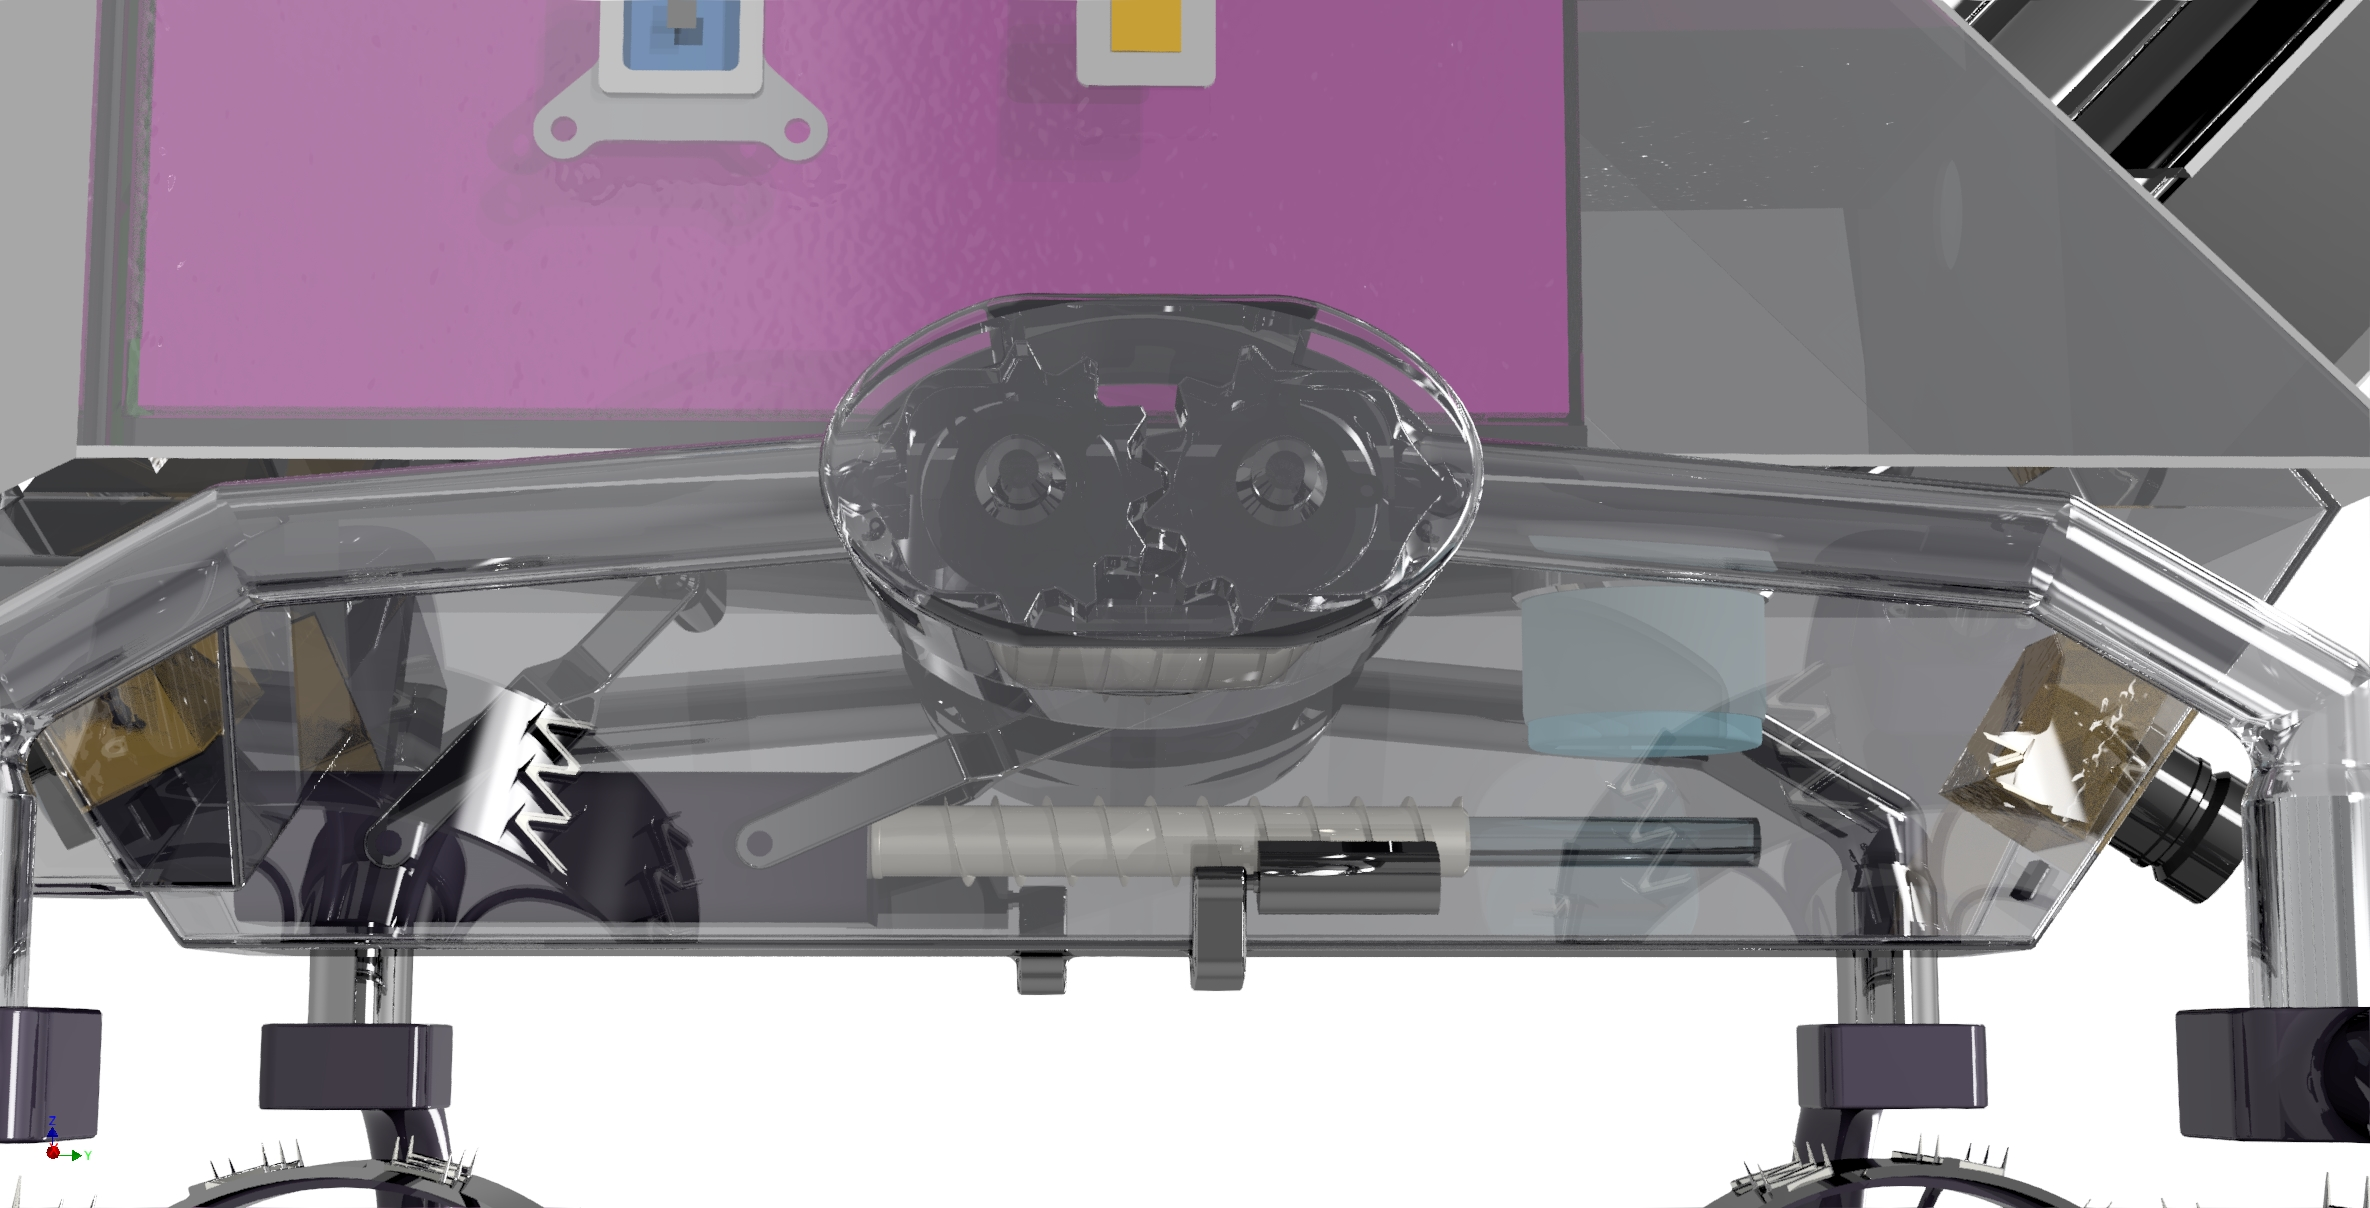
\includegraphics[width=\textwidth]{Media/DrillingBay3}
         \label{fig:stowedDrill}
     \end{subfigure}
     \hfill
     \begin{subfigure}[b]{0.45\textwidth}
         \centering
         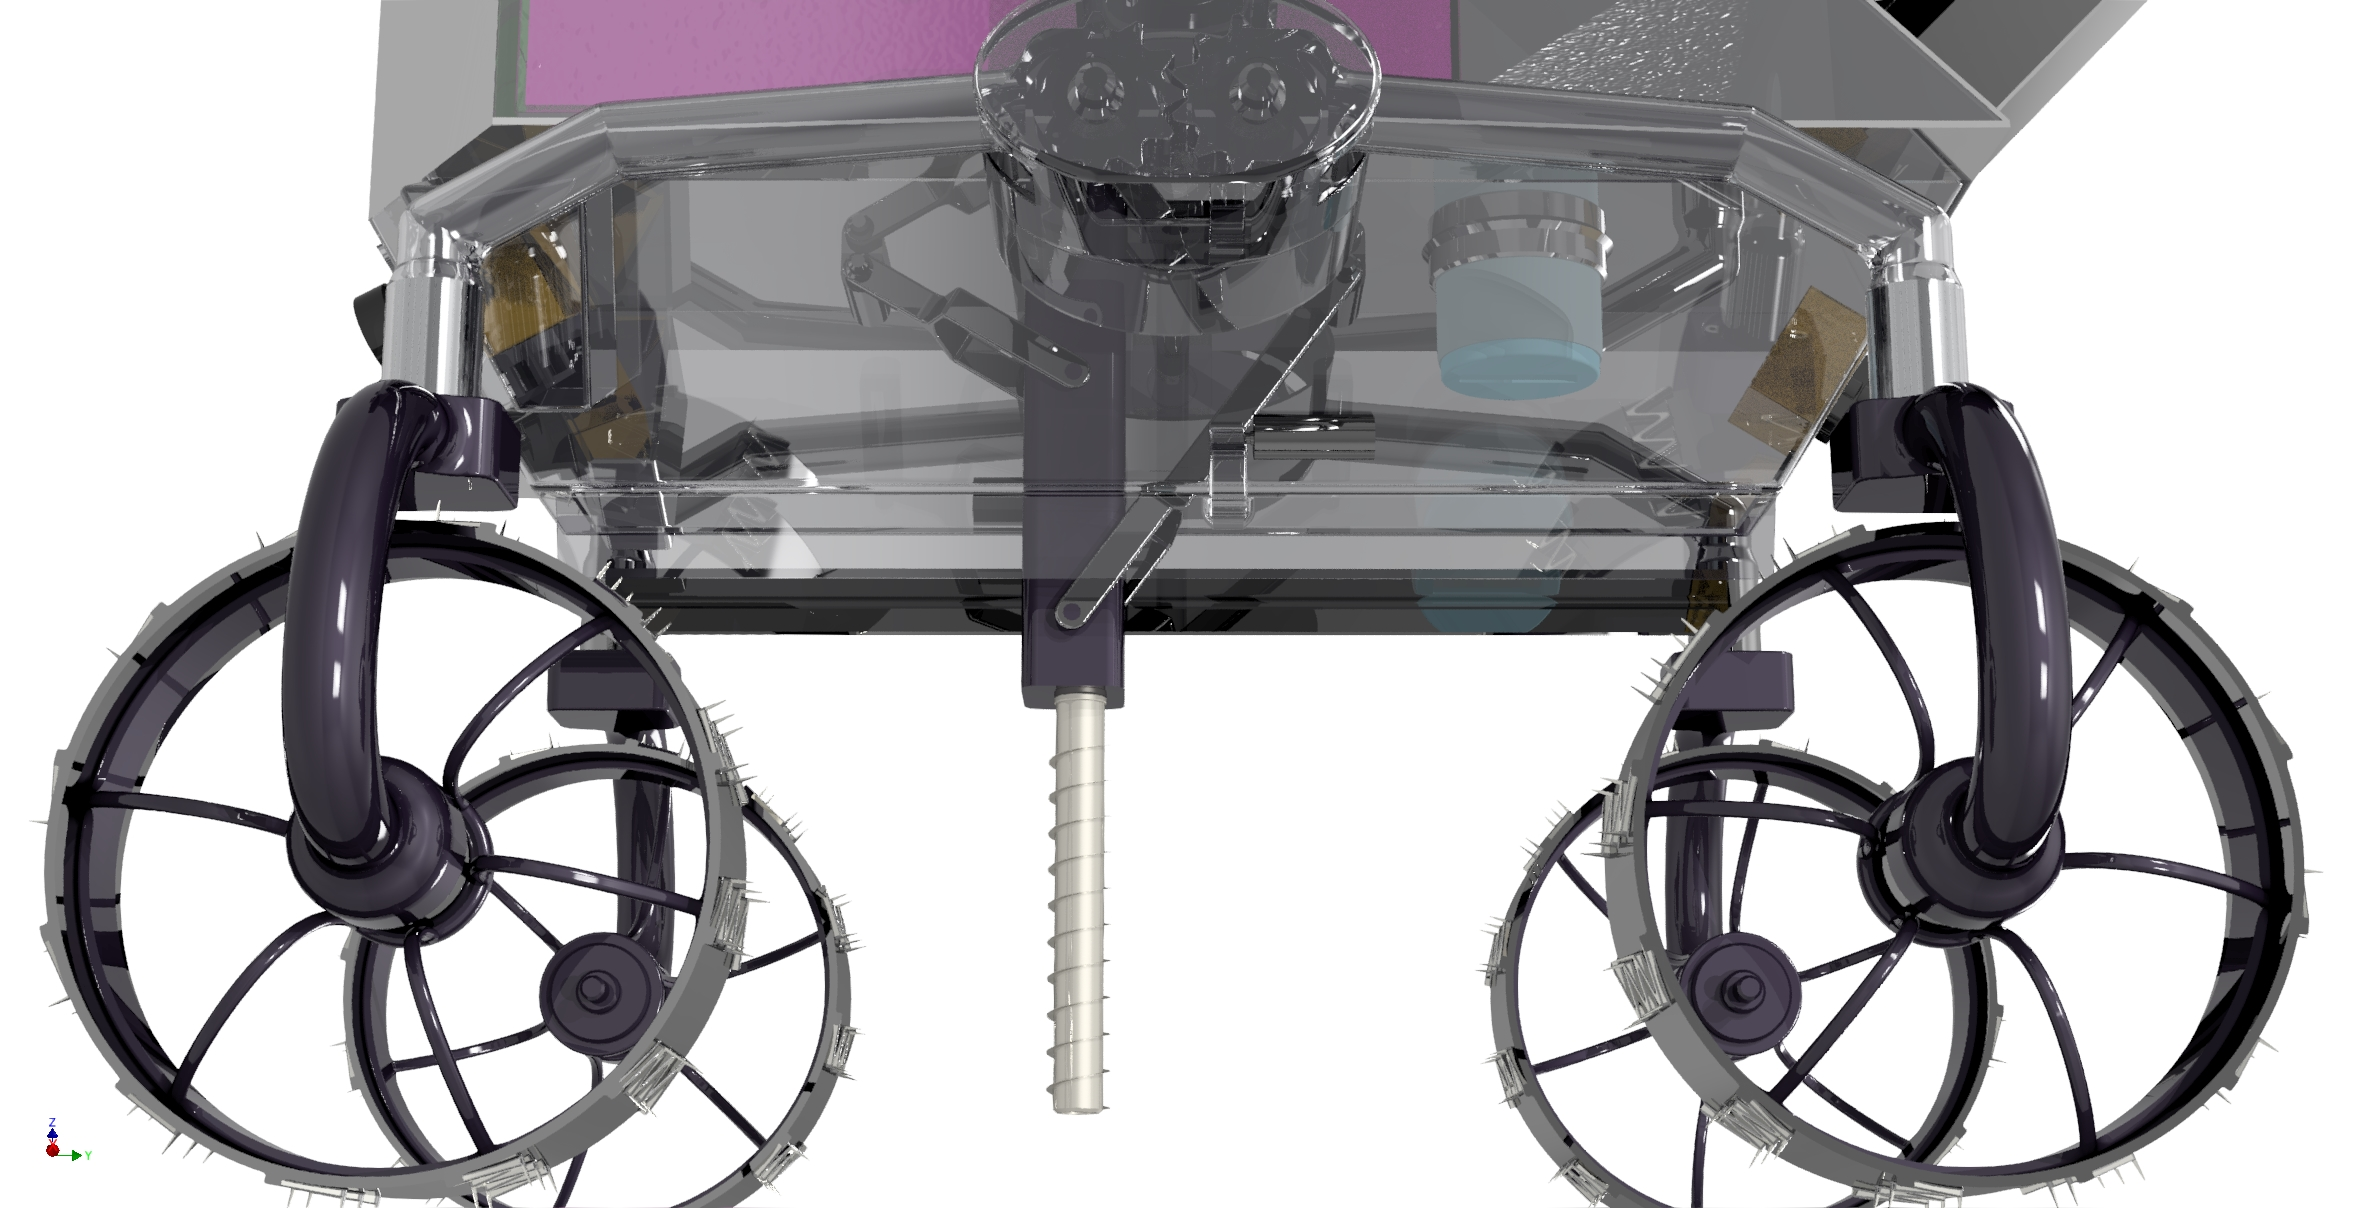
\includegraphics[width=\textwidth]{Media/DrillingBay_unfolded2}
         \label{fig:drillconfig}
     \end{subfigure}
     \hfill
     \caption{Left: Ice Core Drill in stowed configuration, Right: Ice Core Drill in drilling configuration}
     \label{fig:DrillBay}
\end{figure}

\section{APXS Analyser}
The Alpha Particle X-Ray Spectrometer is an analyser that has been used in many explorer missions like the Philae lander or the Mars rover Curiosity, \cite{ref_pay_1} \cite{ref_pay_2}.
The spectrometer uses alpha particles as well as X-rays to identify the sort of atom inside a probe.
The main advantage is the small mass and the  low power it needs during the operation.
As a result of the relatively thin ice core samples, one-third of APXS sources and detectors will used.
Therefore, the mass and power consumption were downsized by one-third because the electronics keep the same and can't be reduced.


\section{Stereovision Camera / Observation / Perception}

The INSPIRE rover is equipped with five individual cameras. Two are used as stereo vision cameras on a hight-adjustable and rotatable telescope arm on the front side of the rover. This is used to capture a detailed 3D model of the environment with which sizes and distances can be estimated. The remaining three cameras are used as hazcams which are necessary to obtain data regarding the nearby environment. All cameras are equipped with radiation-hardened lenses to prevent browning of the lenses. Additional information is provided in \autoref{app:DigitalAppendix}. The main tasks of the camera system are the provision of scientific data and navigation-related data. %More details regarding the navigation and autonomy are provided in \autoref{sec:ControlandAutonomy}. \autoref{fig:CamHEad}

\begin{figure}[htb]
     \centering
     \begin{subfigure}[b]{0.45\textwidth}
         \centering
         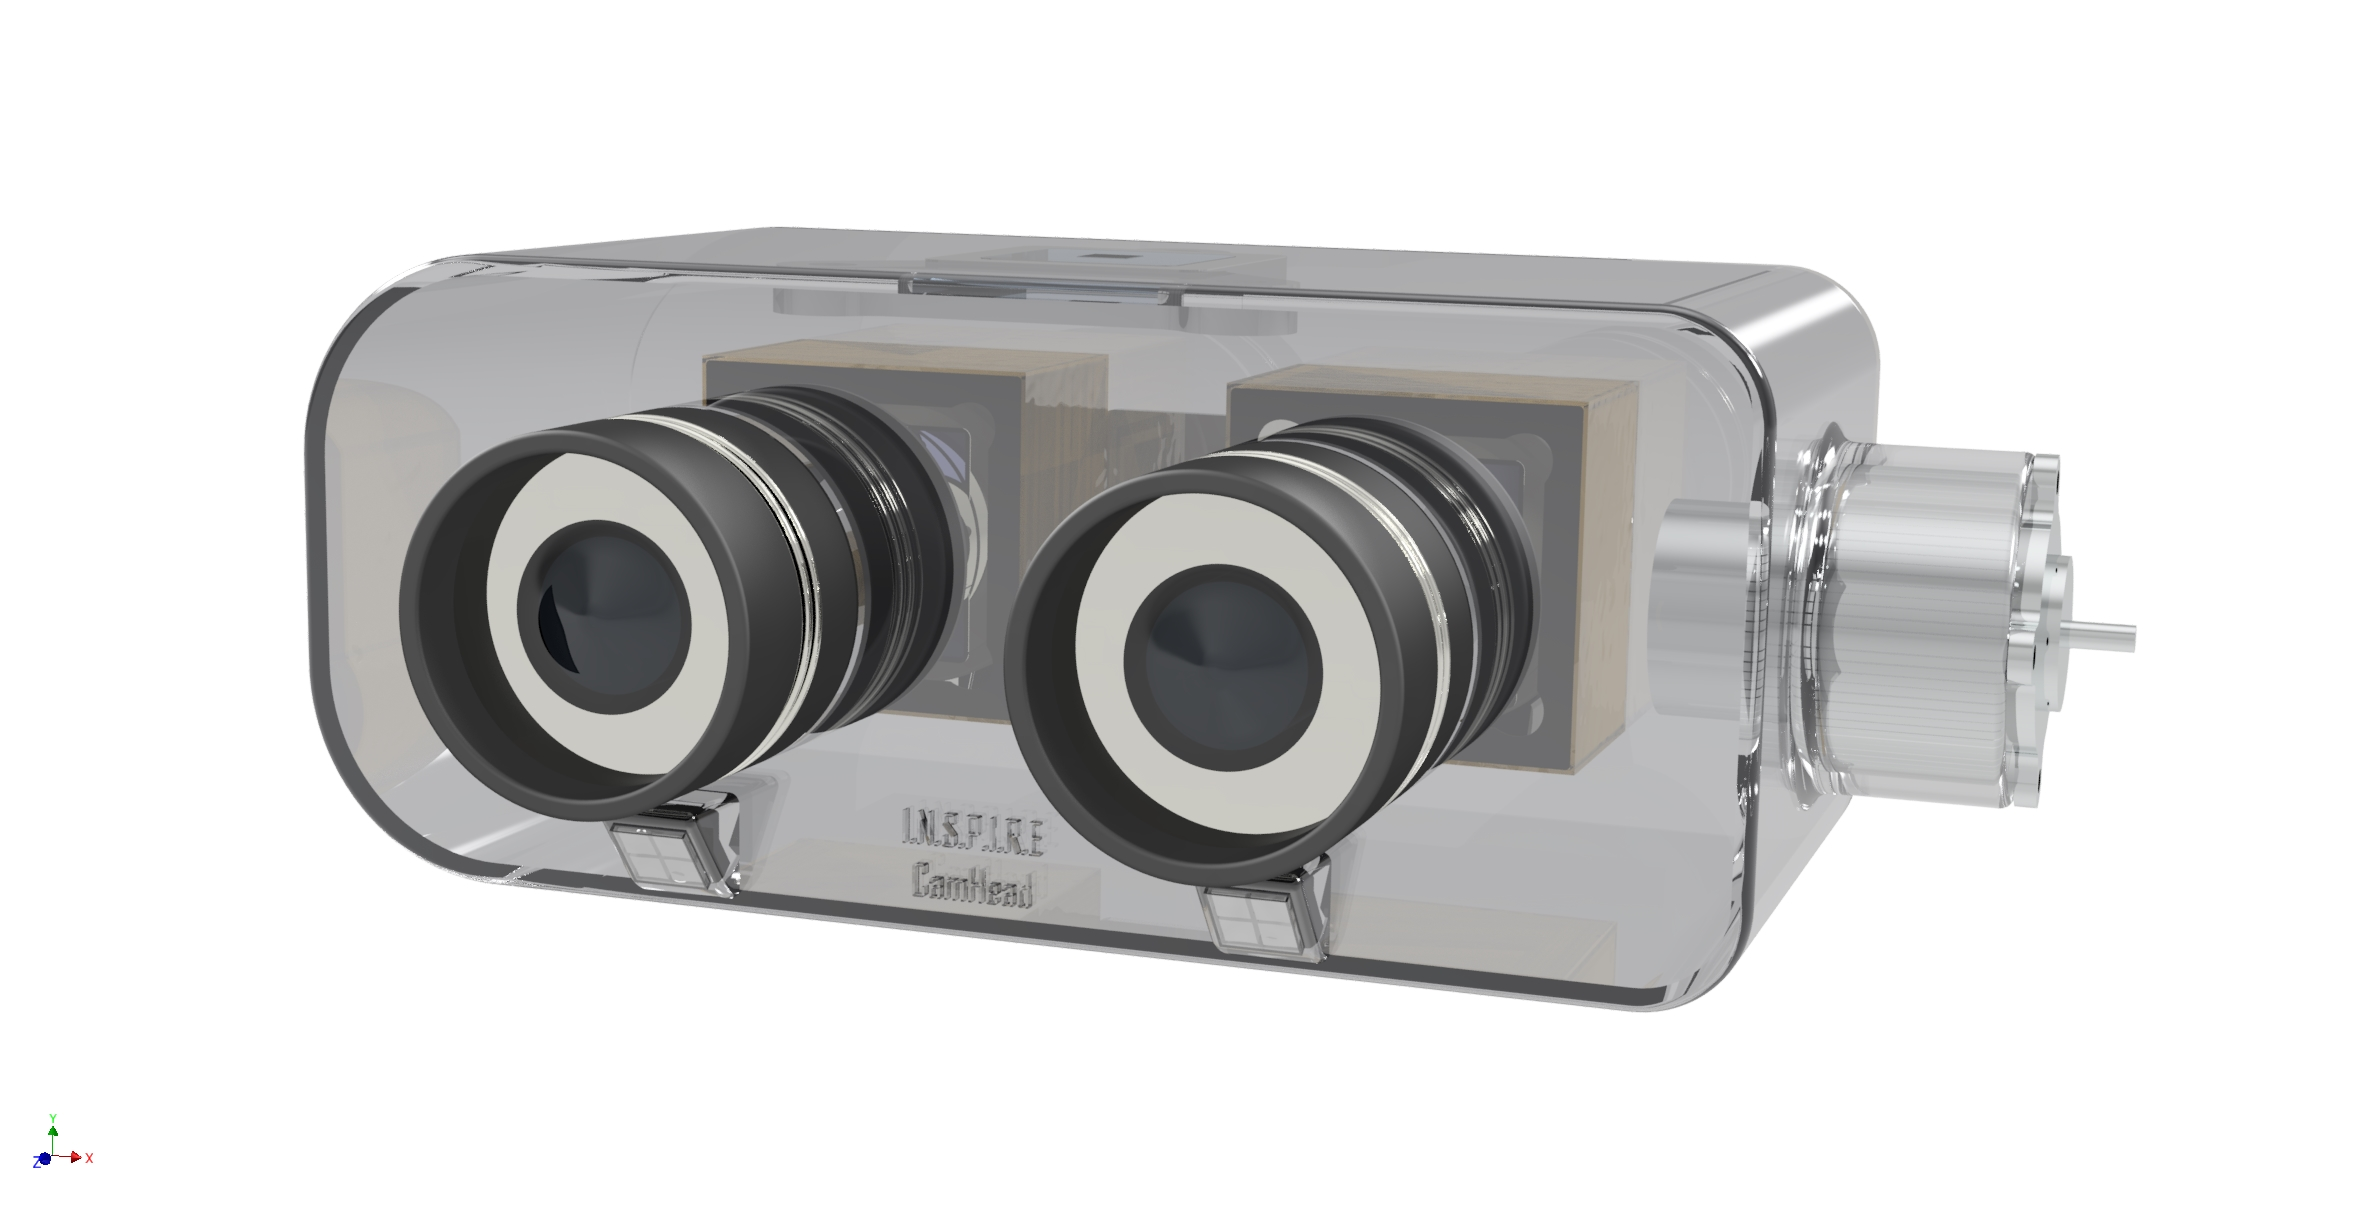
\includegraphics[width=\textwidth]{Media/CamHead}
         \label{fig:CamHead}
     \end{subfigure}
     \hfill
     \begin{subfigure}[b]{0.45\textwidth}
         \centering
         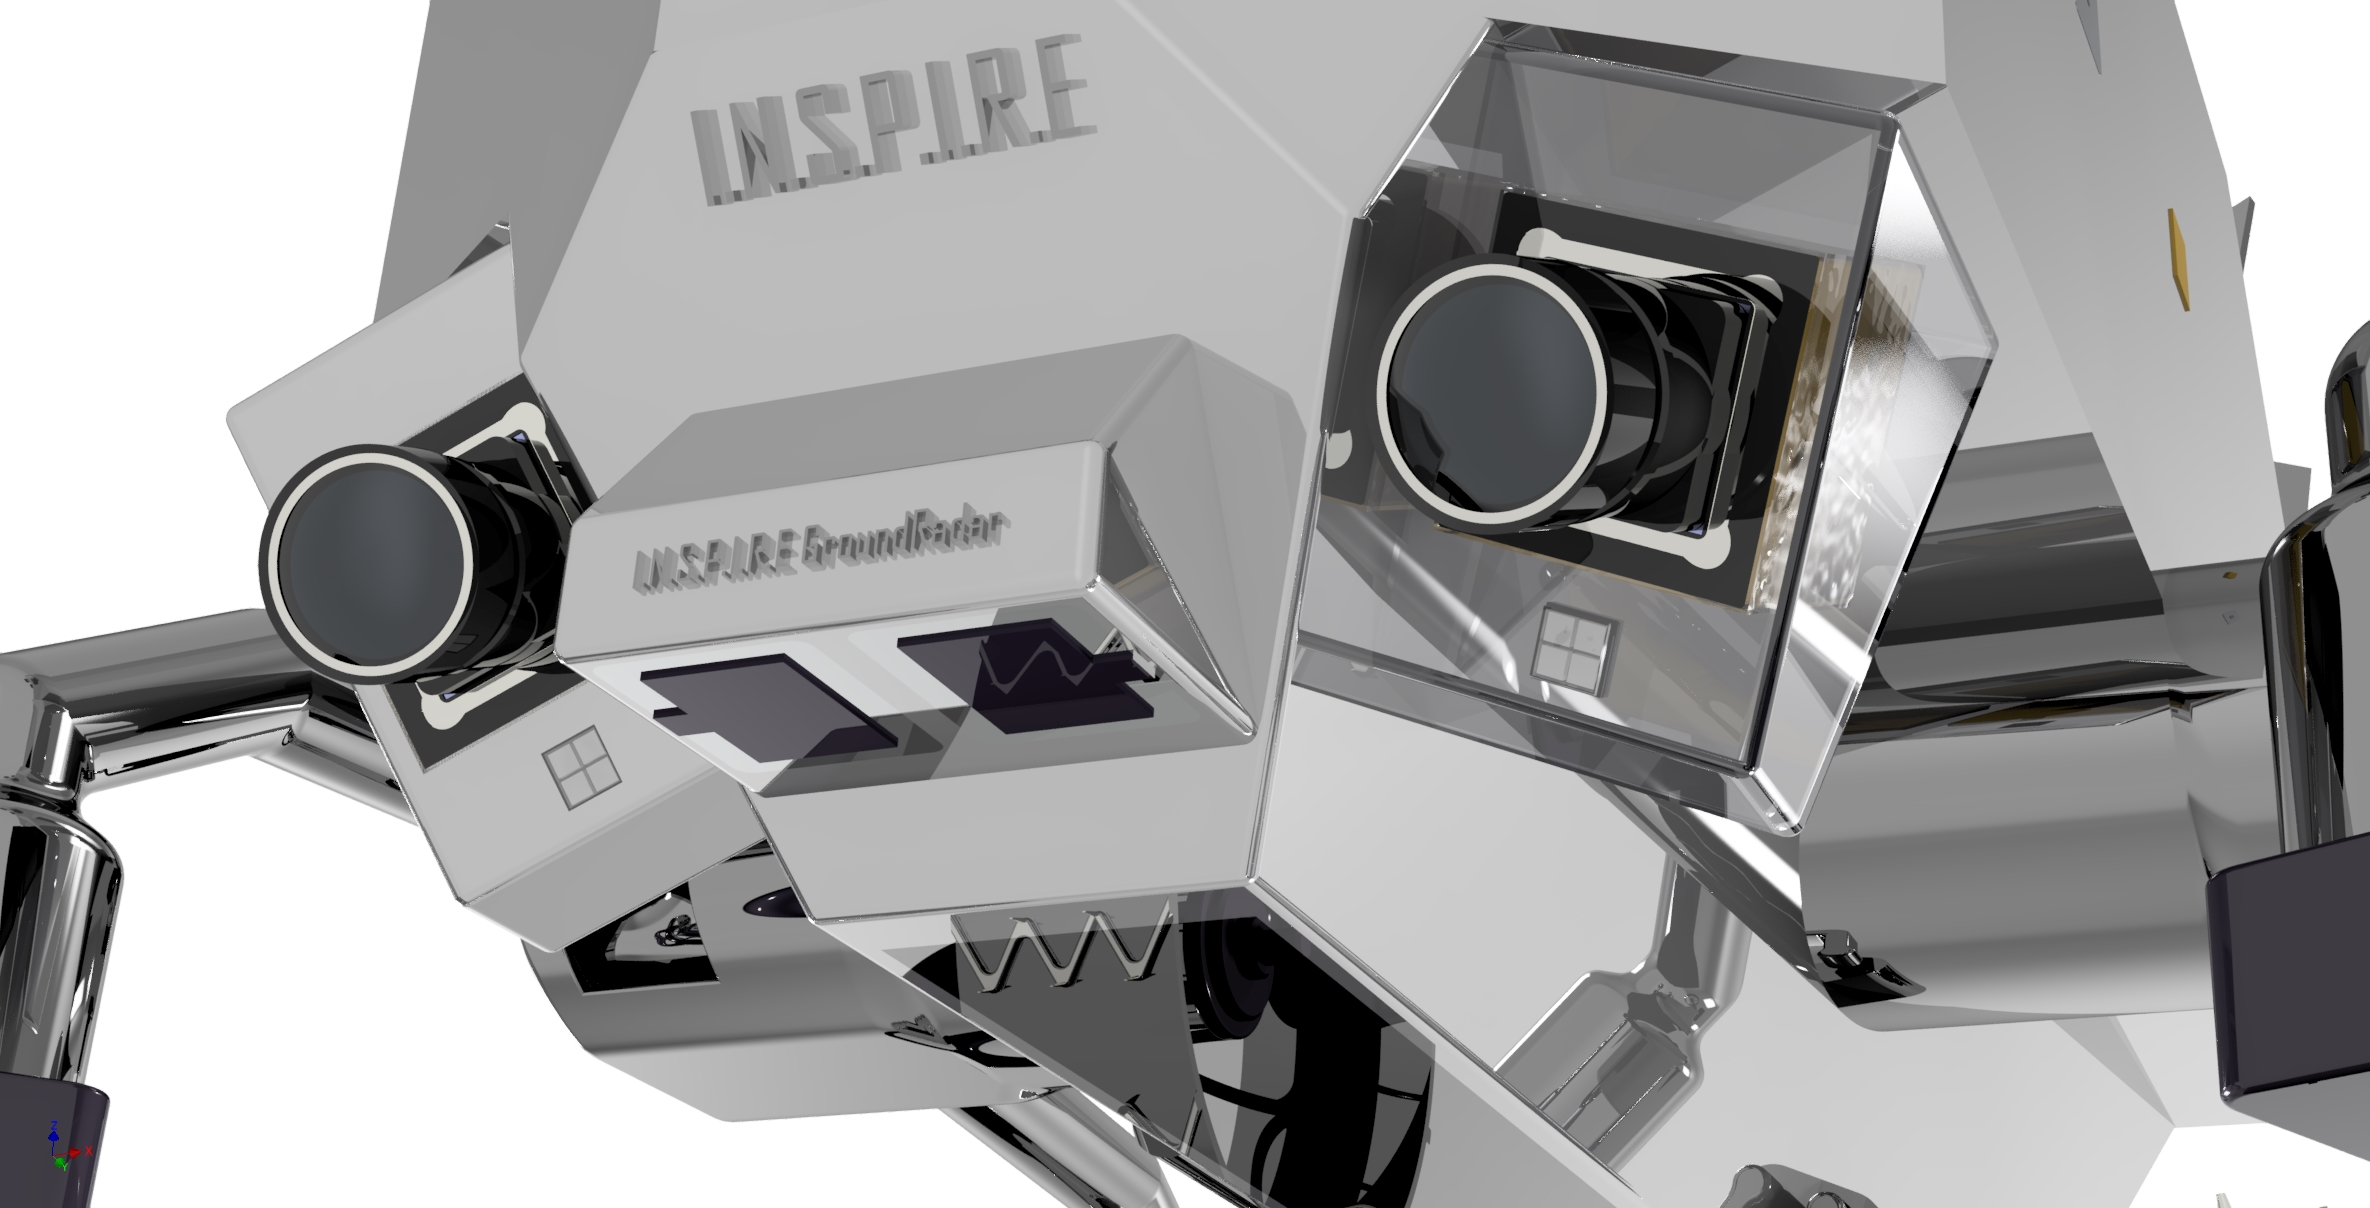
\includegraphics[width=\textwidth]{Media/HazCam_GroundRadar}
         \label{fig:HazCam}
     \end{subfigure}
     \hfill
     \caption{INSPIRE's Surface Observation System including CamHead and Haz Cams + Ground Radar}
     \label{fig:Observation}
\end{figure}

\section{RadHard Solar Arrays}
\label{subsec:radhard}
As a secondary mission goal for INSPIRE, a cooperation with the European project RadHard, led by the German solar array manufacturer Azure Space is intended. The company currently develops a new generation of $4$ Junction solar cells with up to $35~\% $ efficiency. However, the main feature of the new solar arrays is their radiation hardness which will be the high radiation hardness of $>3~\% $ after $1E15~\text{cm}^{-2} \ 1~\text{MeV}$ electron irradiation. Clearly the Jupiter environment, with its extreme radiation environment, represents a suitable destination for a technology demonstration mission. Therefore INSPIRE will be equipped with $10$ RadHard solar cells with a total surface area of $0.0310~\text{m}^2$ for a technology demonstration \cite{FraunhoferInstituteforSolarEnergySystemsISE.2021}.


\chapter{Operation}
\label{chap:Operation}

For the INSPIRE Mission Phase 0 study five basic mission phases have been defined. Nominal mission will last 30 earth days which is equal to 8.47 European days (MISSING REFERENCE). Furthermore a sixth optional mission phase after the nominal mission lifetime has been established which will be conducted if the rover is still operational after its nominal lifetime.

\begin{itemize}
\itemsep0pt
\item	\textbf{Phase 0:} Launch and Flight Phase
\item	\textbf{Phase 1:} Entry, Descent and Landing Phase
\item	\textbf{Phase 2:} Deployment Phase
\item	\textbf{Phase 3:} Egress, Commissioning and Early Operation Phase
\item	\textbf{Phase 4:} Mission Operation Phase
\item	(\textbf{Phase 5:} Exceeding Mission Operation Phase) 
\end{itemize}

\begin{figure}[H]
{\centering
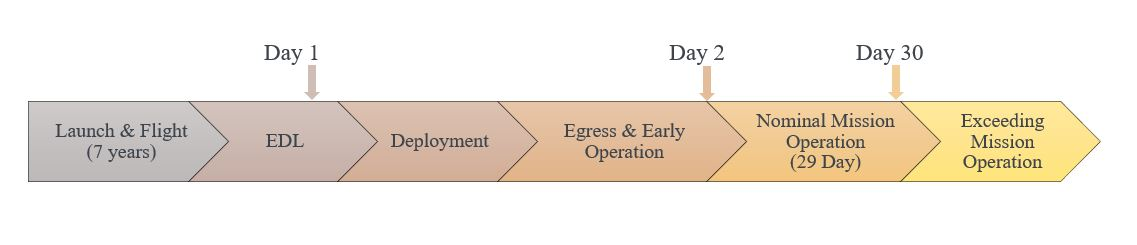
\includegraphics[width=1.0\textwidth]{Media/timeline}
\caption{Preliminary Mission Timeline for INSPIRE.}
\label{fig:timeline}
}
\end{figure}

Based on these missions phases some preliminary rover system modes as well as a basic mission timeline were concluded.

\section{Scientific Output}
\label{chap:sc-output}

Optical reference systems for lath planning limit operation of the rover to an average of 41 h of sunlight (out of 85 h in a European day). \autoref{fig:timeline-day} depicts a breakdown of possible execution times in a mission day based on the power budget. Of course the given order can be changed and execution times can be adapted to fit the mission needs. \\

\begin{figure}[htb]
  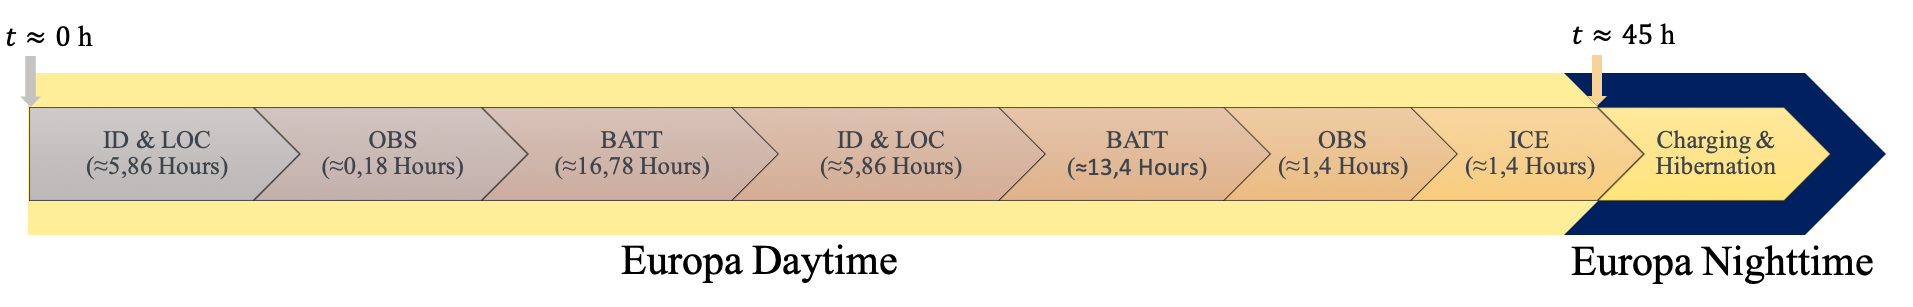
\includegraphics[width=1.0\textwidth]{Media/Timeline_day.png}
  \caption{Timeline of a mission day during phase 4}
  \label{fig:timeline-day}
\end{figure}


Locomotion phases consist of a sequence of mobility packages (MP). Each MP is built up of 5 min path planning and 10 s driving. Path planning time is estimated based on the limited processor speed. \\
Within the 6 h of a single Locomotion phase, a distance of 68 m is covered, resulting in a maximum distance of 1.7 km for the nominal mission.  \\

With respect to the payloads of the INSPIRE mission described in \autoref{chap:payload} the scientific return for phase 4 will consist of the data in \autoref{tab:SciDataOut}. Out of the 9 h of payload operation a total of 6 h is used for imaging and radar measurements. \\
The total data output can be increased further in the case of a sufficient power margin during operation.

\begin{table}[h]
\centering
\caption{Expected scientific data output of the INSPIRE mission }
\begin{tabular}{lll}
Payload         & Data Output                               & Data Output     \\ \hline\hline
GPR             & raw radar measurements                    & 40              \\
Cameras         & grayscale images with optional 3D mapping & >3570 images     \\
Sample Analyser & raw mineral analysis of ice core          & 10 - 12 samples \\
Solar Cells     & performance data                          & continuous      \\ \hline
\end{tabular}
\label{tab:SciDataOut}
\end{table}

  
\section{Rover System Modes}
\label{chap:rovsubmod}
For this case study several rover system modes were defined. All ten modes are listed in \autoref{tab:systemmod}. 

They are separated into two groups. The design critical modes are displayed in white and are defined as system modes, which significantly influence the preliminary design of the rover subsystem like the thermal or power subsystem. None design critical modes (grey) also have a major influence on multiple subsystems of the rover but play a secondary role in the thermal and power budget of the rover for this Phase 0 study. These non design critical modes extend from the rover storage and launch until the finale deployment of the rover is completed. These modes and their design options depend heavily on the final design of the lander with which INSPIRE flies to Europe. Therefore, a clear definition of such modes is not possible at this time in the course of this phase 0 study. However, the respective considerations, preferences and options have been briefly described in the mode descriptions. It is important to note that INSPIRE's goal is to provide a flexible rover design with as few hard requirements as possible for the parent lander. Therefore, many aspects of the rover, as well as the none design critical modes, will need to be further defined and elaborated in later phases of the project in close consultation with the customer. \\
For example, the exact interfaces between rover and lander should be defined in more detail. Depending on the subsequently chosen interfaces, many possibilities may arise in the corresponding rover system modes. With an appropriate interface, for example, the excess electrical and thermal energy of the RTG, which is already active during the flight, could be used to supply the lander system with heat and power. A corresponding interface could also enable the transmission of health checks from INSPIRE. \\
The deployment phase will strongly depend on the final design of the lander, INSPIRE's position within the lander and also the possibilities that the lander provides to INSPIRE.
Possible deployment strategies would be as follows:

\begin{itemize}
\itemsep0pt
\item	\textbf{Option 1:} If INSPIRE on ground level: Release from storage box through spring mechanism or actuators. Rover storage configuration allows rolling and possible motorised actuation
\item	\textbf{Option 2:} If INSPIRE is above ground level: Similar as Option 1 but an additional ramp and ramp deployment would be required.
\item	\textbf{Option 3:} INSPIRE will be deployed through the landers robotic arm if it is capable of lifting its mass.
\end{itemize}

\chapter{Subsystems}
\label{chap:subsystems}

In this chapter, the individual subsystems of the rover system will be discussed in more detail.

\section{Structure and Mechanisms}
\label{sec:mechanics}

The Structure and Mechanisms subsystem mainly deals with the accommodation of the payloads and all components that are necessary for the operation of the rover system. This also includes the mechanisms that are necessary for the rover system to ensure functionality 

\subsection{Storage Configuration and Rover Deployment}

The Main Characteristics of the Rover Chassis design of INSPIRE focuses on compact storage geometry and low Mass. 
During the design process it's been possible to achieve a reduce of volume in comparison to the first INSPIRE chassis design of about xxx~\%.
The geometry data in storage configuration is shown in figure %\autoref{fig:StaticAnalysis}.
The storage volume that is required is 131~l.
For the Rover Deployment there had been a lot of possible concepts, for example a sky crane, a robotic arm or a ramp. Depending of the reason that there are no further informations about the TRIPLE Lander and that the complexity of such a deployment system should be as simple as possible, the decision felt on a ramp where INSPIRE will drive slowly downwards the surface of Europa. 
A possible concept of the rover deployment is shown in the following figure %\autoref{fig:StaticAnalysis}.

\subsection{Exploration Configuration}

When the deployment is successfully done, INSPIRE has to switch from storage - to exploration configuration.
This will be possible with a cogwheel mechanism which will be operated by two Motors (QUELLENVERWEIS). When the wheel forks are horizontal to the ground, the rover is ready for its journey.
In order to maintain the rover stability while driving on rough terrain an averaging differential mechanism is needed.
This will be achieved by a planetary gear with a transmission ration of 1:1.
One bogie then will execute a counter movement du to the tilt of the other bogie.

\subsection{Static Analysis}

As part of the design process, it was necessary to perform a static analysis of the chassis. The following load cases were considered: \\
- Stowed configuration inside the TRIPLE lander on Europa \\
- Exploration configuration on the surface of Europa \\
The analysis was created with the computer aided design software "Autodesk Inventor". 
The results of this analysis are shown in the following \autoref{fig:StaticAnalysis}.

\begin{figure}[htb]
     \centering
     \begin{subfigure}[b]{0.49\textwidth}
         \centering
         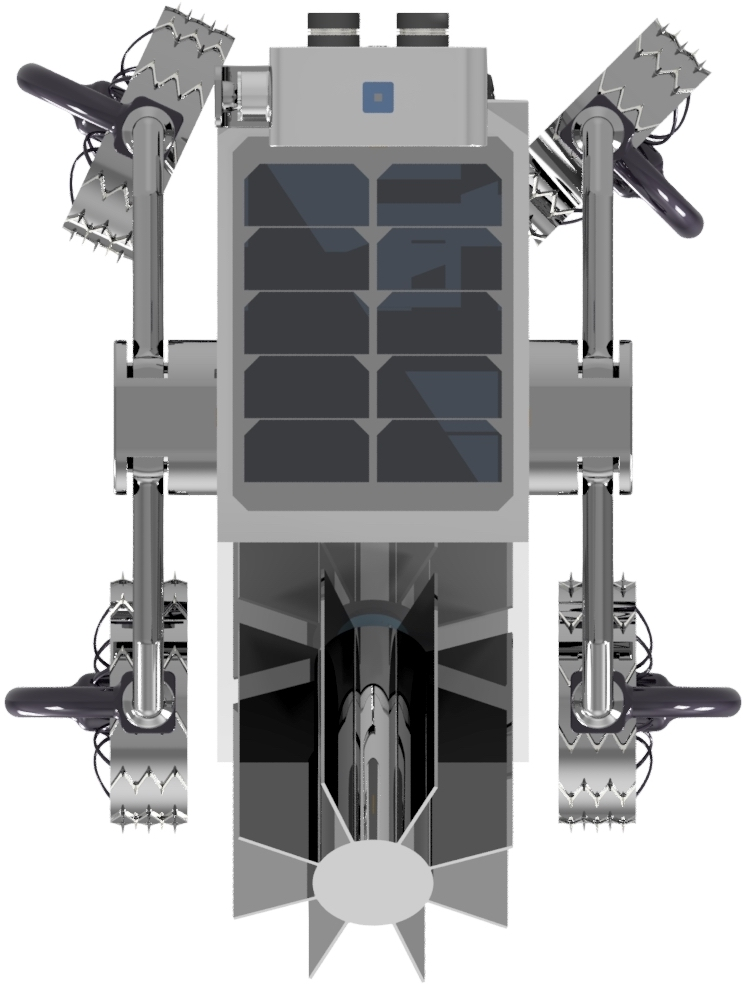
\includegraphics[width=\textwidth]{Media/INSPIRE_Locomotion}
         \label{fig:StoreConfig}
     \end{subfigure}
     \hfill
     \begin{subfigure}[b]{0.49\textwidth}
         \centering
         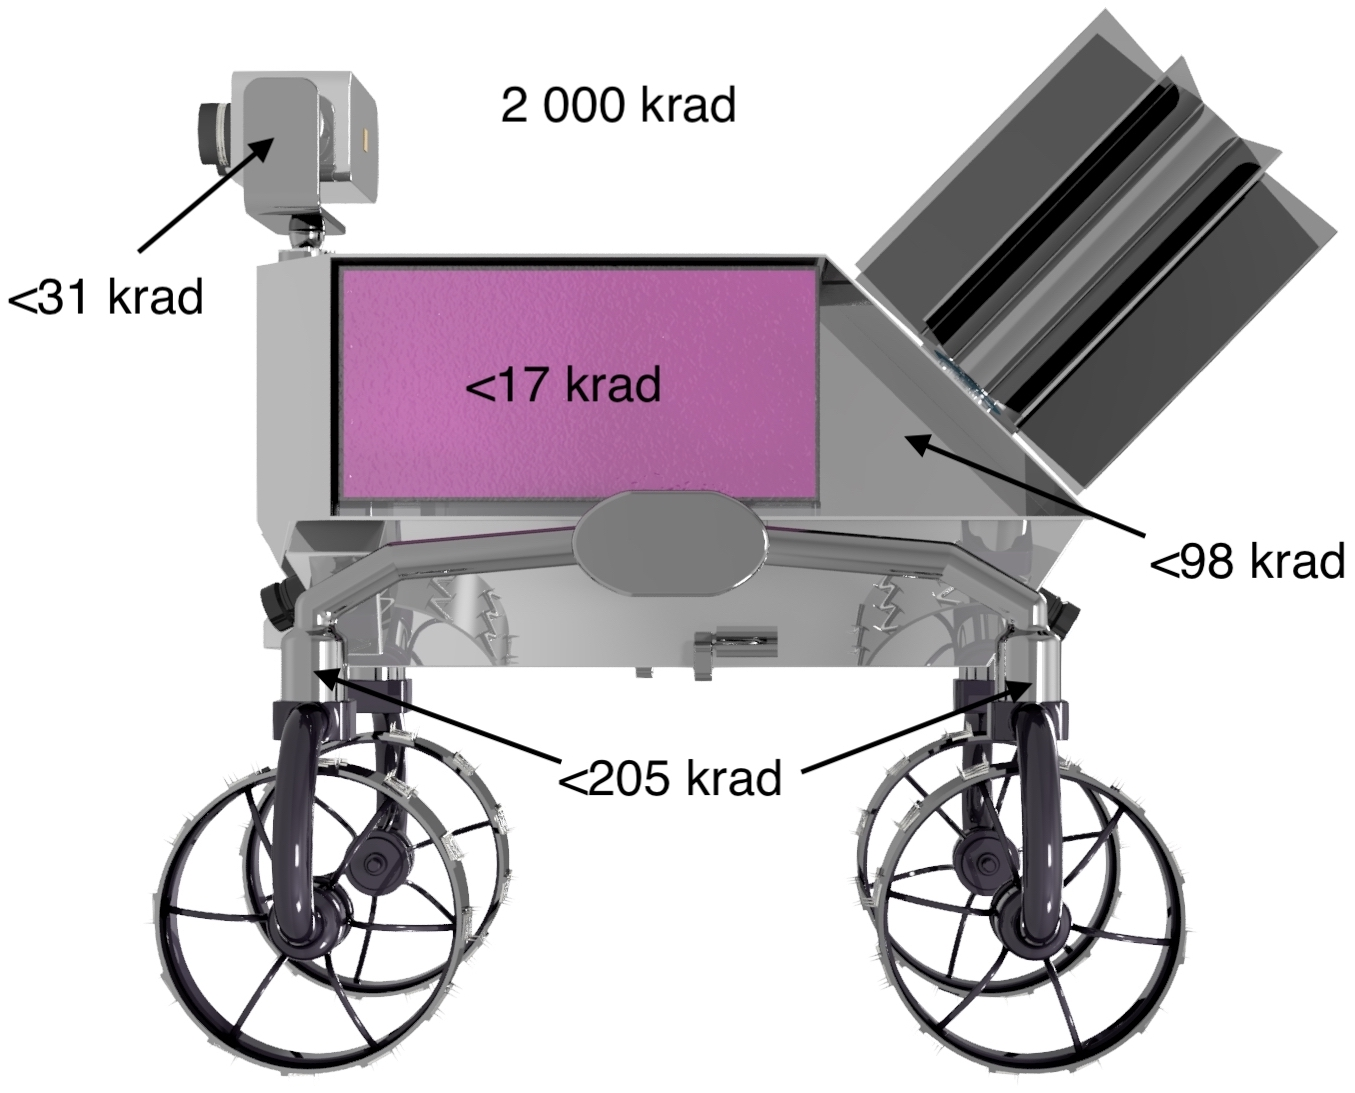
\includegraphics[width=\textwidth]{Media/INSPIRE_Radiation}
         \label{fig:ExplConfig}
     \end{subfigure}
     \hfill
     \caption{Results of the Static Analysis in Inventor. From left to right: Storage Configuration, Exploration Configuration }
     \label{fig:StaticAnalysis}
\end{figure}

\subsection{Mass Budget}

A really important part of each space system is the mass budget. Due to the strict mass restriction, it was quite difficult to find a suitable concept that is both light and space-saving. In order to make the design process of INSPIRE more effective, a specially selected preferred maximum mass of the chassis with the mechanisms of 5~kg was chosen which could also be adhered to. The following table lists the masses of the individual components of the structure and mechanisms system. 
A table with all components of the INSPIRE Rover system is shown in %\autoref{Muss noch verlinkt werden!}.

%-------------------------------------------------------------------------------
\section{Locomotion} \label{sec:locomotion}
%-------------------------------------------------------------------------------

The locomotion subsystem deals with the aspect of how the rover moves and the technical design, including the selection of components such as motors or gears. Before the components can be determined, however, it is necessary to consider certain parameters and design drivers. These will be introduced in the following, and the decisions or estimations concerning the rover will be presented.

\subsection{Design Drivers for Rover Classification}
\label{sec:DesignDriversLoco}

%Initial considerations in the design of a rover's locomotion system are the environmental and operational conditions expected for mission operations, as well as design factors. 
The fundamental rover design can be described by the wheel formula 4x4x4, based on a tradeoff, listed in \autoref{app:DigitalAppendix}. A more detailed design and the main criteria related to this are summarised in \autoref{tab:Design Drivers Rover Movement}.

\begin{table}[htb]
\centering
\caption{Fundamental rover design and the respective design drivers.}
% for the rover movement technique regarding the environmental conditions on Europa and operating conditions.
\label{tab:Design Drivers Rover Movement}
\resizebox{\textwidth}{!}{%
\begin{tabular}{|l|l|}
\hline
\rowcolor[HTML]{B3BBD1} 
\multicolumn{1}{|c|}{\cellcolor[HTML]{B3BBD1}Wheeled System}                                                                                                                     & \multicolumn{1}{c|}{\cellcolor[HTML]{B3BBD1}4-Wheels}                                                                                                \\ \hline
\begin{tabular}[c]{@{}l@{}}One of the most common types of platform\\ - high level of experience\\ - high TRL\end{tabular}                                                       & \begin{tabular}[c]{@{}l@{}}Compared to 2-wheels:\\ - stability  can be ensured \(\rightarrow\) important for drilling\\ - MMP decreases\end{tabular} \\ \hline
\begin{tabular}[c]{@{}l@{}}Compared to other systems:\\ - analysis quite straightforward\\ - simplification \(\rightarrow\) one of the most critical design drivers\end{tabular} & \begin{tabular}[c]{@{}l@{}}Compared to 6-wheels:\\ - less complex \(\rightarrow\) simplification\\ - mass can be reduced\end{tabular}                \\ \hline
\rowcolor[HTML]{B3BBD1} 
\multicolumn{1}{|c|}{\cellcolor[HTML]{B3BBD1}All-Wheel Drive}                                                                                                                    & \multicolumn{1}{c|}{\cellcolor[HTML]{B3BBD1}All-Wheel Actuation}                                                                                     \\ \hline
\begin{tabular}[c]{@{}l@{}}- traction can be increased\\ - increase of \(DP\) and the slope angle \(\theta\)\end{tabular}                                                        & - reduces the risk of slippage on ice                                                                                                                \\ \hline
\end{tabular}%
}
\end{table}

Furthermore, the normal force on Europa can be calculated to \( W \:  = \:	m_\text{total} \cdot g_\text{Europa} \:  = \: 39.45 ~ \text{N} \). Since each wheel is individually driven and controllable, the parameters in the following are designed for one wheel; the normal force per wheel is correspondingly \(W_\text{w} = 9.8625 ~ \text{N}\).

\subsection{System Parameters}
\label{sec:SystemParametersLoco}

Regarding techniques of rover movement, it is crucial to consider the local conditions in which the rover will be operating. The surface of Europa can be assumed to be mainly covered by ice. However, since there are also geysers that transport water to the surface, surface areas may be covered by snow. Though Europa's surface temperature does not exceed 130 K, rather icy, hard-packed snow can be assumed. For this study, a conservative design of the rover is considered, with soil parameters of snow in Sweden as well as heavy clay as a substitute for a hard ice surface; both are listed in \autoref{tab:SoilParam}. Furthermore, the parameters depend on the width and diameter of the wheels of the rover. Therefore, several sizes dependent on the respective weight were selected and a limit per wheel was set to 200 g, illustrated in \autoref{tab:Geometry}. This constraint results in 6 configurations considered for the Rover system design, listed in \autoref{tab:Configurations}. All necessary geometrical dimensions of the locomotion system are shown in \autoref{fig:Ackerman}.

\begin{table}[htb]
\centering
\caption{Configurations for rover classification respective to the wheel width \(b\text{w}\), wheel diameter \(d_\text{w}\) and weight per wheel \(m_\text{w}\).}
\begin{adjustbox}{max width=\textwidth}
\begin{tabular}{cccc|cccc}

	\toprule
		\multicolumn{1}{l}{Configuration} & \multicolumn{1}{c}{\(b_\text{w}\) /m} & \multicolumn{1}{c}{Diameter \(d_\text{w}\) /m} & \multicolumn{1}{c|}{Weight \(m_\text{w}\) /kg} &  \multicolumn{1}{l}{Configuration} & \multicolumn{1}{c}{\(b_\text{w}\) /m} & \multicolumn{1}{c}{Diameter \(d_\text{w}\) /m} & \multicolumn{1}{c}{Weight \(m_\text{w}\) /kg}  \\

	\midrule
		
		1	&	0.05	&	0.1		&	0.127		& 	4	&	0.05	&	0.125	&	0.154	\\
		2	&	0.06	&	0.1		&	0.153		&	5	&	0.05	&	0.125	&	0.185	\\
		3	&	0.07	&	0.1		&	0.178		& 	6	&	0.05	&	0.15	&	0.185	\\

	\bottomrule
	
\end{tabular}
\end{adjustbox}
\label{tab:Configurations}
\end{table}



\subsubsection*{Trafficability Configuration}
\label{sec:DP}

The ability of traffic depends on the soil parameters as well as on the geometric dimensions of the wheels. The sinking depth \(z\) for each wheel of the rover can be determined to:

\begin{equation}
	z \:  = \:	\left( \frac{3 W_\text{w} \cos \theta}{(3-n)(k_\text{c} + b_\text{w}k_\phi) \sqrt{d_\text{w}}} \right) ^{\frac{2}{2n+1}}	.
	\label{eq:Sinkage}
\end{equation}

As shown in \autoref{fig:Sinkage}, the sinking depth \(z\) depends not only on the geometric conditions and soil parameters but also on the slope angle \(\theta\). Therefore, \(z\) can be determined for both soils with respect to \(\theta\) as plotted in \autoref{fig:Sinkage}. However, it can be assumed that for the expected soil, the following applies: \( z_{\text{HeavyClay}} \leq z_{\text{Europa}} \leq z_{\text{Snow}} \).

\begin{figure}[htb]
     \centering
     \begin{subfigure}[b]{0.49\textwidth}
         \centering
         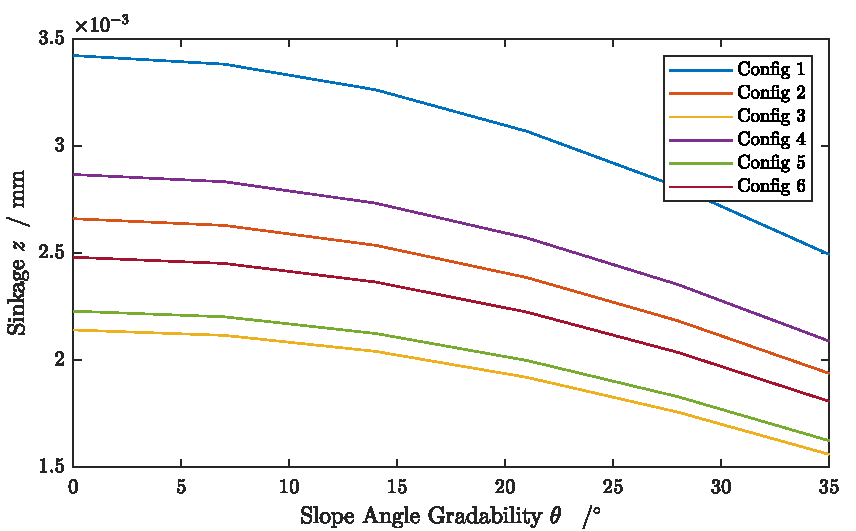
\includegraphics[width=\textwidth]{Media/Sinkage for each config in heavy clay.pdf}
         \caption{Heavy Clay}
     \end{subfigure}
     \hfill
     \begin{subfigure}[b]{0.49\textwidth}
         \centering
         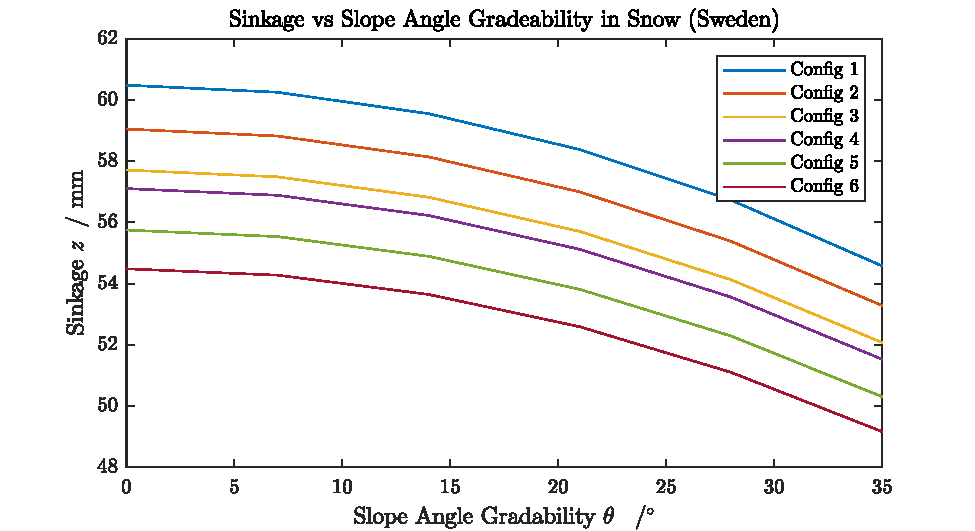
\includegraphics[width=\textwidth]{Media/Sinkage for each config in snow (Sweden).pdf}
         \caption{Snow (Sweden)}
     \end{subfigure}
     \caption{Wheel sinkage \(z\) as a function of the slope angle \(\theta\) of each configuration with different soil parameters, referred to \autoref{tab:SoilParam}.}
     \label{fig:Sinkage}
\end{figure}

The required power for the rover can be calculated by the resistances that have to be exceeded. For the total resistance, the following a applies:

\begin{equation}
 	R_{\text{total}} \:  = \: 
 	\underbrace{R_\text{compaction}}_{= \: \frac{z^{n+1}}{n+1} \left( k_\text{c} + b  k_\phi \right)} + 
 	\underbrace{R_\text{rolling}}_{R_\text{r} = \: W_\text{w}  C_\text{rr}} +  
 	\underbrace{R_\text{gravity}}_{R_\text{g} = \: W_\text{w}  \sin \theta} +
 	\underbrace{R_\text{bulldozing}}_{R_\text{b} \rightarrow 0}. 	
 	\label{eq:Resistance}
 \end{equation} 

Due to the hard surface of Europa, it can be assumed that \( R_\text{b} \rightarrow 0\). In contrast to the \( R_\text{g} \), \( R_\text{r}\) can be defined as constant. With a rolling resistance coefficient of \( C_\text{rr} = 0.02\), the resulting resistance is \( R_\text{r}\) = 0.1972~N \cite{rolling coefficient}. Analogous to \(z\), the lower limit of \(R_{\text{total}}\) with soil properties of heavy clay is plotted in \autoref{fig:RClay}, while the upper limit is shown in \autoref{fig:RSnow} for snow.

In addition to the resistance that needs to be exceeded in order to move, an upper limit can also be determined. The ground thrust \(H\) indicates the maximum amount of traction that can be achieved before the wheels slip.  Therefore, following applies:
\begin{equation}
	H \:  = \: A \cdot c + W_\text{w} \cdot \tan \Phi , 
	\label{eq:}
\end{equation}
 with the wheel ground contact area \(A = \frac{\pi}{4} \cdot b_\text{w} \cdot l\) and the ground contact length \(l = \frac{d_\text{w}}{2} \cdot \cos^{-1} \left( 1 - \left( \frac{2z}{d_\text{w}} \right) \right)  \). As a result, the absolute upper limit of traction is presented in \autoref{fig:HClay} for heavy clay and \autoref{fig:HSnow} for snow. 
 

\begin{figure}[htb]
     \centering
     \begin{subfigure}[b]{0.49\textwidth}
         \centering
         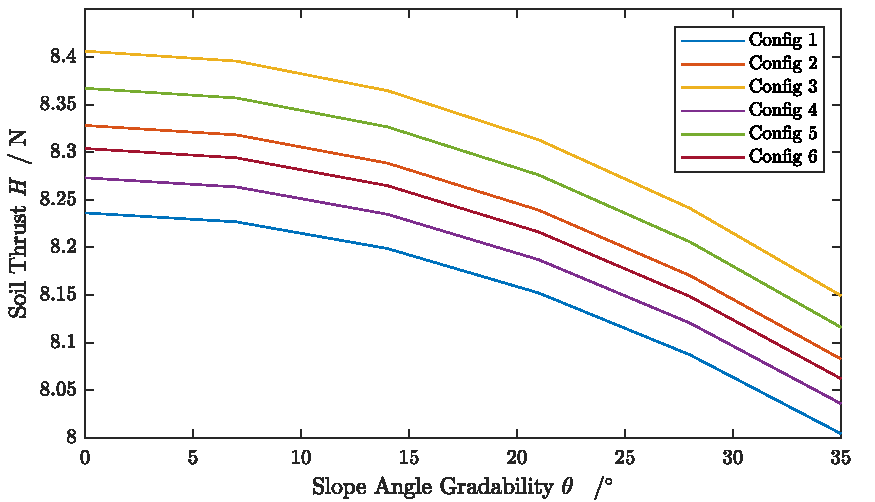
\includegraphics[width=\textwidth]{Media/Soil Thrust Heavy Clay.pdf}
         \caption{\(H\) for Heavy Clay}
         \label{fig:HClay}
     \end{subfigure}
     \hfill
     \begin{subfigure}[b]{0.49\textwidth}
         \centering
         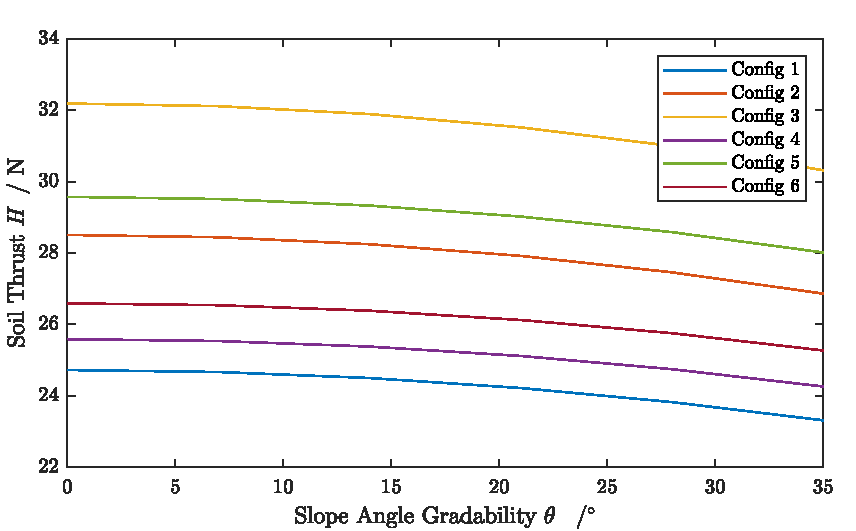
\includegraphics[width=\textwidth]{Media/Soil Thrust Snow.pdf}
         \caption{\(H\) for Snow (Sweden)}
         \label{fig:HSnow}
     \end{subfigure}
     \hfill
     \begin{subfigure}[b]{0.49\textwidth}
         \centering
         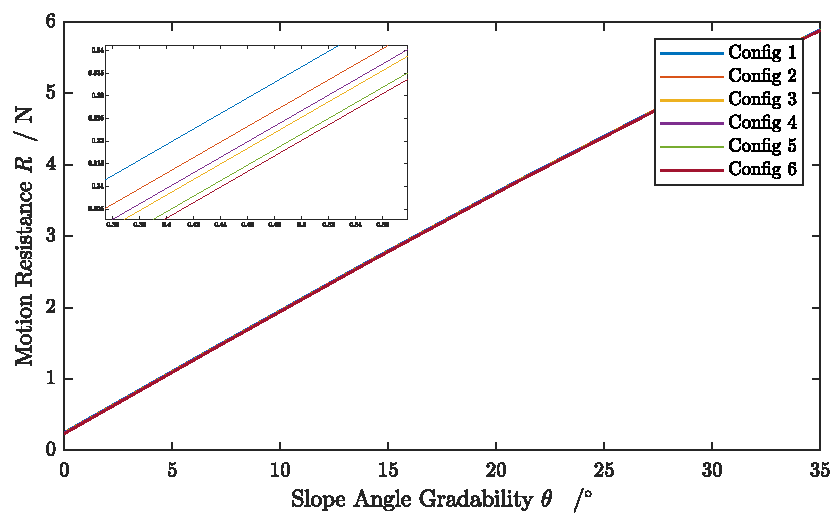
\includegraphics[width=\textwidth]{Media/ResistanceHeavyClay.pdf}
         \caption{\(R_\text{total}\) for Heavy Clay}
         \label{fig:RClay}
     \end{subfigure}
     \hfill
     \begin{subfigure}[b]{0.49\textwidth}
         \centering
         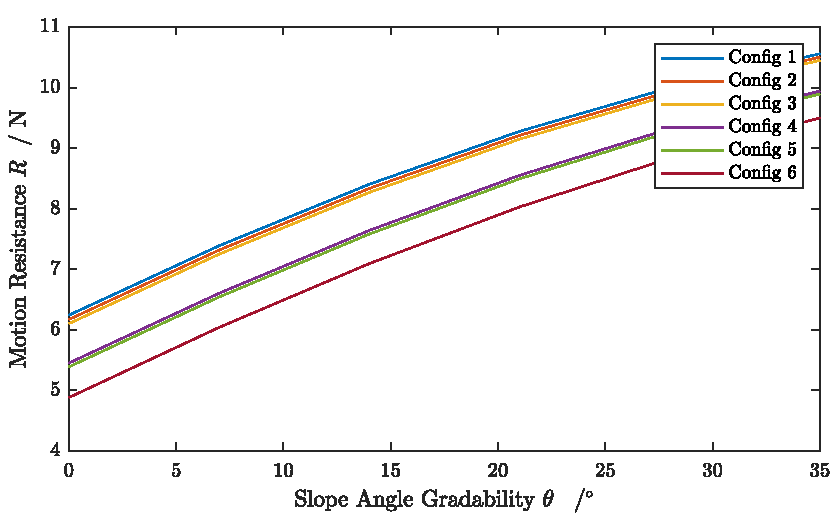
\includegraphics[width=\textwidth]{Media/ResistanceSnow.pdf}
         \caption{\(R_\text{total}\) for Snow (Sweden)}
         \label{fig:RSnow}
     \end{subfigure}
     \caption{Comparison of the rover's soil thrust versus the motion resistance to exceed, each for the soil parameters of snow in Sweden and heavy clay, referenced to \autoref{fig:SoilParameters}.}
     \label{fig:SoilThrust_MotionResistance}
\end{figure}

In addition to the determined parameters, it should also be verified that the mean maximum pressure \(MMP\) does not increase excessively due to the selected geometric parameters. For this conservative calculation, a rigid wheel is assumed, whereby for the deflection \(\delta\) applies, that \( 0 \leq \delta \leq 0.1 d\). For terrestrial snow, 40~kPa should not be exceeded, but ideally the \(MMP\) should be less than 10~kPa. The associated verification calculation can be found in \appref{app:MMP}. \\ 
For the Rover, configuration 6 is chosen as it offers the lowest resistance to exceed whilst maintaining the lowest \(MMP\). It should be noted, that the rover has additional grousers. These are enhancing the traction, whereby the maximum reachable soil thrust \(H\) can be increased. However, the grousers are not taken into account in this study, as this is a conservative estimation, and the grousers can be seen as a further design improvement. 

\subsubsection*{Steering}
\label{sec:Steering}

Since the rover has an all-wheel actuation, it can be operated with on-point steering and, in order to avoid greater obstacles, with Ackerman steering. Considering that with Ackerman steering, the radius of the outer wheels is at a greater distance in the circumventing circle than that of the inner wheels, the angles of the wheel positions, which are important for the control of the rover, can be found in \autoref{tab:Ackerman}.



\subsubsection*{Hardware Selection}
\label{sec:HardwareLoco}

For the wheel driving system, BLDC motors were chosen. In contrast to stepper motors, these are optimised for a uniform torque and not for precise motion control. The resulting power of each wheel can be calculated with respect to the required torque \(\tau\) and the estimated velocity \(v\):

\begin{equation}
	P \:  = \:	\underbrace{\tau}_{= \:	R_\text{total} \left(\frac{d_\text{w}}{2} - \delta \right)} \left(\frac{2v}{d_\text{w}} \right).
	\label{eq:power}
\end{equation}

The motors are designed to produce the minimum achievable power for any soil condition and a slope angle of \(\theta_\text{max.} = 35^\circ\), listed in \autoref{tab:TorquePower} and velocities of \(0.1 \leq v \leq 1\)~m/s are achievable. However, as indicated in \autoref{fig:SoilThrust_MotionResistance}, higher power up to \(H\) can also be generated. Additional planetary gears increase the produced torque with a reduction ratio of 21:1 to \(\tau_\text{max} = 0.5\)~Nm. For the steering system, space grade stepper motors are selected, as a precise motion control is required. Additional information of the motors and gears can be found in \autoref{app:DigitalAppendix}.


\subsection{Deployment mechanism}

The deployment mechanism enables the rover to be stored in the lander in a space-saving arrangement. Two stepper motors are activated in the axle joints for this purpose. In addition, two further inactive motors are installed for redundancy. Stepper motors have the additional advantage that they maximise the holding torque. If in a further design step it should become apparent that the torque is not sufficient, a worm gear could be installed which has a self-retaining function. In addition to deploying after landing, the mechanism is used to reduce the distance to the ground for drilling. 


%-------------------------------------------------------------------------------
\section{Electrical Power System}
%-------------------------------------------------------------------------------
\label{sec:EPS}
The EPS (Electrical Power System) is the subsystem responsible for the electrical power supply of INSPIRE. It consists of four funadmental parts, which are the energy source, the PCDU unit (Power Control and Distribution) and the Energy Storage as well as the rover subsystems as the consumers. The EPS is visualized in \autoref{fig:epsflowchart}.

\begin{figure}[htb]
{\centering
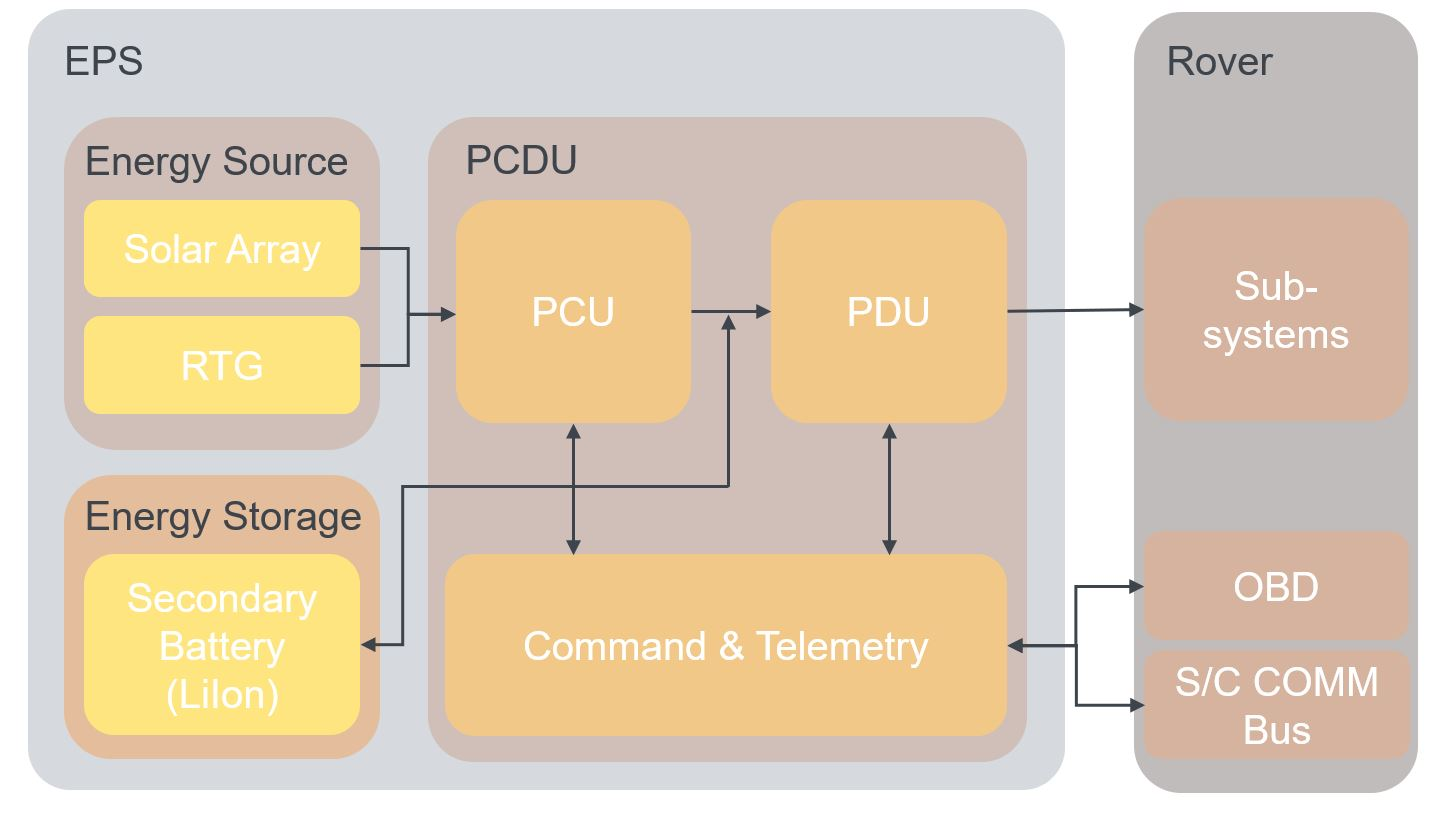
\includegraphics[width=0.7\textwidth]{Media/epsflowchart}
\caption{Functional Flow Chart Diagram for the EPS Subsystem.}
\label{fig:epsflowchart}
}
\end{figure}


\subsection{EPS Budget and Overview}
\autoref{fig:epspowersummary} summarizes the power budget of INSPIRE based on the rover system modes defined in \autoref{chap:rovsubmod}. The holistic power budget can be found in \autoref{tab:powerbudgetcomplete}.
As can be seen, the Locomotion mode has the highest demands on the EPS. The two payload modes also have a high power demand. The Communication mode also has a high consumption. However, since this is primarily used at night and the rover can be charged again afterwards without any problems, it does not place any major restrictions on the power budget. Idle/Perception mode has a low consumption, but is usually used for a long time at a stretch and therefore also places high demands on the EPS. In Charging mode, the EPS is able to charge $8.82 \ W_\text{el} $.


\begin{figure}[htb]
{\centering
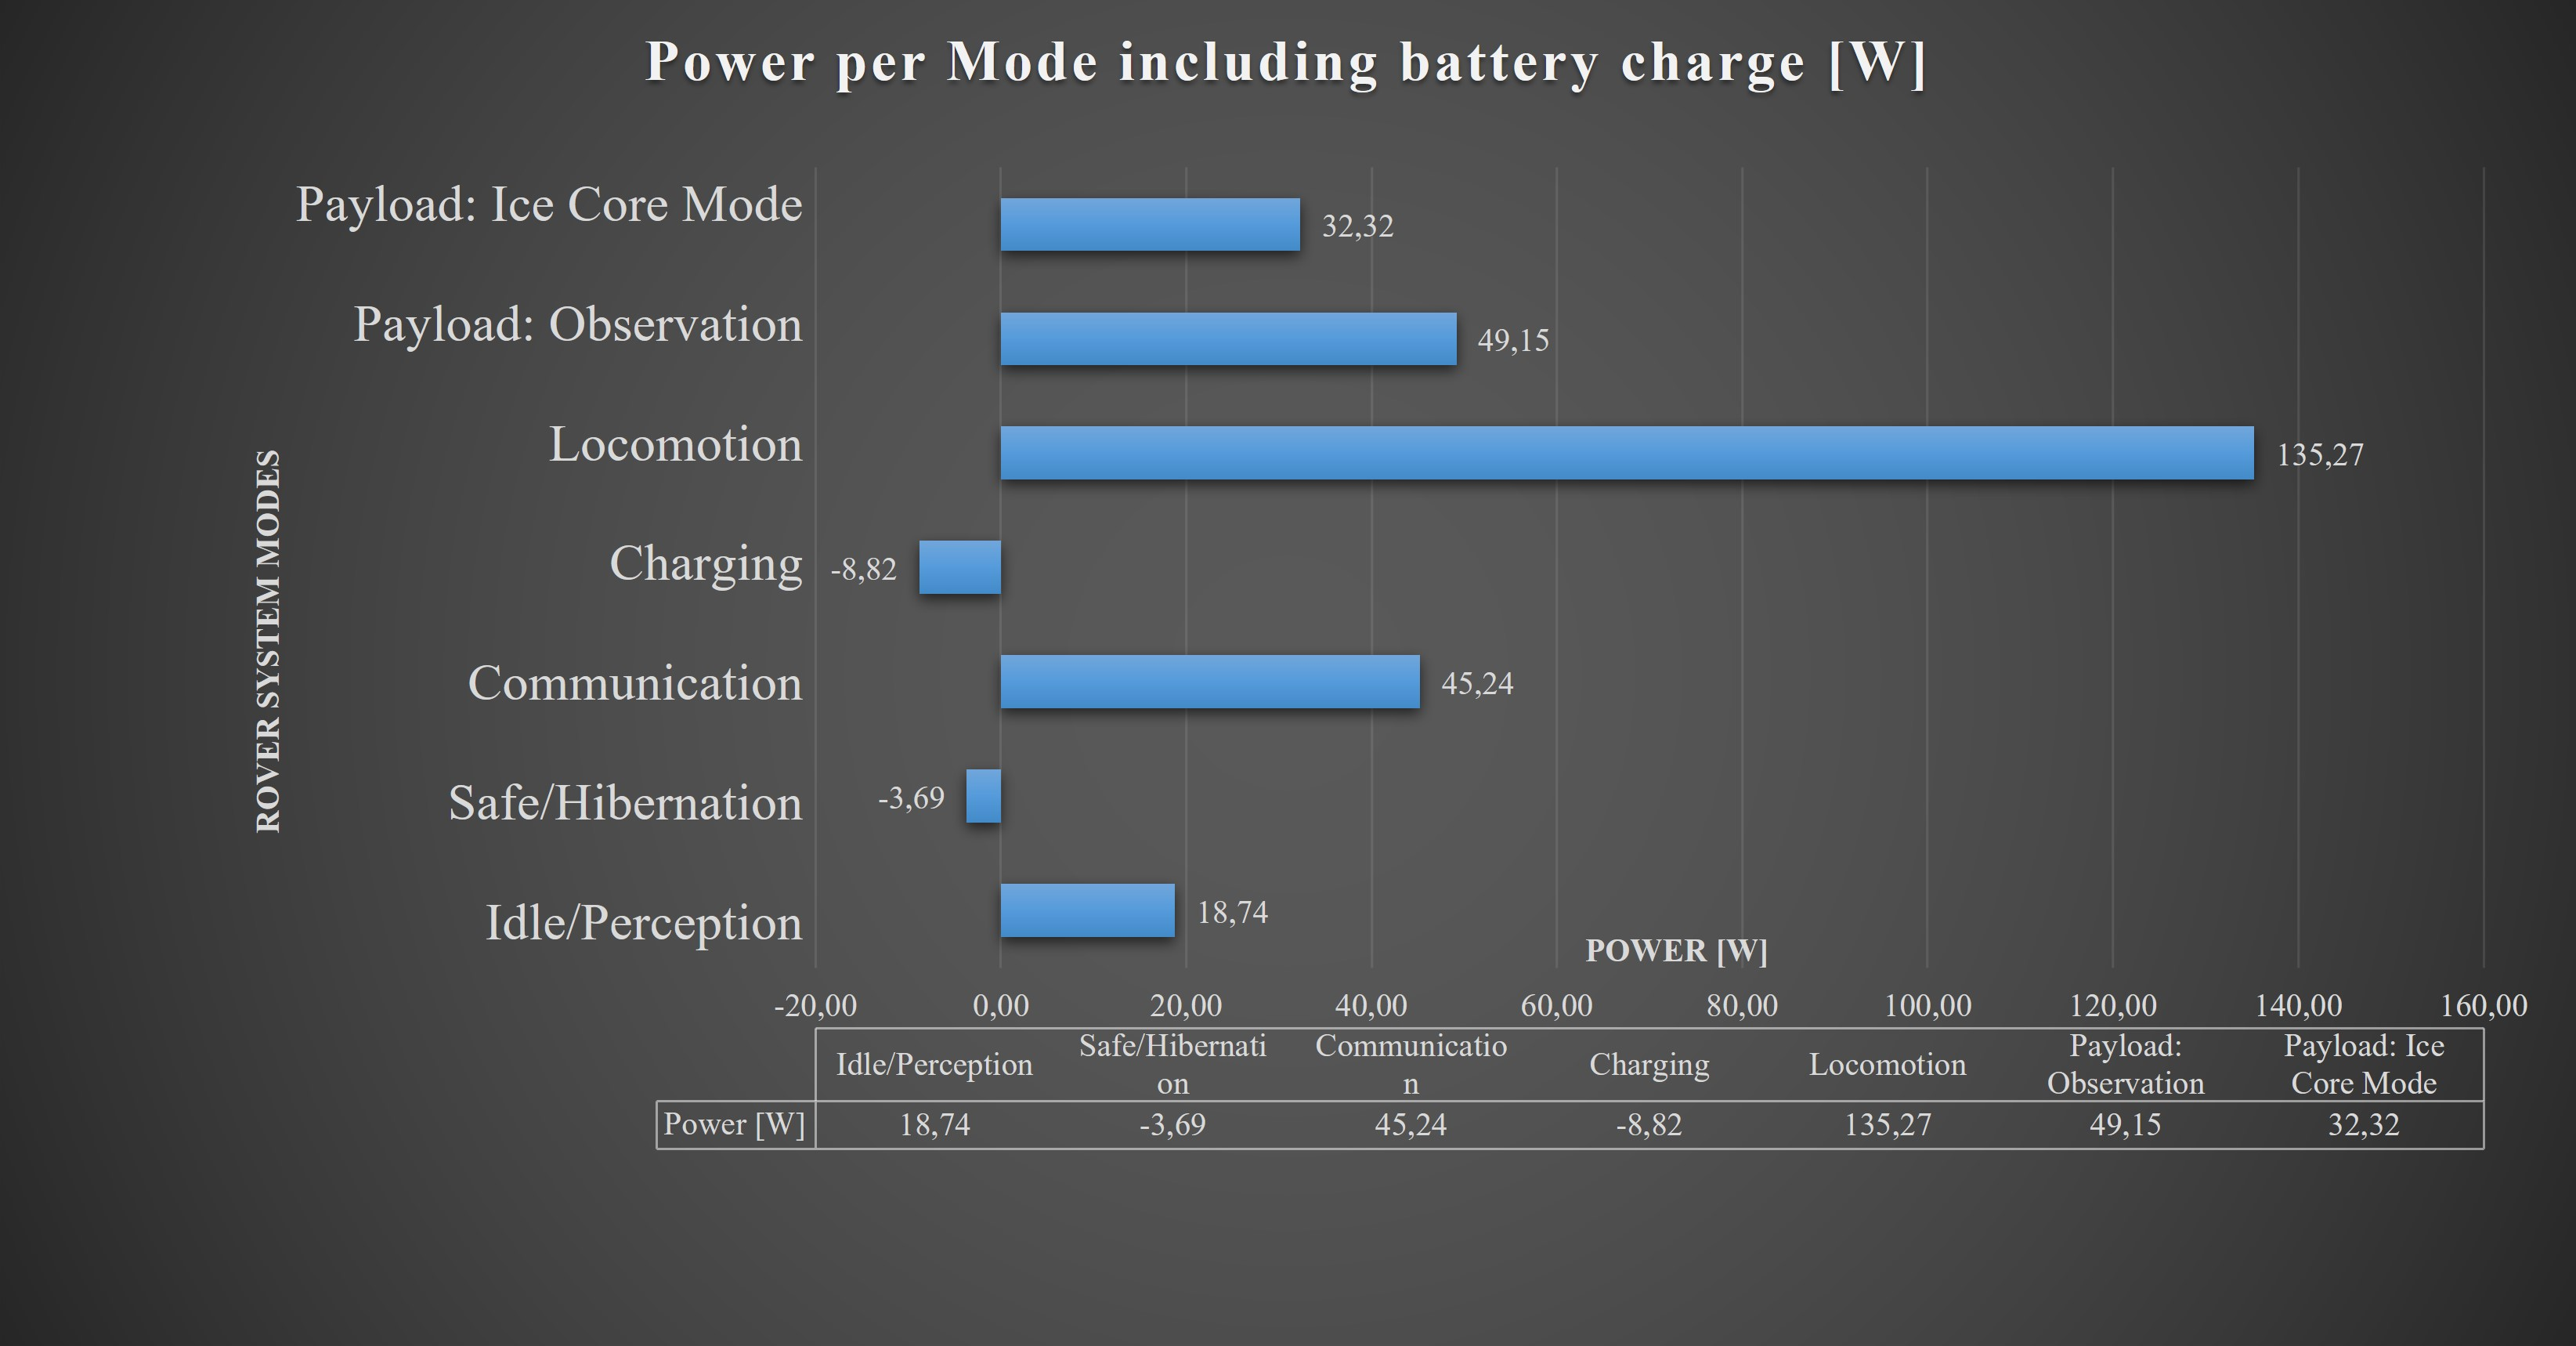
\includegraphics[width=0.7\textwidth]{Media/epspowersummary}
\caption{Functional Flow Chart Diagram for the EPS Subsystem.}
\label{fig:epspowersummary}
}
\end{figure}


%\begin{table}[htb]
%\centering
%\begin{tabular}{|c|c|}
%\hline
%\textbf{Rover System Mode} & \textbf{\begin{tabular}[c]{@{}c@{}}Total Rover \\ Power Demand \\ including battery charge $P_\text{mode}$ [$W_{el}$]\end{tabular}} \\ \hline
%Idle/Perception            & $15.25$                                                                                                                             \\ \hline
%Safe/Hibernation           & $-5.84$                                                                                                                             \\ \hline
%Communication              & $36.92$                                                                                                                             \\ \hline
%Charging                   & $-7.04$                                                                                                                             \\ \hline
%Locomotion                 & $232.36$                                                                                                                            \\ \hline
%Payload: Observation       & $15.41$                                                                                                                             \\ \hline
%Payload: Ice Core Mode     & $9.77$                                                                                                                              \\ \hline
%\end{tabular}
%\caption{Overview of the Power Budget of INSPIRE.}
%\label{tab:powbud}
%\end{table}


\subsection{Energy Source}
For the energy generation of INSPIRE many possible sources were taken into consideration for a trade-off. As a conclusion of this trade-off the decision was made to utilise a Radioisotope Thermoelectric Generator (RTG) as the main energy source for INSPIRE.\\
As the research couldn't find an RTG with a mass suitable for INSPIRE, the solution was to scale down a bigger RTG as an approximation. As a baseline of the scaling the eMMRTG (Enhanced Multi Mission Radioisotope Thermoelectric Generator) was utilised, which is currently under development at NASA and is especially designed for deep space missions like Europa. For the scaling a goal RTG mass of $m_\text{RTG}=3~\text{kg}$ was defined and the eMMRTG was scaled down using the given data.\\
In \autoref{tab:esmmrtg} the scaling results for the eSMMRTG (Enhanced and Scaled Multi Mission Radioisotope Thermoelectric Generator) are listed. The eSMMRTG has a BOL specific power of $\alpha_\text{BOL}= 4.0 \ \frac{\text{W}_\text{el}}{\text{kg}}$ and provides an electrical power of $P_\text{el} = 12.08~\text{W}_\text{el}$ during the mission duration\cite{R.Abelsonetal..2004}\cite{S.Magdum.2019}\cite{Holgate.2015}\cite{eMMRTG.NASA}\cite{Lakdawalla.2018}.



%The outcome of this trade-off is shown in \autoref{fig:epssourcetradeoff} for the most promising energy sources. 

%
%\begin{figure}[htb]
%{\centering
%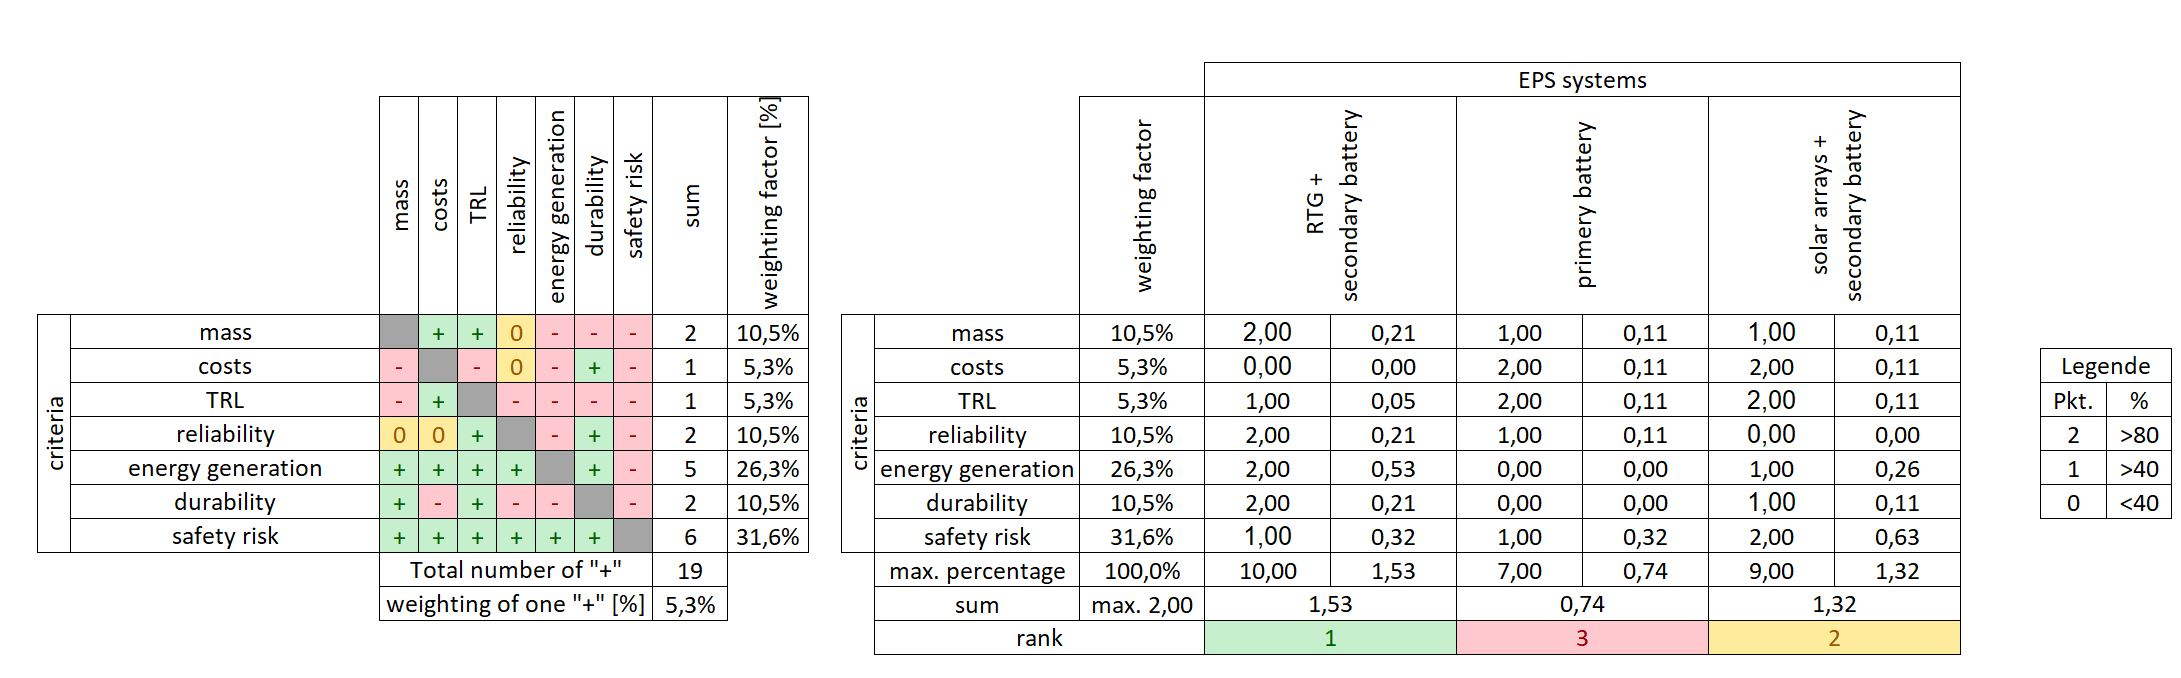
\includegraphics[width=0.7\textwidth]{Media/epssourcetradeoff}
%\caption{Trade-Off Conclusion for the EPS Energy Source.}
%\label{fig:epssourcetradeoff}
%}
%\end{figure}

\begin{table}[H]
\centering
\caption{Parameters for the scaled eSMMRTG based on the eMMRTG.}
\begin{tabular}{lcc}
\toprule
Scaled eSMMRTG Parameter &	Unit	&   Value            \\
\midrule
\textbf{System Mass} $m_\text{RTG}$ & kg  & \textbf{3.5}     \\
BOL Specific Power $\alpha_\text{BOL}$ & $\frac{W_{el}}{\text{kg}}$  & $4.0$     \\
BOL Power $P_{\text{el},\text{BOL}}$ & $ W_{el}$                    & $14$       \\
Isotrop                 &         -                           & Pu-238   \\
Isotrop Half-Life & a                                       & $87.7$     \\
Flight time and Storage (incl. Margins) & a                & $7$        \\
Power Loss Degradation until BOM & $\ W_{el}$                 & $0.56$     \\
BOM Power $P_{\text{el},\text{BOM}}$ & $\ W_{el}$                    & $13.44$    \\
Europa Day Duration & h                                     & $85$       \\
Mission Duration & d                                        & $106.25$   \\
End of Mission Power $P_{\text{el},\text{EOM}}$ & $\ W_{el}$         & $13.42$   \\
\textbf{Final Power for Study} $P_\text{el}$ (incl. $10~\%$ scaling Margin) & $\ W_{el}$  & \textbf{12.08}    \\
\bottomrule
\end{tabular}
\label{tab:esmmrtg}
\end{table}

Furthermore INSPIRE will also be equipped with some radiation hardend solar arrays as already explained in \autoref{subsec:radhard}\cite{FraunhoferInstituteforSolarEnergySystemsISE.2021}. Since these solar cells are primarily used for technology testing, the mission must also be able to operate completely without this generated energy. For this reason, and because the expected energy generated by the solar cells is minimal, only the energy generated by the RTG is considered for the Phase 0 Study. However, it should be noted that these solar cells will also generate a certain amount of energy, which will benefitial for the EPS.


\subsection{Energy Storage} 
For the energy storage of INSPIRE many possible battery types were taken into consideration for a trade-off. As a conclusion of this trad-off the decision was made to utilize LiIon batteries as the secondary batteries of INSPIRE. This decision is primarly based on LiIon batteries high energy density, temperature range, robust performance and long operating and cycle life in extreme environments\cite{IRSatUniversityofStuttgart.2020}\\
As the RTG only generates a small constant power the main energy source during the mission will be the accumulated energy of the batteries. The rover will charge the batteries at night, so the next exploration day can start with full capacity. Furthermore the batteries have to be charged during day time to maintain operations.\\
For the sizing of the batteries, the rover motion was chosen as the design driver, since this is the highest energy consuming state of the rover and additionally mission critical for INSPIRE. The rover motion consists of an interaction of the Locomotion and Perception mode as already mentioned in \autoref{chap:Operation}. Therefore it was defined that INSPIRE shall be able to drive $ 50$ m (including alternating Locomotion and Perception Mode) with a fully charged Battery. Furthermore the battery mass shall not exceed $2$ kg. The required battery capacity $C_\text{Batt,req}$ can be caculated using \autoref{eq:batreq}. The results are listed in \autoref{tab:batsize} \cite{S.Klinkner.2021}.


\begin{equation}
C_\text{Batt,req} = \frac{P_\text{el,req} \cdot t_e }{DoD \cdot \eta_\text{LiIon}}
\label{eq:batreq}
\end{equation}

\begin{table}[htb]
\centering
\caption{Power consumption mode used as design case for the battery sizing.}
\begin{tabular}{lccc}
\toprule
\textbf{Power Consumption Mode:}             &     \textbf{Unit}      & \textbf{Locomotion} & \textbf{Perception} \\
\midrule
Required Electrical Power $P_\text{el,req}$ & $\text{W}_\text{el}$         & $135.27$              & $18.74$               \\
Duration of the mode $t_\text{e}$ & s                         & $500$              & $15000$            \\
$DOD$ for Dimensioning               &     -          & $0.90$                & $0.90$                \\
Efficiency of LiIon Cells $\eta_\text{LiIon}$   &  -  & $0.95$                & $0.95$                \\
Required Battery Capacity per mode $C_\text{mode}$ & Wh & $21.97$              & $91.33$              \\
\textbf{Total Required Battery Capacity} $C_\text{Batt,req}$  & Wh & \multicolumn{2}{c}{\textbf{113.30}}               \\
\bottomrule
\end{tabular}


\label{tab:batsize}
\end{table}

Using these values a suitable battery cell and battery design configuration were conducted. Under consideration of these parameters the battery capacity $C_\text{Batt}$ can be calcuated:

\begin{equation}
C_\text{Batt} = C_\text{cell} \cdot V_\text{cell} \cdot N \cdot M .
\label{eq:batuse}
\end{equation}

According to the ECSS reliability restrictions 1 battery string must be substracted for dimensionsing. Furthermore a $30~\%$ margin on the energy content was applied. This leads to a final battery configuration with a capacity of $C_\text{Batt}=156.24$ Wh and a mass of $m_\text{Batt} = 1980$ g. The final battery values are listed in \autoref{tab:battery} \cite{SAFTBatteries.2018}.


\subsection{EPS Power Control and Distribution}
In order to ensure the full functionality of the EPS, the last main component to be selected is a suitable PCDU. As described in \autoref{fig:epsflowchart}, the PCDU forms the heart of the EPS and is an important interface to the OBC and COMM. Furthermore the PCDU shall be able to monitor and control the rover system if necessary through watchdogs, HPC (High Priority Commands) and direct connections to the OBC and COMM.\\
The PCDU has the challenging task not only to process the RTG as the main energy source, but also to process solar cells as secondary energy sources. Therefore, a PCDU was sought which has the required size, dimensions and range of functions. The research resulted in the Nova PCDU from Bradford DSI. In addition, margins were added to the PCDU to ensure feasibility\cite{BradfordSpace.2019}.

\section{Communications and Command \& Data-Handling}
\label{sec:comm}
The Communications subsystem consists of redundant transmitters and receivers which are cross strapped to four antennas and the OBC. Additionally hard wired connections linking the communication system to the PCDU enable for reboots via direct commands.\\
C\&DH is responsible for the generation of telemetry from the housekeeping boards and the execution of telecommands, as well as the storing and compressing of payload data. 

\subsection{Operational Concept}

Due to power and time constraints, the rover will transmit only telemetry during the locomotion and payload campaigns. Payload data will be compressed, stored and forwarded to the Lander at the end of a mission day. \\ 
 
To achieve the scientific output from \autoref{chap:sc-output} the transmission time per european day is calculated in \autoref{app:MissionDataOutput} (\autoref{tab:Tx-tptal}) and adds up to 38,23 minutes. 
	
\subsection{Communication System}
Requiring too many resources a direct link to earth has been deemed impractical. Instead communication for the INSPIRE mission is proposed to rely on a link between the rover and the Europa Lander. The lander then forwards data to earth via a satellite relay carrier which orbits the moon. The lander offers a 25 dB high gain antenna [Missing Reference] and a low gain antenna which is not further specified in literature.\\

The downlink from the rover to the lander has been identified as the critical transmission path. However, link budget considerations in \autoref{app:LinkBudget} reveal that a transmission to the LGA of the Europa Lander produces a link margin of $10,59~\text{dB}$, resulting in a Bit Error Rate of less than $10^{-4}$. The link budget has been performed under the conservative considerations listed in \autoref{tab:lb-param}.\\

Using the Landers LGA greatly increases robustness due to the elimination of pointing errors and higher margin for rover positioning error. Additionally, the INSPIRE rover’s communication link would not interfere with the Landers communication to the relay carrier by blocking the HGA.

\subsubsection{Component Selection}

Due to the considerably high link margin the focus is on low mass and low power components with flight heritage such as flown on CubeSat missions. Criteria with relatively small impact on the link budget such as component noise or even FEC have not been taken into account. The rover communication uses X-Band for increased compatibility with the lander and has a total system mass of less than $1~\text{kg}$. \\
Since radiation hardness was not included in most data sheets a total dose of $<20~\text{krad}$ was assumed in accordance with values for LEO [Missing Reference]. \\

The selected components are listed in \autoref{tab:ComCompComp}. 

\begin{table}[h]
\centering
\caption{Key criteria of selected communication components}
\begin{tabular}{lll|ll|ll}
Component   & Supplier  & Part Description     & 1. Criteria   & Value    & 2. Criteria & Value          \\ \hline\hline
Transmitter & Sputnix   & SXC-XTX-01           & mass          & 0,195 kg & data rate   & 10 Mbit/s \\
Receiver    & Endurosat & S-Band receiver      & power         & max. 2 W & mass        & 0,220 kg       \\
Antenna     & Endurosat & patch antenna & mass          & 2,2 g    & frequency   & X-Band         \\ \hline
\end{tabular}
\label{tab:ComCompComp}
\end{table}

Expected transmission times per mission day are less than 40 minutes (see \autoref{app:MissionDataOutput}, \autoref{tab:Tx-tptal}). Therefore the transmitter mass is identified as more critical than power. \\
Receiver duty cycles on the other hand range close to 100 \% (REFERENCE POWER BUDGET). Thus power has been identified as the most crucial criteria. \\
A passive X-Band antenna was selected due to compact dimensions and zero power consumption.  \\
The entire trade off can be found in (APP Trade off).

 \subsection{Command \& Data Handling}
 
 With respect to restricted power supply a redundant OBC hot-cold configuration stands to reason. Additionally, the standby mode is suggested during hibernation and charging modes relying solely on the PCDU (see chapter [Missing Reference]). 
Emphasis for the Electronics selection is placed on flight proven radiation hardness to increase mission robustness in the high radiation environment of the Jupiter system. 
Criteria of less importance are CPU speed and dimensions. \\

Instead of designing a new OBC board a trade-off was performed among existing single board computers. SBCs provide peripheral services such as bus interfaces, timer and memory in a flight proven configuration, which promises an effective mission development. \\

BAE Systems provides a SBC with their flight proven Power PC750 Architecture which withstands a total radiation dose of up to $1~\text{Mrad}$. The robustness comes at the cost of a $182~\text{MHz}$ processor speed (DATASHEET REFEreNCE). \\

Additionally a custom housekeeping board will be tasked with providing engine control peripherals and sensor read out electronics. 

%-------------------------------------------------------------------------------
\section{Thermal Control System} \label{sec:thermalcontrol}
%-------------------------------------------------------------------------------
The main object of the Thermal Control System (TCS) is to keep the eletric components within their temperature limits, listed in \autoref{tab:tcs_limits}.
As a result of Europas low surface temperature, a small solar constant and the thin atmosphere the heat loss of the rover has to be minimised  \cite{Europa}.

\subsection{Concepts}
The main heat source of the rover is the waste heat of the RTG (see \autoref{sec:EPS}), which will be lead by thermal straps to the thermperature sensetive components.
Carbon-based straps \textit{LyNX}\textsuperscript{\tiny\textregistered} with a high thermal conductivity to density ratio will be used, \cite{ref_tcs_01}.
However, the thermal conductivity is highly depend on the materials temperature, see \autoref{fig:tcs_strap01}.
The curve was aproximated by an qubic interpolation, \autoref{fig:tcs_lynx} and \autoref{eq:tcs_lynx}.
To consider heat loss as a result of surface contact and radiation, the thermal conductivity was reduced about 20\% ($f_{r}=0.8$).


\begin{figure}[h]
	\centering
	\subfloat[Temperature dependent thermal conductivity/density of \textit{LyNX}\textsuperscript{\tiny\textregistered} (yellow curve), copper, and aluminum, \cite{ref_tcs_01}.]{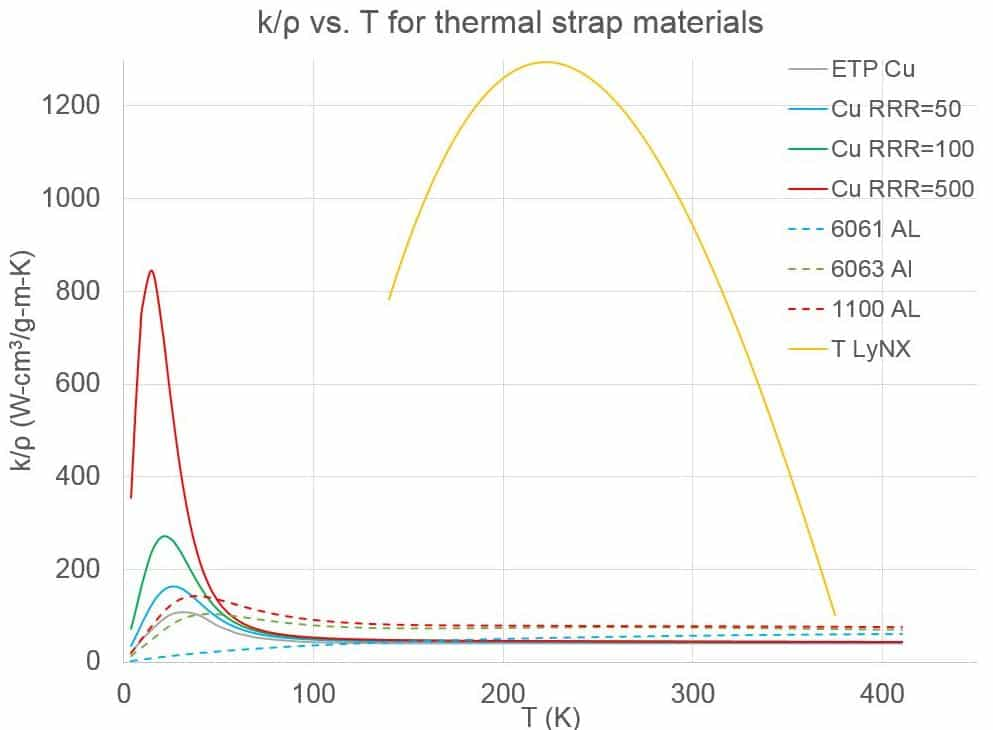
\includegraphics[height=0.3\textwidth]{Media/tcs_strap_01.JPG}\label{fig:tcs_strap11}}\qquad\qquad
	\subfloat[Example of a thermal strap, \cite{ref_tcs_01}.]{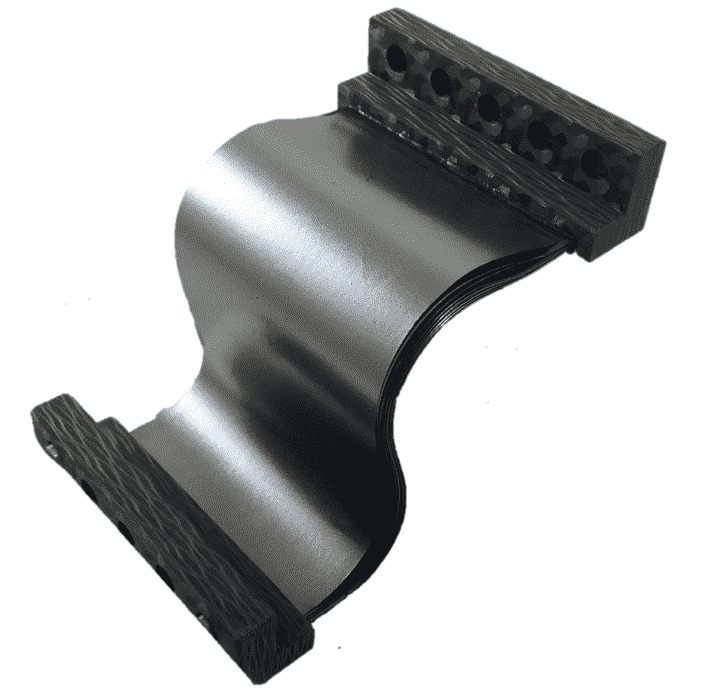
\includegraphics[height=0.2\textwidth]{Media/tcs_strap_02.png}\label{fig:tcs_strap12}}
	\caption{Carbon-based thermal strap \textit{LyNX}\textsuperscript{\tiny\textregistered}.}
	\label{fig:tcs_strap01}
\end{figure}


The camera, exposed on a mast, will be heated by a seperate, light weight Radioisotope Heater Unit (RHU), which has  been used during several NASA missions \cite{ref_tcs_02}.
For the insulation, the material \textit{Aerogel} will be applied, which has a very low heat conductivity, \cite{ref_tcs_03}.

To avoid the risk of overheating, concerning the ebay, camera and drive engine, passive bi-metallic heat switches (see \autoref{fig:tcs_switch01}) will be  placed between the application and the connection interface.
These switches change their heat conductivity beyond a certain temperatur due to the expansion of the disk (see \autoref{fig:tcs_switch21}).
It was assumed, that the toggle temperatur can be adapted by increasing the disk height.
The influence of the changed disk stiffness on the contact pressure and therefore the heat conductivity was neglected for this study.
The measured heat conductivity characterisitc was divided in three linear sections (\autoref{fig:tcs_switch22}), to enable a simple modelling in the thermal calculation.
For the most componets, a cost-efficient sand blasting of the surface is applicable.
For special requirements, white paint will be used, \autoref{tab:tcs_surf}.

\begin{figure}[H]
	\centering
	\subfloat[Closed switch, high heat conduction.]{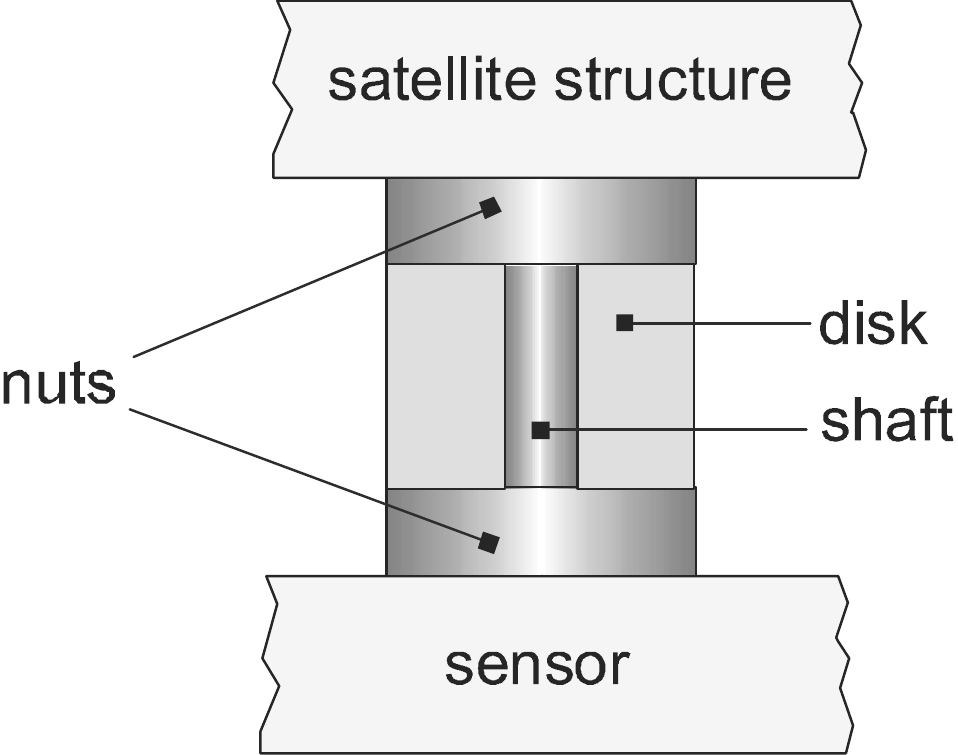
\includegraphics[height=0.18\textwidth]{Media/tcs_switch_01.png}\label{fig:tcs_switch11}}\qquad\qquad
	\subfloat[Open switch, reduced heat conduction.]{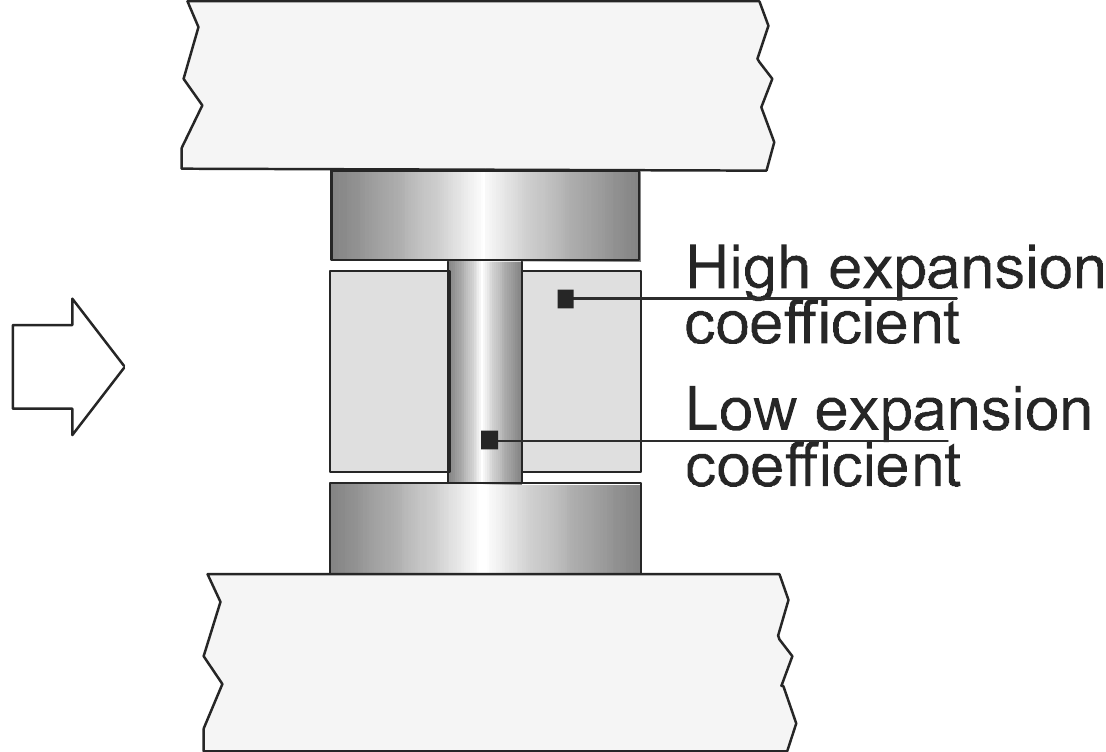
\includegraphics[height=0.18\textwidth]{Media/tcs_switch_02.png}\label{fig:tcs_switch12}}
	\caption{Bi-metallic heat switch, \cite{ref_tcs_04}.}
	\label{fig:tcs_switch01}
\end{figure}

\begin{figure}[H]
	\centering
	\subfloat[Comparison between data and theory (experimental results), \cite{ref_tcs_04} ]{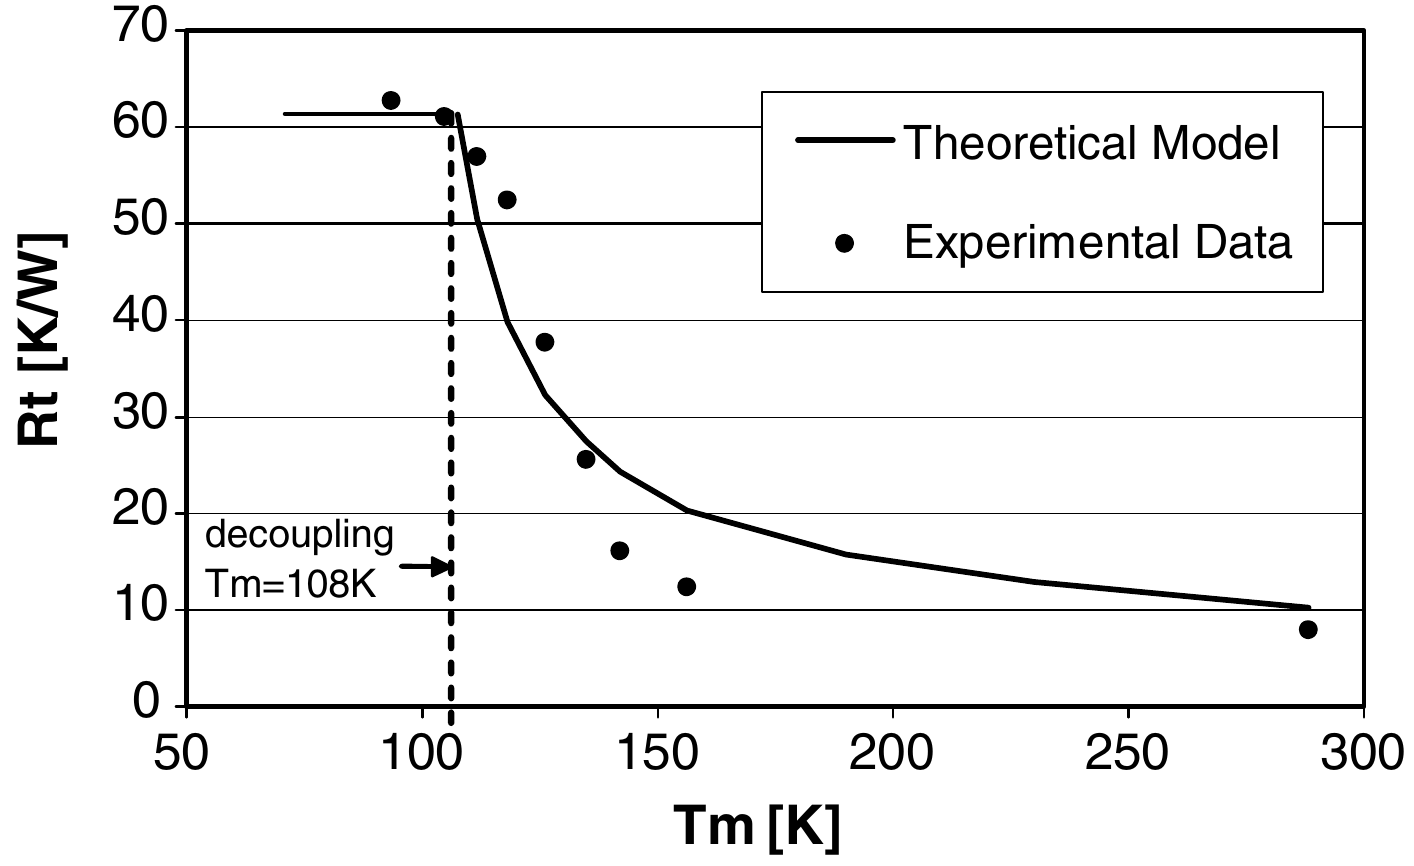
\includegraphics[height=0.22\textwidth]{Media/tcs_diag_orig.png}\label{fig:tcs_switch21}}\qquad
	\subfloat[Linearised characteristic of bi-metallic heat switch. ]{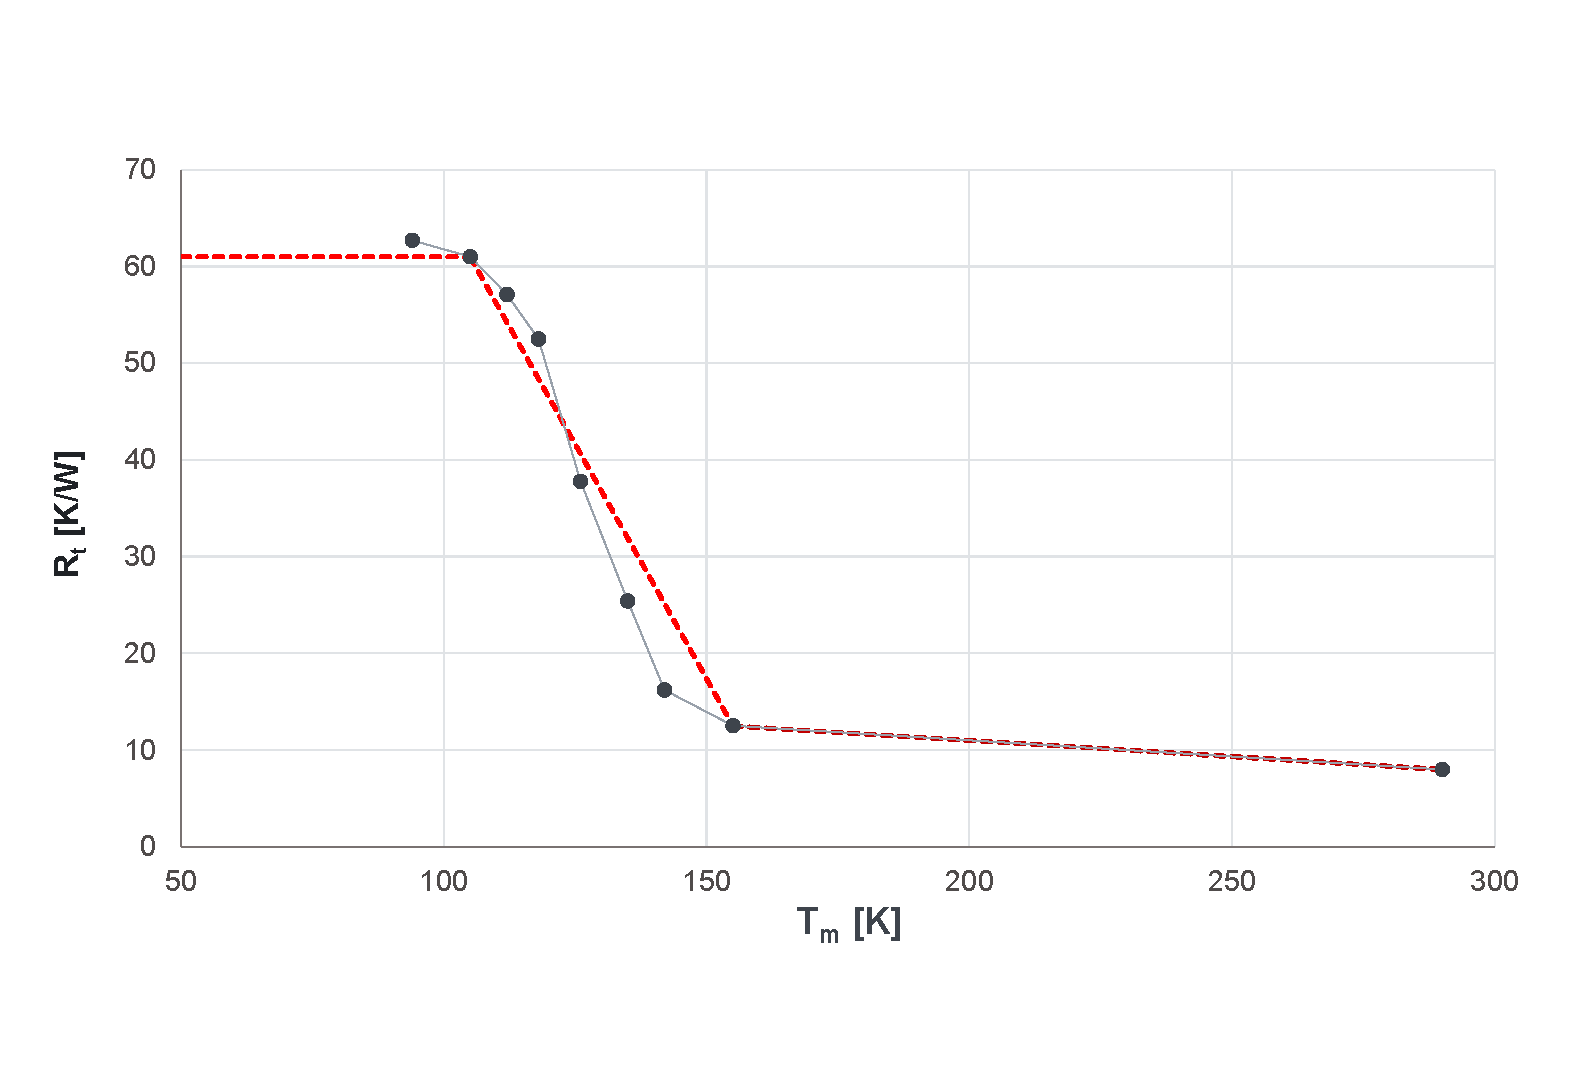
\includegraphics[height=0.22\textwidth]{Media/tcs_diag_lin}\label{fig:tcs_switch22}}
	\caption{Change of the heat switch conductivity $R_t$ over the mean temperature $T_M$.}
	\label{fig:tcs_switch02}
\end{figure}

\subsection{Thermal Network}
A thermal analysis was performed in order to get
\begin{itemize}
	\item the dimension of the insulation and heat straps,
	\item the necessary amount of RHUs and heat switches,
	\item the required surface finishing and
	\item the suitable choice of material.\\
\end{itemize}

For that, a thermal network with ten nodes was derived from the rover, shown in \autoref{fig:tcs_network}.
At the intersection of the steering and drive engien, two additional nodes were defined to calculate the heat flow.

\begin{figure}[h]
	\centering
	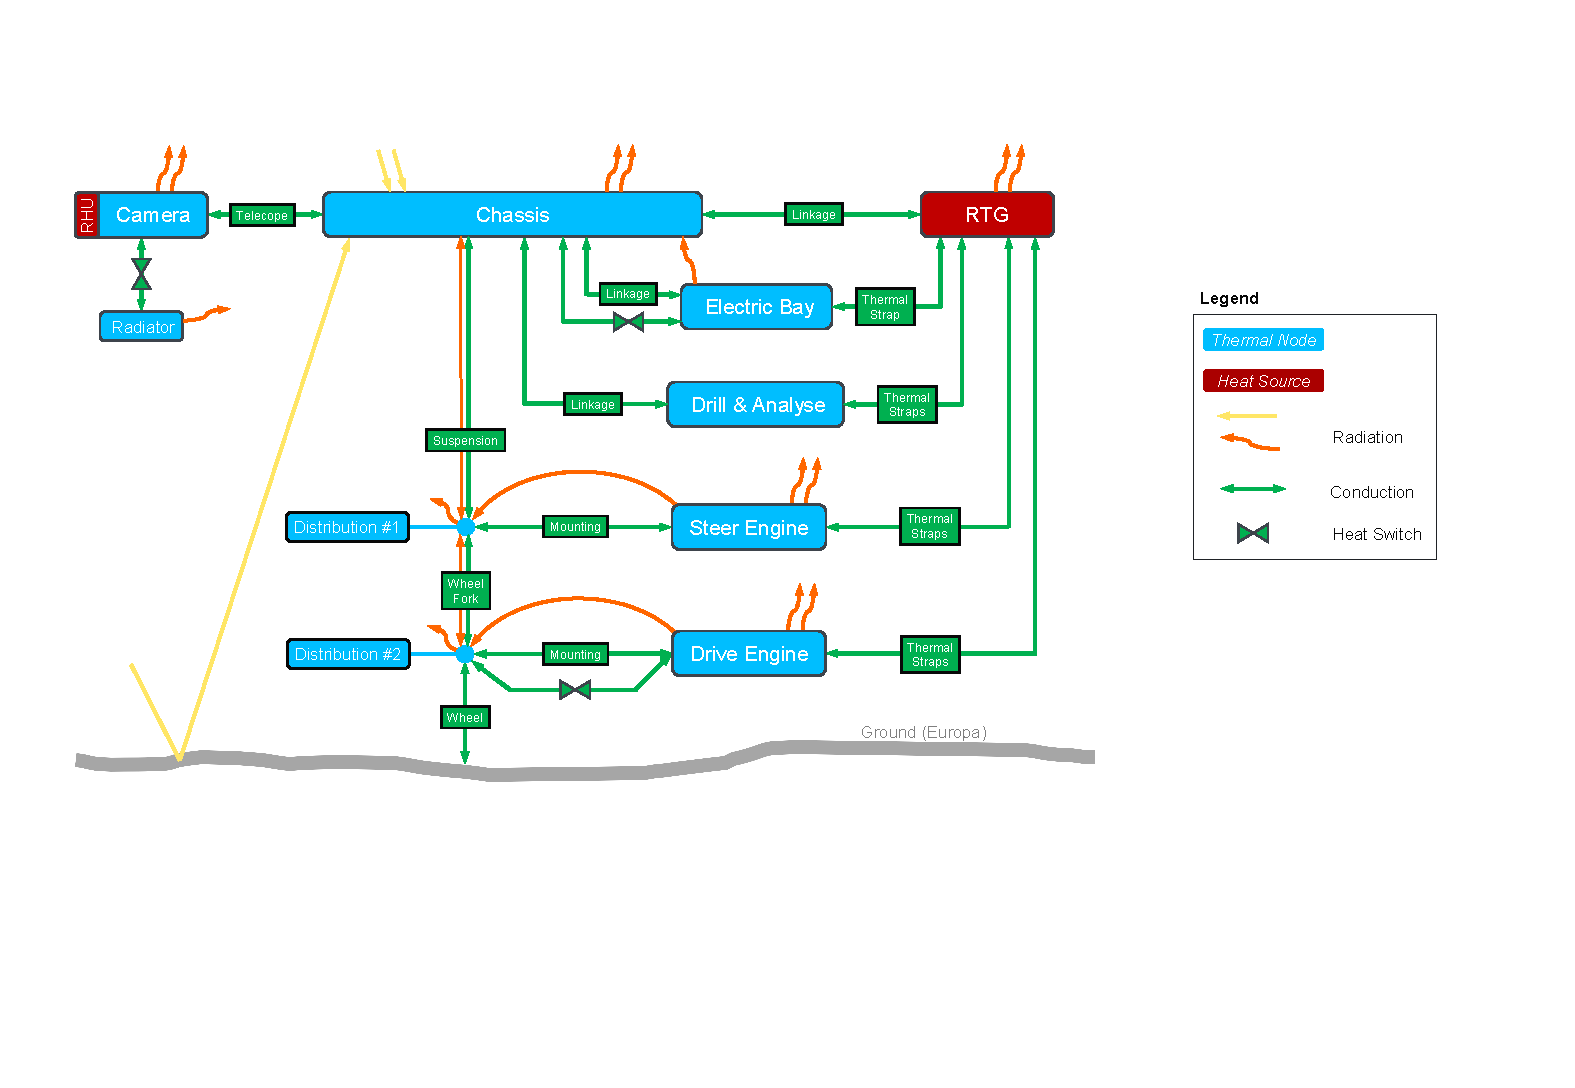
\includegraphics[width=0.85\textwidth]{Media/tcs_network}
	\caption{Thermal network of the rover.}
	\label{fig:tcs_network}
\end{figure}

On the basis of the thermal network, the heat energy equlibrium for each node was defined (see \appref{sec:app_tcs_01}).
The calculation were considered as a quasi-static analysis, were the component temperatures stay constant, $\frac{\dd T}{\dd t}=0$.
Due to the early state of the rover, simplifications and asumptions for the analysis were made.
\begin{itemize}
	\item The convection was neglected due to the thin atmosphere.
	\item The whole electrical power of the components will be dissipated into heat.
	\item A variation of $\pm 20\%$ for the emisivity and absorpsivity values was considered, if applicable (seet \autoref{tab:tcs_surface}).
	\item The heat as a result of retardation radiation inside the shielding was neglected.
	\item No dicrete nodes for the radar, hazcams, APXS and deployment engines were considered. Their heat will be lead into the chassis.
	\item The mechanism engines weren't considered.
	\item A half of bogies radiation loss were put to the chassis and Node 1 each. 
	\item A half of wheel forks radiation loss were put to the Node 1 and Node 2 each. 
\end{itemize}


\subsection{Analysis}
The thermal analysis was perfomred as an Excel calculation with the  possibility to adapt input values and dimension, \autoref{app:DigitalAppendix} Nr. 1.
The major driving load cases are the  hot and the cold cases, where the maximum and minimum temperatures of the rover components will be reached.
For that, the most powerful components were set to operating mode at once or only the minium requred components were turned on, respectively.
The emisivity and absorptivity were adjusted to fulfil the cases.
There were further load cases defined to consider the  battery charging, the communication mode and the drill \& analyse operation.

\subsection{Results}
The resulting temperatures for each node for the hot and cold cases  are listed in \autoref{tab:tcs_temp}.
The temperature margins for uncertainties, acceptance tests and qulification tests were considered with 5 K each, $\pm$15 K in total, \cite{ref_tcs_05}.
The corresponding temperatures are listed in \autoref{tab:tcs_temp1}.
All temperature lay betwenn their limits without using a heater.
Considering the temperature margin, the electric ebay exceeds the temperature limits of the transmitter, \autoref{tab:tcs_temp2}.
The issue can be solved by optimising the heat paths and adding furhter insulation during the detailed ebay design process.
Yet another results can be found in \autoref{tab:tcs_nodes1} to \autoref{tab:tcs_nodes5}, \autoref{tab:tcs_toggle} and  \autoref{tab:tcs_lynx}.


%-------------------------------------------------------------------------------
\section{Radiation} \label{sec:Radiation}
%-------------------------------------------------------------------------------

Compared to the radiation environment near Earth the radiation environment near Jupiter is multiple times stronger. It has the highest radiation levels of any planet in our solar systems \cite{Platzhalter}. In order to survive these harsh environmental conditions, special emphasis must be placed on the radiation protection. In \autoref{fig:trappedprotonelectronfluxes}, the average trapped proton and electron fluxes on Europa's orbit around Jupiter are shown in comparison to the outer Van Allen radiation belt around Earth. However, in contrast to the Van Allen radiation belt, the duration within the radiation environment on Europa cannot be minimised and the rover has to be designed to withstand the entire mission duration of 30 days. \\ \\
In oder to design and evaluate different radiation protection approaches, different calculations have to be performed. For this purpose the ESA SPace ENVironment Information System (SPENVIS) is used \cite{Platzhalter}. All calculations and figures in \autoref{sec:Radiation} are performed with SPENVIS unless otherwise stated.

\subsection{Radiation Protection}

\label{subsec:RadiationProtection}

Various options are available to protect the rover against the radiation. A common approach is the use of aluminium or titanium as these materials can also act as structural elements. However, due to the mass constraints of 30 kg other materials or material compositions are taken in consideration which are more mass effective. In \autoref{tab:OptimalRadiationProtection}, an optimised shield structure is presented for different weight thresholds designed for the radiation environment around Jupiter.

\begin{wraptable}{r}{8cm}
\centering
\caption{Optimal shield structure for an Jupiter mission. \cite{Platzhalter}}
\begin{adjustbox}{max width=\textwidth}
\begin{tabular}[l]{cccccc}

	\toprule
	
	Areal Density	&	\(0.5\)	&	\(1\) &  \(2\) & \(3\)	\\
	/ \(\text{g/cm}^2\)	&	&	&  & \\
	
	\midrule
	
	
	Layer No. 1	&	Pb &  Pb & W	& Ta	\\
	/ mm	&	0.415 &  0.829 & 0.984	& 1.563	\\
	
	
	Layer No. 2	&	Fe	&  Mg &	Mg & Al \\
	/ mm	&	\(0.033\)	&  \(0.158\) &	\(0.540\) & \(0.399\) \\
	
	
	Layer No. 3 &	-	&  -	& - & Mg \\
	/ mm &	-	&  -	& - & \(0.150\) \\
	

	\bottomrule

\end{tabular}
\end{adjustbox}
\label{tab:OptimalRadiationProtection}
\end{wraptable}

The difference between an aluminium or titanium shielding and an optimised structure listed in \autoref{tab:OptimalRadiationProtection} for the total ionizing dose (TID) is shown in \autoref{fig:AluminiumTitanOptimised}. \\ \\
Due to the mass savings of the optimised structure it will be used where the radiation protection of the aluminium structure is not sufficient. In order to reduce the mass further, a radiation vault is utilised that highly sensible components do not have to be shielded separately.

\subsection{Components}

\label{subsec:RadiationComponents}

Every component on the rover has a different radiation tolerance and therefore have to be placed at different compartments within the rover. The radiation tolerances are listed in \autoref{tab:RadiationList}. None sensitive components like the electric motors and harness are only shielded by an aluminium structure where components like the metal within the wire are resistant against the radiation. However, isolators around the cables have to be selected to be resistant in order to prevent short circuits. Highly sensitive components like cameras have an additional protective layer in order to reduce the TID to under 30 krad. Components which are within the rover like the on-board computer (OBC) are placed within the radiation vault which reduces the TID to under 20 krad. For this purpose the optimised shield structure with a weight target of 0.5 \(\text{g/cm}^2\) is used. Detailed TIDs for all components are shown in \autoref{fig:CompartmentTID}.

\subsection{Improvements}

\label{subsec:RadiationImprovements}

Even though the radiation protection is sufficient for the rover to survive at least the nominal mission of 30 days, further improvements can be performed in order to extend the secondary mission. \\ \\
Local shielding can be applied on less resistant components in order to reduce the wall thickness of the whole radiation wall. If components with a radiation tolerance under 43.27 krad are individually shielded a mass saving of 736.2 g can be achieved. Additionally, water ice extracted from the surface of Europa can be used to improve the radiation protection. With a layer of one centimetre of water, the TID within the radiation vault can be reduced to 16.03 krad without the additional radiation protection beside the 4 mm of aluminium structure. The start mass of the rover can therefore be reduced by 897.2 g by removing the additional shielding. \\ \\
Detailed calculations for local shielding and water improvements can be found in \apprefsub{app:AppendixRadiationImprovements} and may be analysed further in Phase B.

\subsection{Conclusion}

\label{subsec:RadiationConclusion}

In order to protect the rover against the high radiation levels at the surface of Europa, the rover has different compartments. High sensible components are placed within a radiation vault which has a mass optimised structure. Components which has to be outside the radiation vault but are highly sensible are shielded individually. Low sensible Components are protected by the Aluminium structure. \autoref{fig:RadiationOverview} illustrates the different compartments within the rover and the accorded TIDs.

\begin{figure}[htb]
     \centering
     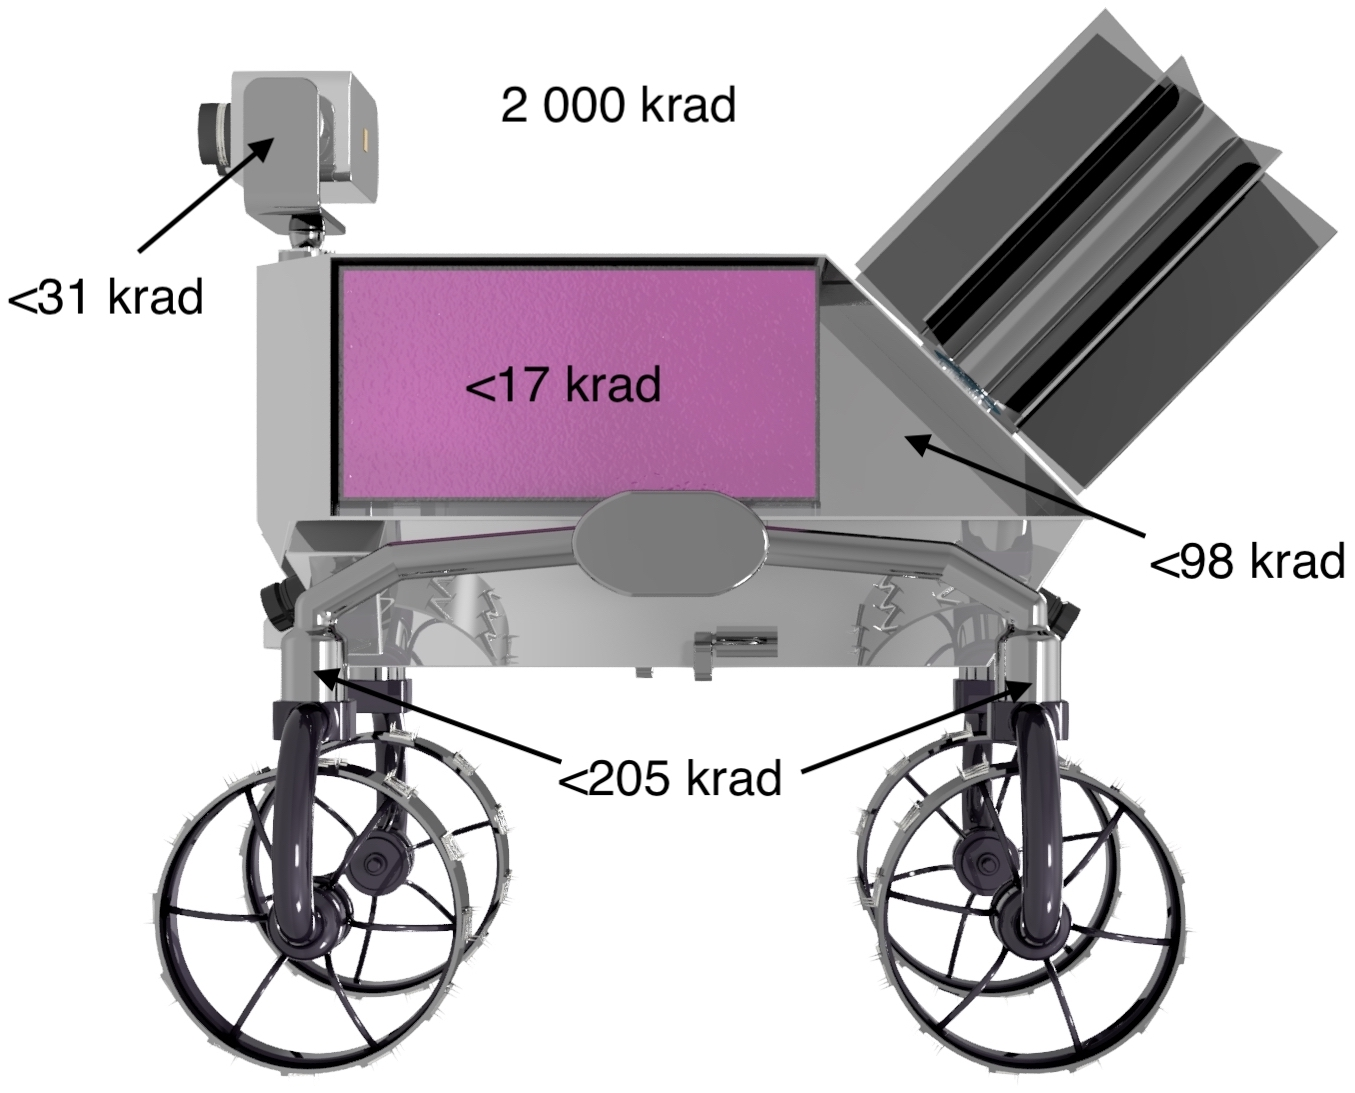
\includegraphics[width=\textwidth]{Media/INSPIRE_Radiation}
     \caption{Overview of TIDs within different compartments within the rover.}
     \label{fig:RadiationOverview}
\end{figure}

\clearpage
\chapter{Outlook \& Risk Assessment}
\label{chap:outlook}

\section{Risk Assessment}
\label{sec:RiskAssessment}

To reduce risks and increase the robustness within the development process for the INSPIRE mission, all subsystems focus on flight proven or space grade hard ware. \autoref{tab:SubSys-TRL} provides an overview on the resulting TRL for each subsystem. 
 
\begin{table}[h]
\centering
\caption{Subsystem TRL for risk assessment}
\begin{tabular}{llll}
\toprule
Subsystem            & overall TRL & Deviating component      &  \\
\midrule
Payload              & 0           & Drill System and Sample Analyser TRL 0 &  \\
Structure \& Mechan. & 0           & Boom Mechanism TRL 0     &  \\
Locomotion           & 9           & Structure Components for Locomotion TRL 0                     &  \\
EPS                  & 9           & PCDU may be customized                     &  \\
TCS                  & 9           & none                     &  \\
COMs, C\&DH          & 9           & Housekeeping TRL 0       & 	 \\
\bottomrule
\end{tabular}
\label{tab:SubSys-TRL}
\end{table}

Housekeeping electronics and the Boom Mechanism to extend the camera head for the INSPIRE mission will be custom designed components and therefore rated at TRL 0. However due to proven development processes and simple testing the risk for the mission progress is rated non critical.  \\

Payload components development depict the highest risk for the mission. The Analyser for the ice core samples is a downsized replica of the [missing reference]. 
The ice core drill derives from the Nano Drill offered by Honeybee Robotics [Missing reference]. Although the technology is available, the drill has to be adapted and tested. Testing in analog conditions potentially takes place in the arctic region and therefore lengthen the mission development process. \\

As a conclusion the payload subsystem development contains the highest risk for the INSPIRE mission. However the risk is considered manageable. Additionally investing in payload development is regarded worth the risk taking as it is integral to the successful investigation of Europa.

For the TCS the dimension of the  bi-metallic heat switches has to be adapted.
Tests in a special environment and for qualification have to be done as well. 

\clearpage

\section{Outlook}
\label{sec:Outlook}

In the further design iterations, detailed simulations of the chassis and the running gear could be carried out in order to get a better understanding of where the problems of the system are and at which points mass can possibly be reduced or should be added. It could also be considered whether a less complex mechanism for unfolding the drill can be found / designed. \\

Currently, the ice core samples taken be discarded after the analysis. It could be debated whether these samples will continue to be used. The previous considerations on this topic were, on the one hand, to store the samples and bring them back to the lander in order to be able to carry out further analyzes if the lander should have a gripper arm or something similar to receive the samples or, on the other hand, to melt the samples and transport them to the Electric Bay with the help of micropumps in order to use the water gained in this way as protection against radiation. This could serve as a replacement for the previous solution and in the best case even save mass. \\

For the TCS, a more detailed analysis should to be carried out with the Finite-Element-Method to calculate the local heat and temperature distribution.
The FE results could be used to verify and adjust the analytical analysis to get a helpful tool for fast thermal calculation to evaluate different materials or desings in the further development phases.

\clearpage


%Quellenverzeichnis über Citavi Anbindung
%###########################################################################
%
%   Literaturverzeichnis
%
%###########################################################################


%\begin{thebibliography}{99}
%\addcontentsline{toc}{chapter}{References}
%
%%###########################################################################
%% Eintrag durch \bibitem[marke]{bezug} eintrag_text
%
%% Motivation

%\bibliography{REF}

\printbibliography

\addcontentsline{toc}{chapter}{\bibname}

%###########################################################################
%
% Anhang
%
%###########################################################################
%\begin{appendix}
%\label{chap:Appendix}
%\chapter{Appendix A}
%\setcounter{chapter}{1}
%\addcontentsline{toc}{chapter}{Appendix}
%###########################################################################
% Anhang A
%###########################################################################
%\label{A}
%....


%\chapter{Appendix B}
%###########################################################################
% Anhang B
%###########################################################################
%\label{B}

%\pagebreak
%###########################################################################
%\end{appendix}


\renewcommand\thesection{\Alph{section}}
\renewcommand\thefigure{\thesection.\arabic{figure}}
\renewcommand{\thetable}{\thesection.\arabic{table}}
\setcounter{figure}{0}
\setcounter{table}{0}
\setcounter{section}{0}

\chapter*{Appendix}
\addcontentsline{toc}{chapter}{Appendix}

\label{chap:Appendix}

\section{Operation}


% Please add the following required packages to your document preamble:
% \usepackage{graphicx}
% \usepackage[table,xcdraw]{xcolor}
% If you use beamer only pass "xcolor=table" option, i.e. \documentclass[xcolor=table]{beamer}
\begin{table}[hbt]
\centering
\resizebox{0.7\textwidth}{!}{%
\begin{tabular}{|c|c|c|l|}
\hline
Number & Rover System Modes                  & Abbrevation & \multicolumn{1}{c|}{Definition}                                                                                                                                                                                                                                                                                                                                                                                                                                                                                                                                                                                                   \\ \hline
\rowcolor[HTML]{EFEFEF} 
0      & Launch/Off Mode                     & OFF         & \begin{tabular}[c]{@{}l@{}}From Launch until EDL Phase\\ Rover System is OFF\\ Exact mode description t.b.d. and can be adapted to meet the lander demands\\ Health tests on Occasion during flight time are foreseen (PCDU could be active)\\ Batteries on Storage Capacity at launch and may be recharged on occasion (like Rosetta Mission)\\ Telemetry data shall be sent by the Lander (optional if possible)   \\ RTG on =\textgreater Electrical and Thermal Power may be used \\ (for Lander Power and Thermal Systems) or is disposed of by shunts\end{tabular}                                                          \\ \hline
\rowcolor[HTML]{EFEFEF} 
1      & Entry, Descent and Landing          & EDL         & \begin{tabular}[c]{@{}l@{}}From Entry until next morning after secure landing of Lander on Europa\\ See Mode OFF\\ PCDU ON after secure landing (Powered by RTG)\\ Heaters ON (powered by remaining RTG Power)\\ Battery charging if no Kill Switch is used\end{tabular}                                                                                                                                                                                                                                                                                                                                                          \\ \hline
\rowcolor[HTML]{EFEFEF} 
2      & Deployment and Early Operation Mode & EOP         & \begin{tabular}[c]{@{}l@{}}First Morning after EDL\\ Exact mode description t.b.d. and can be customized to lander \\ =\textgreater Dependant on final Lander Design\\ Critical Deployments (Egress System) and leaving the lander\\ Optional whether Kill Switch ejected =\textgreater Battery charging can start\\ Rover System Activation possibilities: Kill Switch, Lander Interface, HPC from Earth\\ PCDU ON\\ OBC ON\\ Heaters ON\\ After sufficient Battery Capacity is reached (50\%): Deployment of Rover Boogie \\ and checkout/health check of all Rover Systems\\ Afterward switching to Charging Mode\end{tabular} \\ \hline
3      & Idle/ Perception                    & ID          & \begin{tabular}[c]{@{}l@{}}During Idle Operation Time\\ Rover powered by RTG or Batteries (Excess Power charges Batteries)\\ PCDU ON\\ All Components in Standby or Power Saving Mode if possible\\ Stereovision Camera ON for Orientation and Observation (Science Data)\\ Hazcams and OBC ON for Orientation and Path Analysation\\ COMM ON for larger time intervals (Listening Mode)\end{tabular}                                                                                                                                                                                                                             \\ \hline
4      & Safe Mode/ Hibernation (SAFE)       & SAFE        & \begin{tabular}[c]{@{}l@{}}Entered in case of emergency or contingency Rover    \\ Survival Mode =\textgreater Minimum Power\\ PCDU ON  \\ COMM sends Emergency Signal then switches to\\ COMM ON for small time intervals (Listening Mode)\\ OBC OFF until Command received =\textgreater High Power Commands (HPC)\\ Heaters ON\\ Science data shall be stored without data loss\\ Applicable during Day and Nighttime\\ Exit after receiving the corresponding command\\ (Optional: Timer ON and Restart of Rover System after time period has passed)\end{tabular}                                                            \\ \hline
6      & Communication                       & COMM        & \begin{tabular}[c]{@{}l@{}}During Transmission of major Telemetry or Science Data\\ Rover powered by RTG or Batteries (Excess Power charges Batteries)\\ PCDU ON\\ All Components in Standby or Power Saving Mode if possible\\ OBC SB\\ COMM ON (Transmission Mode)\end{tabular}                                                                                                                                                                                                                                                                                                                                                 \\ \hline
7      & Charging                            & BAT         & \begin{tabular}[c]{@{}l@{}}For Battery charging\\ Rover batteries charged by RTG\\ PCDU ON\\ All Components in Standby or Power Saving Mode if possible\\ OBC SB\\ Quit after sufficient charge is reached\end{tabular}                                                                                                                                                                                                                                                                                                                                                                                                           \\ \hline
8      & Locomotion                          & LOC         & \begin{tabular}[c]{@{}l@{}}For Rover Movement and Observation\\ Locomotion and Navigation ON\\ Hazcams and Traversing Path Analysis ON\\ OBC ON\\ PCDU ON\\ COMM OFF\\ Stereovision Camera ON for Orientation and Observation (Science Data)\\ Only during Daytime\end{tabular}                                                                                                                                                                                                                                                                                                                                                   \\ \hline
9      & Payload Observation Mode            & OBS         & \begin{tabular}[c]{@{}l@{}}Payload Mode for Science Data Collection during Daytime\\ OBC ON\\ PCDU ON   \\ COMM OFF\\ Stereovision Camera ON for Orientation and Observation (Science Data)\\ RADAR ON for Ground Investigation =\textgreater Drill Location\\ Only during Daytime\end{tabular}                                                                                                                                                                                                                                                                                                                                   \\ \hline
10     & Payload: Ice Core Mode              & ICE         & \begin{tabular}[c]{@{}l@{}}Payload Mode for   Science Data Collection during Daytime or Nighttime\\ OBC ON\\ PCDU ON\\ COMM OFF\\ Ice Core Drill ON during Ice   Core Sample Collection\\ Afterwards Sample will be   analysed =\textgreater APXS ON\end{tabular}                                                                                                                                                                                                                                                                                                                                                                 \\ \hline
\end{tabular}%
}
\caption{Collection of Rover System Modes.}
\label{tab:systemmod}
\end{table}

\clearpage

%-------------------------------------------------
\section{Structure and Mechanism} \label{sec:AppendixStructureandMechanism}
%-------------------------------------------------

% Please add the following required packages to your document preamble:
% \usepackage{booktabs}
% \usepackage{multirow}
% \usepackage{graphicx}
\begin{table}[hbt]
\centering
\caption{INSPIRE Mass Budget}
\resizebox{\textwidth}{!}{%
\begin{tabular}{@{}cccccc@{}}
\toprule
Subsystem                               & component name                      & mass per component {[}kg{]} & quantity & component margin & total {[}kg{]} \\ \midrule
\multirow{5}{*}{Structure \& Mechanism} & Harness                             & 3                           & 1        & 20\%             & 3,60           \\
                                        & Chassi                              & look up at Chassi Table     & 1        & 20\%             & 5,02           \\
                                        & E-Bay Box                           & 1,033                       & 1        & 20\%             & 1,24           \\
                                        & Boom                                & 0,17                        & 1        & 20\%             & 0,20           \\
                                        & Solar Cell Plate                    & 0,121                       & 1        & 20\%             & 0,15           \\ \midrule
\multirow{7}{*}{Locomotion}             & wheels                              & 0,158                       & 4        & 20\%             & 0,76           \\
                                        & rims                                & 0,162                       & 4        & 20\%             & 0,78           \\
                                        & motor (wheels)                      & 0,057                       & 4        & 10\%             & 0,25           \\
                                        & planetary gear(wheels)              & 0,118                       & 4        & 10\%             & 0,52           \\
                                        & Motor (steering)                    & 0,07                        & 4        & 5\%              & 0,29           \\
                                        & Motor (deployment)                  & 0,07                        & 6        & 5\%              & 0,44           \\
                                        & IMU                                 & 0,012                       & 4        & 10\%             & 0,05           \\ \midrule
\multirow{4}{*}{EPS}                    & Battery                             & 1,98                        & 1        & 10\%             & 2,18           \\
                                        & RTG                                 & 3,5                         & 1        & 10\%             & 3,85           \\
                                        & SolarCells                          & 0,0012975                   & 10       & 20\%             & 0,02           \\
                                        & PCDU                                & 0,33                        & 1        & 20\%             & 0,40           \\ \midrule
\multirow{4}{*}{Communication}          & LGAs                                & 0,002                       & 4        & 5\%              & 0,01           \\ 
                                        & Transmitter                         & 0,195                       & 2        & 5\%              & 0,41           \\
                                        & Receiver                            & 0,22                        & 2        & 10\%             & 0,48           \\
                                        & Multiplexer                         & 0,065                       & 2        & 5\%              & 0,14           \\\midrule
\multirow{4}{*}{C\&DH / sensors}        & Sun Sensors                         & 0,016                       & 4        & 5\%              & 0,07           \\
                                        & OBC                                 & 0,35                        & 2        & 5\%              & 0,74           \\
                                        & temperature Sensor                  & 0,0002                      & 20       & 20\%             & 0,00           \\
                                        & Housekeeping                        & 0,2                         & 1        & 5\%              & 0,21           \\ \midrule
\multirow{5}{*}{Thermal Control System} & Heaters                             & 0,00181                     & 10       & 5\%              & 0,002          \\
                                        & isolation                           & 0,07                        & 1        & 20\%             & 0,08           \\
                                        & Carbon Straps                       & 0,48                        & 1        & 5\%              & 0,5            \\
                                        & RHU                                 & 0,3                         & 1        & 5\%              & 0,32           \\
                                        & Bi-metallic Heat Switch             & 0,06                        & 10       & 10\%             & 0,66           \\ \midrule
\multirow{10}{*}{Payload}               & Ice Core Drill Motor \& Electronics & 1,3                         & 1        & 20\%             & 1,56           \\
                                        & Ice Core Drill Titanium bit         & 0,041                       & 1        & 20\%             & 0,05           \\
                                        & Groundradar electronics             & 0,045                       & 1        & 5\%              & 0,05           \\
                                        & Ground Radar antenna                & 0,00273                     & 2        & 10\%             & 0,01           \\
                                        & APXS Analyzer                       & 0,43                        & 1        & 20\%             & 0,52           \\
                                        & Haz Cams                            & 0,064                       & 3        & 5\%              & 0,20           \\
                                        & Stereo Vision Cam                   & 0,064                       & 2        & 5\%              & 0,13           \\
                                        & objective StereoCam                 & 0,08                        & 2        & 20\%             & 0,19           \\
                                        & objective HazCam                    & 0,048                       & 3        & 20\%             & 0,17           \\
                                        & LEDs                                & 0,003                       & 16       & 10\%             & 0,05           \\ \midrule
\multirow{2}{*}{Radiation}              & Cam shielding                       & 0,02905                     & 5        & 20\%             & 0,17           \\
                                        & E-Bay shielding                     & 0,94                        & 1        & 20\%             & 1,13           \\ \midrule
\multicolumn{5}{c}{Mass incl. Component Margins}                                                                                          & 27,25          \\
\multicolumn{5}{c}{System Margin}                                                                                                         & 10\%         \\
\multicolumn{5}{c}{Total Mass of INSPIRE}                                                                                                 & 29,97        \\\bottomrule
\end{tabular}%
}
\label{tab:totalMass}
\end{table}

\clearpage

% Please add the following required packages to your document preamble:
% \usepackage{booktabs}
% \usepackage{graphicx}
\begin{table}[hbt]
\centering
\caption{INSPIRE Chassi Mass Budget}
\resizebox{\textwidth}{!}             & \multicolumn{1}{c}{0,27}           \\
\multicolumn{2}{c}{CamHead  Fork}                    & \multicolumn{1}{c}{0,119}                        & \multicolumn{1}{c}{1}        & \multicolumn{1}{c}{20\%}             & \multicolumn{1}{c}{0,14}           \\
\multicolumn{2}{c}{Frontplate}                       & \multicolumn{1}{c}{0,165}                        & \multicolumn{1}{c}{1}        & \multicolumn{1}{c}{20\%}             & \multicolumn{1}{c}{0,20}           \\
\multicolumn{2}{c}{Sideplate}                        & \multicolumn{1}{c}{0,244}                        & \multicolumn{1}{c}{2}        & \multicolumn{1}{c}{20\%}             & \multicolumn{1}{c}{0,59}           \\
\multicolumn{2}{c}{Backplate}                        & \multicolumn{1}{c}{0,16}                         & \multicolumn{1}{c}{1}        & \multicolumn{1}{c}{20\%}             & \multicolumn{1}{c}{0,19}           \\
\multicolumn{2}{c}{Topplate}                         & \multicolumn{1}{c}{0,32}                         & \multicolumn{1}{c}{1}        & \multicolumn{1}{c}{20\%}             & \multicolumn{1}{c}{0,38}           \\
\multicolumn{2}{c}{Drillingbay}                      & \multicolumn{1}{c}{0,433}                        & \multicolumn{1}{c}{1}        & \multicolumn{1}{c}{20\%}             & \multicolumn{1}{c}{0,52}           \\
\multicolumn{2}{c}{Midplate}                         & \multicolumn{1}{c}{0,491}                        & \multicolumn{1}{c}{1}        & \multicolumn{1}{c}{20\%}             & \multicolumn{1}{c}{0,59}           \\
\multicolumn{2}{c}{Differential}                     & \multicolumn{1}{c}{0,237}                        & \multicolumn{1}{c}{1}        & \multicolumn{1}{c}{20\%}             & \multicolumn{1}{c}{0,28}           \\
\multicolumn{2}{c}{Faulhaber Motor}                  & \multicolumn{1}{c}{0,015}                        & \multicolumn{1}{c}{4}        & \multicolumn{1}{c}{20\%}             & \multicolumn{1}{c}{0,07}           \\
\multicolumn{2}{c}{IceCoreDeployment Housing}        & \multicolumn{1}{c}{0,005}                        & \multicolumn{1}{c}{4}        & \multicolumn{1}{c}{20\%}             & \multicolumn{1}{c}{0,02}           \\
\multicolumn{2}{c}{Trapdoor}                         & \multicolumn{1}{c}{0,047}                        & \multicolumn{1}{c}{2}        & \multicolumn{1}{c}{20\%}             & \multicolumn{1}{c}{0,11}           \\
\multicolumn{2}{c}{DrillFork1}                       & \multicolumn{1}{c}{0,011}                        & \multicolumn{1}{c}{1}        & \multicolumn{1}{c}{20\%}             & \multicolumn{1}{c}{0,01}           \\
\multicolumn{2}{c}{DrillFork2}                       & \multicolumn{1}{c}{0,017}                        & \multicolumn{1}{c}{1}        & \multicolumn{1}{c}{20\%}             & \multicolumn{1}{c}{0,02}           \\
\multicolumn{2}{c}{Wheel  Fork}                      & \multicolumn{1}{c}{0,122}                        & \multicolumn{1}{c}{4}        & \multicolumn{1}{c}{20\%}             & \multicolumn{1}{c}{0,59}           \\
\multicolumn{2}{c}{Gear  \& Motor Housing (Driving)} & \multicolumn{1}{c}{0,015}                        & \multicolumn{1}{c}{4}        & \multicolumn{1}{c}{20\%}             & \multicolumn{1}{c}{0,07}           \\
\multicolumn{2}{c}{Deployment  Mechanism Housing}    & \multicolumn{1}{c}{0,118}                        & \multicolumn{1}{c}{2}        & \multicolumn{1}{c}{20\%}             & \multicolumn{1}{c}{0,28}           \\
\multicolumn{2}{c}{Bogie}                            & \multicolumn{1}{c}{0,11}                         & \multicolumn{1}{c}{4}        & \multicolumn{1}{c}{20\%}             & \multicolumn{1}{c}{0,53}           \\
\multicolumn{2}{c}{HazCamBox\_Front}                 & \multicolumn{1}{c}{0,046}                        & \multicolumn{1}{c}{2}        & \multicolumn{1}{c}{20\%}             & \multicolumn{1}{c}{0,11}           \\
\multicolumn{2}{c}{HazCamBox\_Heck}                  & \multicolumn{1}{c}{0,027}                        & \multicolumn{1}{c}{1}        & \multicolumn{1}{c}{20\%}             & \multicolumn{1}{c}{0,03}           \\
\multicolumn{2}{c}{GroundRadarAntenna  holder}       & \multicolumn{1}{c}{0,03}                         & \multicolumn{1}{c}{1}        & \multicolumn{1}{c}{20\%}             & \multicolumn{1}{c}{0,04}           \\ \midrule
\multicolumn{5}{c}{Mass with component margins}                                                                                                                               & \multicolumn{1}{c}{5,02}           \\
\multicolumn{5}{c}{System Margin}                                                                                                                                             & \multicolumn{1}{c}{10\%}           \\
\multicolumn{5}{c}{Total Mass}                                                                                                                                                & \multicolumn{1}{c}{5,52}           \\\bottomrule
\end{tabular}%
}
\label{tab:ChassiBudget}
\end{table}




\clearpage

\setcounter{figure}{0}
\setcounter{table}{0}

%-------------------------------------------------
\section{Locomotion} 
\label{app:Loco}
%-------------------------------------------------

\subsection{Locomotion Design Drivers}
\label{app:DesignDrivers}

In this section all necessary values for the design of the locomotion system are presented.   


\begin{figure}[htb]
{\centering
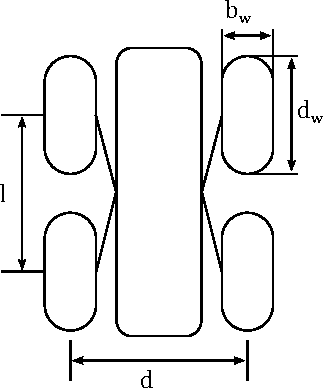
\includegraphics[width=0.7\textwidth]{Media/Geometries}
\caption{Geometric dimensions for the locomotion system.}
\label{fig:Ackerman}
}
\end{figure}

 
     
\begin{table}[htb]
     \centering
     \caption{Soil parameters for both soils considered: heav clay as hard equivalent for ice values and snow in Sweden \cite{Bekker}.}
     \begin{adjustbox}{max width=\textwidth}
     \begin{tabular}[l]{lcccccc}
     
     	\toprule
     		\multicolumn{1}{l}{Terrain} & \qquad \qquad	& \multicolumn{1}{c}{\(n\) /\(\frac{\text{kN}}{\text{m}^{n+1}}\)} & \multicolumn{1}{c}{\(k_\text{c}\)} & \multicolumn{1}{c}{\(k_\phi\) / \(\frac{\text{kN}}{\text{m}^{n+2}}\)} & \multicolumn{1}{c}{\(c\) /kPa} & \multicolumn{1}{c}{\(\phi\) /deg}  \\
      
       	\midrule
 
     Heavy Clay		&	&	0.13	&	12.70	&	1555.95		&	68.95	&	34			\\	
     Snow (Sweden)	&	&	1.44	&	10.55	&	66.08		&	6		&	20.7		\\	

     	\bottomrule
     
     \end{tabular}
     \end{adjustbox}
     \label{tab:SoilParam}
     \end{table}     


\begin{table}[htb]
\centering
\caption{Various wheel dimensions respective to the weight. Highlighted fields in red are not considered further for system design due to the limit of 200 g weight per wheel.}
\begin{adjustbox}{max width=\textwidth}
\begin{tabular}[l]{lcc|lcc}

	\toprule
		\multicolumn{1}{l}{Wheel Width} & \multicolumn{1}{c}{Wheel Diameter} & \multicolumn{1}{c|}{Weight per Wheel}	& \multicolumn{1}{l}{Wheel Width}	 & \multicolumn{1}{c}{Wheel Diameter} 		& \multicolumn{1}{c}{Weight per Wheel}    \\

\multicolumn{1}{l}{\:\:\:\:\:\: m}		& \multicolumn{1}{c}{m} 			& \multicolumn{1}{c|}{g} 					& \multicolumn{1}{l}{\:\:\:\:\:\: m}& \multicolumn{1}{c}{m}					& \multicolumn{1}{c}{g} \\
	\midrule
	
	0.05	&	0.1		&	127		& 0.05		&	0.15	&	185									\\ 
	0.06	&	0.1		&	153		&	0.06	&	0.15	&	\cellcolor[HTML]{CB0000}221		\\	
	0.07	&	0.1		&	178		&	0.07	&	0.15	&	\cellcolor[HTML]{CB0000}258		\\
	0.08	&	0.1		&	\cellcolor[HTML]{CB0000}204	&	0.08	&	0.15	&	\cellcolor[HTML]{CB0000}294		\\	
	0.09	&	0.1		&	\cellcolor[HTML]{CB0000}229	&	0.09	&	0.15	&	\cellcolor[HTML]{CB0000}331		\\
	0.1		&	0.1		&	\cellcolor[HTML]{CB0000}265	&	0.1		&	0.15	&	\cellcolor[HTML]{CB0000}367		\\	
	0.05	&	0.125	&	154		&	0.05	&	0.2		&	\cellcolor[HTML]{CB0000}236		\\
	0.06	&	0.125	&	185		&	0.06	&	0.2		&	\cellcolor[HTML]{CB0000}284		\\
	0.07	&	0.125	&	\cellcolor[HTML]{CB0000}217		&	0.07	&	0.2		&	\cellcolor[HTML]{CB0000}332		\\	
	0.08	&	0.125	&	\cellcolor[HTML]{CB0000}247		&	0.08	&	0.2		&	\cellcolor[HTML]{CB0000}379		\\
	0.09	&	0.125	&	\cellcolor[HTML]{CB0000}278		&	0.09	&	0.2		&	\cellcolor[HTML]{CB0000}427		\\
	0.1		&	0.125	&	\cellcolor[HTML]{CB0000}309		&	0.1		&	0.2		&	\cellcolor[HTML]{CB0000}487		\\
	
	\bottomrule

\end{tabular}
\end{adjustbox}
\label{tab:Geometry}
\end{table}


\subsubsection*{Mean Maximum Pressure}
\label{app:MMP}

To determine the mean maximum pressure, the data are taken from \autoref{fig:MMP_param}. 

\begin{figure}[htb] 
  \centering
     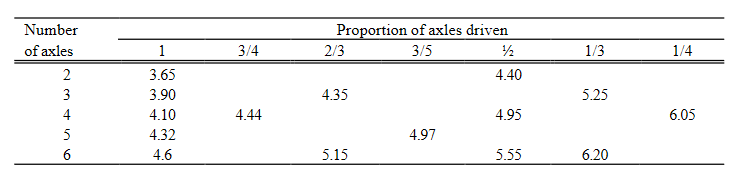
\includegraphics[width=1\textwidth]{Media/MMP_Param.png}
  \caption{Parameters for the mean maximum pressure for a wheeled rover.}
  \label{fig:MMP_param}
\end{figure}

The rover has 4 number ox axles, each with a quarter proportion of axles driven. Thus, the \(MMP\) can be calculated to:
\begin{equation}
	MMP \:  = \: \frac{K \cdot W}{2N{b_\text{w}}^{0.85}{d_\text{w}}^{1.15} { \left( \delta / d_\text{w} \right) }^{0.5}}		,
	\label{eq:MMP}
\end{equation}

with \(K = 6.05\) and the number of wheels \(N=4\). The resulting \(MMP\) for the 6 considered configurations are shown in \autoref{fig:MMP}. 

\begin{figure}[htb] 
  \centering
     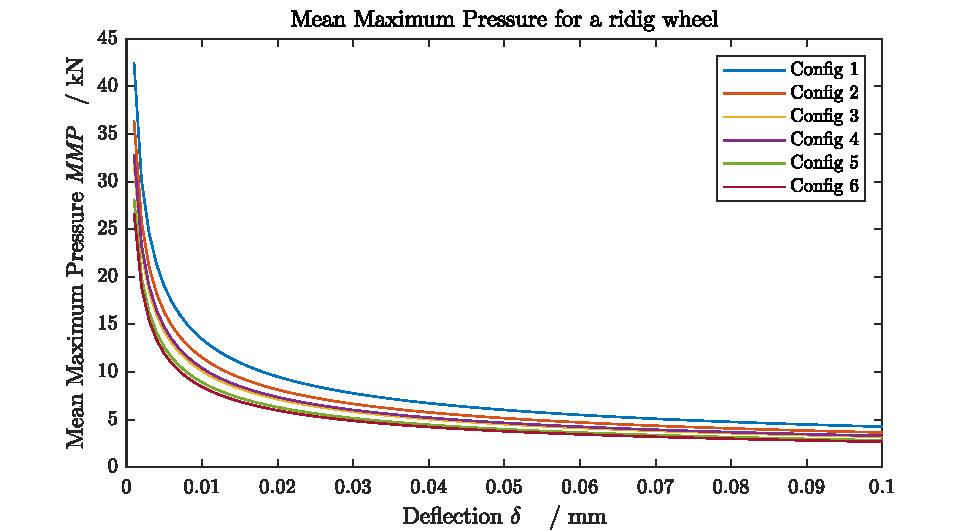
\includegraphics[width=1\textwidth]{Media/MMP for each Config.pdf}
  \caption{}
  \label{fig:MMP}
\end{figure}


\subsubsection*{Ackerman Steering}
\label{app:Ackerman}

As mentioned in \autoref{sec:Steering}, with Ackerman steering it is important to take into account that the angles of the front wheel positions differ: 

\begin{equation}
	\cot \theta_{i} - \cot \theta_\text{o} \:  = \:	- \frac{d}{l}	.
	\label{eq:Ackerman}
\end{equation}

With a wheel distance of \(d = 277\)~mm and \(l = 365\)~mm, the respective angles of the wheel positions can be determined. These values are necessary to control the drive in an autonomous drive mode.


\subsubsection*{Hardware Selection}
\label{app:Hardware}

Each wheel has a separate BLDC motor for driving. The necessary torque is listed for both soil parameters depending on the slope angle. In addition, necessary power is listed for different velocities to be reached, also for both soils. It should be noted, that the deflection \(\delta\) is not considered and assumed to be \(\delta = 0\).

\begin{table}[htb]
\centering
\caption{}
\begin{adjustbox}{max width=\textwidth}
\begin{tabular}[l]{lcccc|ccc}

	\toprule
		\multicolumn{1}{l}{\(\theta\)} & \multicolumn{1}{c}{\(R_\text{total,Snow}\)} & \multicolumn{1}{c}{\(\tau_\text{snow}\)} & \multicolumn{1}{c}{\(R_\text{total,HeavyClay}\)} & \multicolumn{1}{c|}{\(\tau_\text{HeavyClay}\)}	& \multicolumn{1}{c}{\(v\)}  & \multicolumn{1}{c}{\(P_\text{Min.,Snow}\)}  & \multicolumn{1}{c}{\(P_\text{Min.,HeavyClay}\)}			 \\
		
	\multicolumn{1}{l}{\:\:\:\:\:\: deg} & \multicolumn{1}{c}{N} & \multicolumn{1}{c}{Nm} & \multicolumn{1}{c}{N} & \multicolumn{1}{c|}{Nm} & \multicolumn{1}{c}{\(\frac{m}{s}\)} & \multicolumn{1}{c}{W} & \multicolumn{1}{c}{W} \\

	\midrule
		
	0	&	4.882	&	0.244	&	0.234	&	0.012	&	0.2		&	0.976	&	0.047	\\		
	7	&	6.040	&	0.302	&	1.436	&	0.072	&	0.35	&	2.114	&	0.503	\\
	14	&	7.094	&	0.355	&	2.618	&	0.131	&	0.5		&	3.547	&	1.309	\\
	21	&	8.028	&	0.401	&	3.765	&	0.188	&	0.65	&	5.219	&	2.447	\\
	28	&	8.833	&	0.442	&	4.857	&	0.243	&	0.8		&	7.067	&	3.886	\\
	35	&	9.499	&	0.475	&	5.880	&	0.294	&	0.95	&	9.024	&	5.586	\\
	
	\bottomrule

\end{tabular}
\end{adjustbox}
\label{tab:TorquePower}
\end{table}







\clearpage

\setcounter{figure}{0}
\setcounter{table}{0}

%-------------------------------------------------
\section{Electrical Power System} \label{sec:AppendixEPS}
%-------------------------------------------------
\begin{table}[htb]
\centering
\caption{INSPIRE battery parameters.}
\begin{tabular}{|c|c|}
\hline
\multicolumn{2}{|c|}{\textbf{SAFT 176065 xlr} \cite{SAFTBatteries.2018}}                                                                \\ \hline
\multicolumn{2}{|c|}{\textbf{Configuration:}}                                                                 \\ \hline
Battery Configuration                                                           & $3s4p$                        \\ \hline
Cells in Sereis $s$ N [-]                                                       & $3$                           \\ \hline
Cells in Parallel $p$ M [-]                                                     & $4$                           \\ \hline
\multicolumn{2}{|c|}{\textbf{Cell Parameters:}}                                                               \\ \hline
Typical Cell Capacity   [Ah]                                                    & $6.8$                         \\ \hline
Nominal Cell Voltage [V]                                                        & $3.65$                        \\ \hline
Nominal Cell Capacity [Wh]                                                      & $24.8$                        \\ \hline
Typical Cell Mass [kg]                                                          & $0.15$                        \\ \hline
Energy Density [Wh/kg]                                                     & $165.33$                      \\ \hline
\multicolumn{2}{|c|}{\textbf{Actual Battery Configuration Parameters:}}                                       \\ \hline
Battery Voltage $V_\text{Batt}$ [V]                                             & $10.95$                        \\ \hline
Battery Nominal Capacity $E_\text{Batt}$ [Wh]                                   & $297.6$                       \\ \hline
Battery Mass  [$kg$]                                                               & $1.8$                         \\ \hline
\textbf{Battery Mass} $m_\text{Batt}$ (incl. $10\%$ Margin) [kg]                                         & \textbf{1.98}                        \\ \hline
\multicolumn{2}{|c|}{\textbf{Configruation according to ECSS reliability restrictions and margins included:}} \\ \hline
Battery Configuration                                                           & $3s3p$                        \\ \hline
Cells in Sereis $s$ N [-]                                                       & $3$                           \\ \hline
Cells in Parallel $p$ M [-]                                                     & $3$                           \\ \hline
Battery Voltage $V_\text{Batt}$ [V]                                             & $10.95$                       \\ \hline
Battery Nominal Capacity $E_\text{Batt}$ [Wh]                                   & $231.60$                       \\ \hline
$30\%$ Margin on Energy Content                                                 & $0.3$                         \\ \hline
\textbf{Battery Nominal Capacity} $E_\text{Batt}$ incl. Margin [Wh]                      & \textbf{156.24}                      \\ \hline
Useable Energy Density [Wh/kg]                                              & $78.91$                       \\ \hline
\end{tabular}
\label{tab:battery}
\end{table}

\begin{figure}[htb]
{\centering
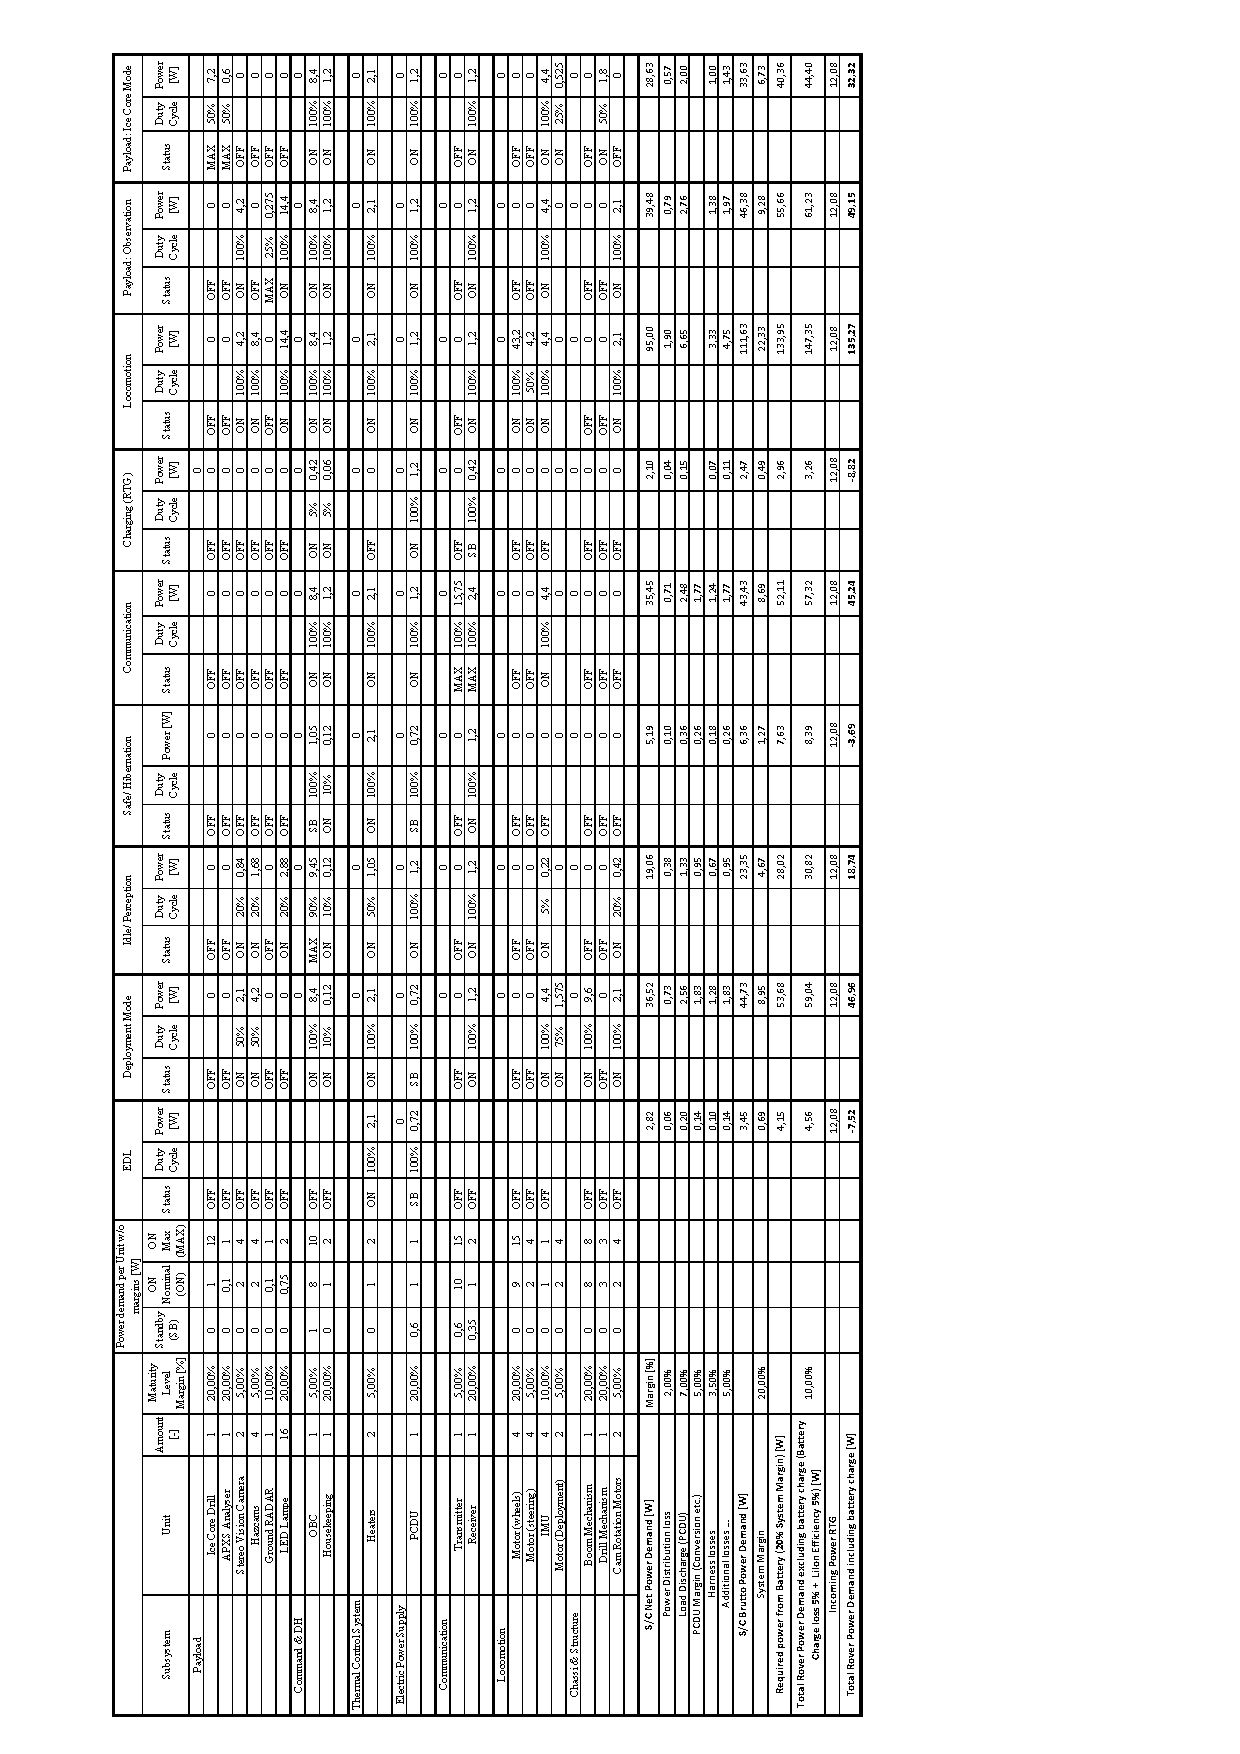
\includegraphics[width=1.0\textwidth]{Media/budgeteps}
\caption{Holistic Power Budget of INPSIRE.}
\label{tab:powerbudgetcomplete}
}
\end{figure}

\clearpage

\setcounter{figure}{0}
\setcounter{table}{0}

%-------------------------------------------------
\section{Communications} 
\label{sec:AppendixCOM}
%-------------------------------------------------

\subsection{Link Budget}
\label{app:LinkBudget}

Link budget considerations are performed under the conservative assumptions listed in \autoref{tab:lb-param}. \\

\begin{table}[h]
\centering
\begin{tabular}{llclll}
\hline
Parameter                        & Value  & Unit	       & Symbol        & Source                       &  \\ \hline
Rover                            &        &            &               &                              &  \\ \hline\hline
antenna Gain           		     & 2      & {[}dB{]}   & ${G}_{R}$  	   & omnidirectional LGA          &  \\
output power        	         & 1      & {[}W{]}    & ${P}_{R}$  	   &                              &  \\
line loss               	     & 0,6    & {[}dB{]}   & ${L}_{l1}$ 	   & FLP                          &  \\ \hline
Path                             &        &            &               &                              &  \\ \hline\hline
R2L polarisation loss            & 0,3    & {[}dB{]}   & ${L}_{p}$ 	   & FLP                          &  \\
free space loss                  & 117,55 & {[}$m^3${]}& ${L}_{s}$  	   &                              &  \\
atmospheric loss                 & 0      & {[}dB{]}   & ${L}_{a}$	   & negligible atmosphere        &  \\ \hline
Lander                           &        &            &               &                              &  \\ \hline\hline
antenna Gain             		 & 1      & {[}dB{]}   & ${G}_{L}$	   & conservative estimation      &  \\
output power        	         & 5      & {[}W{]}    & ${P}_{L}$  	   & conservative estimation      &  \\
pointing Loss  		             & 0      & {[}dB{]}   & ${n/a}$       & omnidirectional LGA          &  \\
line Loss  		                 & 0,6    & {[}dB{]}   & ${L}_{l2}$	   & FLP                          &  \\
eff. noise temperature           & 300    & {[}K{]}    & ${T}_{s}$	   & worst case E-bay temperature &  \\ \hline
Demodulation \& Uncertain Losses &        &            &               &                              &  \\ \hline\hline
eff. data rate                   & 5000   & {[}kbps{]} & ${R}$         & 50 \% of max. data rate                            &  \\
FEC coding                       & none   & {[}-{]}    & ${n/a}$       &                              &  \\
technical degradation            & 1      & {[}dB{]}   & ${L}_{i1}$    & FLP                          &  \\
implementation loss              & 1      & {[}dB{]}   & ${L}_{i1}$	   & FLP                          &  \\
                                 &        &            &               &                              & 
\end{tabular}
\caption{Transmission link parameters}
\label{tab:lb-param}
\end{table}

The free space loss ${L}_{s}$ [$m^3$] in \autoref{tab:lb-param} is calculated using the following correlation. 

\begin{equation}
	\centering
		{L}_{s} = {\frac{(4 \pi s)^2 \cdot c}{f}}
	\label{eqn:Ls}
\end{equation}

The signal travel distance {s} is assumed to be $s = 2000\ m$ which is in excess of the mission goal described in \autoref{chap:sc-output}. In accordance with X-Band communication the frequency {f} is set to a value of $f = 8,2\ GHz$. The parameter c represents the speed of light in vacuum. For simplification purposes $c = 3 \cdot 10^9\ \frac{m}{s}$ is assumed. \\ \\   
Combining the parameters from \autoref{tab:lb-param} the link budget is calculated using \autoref{eqn:EbzuN0}. For the simplification of \autoref{eqn:EbzuN0} the line losses for the rover ${L}_{l1}$ and lander ${L}_{l2}$ are expressed as the sum ${L}_{l}$. In the same manner technical degradation and implementation losses are combined to ${L}_{i}$. Atmospheric losses ${L}_{a}$ and pointing errors in \autoref{eqn:EbzuN0} are neglected due to a lack of atmosphere and the utilisation of omnidirectional low gain antennas. Parameter ${k}$ describes the Boltzmann constant.   

\begin{equation}
  \centering
		{\frac{{E}_{b}}{{N}_{0}}} = {P} - {L}_{l} + {G}_{R} - {10\cdot \log{{L}_{s}}} - {L}_{a} + {G}_{L} + {10\cdot \log{k}} - {10\cdot \log{{T}_{s}}} - {10\cdot \log{{R}}} - {L}_{i}
	\label{eqn:EbzuN0}
\end{equation}


\autoref{eqn:EbzuN0} and the conservative assumptions from \autoref{tab:lb-param} results in an energy per bit over noise $\frac{{E}_{b}}{{N}_{0}} = 10,59\ dB$. The complete link budget can be found in \autoref{fig:LB-R2L}. \\
Referencing \autoref{fig:BitErrorRate} a Bit Error Rate of $10^{-4}$ can be achieved in the downlink path, which is considered sufficient for a first assessment. Optionally a FEC code can be implemented in later design phases.\\

Using the same parameters listed in \autoref{tab:lb-param} leads to a $\frac{{E}_{b}}{{N}_{0}} = 50,56\ dB$ corresponding to a Bit Error Rate of potentially less than $10^{-6}$. Therefore the downlink does not contribute to the design decisions. The complete link budget for the uplink path can be found in \autoref{fig:LB-L2R}.

%Complete Link Budget for Rover to Lander Transmission
\begin{table}[]
\centering
\caption{Complete link budget for Rover to Lander transmission.}
\label{tab:lb-R2L}
\begin{tabular}{llll}
\multicolumn{4}{l}{Rover to Lander (R2L) Link Budget (uplink)}                   \\ \hline
\multicolumn{4}{l}{\cellcolor[HTML]{DAE8FC}Rover}                                \\
Rover transmitter output power            &${P}_{R}$		& 1                      & W    \\
                                          &${P}_{R}$    & 0                      & dB   \\
Rover line loss                           &${L}_{l1}$   & 0.6                    & dB   \\
Rover antenna gain                        &${G}_{R}$ 	& 2                      & dB   \\
\multicolumn{4}{l}{\cellcolor[HTML]{DAE8FC}Downlink Path}                        \\
Rover antenna pointing loss               &n/a    		& 0                      & dB   \\
polarization loss                     	  &${L}_{p}$		& 0.3                    & dB   \\
free space loss                           &${L}_{s}$		& 116.74                 & dB   \\
atmospheric loss                          &${L}_{a}$		& 0                      & dB   \\ \hline
signal level at Lander                    &RIP      		& -115.64                & dB   \\
\multicolumn{4}{l}{\cellcolor[HTML]{DAE8FC}Lander}                               \\
Lander LGA pointing loss                  &      		& 0                      & dB   \\
Lander antenna gain                       &${G}_{L}$		& 1                      & dB   \\ \hline
signal after Lander LGA                   &      		& -114.64                & dB   \\ \hline
Lander line loss                    		  &${L}_{l2}$	& 0.6                    & dB   \\
Lander effective noise temp.              &${T}_{s}$ 	& 24.77                  & dB   \\ \hline
Lander signal to noise power density      & $\frac{C}{{N}_{0}}$ & 88.58                  & dB   \\ \hline
\multicolumn{4}{l}{\cellcolor[HTML]{DAE8FC}Data Rate}                            \\ \hline
data rate                                 &${R}$			& 5000                   & kbps \\
                                          &${R}$			& -66.99                 & dBHz \\ \hline
\multicolumn{4}{l}{\cellcolor[HTML]{DAE8FC}Total}                                \\ \hline
System $\frac{{E}_{b}}{{N}_{0}}$ for L2R link &$\frac{{E}_{b}}{{N}_{0}}$& 21.59                  & dB   \\
\multicolumn{4}{l}{}                                                             \\ \hline
\multicolumn{4}{l}{\cellcolor[HTML]{DAE8FC}Demodulation}                         \\ \hline
specified Bit Error Rate                  &BER      		& $10^{-4}$ 				 & n/a  \\
FEC coding used                           &      		& none                   &      \\
$\frac{{E}_{b}}{{N}_{0}}$ threshold       &      		& 9                      & dB   \\ \hline
\multicolumn{4}{l}{\cellcolor[HTML]{DAE8FC}Uncertain Losses}                     \\ \hline
technical degradation                     &${L}_{i1}$	& 1                      & dB   \\
implementation loss                       &${L}_{i2}$	& 1                      & dB   \\
\multicolumn{4}{l}{}                                                             \\ \hline
\multicolumn{4}{l}{\cellcolor[HTML]{DAE8FC}Link Margin}                          \\ \hline
system link margin after uncertain losses &$\frac{{E}_{b}}{{N}_{0}}$& 10.59                  & dB  
\end{tabular}
\end{table}

%Complete Link Budget for Lander to Rover Transmission
\begin{table}[]
\centering
\caption{Complete link budget for Lander to Rover (L2R) transmission.}
\label{tab:lb-L2R}
\begin{tabular}{llll}
\multicolumn{4}{l}{Lander to Rover (L2R) Link Budget (downlink)}                 \\ \hline
\multicolumn{4}{l}{\cellcolor[HTML]{DAE8FC}Lander}                               \\
Lander transmitter output power           &${P}_{L}$		& 5                      & W    \\
                                          &${P}_{L}$		& 6.99                   & dB   \\
Lander line loss                          &${L}_{l2}$	& 0.6                    & dB   \\
Lander antenna gain                       &${G}_{L}$		& 1                      & dB   \\
\multicolumn{4}{l}{\cellcolor[HTML]{DAE8FC}Uplink Path}                          \\
pointing loss                             &n/a	    		& 0                      & dB   \\
polarization loss                         &${L}_{p}$		& 0.3                    & dB   \\
free space loss                           &${L}_{s}$		& 116.74                 & dB   \\
atmospheric loss                          &${L}_{a}$		& 0                      & dB   \\ \hline
signal level at Lander					  & RIP  & 109.65				  & dB   \\ 
\multicolumn{4}{l}{\cellcolor[HTML]{DAE8FC}Rover}                                \\
Rover LGA pointing loss                   &n/a	    		& 0                      & dB   \\
Rover antenna gain                        &${G}_{R}$		& 1                      & dB   \\ \hline
signal after Rover LGA                    &      		& 108.65                 & dB   \\ \hline
Rover line loss                     	      &${L}_{l1}$	& 0.6                    & dB   \\
Rover effective noise temp.               &${T}_{s}$ 	& 24.77                  & dB   \\ \hline
Rover signal to noise power density       & $\frac{C}{{N}_{0}}$	 & 94.57                  & dB   \\ \hline
\multicolumn{4}{l}{\cellcolor[HTML]{DAE8FC}Data Rate}                            \\ \hline
data rate                                 &${R}$   		& 2                      & kbps \\
                                          &${R}$ 		& 33.01                  & dBHz \\ \hline
\multicolumn{4}{l}{\cellcolor[HTML]{DAE8FC}Total}                                \\ \hline
System $\frac{{E}_{b}}{{N}_{0}}$for L2R link &      		& 61.56                  & dB   \\
\multicolumn{4}{l}{}                                                             \\ \hline
\multicolumn{4}{l}{\cellcolor[HTML]{DAE8FC}Demodulation}                         \\ \hline
specified Bit Error Rate                  &BER      		& $10^{-6}$ 			  & n/a  \\
FEC coding used                           &      		& none                   &      \\
$\frac{{E}_{b}}{{N}_{0}}$ threshold       &				& 11                     & dB   \\ \hline
\multicolumn{4}{l}{\cellcolor[HTML]{DAE8FC}Uncertain Losses}                     \\ \hline
technical degradation                     &${L}_{i1}$	& 1                      & dB   \\
implementation loss                       &${L}_{i1}$	& 1                      & dB   \\
\multicolumn{4}{l}{}                                                             \\ \hline
\multicolumn{4}{l}{\cellcolor[HTML]{DAE8FC}Link Margin}                          \\ \hline
system link margin after uncertain losses &$\frac{{E}_{b}}{{N}_{0}}$	& 48.56      & dB  
\end{tabular}
\end{table}

\begin{figure}[h]
	\centering
  		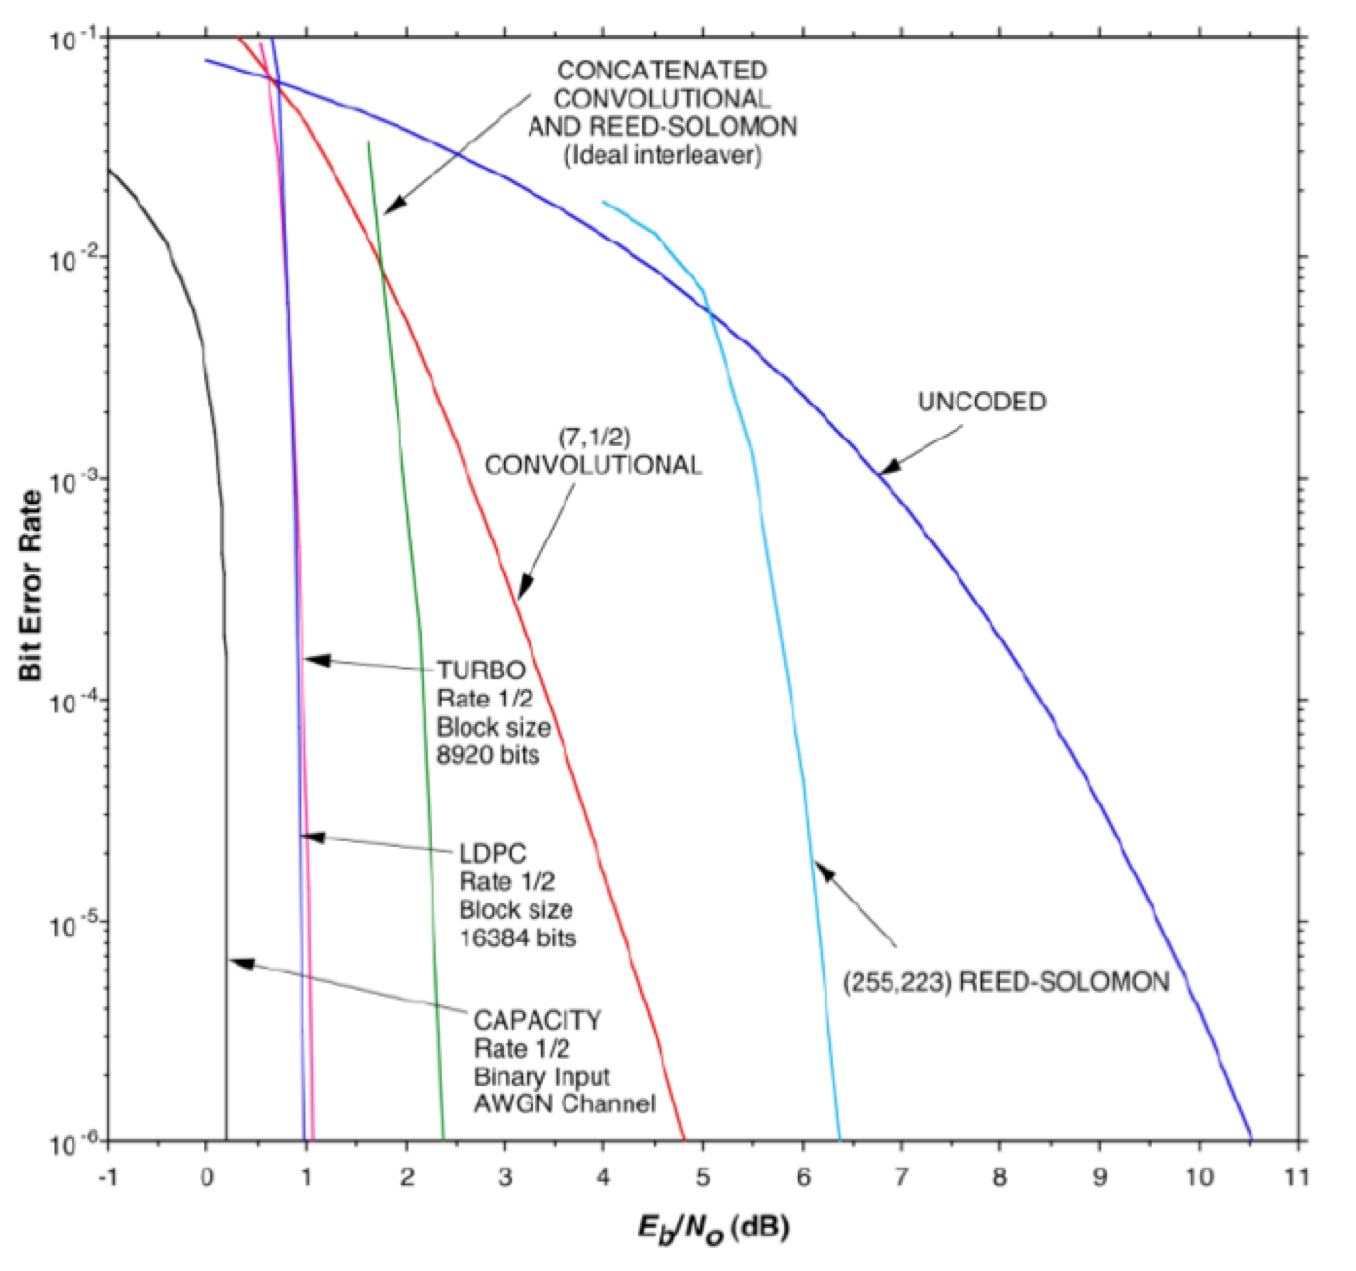
\includegraphics[width=0.9\textwidth]{Media/Bit_Error_Rate.png}
  \caption{Bit Error Rate for different FEC codes}
  \label{fig:BitErrorRate}
\end{figure}

\subsection{Mission Data Output}
\label{app:MissionDataOutput}

The analysis of the mission data concept for memory capacity and transmission times is focuses on the payload camera and Hazcams as images require far more data than telemetry or other payload data. \\

In a first assumption 420 images per day are stored and transmitted. Considering the sensor resolution of $2048\times2048$ pixels and a bit depth per pixel of 10 bit of the (CAMERA REFERENCE), a file size of 42 Mbit per image is assumed.\\
To calculate the message size in \autoref{tab:TimePerPic}, it is assumed that a transmission frame consists of 10264 bits including a payload frame of maximum 8840 bits (FLP VORELESUNG).   

\begin{table}[h]
\centering
\begin{tabular}{llllll}
File Type & Compression    & File Size  & Message Size & Data Rate & Tx t per File \\ \hline\hline
image     & none           & 42 Mbit    & 48,77 Mbit   & 5 Mbit    & 8,12 s        \\
image     & HIREW          & 23,52 Mbit & 27,31 Mbit   & 5 Mbit    & 5,45 s        \\ \hline
\end{tabular}
\caption{Comparison of transmission times per image (message frame bits included)}
\label{tab:TimePerPic}
\end{table}

\begin{table}[h]
\centering
\begin{tabular}{lllll}
File per tal & Compression & File Size  & Total Data & Tx time    \\ \hline\hline
420          & none        & 42 Mbit    & 2,21 GB    & 56,9 Min.  \\
420          & HIREW       & 23,52 Mbit & 1,22 GB    & 38,23 Min. \\ \hline
\end{tabular}
\caption{Transmission time and total data output per mission day}
\label{tab:Tx-tptal}
\end{table}

The HIREW compression algorithm is suggested for the mission considering a high average compression of 0,56 \% and a high compression speed of 123 Mbit/s for grayscale and 104,4 Mbit/s for RGB image files (COMPRESSSION PAPER REFERENCE). 

\subsection{Communications Trade Off}
\label{app:Com_TrOff}

\subsubsection{Transmitter Selection}
% Transmitter Trade off
\begin{figure}[h]
     \centering
     \begin{subfigure}[b]{0.49\textwidth}
         \centering
         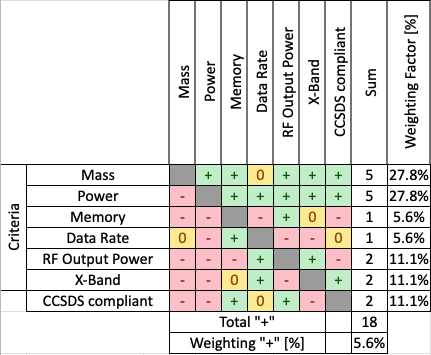
\includegraphics[width=\textwidth]{Media/Trade_off/Transmitter/Weighting_trans.png}
         \caption{Weighting of selection criteria for the transmitter.}
         \label{fig:Weighting_trans}
     \end{subfigure}
     \hfill
     \begin{subfigure}[b]{0.49\textwidth}
         \centering
         \includegraphics[width=\textwidth]{Media/Trade_off/Transmitter/Values_trans.png}
         \caption{Comparison of optional transmitters.}
         \label{fig:Values_trans}
     \end{subfigure}
     \hfill
     \begin{subfigure}[b]{0.49\textwidth}
         \centering
         \includegraphics[width=\textwidth]{Media/Trade_off/Transmitter/TradeOff_trans.png}
         \caption{Transmitter trade off.}
         \label{fig:TradeOff_trans}
     \end{subfigure}
     \hfill
     \caption{Transmitter Trade off for the Communication subsystem.}
     \label{TrOff_Trans}
\end{figure}

\subsubsection{Receiver Trade Off}
%Receiver Trade Off
\begin{figure}[h]
     \centering
     \begin{subfigure}[b]{0.49\textwidth}
         \centering
         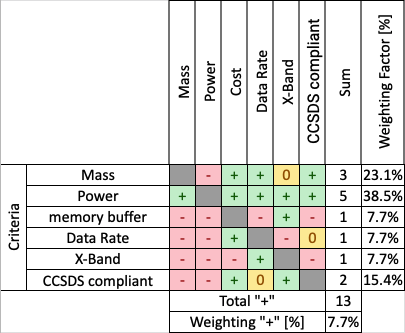
\includegraphics[width=\textwidth]{Media/Trade_off/Receiver/Weighting_Rec.png}
         \caption{Weighting of selection criteria for the receiver.}
         \label{fig:Weighting_Rec}
     \end{subfigure}
     \hfill
     \begin{subfigure}[b]{0.49\textwidth}
         \centering
         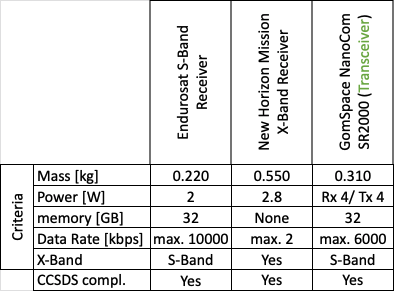
\includegraphics[width=\textwidth]{Media/Trade_off/Receiver/Values_Rec.png}
         \caption{Comparison of optional receivers.}
         \label{fig:Values_Rec}
     \end{subfigure}
     \hfill
     \begin{subfigure}[b]{0.49\textwidth}
         \centering
         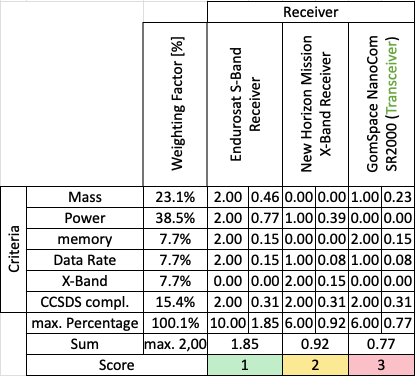
\includegraphics[width=\textwidth]{Media/Trade_off/Receiver/TradeOff_Rec.png}
         \caption{Receiver trade off.}
         \label{fig:TradeOff_Rec}
     \end{subfigure}
     \hfill
     \caption{Receiver Trade off for the Communication subsystem.}
     \label{TrOff_Trans}
\end{figure}

\subsubsection{Antenna Trade Off}
%Antenna Trade Off
\begin{figure}[h]
     \centering
     \begin{subfigure}[b]{0.49\textwidth}
         \centering
         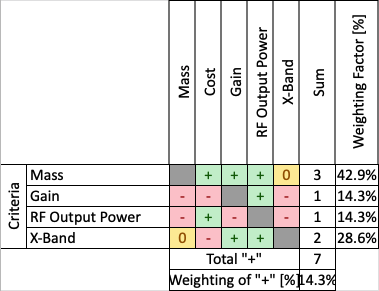
\includegraphics[width=\textwidth]{Media/Trade_off/Antenna/Weighting_Ant.png}
         \caption{Weighting of selection criteria for the antenna.}
         \label{fig:Weighting_Rec}
     \end{subfigure}
     \hfill
     \begin{subfigure}[b]{0.49\textwidth}
         \centering
         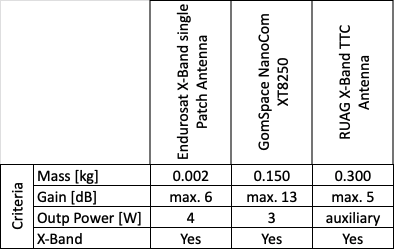
\includegraphics[width=\textwidth]{Media/Trade_off/Antenna/Values_Ant.png}
         \caption{Comparison of optional antenna.}
         \label{fig:Values_Rec}
     \end{subfigure}
     \hfill
     \begin{subfigure}[b]{0.49\textwidth}
         \centering
         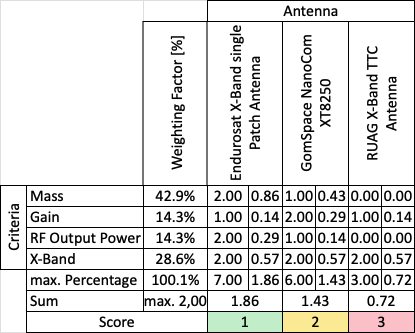
\includegraphics[width=\textwidth]{Media/Trade_off/Antenna/TradeOff_Ant.png}
         \caption{Antenna trade off.}
         \label{fig:TradeOff_Rec}
     \end{subfigure}
     \hfill
     \caption{Antenna trade off for the Communication subsystem.}
     \label{TrOff_Trans}
\end{figure}

\subsection{Command \& Data Handling Trade Off}

\subsubsection{OBC Trade Off}
%OBC Trade Off
\begin{figure}[htb]
     \centering
     \begin{subfigure}[b]{0.49\textwidth}
         \centering
         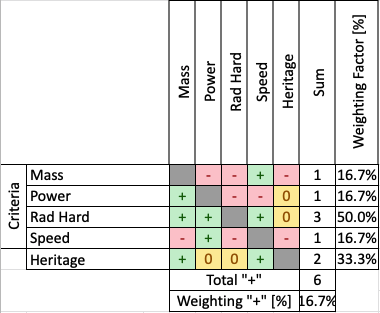
\includegraphics[width=\textwidth]{Media/Trade_off/OBC/Weighting_OBC.png}
         \caption{Weighting of selection criteria for the OBC.}
         \label{fig:Weighting_Rec}
     \end{subfigure}
     \hfill
     \begin{subfigure}[b]{0.49\textwidth}
         \centering
         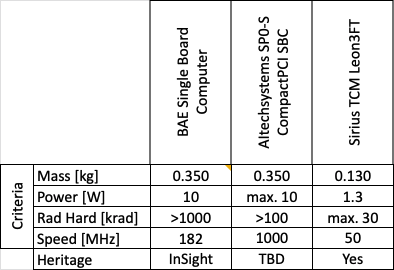
\includegraphics[width=\textwidth]{Media/Trade_off/OBC/Values_OBC.png}
         \caption{Comparison of optional single board computers.}
         \label{fig:Values_Rec}
     \end{subfigure}
     \hfill
     \begin{subfigure}[b]{0.49\textwidth}
         \centering
         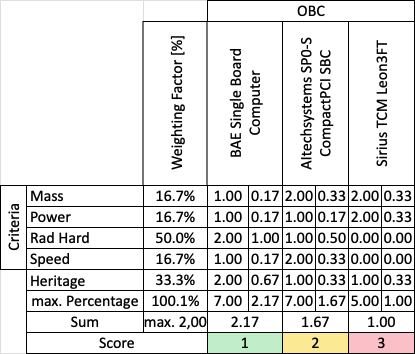
\includegraphics[width=\textwidth]{Media/Trade_off/OBC/TradeOff_OBC.png}
         \caption{Antenna trade off.}
         \label{fig:TradeOff_Rec}
     \end{subfigure}
     \hfill
     \caption{OBC trade off for the Command \& Data Handling subsystem.}
     \label{TrOff_Trans}
\end{figure}

\clearpage

\setcounter{figure}{0}
\setcounter{table}{0}

%-------------------------------------------------
\section{Thermal Controls System} \label{sec:AppendixThermal}
%-------------------------------------------------
\subsection{Results}
\begin{table}[htb]
	\centering
	\caption{Temperature results in K of thermal analysis, \textit{with out}  margin .}
	\begin{tabular}{lccccc}
		\toprule
		Components & Hot Case & Cold Case & Charging & Communication & Analyse  \\ \midrule
		RTG  & 415 & 391 & 402 & 407  &  401   \\
		Electric Bay & 301 & 268 & 293 & 313 & 28 \\
		Drill  & 283 & 256 & 267 & 271 & 328  \\
		Camera & 327 & 249 & 256 & 257 & 256 \\
		Chassis & 268 & 230  & 245 & 251 & 246 \\
		Steer Engine & 296 & 249 & 260 & 262 & 261  \\
		Drive Engine & 344 & 251 & 262 & 262 & 262 \\   \bottomrule
	\end{tabular}
	\label{tab:tcs_temp1}
\end{table}

\begin{table}[htb]
	\centering
	\caption{Temperature results in K of thermal analysis, \textit{with}  margin .}
	\begin{tabular}{lccccc}
		\hline
		Components & Hot Case & Cold Case & Charging & Communication & Analyse  \\[0.25em]
		Margin & +15~K & -15~K & +15~K & +15~K & +15~K \\ \hline
		RTG  & 430 & 376 & 417 & 422  & 416    \\
		Electric Bay & 316 & 253 & 308 & 328 & 296 \\
		Drill  & 298 & 241 & 282 & 286 & 343  \\
		Camera & 342 & 234 & 271 & 272 & 271 \\
		Chassis & 283 & 215 & 260 & 266 & 261 \\
		Steering Engine & 311 & 234 & 275 & 277 & 276  \\
		Drive Engine & 359 & 236 & 277 & 277 & 277 \\   \hline
	\end{tabular}
	\label{tab:tcs_temp2}
\end{table}



\subsection{Heat energy eqilibrium}  \label{sec:app_tcs_01}
The follwing equiations describe each node of the thermal network.
The input values were tanken from EPS, \autoref{sec:app_therm_2}, \autoref{sec:app_therm_3}, \autoref{sec:app_therm_4} respectively.

\begin{table}[H]
	\begin{tabular}{l@{\quad}l@{\qquad\qquad\qquad}l@{\quad}l}
		\multicolumn{4}{l}{\textit{Subscript} for eqilibrium:}\\[0.5em]
		Bay & Electrical Bay & D	& Drill\\
		Bo & Bogie & 	E,D & Drive Engine\\
		Cam & Camera & E,S & Steer Engine\\
		C & Chassis & WF & Wheel Fork\\
	\end{tabular}

\end{table}

\underline{RTG:}
\begin{equation}
\begin{aligned}
0=\  &\dot{Q}_{RTG} +CON_1 \cdot (T_{Bay}-T_{RTG})+CON_2 \cdot (T_{C}-T_{RTG})+ \\[1em]
& + CON_5 \cdot (T_{D}-T_{RTG})+ CON_9 \cdot (T_{E,S}-T_{RTG})\\[1em]
& +   CON_12 \cdot (T_{E,D}-T_{RTG}) - \epsilon_{RTG}\cdot \sigma_b \cdot S_{RTG}\cdot T_{RTG}^4 \\[2em]
\end{aligned}
\end{equation}

\underline{Electric Bay:}
\begin{equation}
	\begin{aligned}
		0=\ &  \dot{Q}_{Bay}+ CON_1 \cdot (T_{RTG}-T_{Bay})+ (CON_3+n_{S2}\cdot CON_{S2}) \cdot (T_{C}-T_{Bay})-\\[1em]
		&  -\epsilon_{Bay}\cdot \sigma_b \cdot S_{Bay}\cdot T_{Bay}^4
	\end{aligned}
\end{equation}\\
with: 
\begin{equation} \dot{Q}_{Bay} = \dot{Q}_{OBC} + \dot{Q}_{Tranceiver} +\dot{Q}_{Receiver} +\dot{Q}_{PCDU} \end{equation}\\

\underline{Drill \& Analyser:}
\begin{equation} 0= \ \dot{Q}_{D} +CON_4 \cdot (T_{C}-T_{D})+CON_5 \cdot (T_{RTG}-T_{D})   \end{equation} \\
%
\underline{Camera:}
\begin{equation}
\begin{aligned}
0=\  &  \dot{Q}_{Cam} + \dot{Q}_{RHU} +CON_6 \cdot (T_{C}-T_{Cam})+ \\[1em]
& +(CON_{14} +n_{S1}\cdot CON_{S1}) \cdot (T_{Rad}-T_{Cam})  -\\[1em]
& - \epsilon_{Cam}\cdot \sigma_b \cdot S_{Cam}\cdot T_{Cam}^4 \\[2em]
\end{aligned}
\end{equation}
%
\underline{Radiator:}
\begin{equation}0=(CON_{14} +n_{S1}\cdot CON_{S1}) \cdot (T_{Cam}-T_{Rad}) - \epsilon_{Rad}\cdot \sigma_b \cdot S_{Rad}\cdot T_{Rad}^4  \end{equation}  \\
%
\underline{Chassis:}
\begin{equation}
\begin{aligned}
0=\  &   \dot{Q}_{Radar}+\dot{Q}_{Hazcam} +\dot{Q}_{Analyser} +\dot{Q}_{IMUs} +\\[1em]
	& +CON_2 \cdot (T_{RTG}-T_{C})+(CON_3+n_{S2}\cdot CON_{S2})\cdot (T_{Bay}-T_{C})+ \\[1em]
&  +  CON_4 \cdot (T_{Drill}-T_{C})+CON_6 \cdot (T_{Cam}-T_{C})+CON_7 \cdot (T_{Node_1}-T_{C}) +  \\[1em]
&  + \alpha_{C}\cdot [ S_0 \cdot (1+\rho_E) \cdot (S_{Ch1} \cdot \varphi_1  +S_{Ch2} \cdot \varphi_2 ) +   \epsilon_{E} \cdot \sigma_b \cdot S_{Ch3}\cdot T_{Surface}^4 ]+  \\[1em]
& +\epsilon_{Bay}\cdot \sigma_b \cdot S_{Bay}\cdot T_{Bay}^4 - \frac{1}{2} \cdot \epsilon_{Bo}\cdot \sigma_b \cdot S_{Bo}\cdot \left( \frac{T_{C}}{2} +\frac{T_{Node_1}}{2}  \right)^4  -\epsilon_{C}\cdot \sigma_b \cdot S_{C}\cdot T_{C}^4 \\[2em]
\end{aligned}
\end{equation}

\underline{Steer Engine:}
\begin{equation}
\begin{aligned}
0=\  &  4\cdot [\dot{Q}_{E,S} +CON_8  \cdot (T_{Node1}-T_{E,S})+ \\[1em]
&   +CON_9 \cdot (T_{RTG}-T_{E,S}) -\epsilon_{E,S}\cdot \sigma_b \cdot S_{E,S}\cdot T_{E,S}^4] \\[2em]
\end{aligned}
\end{equation}

\underline{Distribution Node 1:}
\begin{equation}
\begin{aligned}
0=\  &  4\cdot [CON_7 \cdot (T_{C}-T_{Node_1})+CON_8 \cdot (T_{E,S}-T_{Node_1})+ \\[1em]
&   +CON_10 \cdot (T_{Node_2}-T_{Node_1}) - \\[1em]
&  - \frac{1}{2} \cdot \epsilon_{Bo}\cdot \sigma_b \cdot S_{Bo}\cdot \left( \frac{T_{C}}{2} +\frac{T_{Node_1}}{2}  \right)^4  - \\[1em]
& - \frac{1}{2} \cdot \epsilon_{WF}\cdot \sigma_b \cdot S_{WF}\cdot \left( \frac{T_{Node_1}}{2} +\frac{T_{Node_2}}{2}  \right)^4- \\[1em]
& -\epsilon_{E,S}\cdot \sigma_b \cdot S_{E,S}\cdot T_{E,S}^4\ ] \\[2em]
\end{aligned}
\end{equation}

\underline{Drive Engine:}
\begin{equation}
\begin{aligned}
0=\  &  4 \cdot [\dot{Q}_{E,D}+ (CON_{11}+n_{S3}\cdot CON_{S3}) \cdot (T_{Node_2}-T_{E,D})+ \\[1em]
&  + CON_{12} \cdot (T_{RTG}-T_{E,D})-\epsilon_{E,D}\cdot \sigma_b \cdot S_{E,D}\cdot T_{E,D}^4 ]  \\[2em]
\end{aligned}
\end{equation}

\underline{Distribution Node 2:}
\begin{equation}
\begin{aligned}
0=\ & 4 \cdot [CON_{10} \cdot (T_{Node_1}-T_{Node_2})+CON_{13} \cdot (T_{Ground}-T_{Node_2}) +   \\[1em]
&   +(CON_{11}+n_{S3}\cdot CON_{S3}) \cdot (T_{E,D}-T_{Node_2}) + \\[1em]
& - \frac{1}{2} \cdot \epsilon_{WF}\cdot \sigma_b \cdot S_{WF}\cdot \left( \frac{T_{Node_1}}{2} +\frac{T_{Node_2}}{2}  \right)^4- \\[1em]
& -\epsilon_{E,D}\cdot \sigma_b \cdot S_{E,D}\cdot T_{E,D}^4\ ] \\[2em]
\end{aligned}
\end{equation}
\clearpage

\subsection{Heat conductance} \label{sec:app_therm_2}

\begin{table}[htb]
	\centering
	\caption{Definition of heat conductance C between the nodes according to \autoref{fig:tcs_network}.}
	\begin{tabular}{l@{\qquad}cccc}
		\hline
		Name &  Linked Components &  \multicolumn{3}{c}{Geometry}\\ \hline
		& & & & \\[-0.75em]
		\textbf{Linkage} & \textbf{RTG} $\leftrightarrow$ \textbf{Chassis}  &  \multicolumn{3}{c}{\multirow{2}{*}{\adjustbox{valign=t}{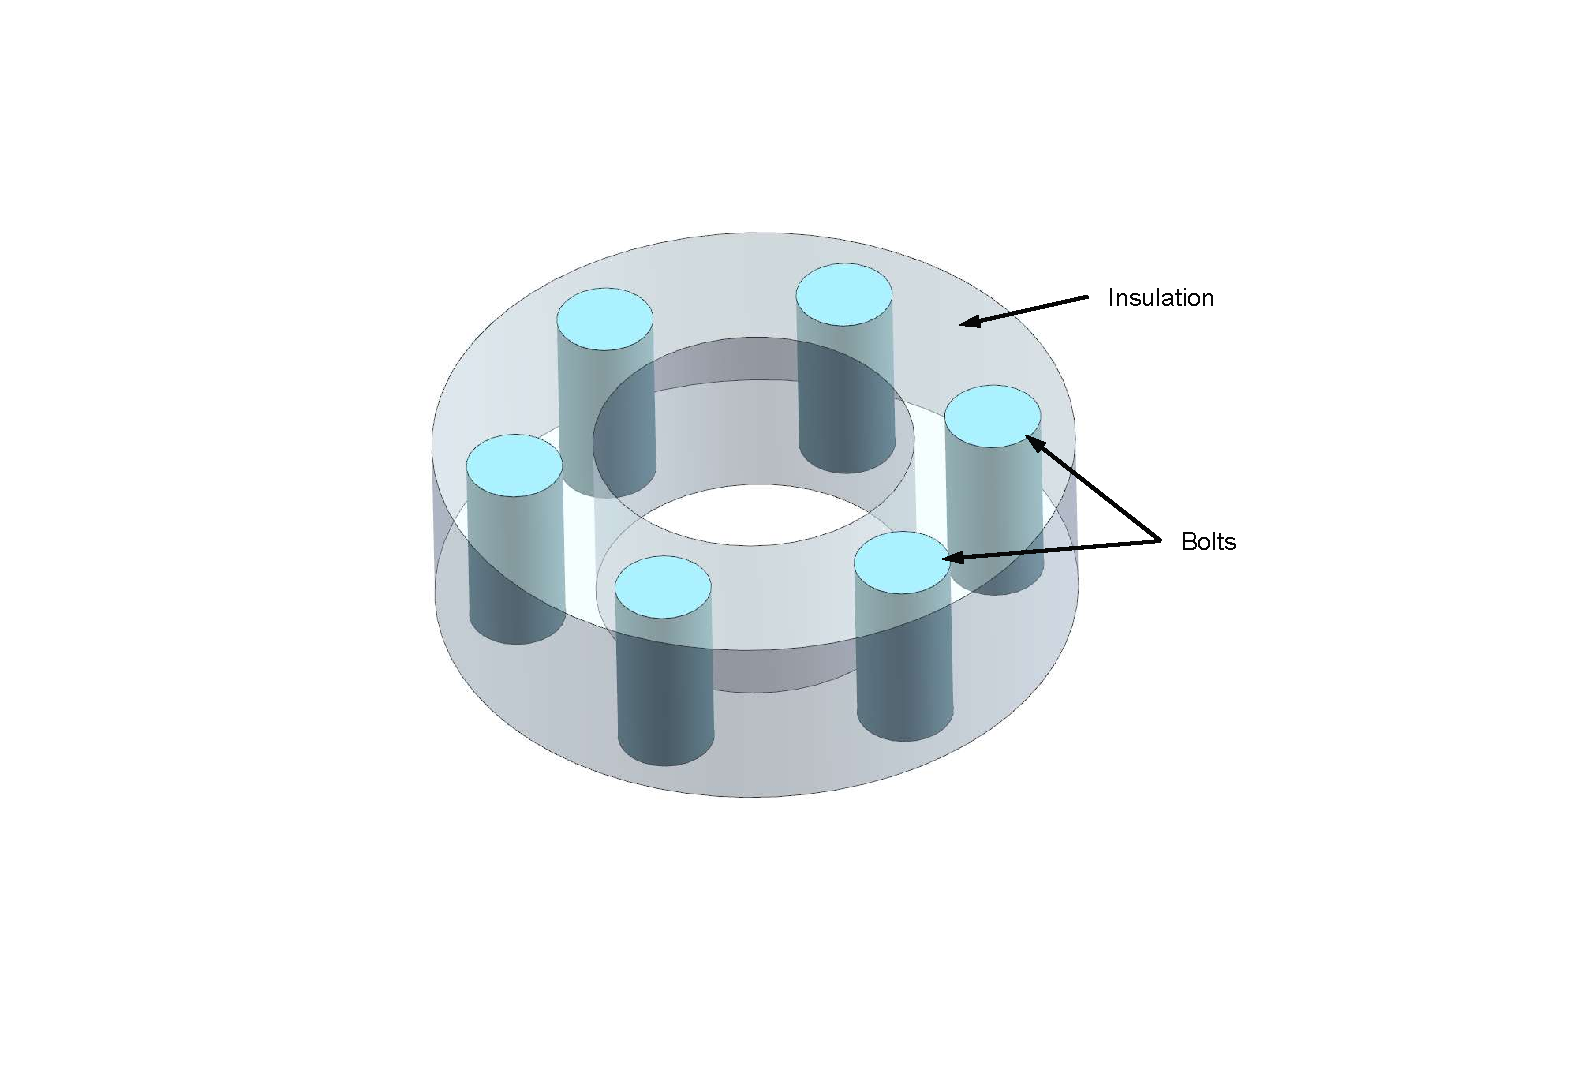
\includegraphics[width=0.3\textwidth]{Media/tcs_con_rtg}}}}  \\[1em]
		& & & &  \\
		\multicolumn{2}{l}{$CON_2= CON_{I}+n_{B}\cdot CON_{B}$} & & & \\[1em]
		\multicolumn{2}{l}{$CON_2= 1.50 \cdot 10^{-1}\ \frac{\W}{\K} $} & & &  \\[3em]
		\hline
		Part &  Cross section & Thickness  & Material & Amount \\ \hline
		& & & & \\[-0.75em]
		Insulation & $S_I=3'770\ \mm^2$ & $t_I=12\ \mm$ & Aerogel & 1 \\[0.5em]
		Bolts, M6 & $S_B=28.3\ \mm^2$ & $t_B=12\ \mm$ & Titan & 10 \\[5em]
		
		\hline
		Name &  Linked Components &  \multicolumn{3}{c}{Geometry}\\ \hline
		& & & & \\[-0.5em]
		\textbf{Linkage} & \textbf{EBay} $\leftrightarrow$ \textbf{Chassis}  &  \multicolumn{3}{c}{\multirow{2}{*}{\adjustbox{valign=t}{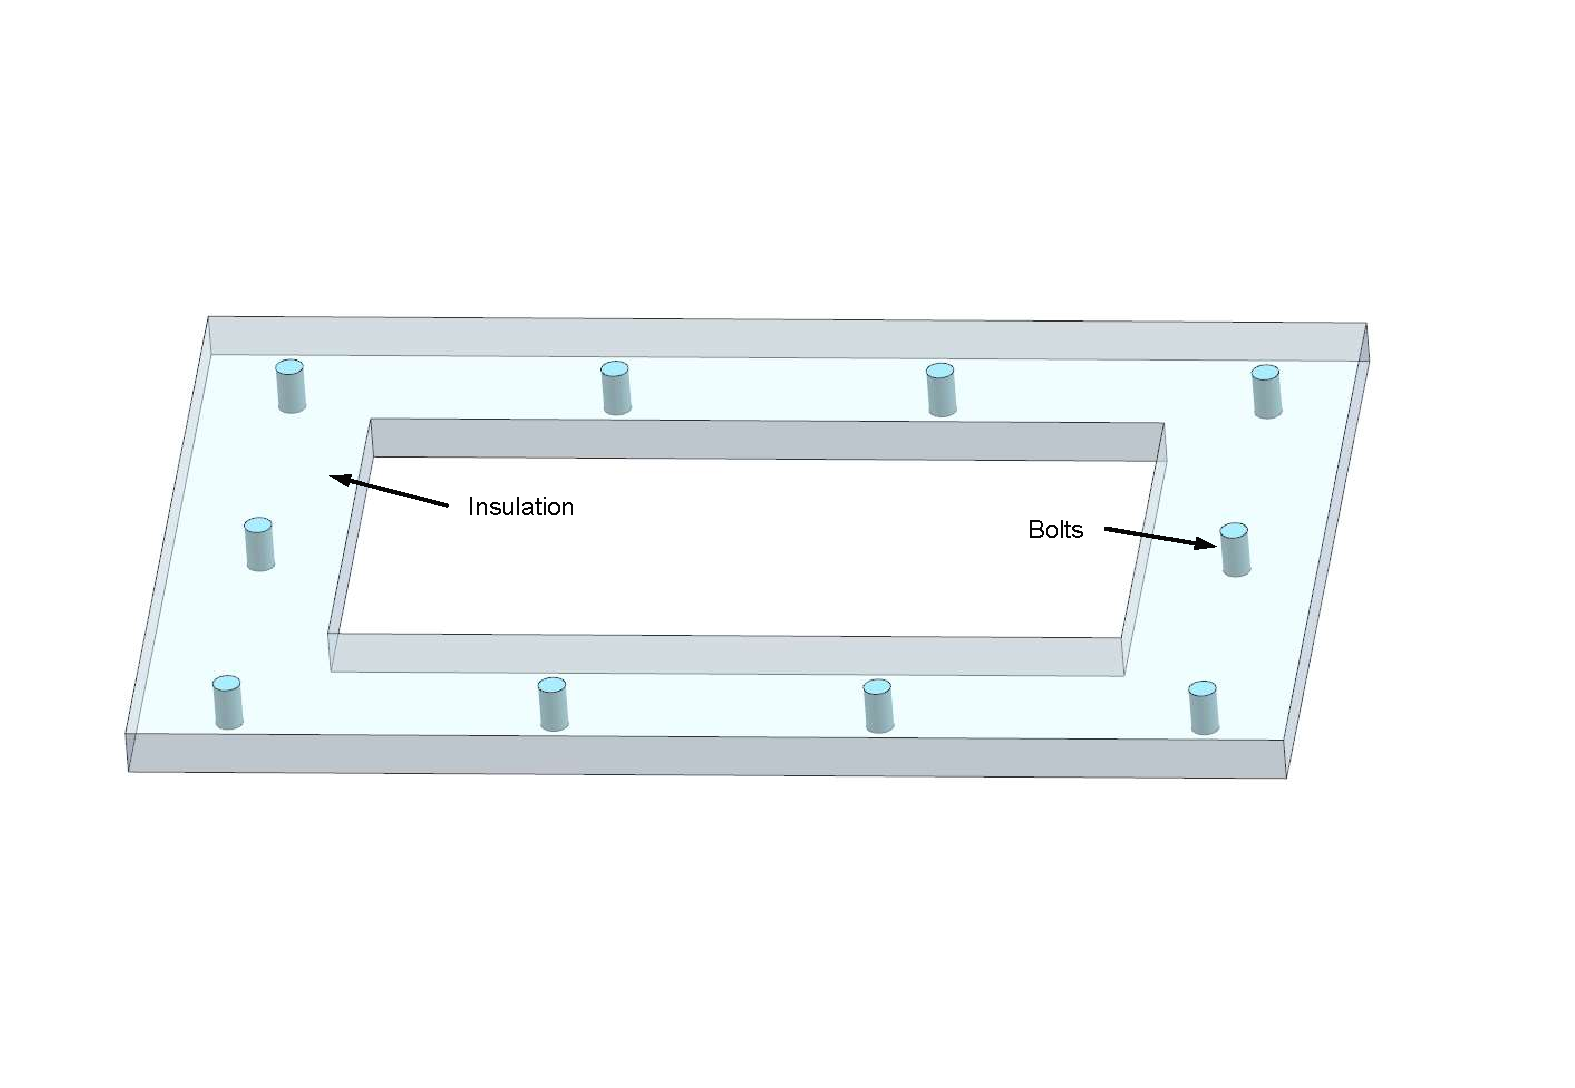
\includegraphics[width=0.5\textwidth]{Media/tcs_con_bay}}}}  \\[1em]
		& & & &  \\
		\multicolumn{2}{l}{$CON_3= CON_{I}+n_{B}\cdot CON_{B}$} & & &  \\[1em]
		\multicolumn{2}{l}{$CON_3= 2.80 \cdot 10^{-1}\ \frac{\W}{\K}$} & & & \\[3em]
		
		\hline
		Part &  Cross section & Thickness  & Material & Amount \\ \hline
		& & & & \\[-0.75em]
		Insulation & $S_I=27'120 \ \mm^2$ & $t_I=12\ \mm$ & Aerogel & 1 \\[0.5em]
		Bolts, M6 & $S_B=28.3 \ \mm^2$ & $t_B=12\ \mm$ & Titan & 10 \\	
	\end{tabular}
	\label{tab:tcs_nodes1}
\end{table}	

\begin{table}[htb]
	\centering
	\caption{Definition of heat conductance $CON=\frac{1}{R}$ between the nodes according to \autoref{fig:tcs_network}.}
	\begin{tabular}{l@{\qquad}cccc}
				\hline
		Name &  Linked Components &  \multicolumn{3}{c}{Geometry}\\ \hline
		& & & & \\[-0.5em]
		\textbf{Linkage} & \textbf{Drill} $\leftrightarrow$ \textbf{Chassis}  &  \multicolumn{3}{c}{\multirow{2}{*}{\adjustbox{valign=t}{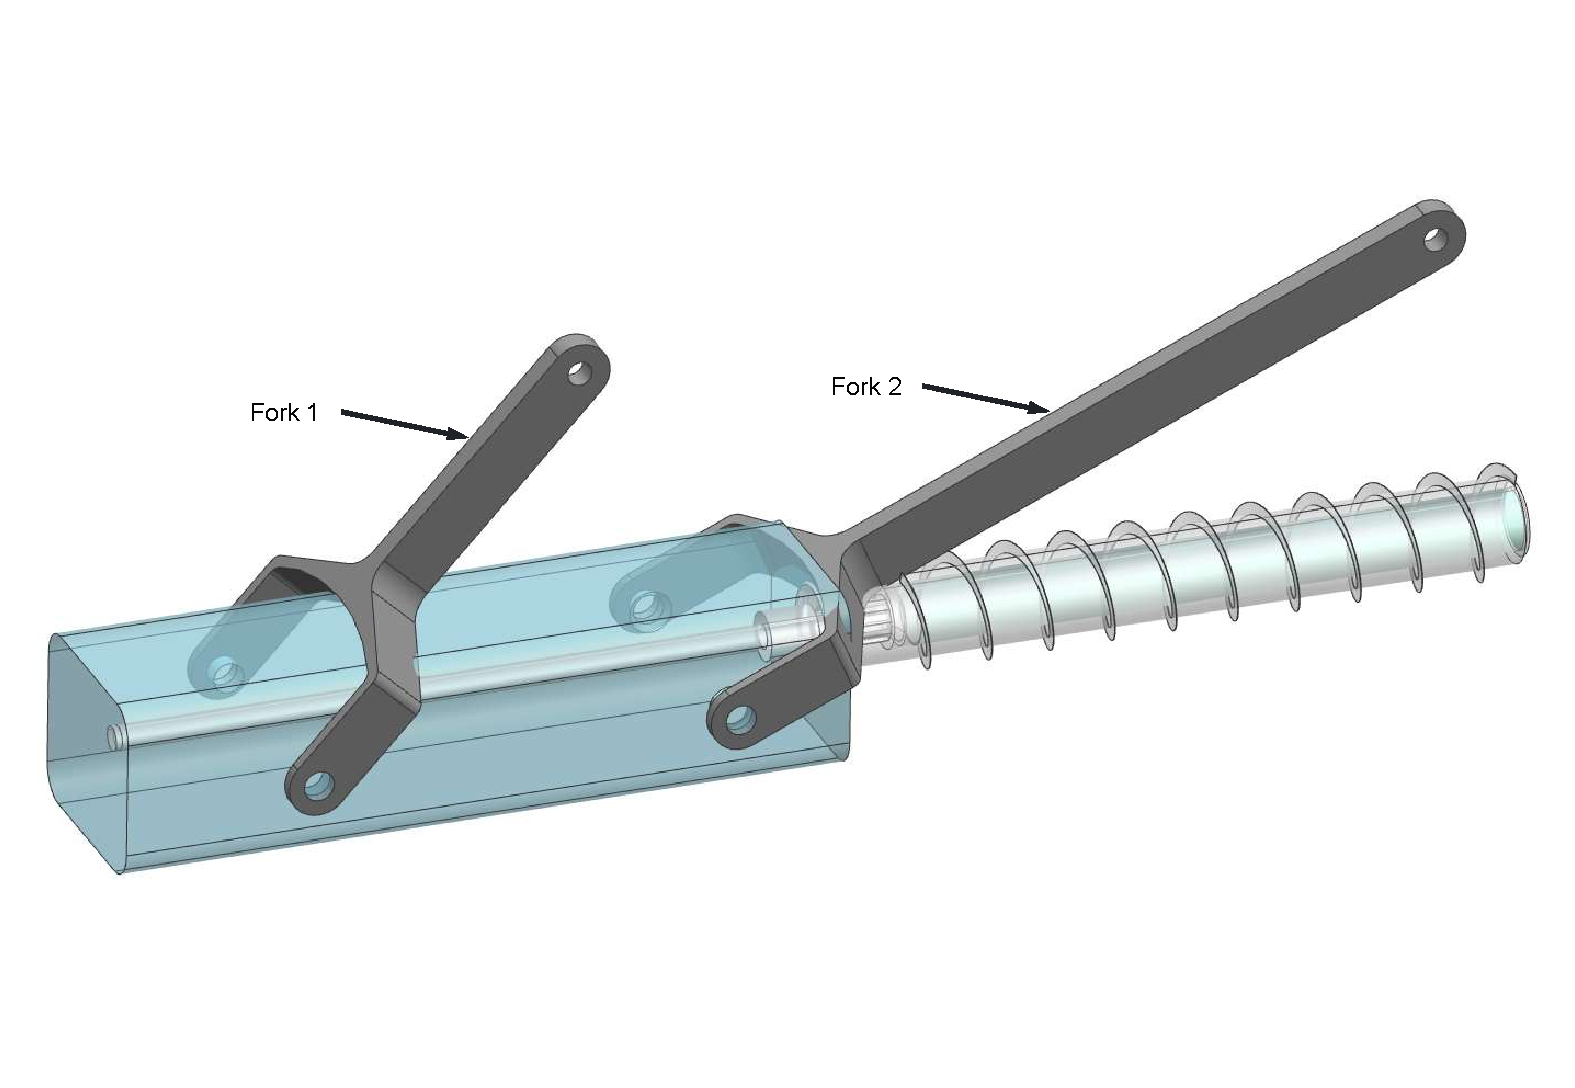
\includegraphics[width=0.55\textwidth]{Media/tcs_con_drill}}}}  \\[1em]
		& & & &  \\
		\multicolumn{2}{l}{$CON_{4}=CON_{F1}+CON_{F2} $} & & & \\[1em]
		\multicolumn{2}{l}{$CON_{4}= 1.56 \cdot 10^{-1}\ \frac{\W}{\K}$} & & & \\[4em]
		
		\hline
		Part &  Cross section & Length  & Material & Amount \\ \hline
		& & & & \\[-0.75em]
		Fork 1& $S_{F1}=40 \ \mm^2$ & $l_{F1}=90$ & Aluminium & 1 \\[0.5em]	
		Fork 1& $S_{F2}=40 \ \mm^2$ & $l_{F2}=150$ & Aluminium & 1 \\[5em]	
		
		
		\hline
		Name &  Linked Components &  \multicolumn{3}{c}{Geometry}\\ \hline
		& & & & \\[-0.5em]
		\textbf{Telescope} & \textbf{Camera} $\leftrightarrow$ \textbf{Chassis}  &  \multicolumn{3}{c}{\multirow{2}{*}{\adjustbox{valign=t}{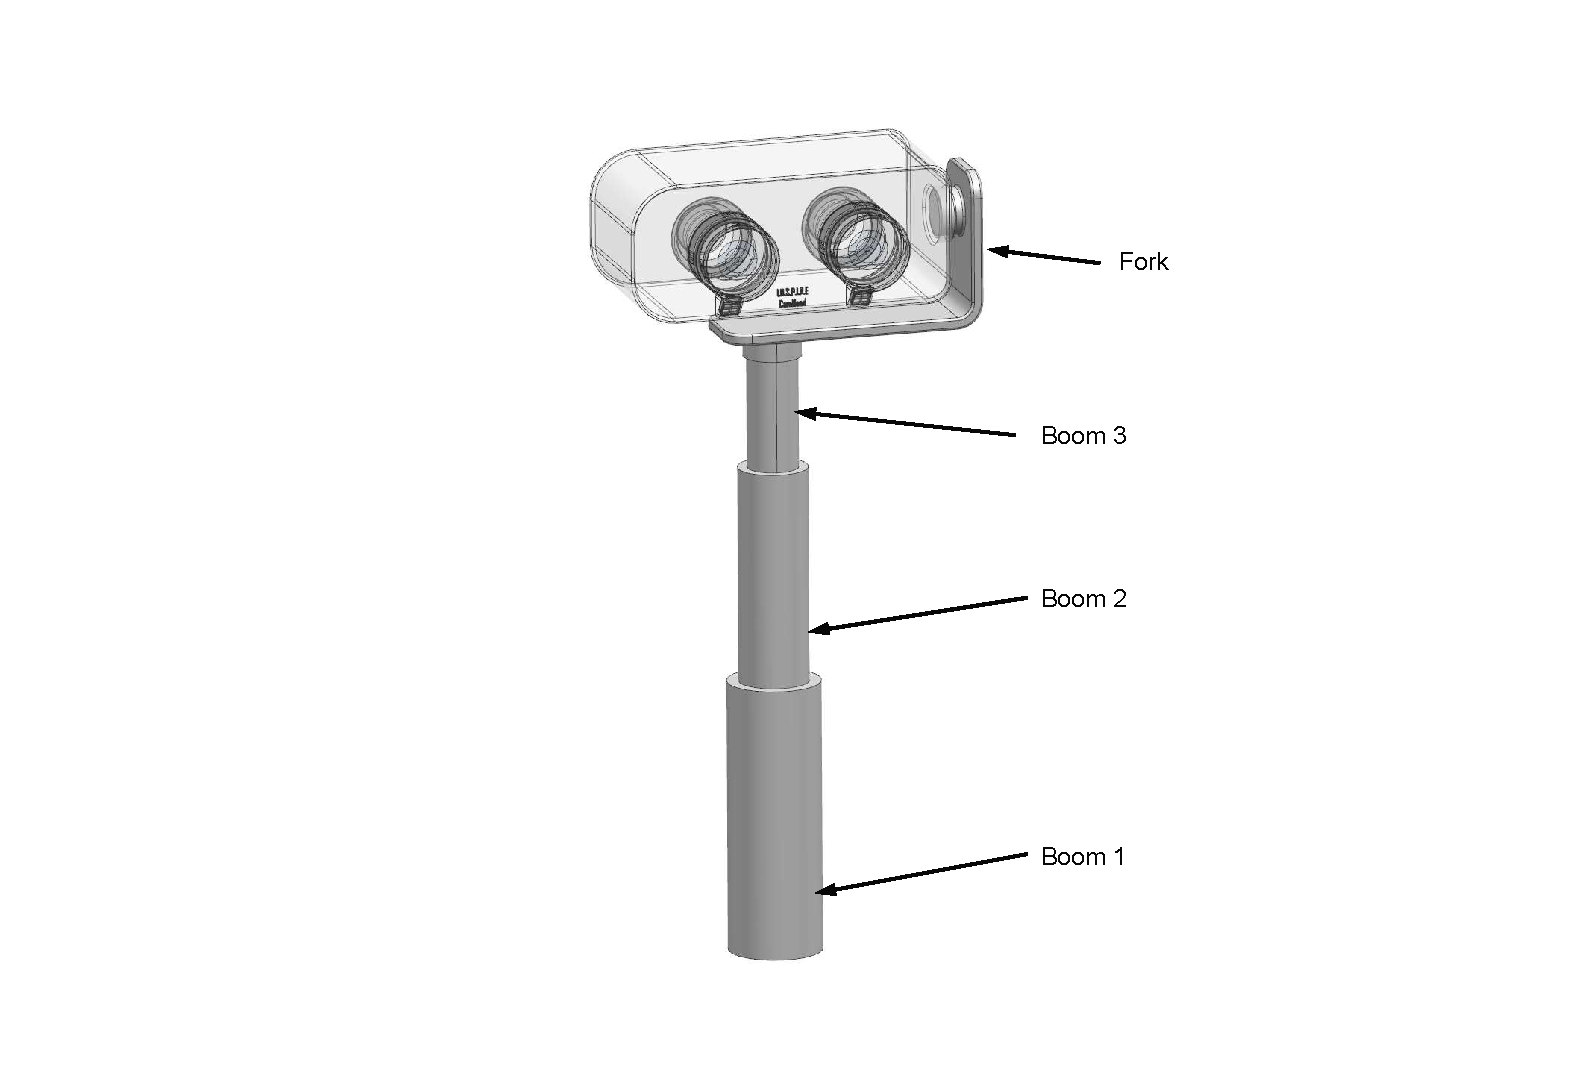
\includegraphics[width=0.25\textwidth]{Media/tcs_con_boom}}}}  \\[1em]
		& & & &  \\
		\multicolumn{2}{l}{$CON_6= \left( \frac{1}{CON_{B1}} +\frac{1}{CON_{B2}}+\frac{1}{CON_{B3}}+\frac{1}{CON_{F}} \right)^{-1} $} & & & \\[2em]
		\multicolumn{2}{l}{$CON_6= 7.10 \cdot 10^{-2}\ \frac{\W}{\K}$} & & &  \\[8em]
		\hline
		Part &  Cross section & Length  & Material & Amount \\ \hline
		& & & & \\[-0.75em]
		Boom 1 & $S_{B1}= 181 \ \mm^2$ & $l_{B1}=116 \ \mm$ & Aluminium & 1 \\[0.5em]
		Boom 2 & $S_{B2}= 134 \ \mm^2$ & $ll_{B2}=95 \ \mm$ & Aluminium & 1 \\[0.5em]
		Boom 3 & $S_{B3}= 97 \ \mm^2$ & $l_{B3}= 60\ \mm$ & Aluminium & 1 \\[0.5em]
		Fork & $S_{F}= 200\ \mm^2$ & $l_{F}=170\ \mm$ & Aluminium & 1 \\
		\label{tab:tcs_nodes2}
	\end{tabular}
\end{table}	

\begin{table}[htb]
\centering
\caption{Definition of heat conductance $CON=\frac{1}{R}$ between the nodes according to \autoref{fig:tcs_network}.}
\begin{tabular}{l@{\qquad}cccc}		
		\hline
		Name &  Linked Components &  \multicolumn{3}{c}{Geometry}\\ \hline
		& & & & \\[-0.5em]
		\textbf{Suspension} & \textbf{Chassis} $\leftrightarrow$ \textbf{Node$_1$}  &  \multicolumn{3}{c}{\multirow{2}{*}{\adjustbox{valign=t}{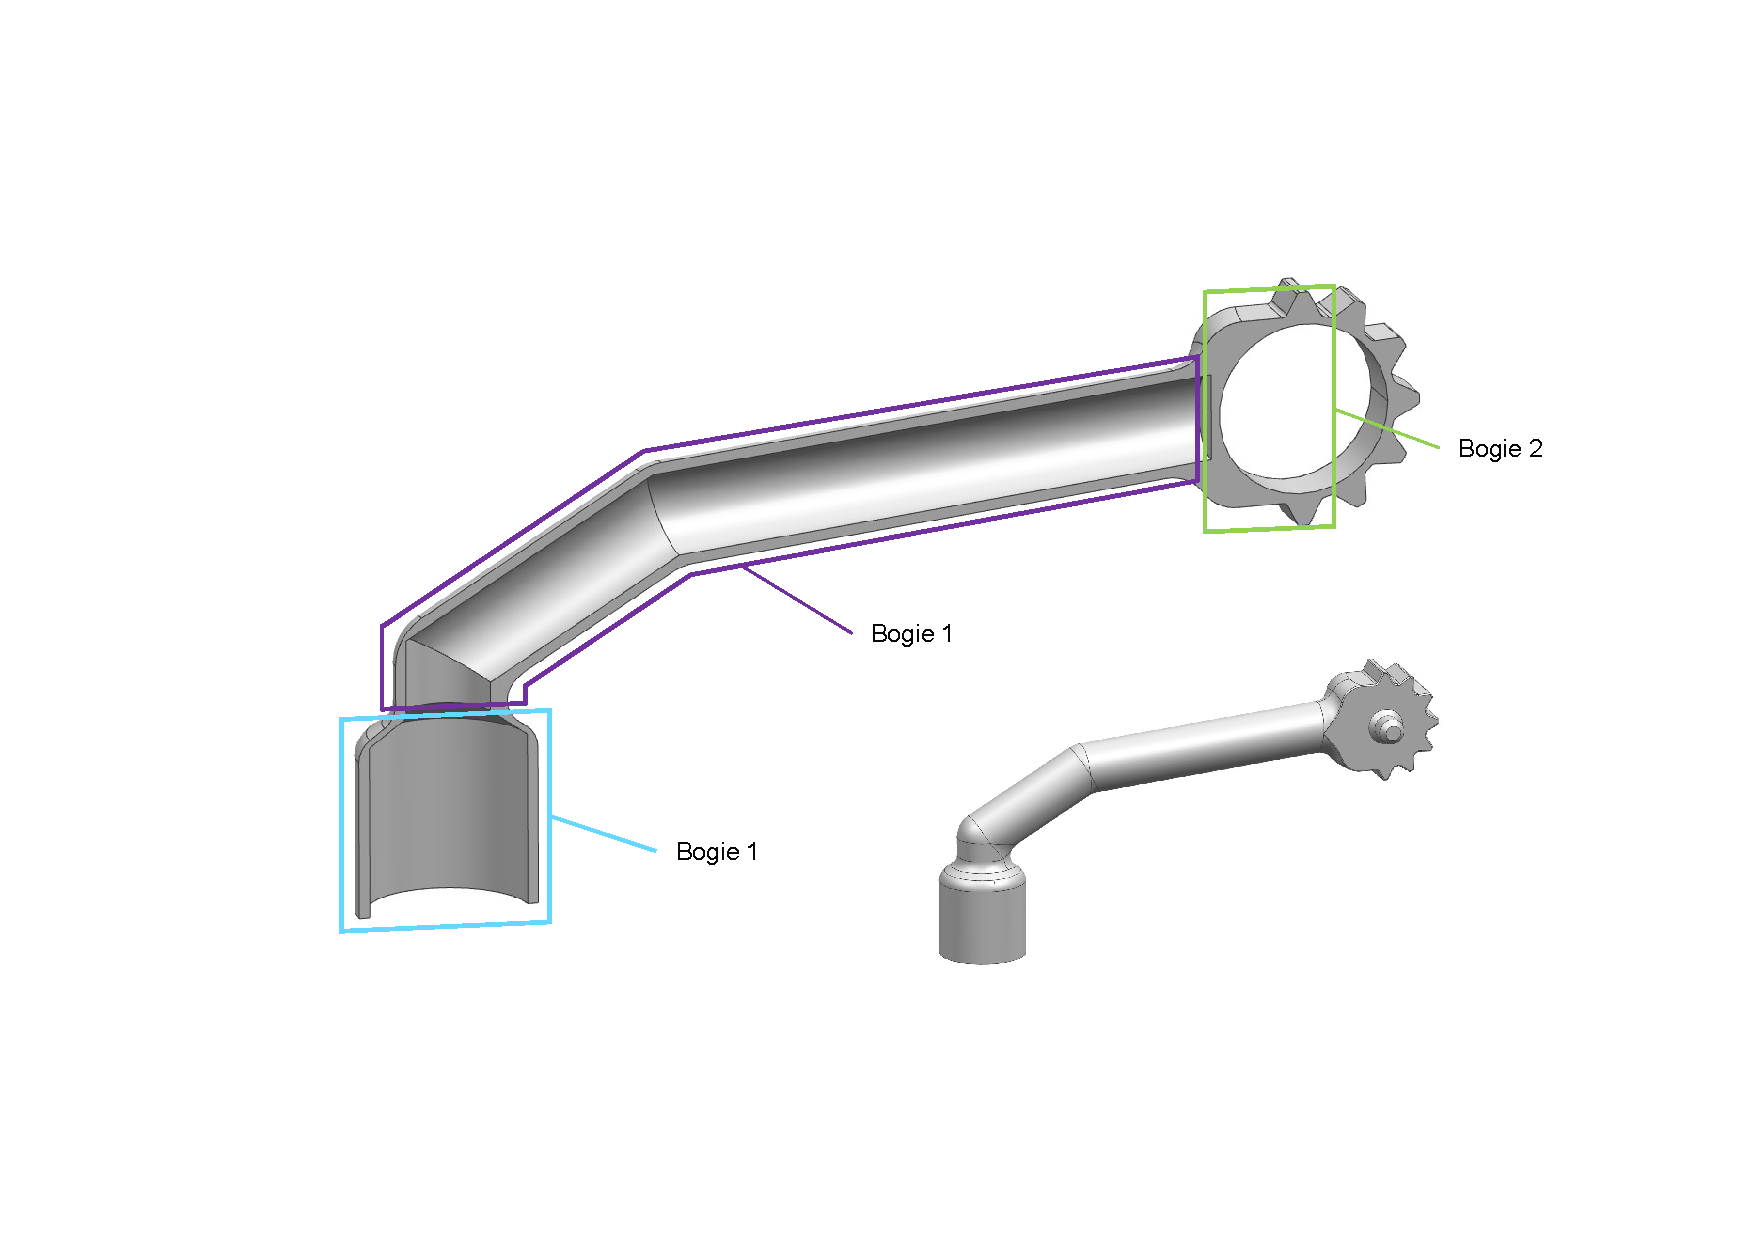
\includegraphics[width=0.455\textwidth]{Media/tcs_con_bogie}}}}  \\[1em]
		& & & &  \\
		\multicolumn{2}{l}{$CON_7=\left( \frac{1}{CON_{B1}} +\frac{1}{CON_{B2}}+\frac{1}{CON_{B3}}\right)^{-1}$} & & & \\[1em]
		\multicolumn{2}{l}{$CON_7= 1.30 \cdot 10^{-1}\ \frac{\W}{\K}$} & & & \\[6em]
		
		\hline
		Part &  Cross section & Length  & Material & Amount \\ \hline
		& & & & \\[-0.75em]
		Bogie 1 & $S_{B1}=275 \ \mm^2$ & $t_{B1}=20\ \mm$ & Aluminium & 1 \\[0.5em]
		Bogie 2 & $S_{B2}=113 \ \mm^2$ & $t_{B2}=162\ \mm$ & Aluminium & 1 \\[0.5em]
		Bogie 3 & $S_{B3}=201 \ \mm^2$ & $t_{B3}=37\ \mm$ & Aluminium & 1 \\[5em]		

		\hline
		Name &  Linked Components &  \multicolumn{3}{c}{Geometry}\\ \hline
		& & & & \\[-0.75em]
		\textbf{Mounting} & \textbf{Steer Engine} $\leftrightarrow$ \textbf{Node$_1$}  &  \multicolumn{3}{c}{\multirow{2}{*}{\adjustbox{valign=t}{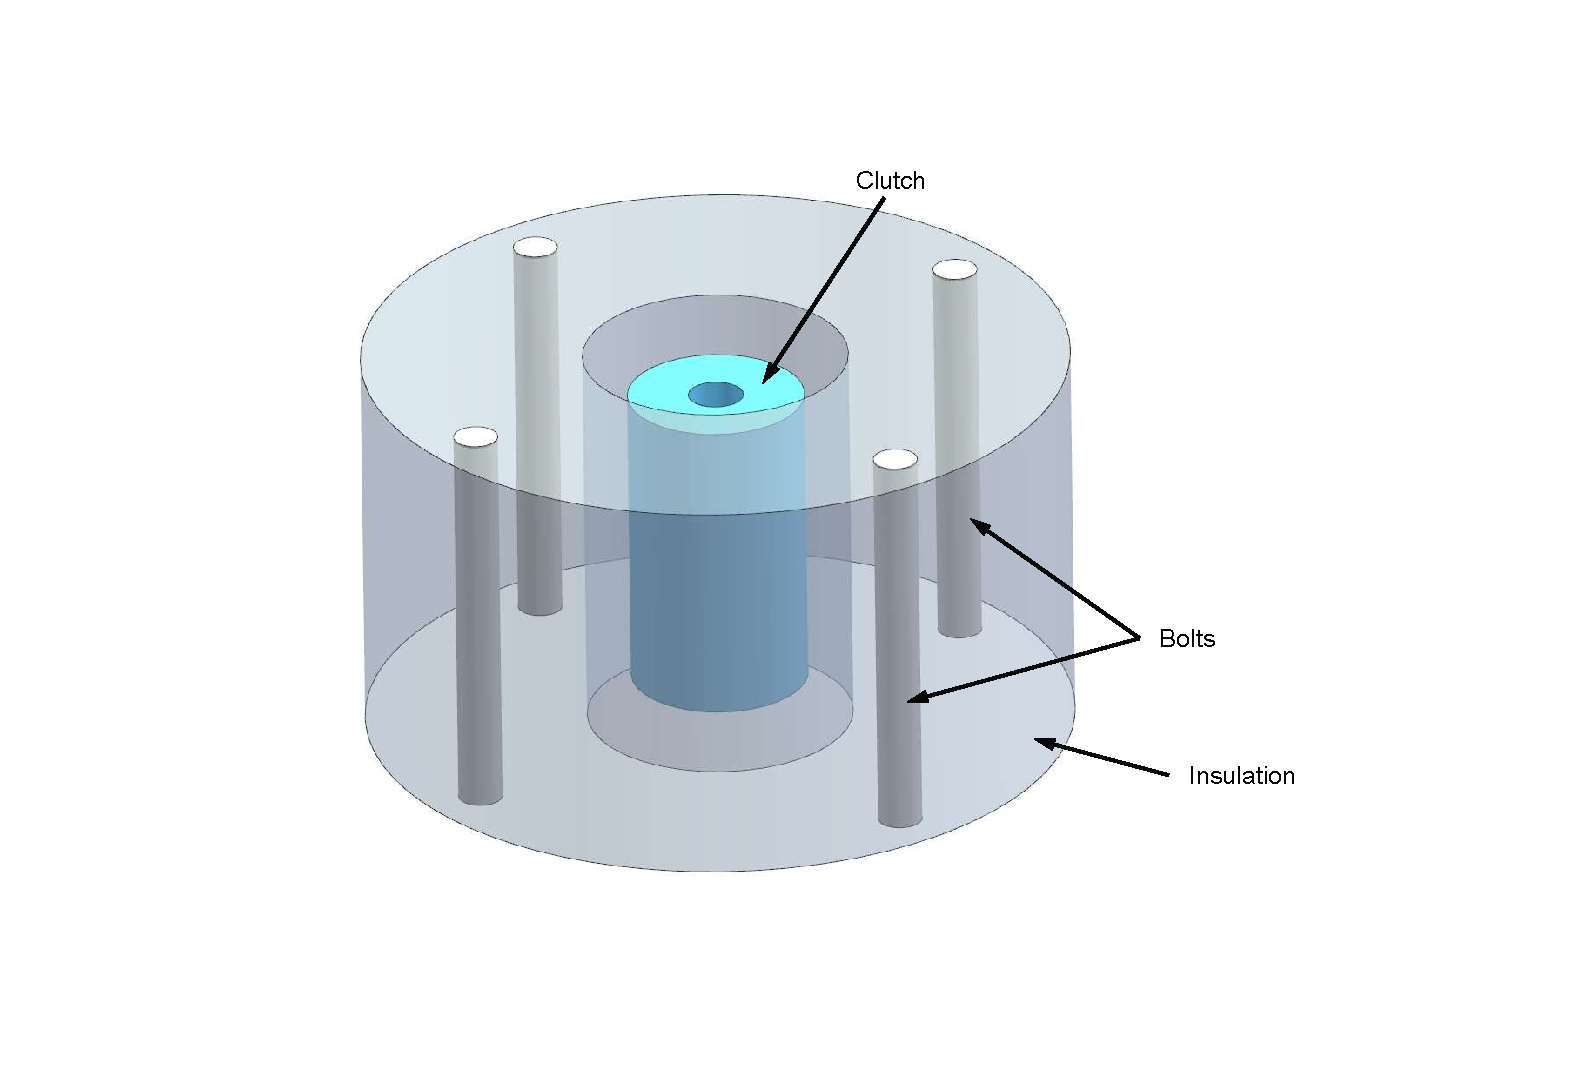
\includegraphics[width=0.4\textwidth]{Media/tcs_con_steer}}}}  \\[1em]
		& & & &  \\
		\multicolumn{2}{l}{$CON_8=CON_C+CON_I+n_B\cdot CON_B  $} & & & \\[2em]
		\multicolumn{2}{l}{$CON_8= 6.85\cdot 10^{-1}\ \frac{\W}{\K}$} & & &  \\[6em]
		\hline
		Part &  Cross section & Thickness  & Material & Amount \\ \hline
		& & & & \\[-0.75em]
		Clutch & $S_{C}= 45.4 \ \mm^2$ & $t_{C}=14 \ \mm$ & Aluminium  & 1 \\[0.5em]
		Insulation & $S_{I}= 691 \ \mm^2$ & $t_{I}=18 \ \mm$ & Aerogel & 1 \\[0.5em]
		Bolts & $S_{B}= 3.14 \ \mm^2$ & $t_{B}= 18\ \mm$ & Steel & 4 \\
		\hline
		\label{tab:tcs_nodes3}
	\end{tabular}
\end{table}	


\begin{table}[htb]
	\centering
	\caption{Definition of heat conductance $CON=\frac{1}{R}$ between the nodes according to \autoref{fig:tcs_network}.}
	\begin{tabular}{l@{\qquad}cccc}		
		Name &  Linked Components &  \multicolumn{3}{c}{Geometry}\\ \hline
		& & & & \\[-0.5em]
		\textbf{Wheel Fork} & \textbf{Node$_1$} $\leftrightarrow$ \textbf{Node$_2$}  &  \multicolumn{3}{c}{\multirow{2}{*}{\adjustbox{valign=t}{\includegraphics[width=0.45\textwidth]{Media/tcs_con_fork}}}}  \\[1em]
		& & & &  \\
		\multicolumn{2}{l}{$CON_{10}=\left( \frac{1}{CON_{F1}} +\frac{1}{CON_{F2}}\right)^{-1} $} & & & \\[1em]
		\multicolumn{2}{l}{$CON_{10}= 1.46 \cdot 10^{-1}\ \frac{\W}{\K}$} & & & \\[8em]
		
		\hline
		Part &  Cross section & Length  & Material & Amount \\ \hline
		& & & & \\[-0.75em]
		Fork 1& $S_{F1}=200 \ \mm^2$ & $l_{F1}=175$ & Aluminium & 1 \\[0.5em]	
		Fork 1& $S_{F2}=200 \ \mm^2$ & $l_{F2}=175$ & Aluminium & 1 \\[5em]	

		\hline
		Name &  Linked Components &  \multicolumn{3}{c}{Geometry}\\ \hline
		& & & & \\[-0.5em]
		\textbf{Mounting} & \textbf{Drive Engine} $\leftrightarrow$ \textbf{Node$_2$}  &  \multicolumn{3}{c}{\multirow{2}{*}{\adjustbox{valign=t}{\includegraphics[width=0.5\textwidth]{Media/tcs_con_drive}}}}  \\[1em]
		& & & &  \\
		\multicolumn{2}{l}{$CON_{11}=  \left( \frac{1}{CON_G} +\frac{1}{CON_S+CON_I+n_B\cdot CON_B} \right)^{-1} $} & & & \\[2em]
		\multicolumn{2}{l}{$CON_{11}= 2.19 \cdot 10^{-1}\ \frac{\W}{\K}$} & & & \\[5em]
		
		\hline
		Part &  Cross section & Thickness  & Material & Amount \\ \hline
		& & & & \\[-0.75em]
		Gear Box & $S_{G}= 566 \ \mm^2$ & $t_{G}= 43.1\ \mm$ & Steel & 1 \\[0.5em]
		Shaft & $S_{S}= 23.8 \ \mm^2$ & $t_{S}=8 \ \mm$ & Steel & 1 \\[0.5em]
		Insulation & $S_{I}=490  \ \mm^2$ & $t_{I}=8 \ \mm$ & Aerogel  & 1 \\[0.5em]
		Bolts, M3 & $S_{B}=7.07  \ \mm^2$ & $t_{B}= 8\ \mm$ & Steel  & 4 \\[5em]	
	\end{tabular}
\label{tab:tcs_nodes4}
\end{table}	

\clearpage

\begin{table}[htb]
	\centering
	\caption{Definition of heat conductance $CON=\frac{1}{R}$ between the nodes according to \autoref{fig:tcs_network}.}
	\begin{tabular}{l@{\qquad}cccc}		
		\hline
		Name &  Linked Components &  \multicolumn{3}{c}{Geometry}\\ \hline
		& & & & \\[-0.5em]
		\textbf{Rim} & \textbf{Node$_2$} $\leftrightarrow$ \textbf{Ground}  &  \multicolumn{3}{c}{\multirow{2}{*}{\adjustbox{valign=t}{\includegraphics[width=0.3\textwidth]{Media/tcs_con_rim}}}}  \\[1em]
		& & & &  \\
		\multicolumn{2}{l}{$CON_{13}= 5.11 \cdot 10^{-3}\ \frac{\W}{\K}$} & & & \\[7em]
		
		\hline
		Part &  Cross section & Length  & Material & Amount \\ \hline
		& & & & \\[-0.75em]
		Rim & $S_R=12 \ \mm^2$ & $l_r=100\ \mm$ & Aluminium & 6 \\[1.5em]
		\multicolumn{5}{l}{\textit{Note}: It was assumed that the wheel temperature equals the surface temperature} \\
		\multicolumn{5}{l}{because of the thin rims and resulting low heat conduction.} \\
	\end{tabular}
\label{tab:tcs_nodes5}
\end{table}

\subsection{Heat switch} \label{sec:app_therm_3}

The characteristic of the switch conductance depends on the mean temperature $T_M$, shown by measurements in cite .
As this temperature won´t be calculated in the analysis, the corresponding component temperature $T_C$ shall be used.
In order to describe the characteristic, it was divided in three sections, \autoref{fig:tcs_switch03}.
The temperature where the disk decouples is $T_{toggle}=108 K$ and not applicable for the current application.
By reducing the height, the toggle temperature can be increased and the characteristic can be shifted to higher temperatures ("to the right").
It was assumed that the gradients of section 2 and 3 as well as the temperature range of section 2 keep constant.
The axis interception is a function the toggle temperature ($a_2=f(\Delta T_{toggle}),\ \Delta T_{Toggle}=T_{new}-T_{old}|_{toggle}$).
The used toggle temperature are listed in autoref

\begin{table}[H]
	\centering
	\caption{Toggle temperature and amount of bi-metallic heat switch.}
	\begin{tabular}{c@{\quad}ccc}
		\toprule
		Heat switch name  & Linked Components & Temperature  & Amount \\ \midrule
		$CON_{S1}$ & {Camera} $\leftrightarrow$ {Radiator} & -20\ $^\circ$C  & $n_{S1}=$4  \\[1em]
		$CON_{S2}$ & {EBay} $\leftrightarrow$ {Chassis} & -30\ $^\circ$C  & $n_{S2}=$2  \\[1em]
		$CON_{S3}$ & {Drive Engine} $\leftrightarrow$ {Node$_2$} & -20\ $^\circ$C  & $n_{S3}=1$  \\
		&											&						& (in total 4)  \\ \bottomrule
	\end{tabular}
	\label{tab:tcs_toggle}
\end{table}


\begin{table}[H]
	\centering
	\caption{Sections and range of the switch characteristic.}
	\begin{tabular}{c@{\qquad}rcl@{\qquad}l}
		\toprule
		Section & \multicolumn{3}{l}{Temperature range} & Heat conductance $CON_S= \frac{1}{R_t}$ \\ \midrule
		& & & &  \\[-0.5em]
		1 & $T_{toggle} >$ & $ T_C  $ & & $CON_{S}= 16.4 \cdot 10^{-3}\ \frac{\W}{\m^2 \K} = const.$\\[1.5em]
		2 & $T_{toggle}\leq$ & $ T_C $ & $ < T_1$ & $CON_{S} (T_C) = a_{1.1} \cdot T_C+ a_{1.2}$\\[1em]
		& & & & $a_{1.1}= +1.272\cdot 10^{-3}\ \frac{\W}{\m^2 \K^2}$ \\[1em]
		& & & & $  a_{1.2}= -1.272\cdot 10^{-3}\ \frac{\W}{\m^2 \K^2}\cdot \Delta T_{Toggle}-0.117\ \frac{\W}{\m^2 \K}$  \\[2em]
		3 & & 	$ T_C$ & $^ > T_1$ & $CON_{S}(T_C) = a_{2.1} \cdot T_C+ a_{2.2}$\\[1em]
		& & & & $a_{2.1}=+ 333\cdot 10^{-6}\ \frac{\W}{\m^2 \K^2}$ \\[1em]
		& & & & $  a_{2.2}= -333\cdot 10^{-6}\ \frac{\W}{\m^2 \K^2}\cdot \Delta T_{Toggle}-28.3 \cdot 10^{-3}\ \frac{\W}{\m^2 \K}$  \\[1em] \bottomrule
	\end{tabular}
	\label{tab:tcs_section}
\end{table}

\begin{figure}[htb]
	\centering
	\includegraphics[width=1\textwidth]{Media/tcs_diag_section}
	\caption{Conductance characteristic of heat switch diveded in sections.}
	\label{fig:tcs_switch03}
\end{figure}

\subsection{Rover absorptivity} \label{sec:app_therm_4}
The rover position relative to the direct sun radiation is given by the ecliptic longitude $\lambda_R$ and latitude $\delta_R$ angle, where the axis $x_E$ points always to the sun, \autoref{fig:tcs_rad2}.
The amount of solar radiation $S_0$ absorbed by the rover surfaces depends on the sun altitude and can be determined by the view factor $\varphi$, see \autoref{fig:tcs_rad1}.
The view factors during the eclipse are set to zero.

\begin{table}[H]
	\begin{tabular}{l@{\qquad}ll}
		View Factor 1,& horizontal surface:& $ \varphi_1=\cos (\lambda_R) \cdot \cos (\delta_R)  $ \\
		View Factor 2, & vertical surface: &$ \varphi_2=\cos (90^{\circ}-\lambda_R) \cdot \cos (\delta_R)  $\\
	\end{tabular}
\end{table}

\begin{figure}[h]
	\centering
	\subfloat[View factor depending on the absorption surface.]{\includegraphics[height=0.4\textwidth]{Media/tcs_rover_rad}\label{fig:tcs_rad1}}\qquad\qquad
	\subfloat[Definition of ecliptic longitude $\lambda_R$ and latitude $\delta_R$ of the rover on Europa.]{\includegraphics[height=0.3\textwidth]{Media/tcs_angle.png}\label{fig:tcs_rad2}}
	\caption{Bi-metallic heat switch, \cite{ref_tcs_04}.}
	\label{fig:tcs_rad}
\end{figure}


\subsection{Input Values} \label{sec:app_therm_5}
\begin{table}[H]
	\centering
	\caption{Temperatur limits of the rover components.}
	\begin{tabular}{l@{\qquad\qquad}cc}
		\toprule 
		& \multicolumn{2}{l}{Temperature limits in [$^\circ$C]} \\ 
		Component	&	min. & max. \\ \midrule
		OBC & -55 & 70 \\
		Transmitter & -10 & 50 \\
		Receiver & -30 & 70  \\
		PCDU & -40 & 60  \\
		Battery & -20 & 60 \\
		Camera & -40 & 70  \\
		Objektive  & -40 & 71  \\
		Steering Engine & -30 & 100 \\
		Drive Engine & -40 & 100 \\
		Drive Gear & -40 & 100  \\ \bottomrule
	\end{tabular}
	\label{tab:tcs_limits}
\end{table}

\begin{figure}[H] 
	\centering
	\includegraphics[width=0.8\textwidth]{Media/tcs_lynx_calc}
	\caption{Digitalised \cite{ref_tcs_01} and calculated heat conduction in comparison.}
	\label{fig:tcs_lynx}
\end{figure}
The characteristic of the \textit{LyNX}\textsuperscript{\tiny\textregistered} conduction was approximated with following function,
\begin{equation}
\lambda(T)= \left(1.76 \cdot 10^{-4}\ \frac{\W}{\m \K^4} \cdot T^3 -2.37\cdot 10^{-1}\ \frac{\W}{\m \K^3} \cdot T^2 +79.5 \frac{\W}{\m \K^2} \cdot T -5.55\cdot 10^{3}\ \frac{\W}{\m \K}\right) \cdot f_{r}  
\label{eq:tcs_lynx}
\end{equation}
with the reduction factor $f_{r}$=0.8.

\begin{table}[H]
	\centering
	\caption{Dimensions of the thermal straps \textit{LyNX}\textsuperscript{\tiny\textregistered}.}
	\begin{tabular}{l@{\quad}cc}
		\toprule
		Linked Components & Cross section  & Length$^{1)}$  \\ \midrule
		EBay $\leftrightarrow$ RTG & 42\ mm$^2$ & 230 mm  \\[0.25em] 
		Drill $\leftrightarrow$ RTG &10 \ mm$^2$ &345 \ mm \\[0.25em] 
		Steer Engine $\leftrightarrow$ RTG & 36\ mm$^2$&644\ mm  \\[0.25em] 
		Drive Engine $\leftrightarrow$ RTG &42 \ mm$^2$&897\ mm  \\[0.25em] \bottomrule
		& &   \\[-0.5em]
		\multicolumn{3}{l}{$^{1)}$\ Du to uncertainties the length was increased about 15\%.}\\[1em]
	\end{tabular}
	\label{tab:tcs_lynx}
\end{table}

The Europa surface temperature varies at the  equator between $T_{e,min}=80~\K$ and\\ $T_{e,max}=130~\K$, depending on the sun inclination.
The temperature at the pole is ${T_{Pole}=50~\K}$, \cite{Europa}.
It was assumed that the surface temperature depends on the sun altitude.
A trigonometrical interpolation was defined as follows.
\[ T_{Surface}(\lambda, \delta) = T_{Pole} + \cos (\delta) \cdot [(T_{e,min}+\cos (\lambda)\cdot (T_{e,max}-T_{e,min}))-T_{Pole}] \]
For $\lambda$ and $\delta$ see \autoref{sec:app_therm_4}.\\

\begin{table}[H]
	\centering
	\caption{Minimum and maximum of surface emissivity and absorptivity values, \cite{ref_tcs_05}.}
	\begin{tabular}{l@{\qquad\qquad}cc@{\qquad\qquad}cc}
		\toprule
		& \multicolumn{2}{l}{Emissivity [-]} & \multicolumn{2}{l}{Absorptivity [-]}  \\ 
		Surface finishing	&	min. & max. 	&	min. & max.   \\\midrule
		Aluminium, polished & &0.05  & & 0.2   \\
		Aluminium, sand blasted & &0.2  & & 0.4   \\
		White paint & 0.8 & 0.9 & 0.2 & 0.5  \\ \bottomrule
		& & & & \\
	\end{tabular}
	\label{tab:tcs_surface}
\end{table}


\begin{table}[H]
	\centering
	\caption{Heat conductivity in $\frac{\W}{\m \K}$}
	\begin{tabular}{l@{\qquad\qquad}c@{\qquad\qquad}c@{\qquad\qquad}l}
		\toprule
		Material & Nominal & Used & Source \\ \midrule
		Aerogel & 0.002 - 0.05 & 0.05 & \cite{ref_tcs_03} \\
		Aluminium$^{1)}$  & 110 - 220 & 220 & \cite{ref_tcs_10}, \cite{ref_tcs_11}, \cite{ref_tcs_12} \\
		Steel$^{1)}$ & 15 - 43 & 45 & \cite{ref_tcs_08}, \cite{ref_tcs_09} \\ 
		Titan  & 7.1  & 7.1 & \cite{ref_tcs_06}, \cite{ref_tcs_07} \\\bottomrule
		&&&\\[-0.75em]
		\multicolumn{4}{l}{\small{$^{1)}$\  Depends on the alloying component, a conservative value was choosen.}}\\
	\end{tabular}
	\label{tab:tcs_conduct2}
\end{table}

\begin{table}[H]
	\centering
	\caption{Radiation surface and finishing of components.}
	\begin{tabular}{l@{\qquad}l@{\qquad}ll}
		\toprule
		Part  & Surface [$\m^2$] & Finishing & Note \\ \midrule
		Chassis - top/bottom & $S_{Ch1}=0.086$ &  white paint & for albedo\\
		Chassis - side & $S_{Ch2}=0.081$ &  white paint & for albedo\\
		Chassis - total & $S_{Ch3}=0.423$ &  white paint & for emissivity\\
		RTG& $S_{RTG}=0.086$ & white paint & konstant emissivity of 0.9\\
		Electric Bay& $S_{Bay}=0.146$ & AL, sand blastet & \\
		Camera - housing & $S_{Cam}=0.027$ & AL, sand blastet &\\
		Camera - radiator & $S_{Rad}=0.066$ & white paint &  \\
		Steer Engine& $S_{E,S}=0.002$ & white paint& \\
		Drive Engine& $S_{E,D}=0.003$ &white paint & \\
		Bogie & $S_{B}=0.018$ &white paint & \\
		Wheel Fork& $S_{F}=0.008$ &white paint & \\ \bottomrule
		&&& \\
		\multicolumn{3}{l}{The cross sections were taken form the CAD model.}
	\end{tabular}
	\label{tab:tcs_surf}
\end{table}

\clearpage

\setcounter{figure}{0}
\setcounter{table}{0}

\section{Radiation}

\label{sec:AppendixRadiation}

In this chapter, detailed calculations are performed on which \autoref{sec:Radiation} is based on. All calculations and figures in \autoref{sec:AppendixRadiation} are performed with SPENVIS unless otherwise stated. In order to simulate the radiation on Europa an orbit around Jupiter is simulated with the orbit parameters of Europa with a total mission duration of 30 days. The chosen parameters were an perijove altitude of 664,862 km, an apojove altitude of 676,938 km, and an inclination of 0.47°.

\subsection{Jupiters Radiation Environment}

\label{subsec:AppendixRadiationEnvironment}

In order to compare the radiation environment around Jupiter and the radiation environment around Earth the following trapped radiation models were used: for Jupiter the D\&G83+Salammbo proton model and D\&G83+GIRE+SalammboE electron model was used; for Earth the AP-8 proton model and the AE-8 electron model was used.

\begin{figure}[htb]
     \centering
     \begin{subfigure}[b]{0.49\textwidth}
         \centering
         \includegraphics[width=\textwidth]{Media/E_Electron_Flux}
         \caption{Average spectra of trapped electrons around Earth}
         \label{fig:trappedelectronsEarth}
     \end{subfigure}
     \hfill
     \begin{subfigure}[b]{0.49\textwidth}
         \centering
         \includegraphics[width=\textwidth]{Media/E_Proton_Flux}
         \caption{Average spectra of trapped protons around Earth}
         \label{fig:trappedprotonsEarth}
     \end{subfigure}
     \hfill
     \begin{subfigure}[b]{0.49\textwidth}
         \centering
         \includegraphics[width=\textwidth]{Media/J_Electron_Flux}
         \caption{Average spectra of trapped electrons around Jupiter}
         \label{fig:trappedelectronsJupiter}
     \end{subfigure}
     \hfill
     \begin{subfigure}[b]{0.49\textwidth}
         \centering
         \includegraphics[width=\textwidth]{Media/J_Proton_Flux}
         \caption{Average spectra of trapped protons around Jupiter}
         \label{fig:trappedprotonsJupiter}
     \end{subfigure}
     \caption{Average trapped proton and electron fluxes on an orbit around earth at 25,000 km, through the outer Van Allen radiation belt, and on Europa's orbit around Jupiter.}
     \label{fig:trappedprotonelectronfluxes}
\end{figure}

\clearpage

\subsection{Radiation Exposures}

\label{subsec:AppendixRadiationExposures}

In order to simulate the TID for different radiation protections the Geant4 tool Multi-Layered Shielding Simulation (MULASSIS) is used. As target material silicon is selected with a thickness of 1 \(\mu \text{m}\). As shape a planar slap is selected because of the ice ground on one side of the rover.

\begin{figure}[htb]
     \centering
     \begin{subfigure}[b]{0.49\textwidth}
         \centering
         \includegraphics[width=\textwidth]{Media/J_Electron_Shielding}
         \caption{TID for Electrons as Source Particles}
         \label{fig:TIDElectronShielding}
     \end{subfigure}
     \hfill
     \begin{subfigure}[b]{0.49\textwidth}
         \centering
         \includegraphics[width=\textwidth]{Media/J_Proton_Shielding}
         \caption{TID for Protons as Source Particles}
         \label{fig:TIDProtonShielding}
     \end{subfigure}
     \caption{TID of aluminium, titanium, and the optimised radiation structure shown in \autoref{tab:OptimalRadiationProtection} with a weight target of all three structures of 0.5 \(\text{g/cm}^2\) over 30 days of exposure on Europa.}
     \label{fig:AluminiumTitanOptimised}
\end{figure}

\begin{table}[htb]
\centering
\caption{Used components and the respective radiation tolerance and location}
\begin{adjustbox}{max width=\textwidth}
\begin{tabular}[l]{lccccc}

	\toprule
		Components	&	Rated TID	&	Exposed TID	&	Location\\
	\midrule
	
	BLDC Motors	&	-	&	< 205	&	locomotion housing\\	
	
	Stepper Motors	&	100 000	&	< 205	&	locomotion housing\\
	
	Harness	&	-	&	< 98	&	chassis\\	
	
	Stereo Vision Cams	&	40	&	< 31	&	camera housing\\	
	
	OBC	&	1 000	&	< 17	&	E-Bay\\
	
	PCDU	&	20	&	< 17	&	E-Bay\\
	
	Transmitter	&	20	&	< 17	&	E-Bay\\
	
	Receiver	&	20	&	< 17	&	E-Bay\\
	
	Battery	&	20	&	< 17	&	E-Bay\\
	
	Housekeeping Board	&	\(\approx\) 20	&	< 17	&	E-Bay\\
	
	IMU	&	\(\approx\) 20	&	< 17	&	E-Bay\\
	
	Multiplexer	&	\(\approx\) 20	&	< 17	&	E-Bay\\
	
	Ground Radar	&	\(\approx\) 20	&	< 17	&	E-Bay\\
	
	Sun Sensor	&	10 000	&	2 000	&	outside rover\\
	
	Camera Lenses	&	10 000	&	2 000	&	outside rover\\

	\bottomrule

\end{tabular}
\end{adjustbox}
\label{tab:RadiationList}
\end{table}

\begin{figure}[htb]
     \centering
     \begin{subfigure}[b]{0.49\textwidth}
         \centering
         \includegraphics[width=\textwidth]{Media/J_Electron_Compartments}
         \caption{TID for Electrons as Source Particles}
         \label{fig:TIDElectronShielding}
     \end{subfigure}
     \hfill
     \begin{subfigure}[b]{0.49\textwidth}
         \centering
         \includegraphics[width=\textwidth]{Media/J_Proton_Compartments}
         \caption{TID for Proton as Source Particles}
         \label{fig:TIDProtonShielding}
     \end{subfigure}
     \caption{TID for different compartments as seen in \autoref{fig:RadiationOverview}. The E-Bay is shielded by 4 mm aluminium, 0.415 mm lead, and 0.033 mm iron; the camera compartment by 2 mm aluminium, 0.415 mm lead, and 0.033 mm iron; the chassis by 2 mm aluminium; the electric motors by 1 mm aluminium.}
     \label{fig:CompartmentTID}
\end{figure}

\newpage

\subsection{Improvements}

\label{app:AppendixRadiationImprovements}

All simulations of the improvements introduced in \autoref{subsec:RadiationImprovements} are performed in the same way as in \autoref{subsec:AppendixRadiationExposures}. \\ \\
In \autoref{fig:Radiation_Improvements_Individual}, the TID over 30 days within the E-Bay is shown. If all components with a radiation resistance under 43.27 krad are shielded individually, the additional shielding structure around the E-Bay can be removed and the aluminium structure would be sufficient.

\begin{figure}[htp]
	\centering
	\includegraphics[width=0.7\textwidth]{Media/J_Improvements_Individual}
	\caption{TID with 4 mm Al shielding over a mission duration of 30 days}
	\label{fig:Radiation_Improvements_Individual}
\end{figure}

The resulting mass savings can be calculated with \autoref{eq:RadiationImprovementsIndividual} with \(m^*\) as the specific weight of the radiation protection and \(N\) as the amount of components within the E-Bay with a radiation resistance under 43.27~krad as of \autoref{tab:RadiationList}.

\begin{equation}
	\Delta m = SA_\text{E-Bay} \cdot m^*_\text{Shielding} - \sum\nolimits_{n=0}^N SA_\text{Component, n} \cdot m^*_\text{Shielding}
	\label{eq:RadiationImprovementsIndividual}
\end{equation}

With inserted values this results in a mass saving of \(\Delta m\) = 736.2~g.

\begin{figure}[htp]
	\centering
	\includegraphics[width=0.7\textwidth]{Media/J_Improvements_Ice}
	\caption{TID with 4 mm Al shielding and 1 cm of Water over a mission duration of 30 days}
	\label{fig:Radiation_Improvements_Ice}
\end{figure}

\clearpage

\setcounter{figure}{0}
\setcounter{table}{0}

%-----------------------------------------------------------
\section{Digital Appendix}		\label{app:DigitalAppendix}
%-----------------------------------------------------------

\begin{table}[htb]
	\centering
	\begin{tabular}{llcc}
	\toprule
		Name  & Path & Type & Size  \\
	\midrule
		TCS Analysis final & 300 Thermal\ & Exle Sheet with Macros, *.xlsm & 326 kB  \\
	\bottomrule
	\end{tabular}
	\caption{Digital Appendix}
	\label{app:DigitalAppendix}
\end{table}

\cleardoublepage
\end{document}







% Formatierungsoptionen & Dokumenteneinstellungen

%\documentclass[11pt,a4paper,twoside]{report}
%\usepackage[a4paper,left=2.5cm,right=2.5cm, top=2.4cm, bottom=3.2cm]{geometry}
%\usepackage[hang]{caption}
%\usepackage[font={small}]{caption}
%%\usepackage{ucs}
%\usepackage[utf8]{inputenc}
%% Standard Style-Files
%\usepackage{amsmath,amssymb,amsthm}
%\usepackage{a4}
%\usepackage[table,xcdraw]{xcolor}
%\usepackage{graphicx}
%\usepackage{algorithmic,algorithm}
%%\usepackage{subfigure}
%\usepackage{longtable}
%\usepackage[makeroom]{cancel}
%\usepackage[]{placeins}
%\usepackage{adjustbox}
%%Textbox: \begin{textblock*}{29mm}(45mm,80mm)-> h:45mm v:80 von oberen linken Ecke mit 29mm Breite, Höhe durch Inhalt. %Inhalt beliebig(Bilder,Text,..) 
%\usepackage[absolute]{textpos}
%\usepackage{caption}
%\usepackage{lipsum} 
%\usepackage[hidelinks, linktoc = all]{hyperref}
%\usepackage{multirow}
%\usepackage{lscape}
%%\usepackage[official]{eurosym}
%\usepackage[gen]{eurosym}
%\usepackage{subcaption}
%%\usepackage{subfig}
%\usepackage{pdfpages}
%%\usepackage{url}
%\usepackage{listings}
%\usepackage[sorting=none, backend=bibtex, maxbibnames=99, url=true]{biblatex}
%%\usepackage{url}
%%\bibliographystyle{unsrt}
%\usepackage{color} %red, green, blue, yellow, cyan, magenta, black, white
%\definecolor{mygreen}{RGB}{28,172,0} % color values Red, Green, Blue
%\definecolor{mylilas}{RGB}{170,55,241}
%\addbibresource{References}
%
%\interfootnotelinepenalty=10000
%
%\lstset{language=Matlab,%
%	basicstyle=\linespread{0.5}\tiny],
%    %basicstyle=\color{red},
%    breaklines=true,%
%    morekeywords={matlab2tikz},
%    keywordstyle=\color{blue},%
%    morekeywords=[2]{1}, keywordstyle=[2]{\color{black}},
%    identifierstyle=\color{black},%
%    stringstyle=\color{mylilas},
%    commentstyle=\color{mygreen},%
%    showstringspaces=false,%without this there will be a symbol in the places where there is a space
%    numbers=left,%
%    numberstyle={\tiny \color{black}},% size of the numbers
%    numbersep=7pt, % this defines how far the numbers are from the text
%    emph=[1]{for,end,break},emphstyle=[1]\color{red}, %some words to emphasise
%    %emph=[2]{word1,word2}, emphstyle=[2]{style}, 
%    extendedchars=true,
%    literate={µ}{{$\mu$}}1 {η}{{$\eta$}}1 {²}{{$^{2}$}}1 {µm}{{$\mu$m}}1 {µm'}{{$\mu$m '}}1 {μ}{{$\mu$}}1 {π}{{$\pi$}}1 {±}{{$\pm$}}1 ,   
%}
%% ############################################################################
%% Inverse Suche mit xdvi und kile:
%%
%\usepackage{srcltx}
%%
%% 1) xdvi starten mit 
%%    > xdvi -editor 'kile %f --line %l' bericht.dvi
%% 2) Bei einem Klick ins angezeigte dvi-Dokument springt kile automatisch an
%%    die richtige Stelle im latex-file
%
% 
%% Seitenstil
%\pagestyle{headings}
%
%% Abstand zwischen Abs"atzen
%\setlength{\parskip}{1.5ex}
%
%% Einr"uckung der ersten Zeile eines Absatzes unterdr"ucken
%\setlength{\parindent}{0pt}
%
%% Grosszuegigere Wortabstaende
%\sloppy
%
%% Damit Bilder m"oglichst da sind, wo man sie will
%\setcounter{topnumber}{20}
%\setcounter{bottomnumber}{20}
%\setcounter{totalnumber}{20}
%\renewcommand{\topfraction}{.9999}
%\renewcommand{\bottomfraction}{.9999}
%\renewcommand{\textfraction}{0}
%
%
%\newcommand{\chapquoteright}[3]{\begin{quotation} \textit{#1} \end{quotation} \begin{flushright} - #2, \textit{#3}\end{flushright} }
%
%\newcommand{\chapquoteleft}[3]{  \begin{quotation} \textit{#1} \end{quotation} \begin{flushleft}- #2, \textit{#3}\end{flushleft} }
%
%%##########################################################################
%% Bilder:
%% ps/eps-File mit Unterschrift:
%\newcommand{\mypicture}[4]{
%\begin{figure}[hptb]
%\begin{center}
%\includegraphics[scale=1,angle=#4]{#1}
%\caption{#2}\label{#3}
%\end{center}
%\end{figure}
%}%newcommand%
%% Aufruf mit \mypicture{file}{caption}{label}{angle}
%
%% ps/eps-File mit Unterschrift und Angabe der Breite:
%\newcommand{\myscalepicture}[5]{
%\begin{figure}[hptb]
%\begin{center}
%\includegraphics[width=#5,angle=#4]{#1}
%\caption{#2}\label{#3}
%\end{center}
%\end{figure}
%}%newcommand%
%% Aufruf mit \myscalepicture{file}{caption}{label}{angle}{width}
%
%%##########################################################################
%% Tabellen:
%% Gleitende Tabelle:
%\newcommand{\mytable}[3]{
%\begin{table}[hptb]
% \caption{#2}
%  \centerline{#1}
%  \label{#3}
%\end{table}
%}%newcommand%
%% Aufruf mit \mytable{tabelle}{caption}{label}
%
%
%
%%##########################################################################
%% Gleichungs--Referenzen:
%
%% im Text
%\newcommand{\refeqn}[1]{(\ref{#1})}
%% Aufruf mit \refeqn{label}
%
%%##########################################################################
%% Wort-Abkuerzungen:
%
%% \def\abkuerzung/{{text}}
%% Aufruf mit \abkuerzung/
%\def\MKS/{{Mehrk"orpersystem}}
%
%
%%##########################################################################
%% Textmodus
%%##########################################################################
%% Mathematischer Modus 
%
%% Masseinheiten
%\newcommand{\meh}[1]{~\mbox{#1}}
%% Aufruf mit \meh{einheit}
%% Zahlenmengen
%\newcommand{\realR}{{\Bbb{R}}}
%\newcommand{\integerN}{{\Bbb{N}}}
%\newcommand{\complexC}{{\Bbb{C}}}
%
%\newcommand{\fett}[1]{{\mathbf{#1}}}
%% Aufruf mit \realR, \integerN und \complexC
%
%
%%##########################################################################
%% Sonderumgebungen
%\newtheorem{definition}{Definition}[chapter]
%% Aufruf mit \begin{definition}[zusatz]  text  \end{definition}
%\newtheorem{satz}{Satz}[chapter]
%% Aufruf mit \begin{satz}[zusatz]  text  \end{satz}
%
%\theoremstyle{definition}
%\newtheorem{beispiel}{Beispiel}[chapter]
%% Aufruf mit \begin{beispiel}[zusatz]  text  \end{beispiel}
%\newtheorem{algorithmus}{Algorithmus}[chapter]
%% Aufruf mit \begin{algorithmus}[zusatz]  text  \end{algorithmus}
%\floatstyle{ruled}
%\newfloat{algorithm}{thp}{alg} 
%\floatname{algorithm}{Algorithmus}
%
%%###########################################################################
%% Bearbeitung von einzelnen Kapiteln
%
%%\includeonly{02Mission}
%
%%###########################################################################
%
%\begin{document}
%
%%###########################################################################
%
%   Titelseite
%
%###########################################################################

\begin{titlepage}
	
	\begin{textblock*}{117mm}(56mm,30mm)
	%{127mm}(51mm,47mm)
		
		\begin{center}
		
		
			72320 Roversystemtechnik \\
			Summer Semester 2021
			
			
			\vspace{20mm}
			
			\large \textbf{INSPIRE} \\ 
			\vspace{5mm}
			\large \textbf{IN-situ Sampling and Primal Investigation \\ Rover on Europa}
			
			\vspace{20mm}
			
			\large \textbf{Phase 0/A-Study of a Rover Mission on the Surface \\ of the Jupiter moon Europa}
			
			\begin{figure}[htb]
    		\centering
     		\includegraphics[width=\textwidth]{Media/Logo}
			\end{figure}
			
			\normalsize 
			Denis Acker \\
			Daniel Bölke \\
			Korbinian Kasper \\
			Christian Korn \\
			Nicolas Probst \\
			Saskia Sütterlin \\
			
			
			\vspace{10mm}
			
			Supervisors: \\
			Moritz Nitz M.Sc. \\
			Patrick Winterhalder M.Sc. 
			
			\vspace{10mm}
			
			University of Stuttgart \\
			Institute of Space Systems \\
			Prof. Dr. Sabine Klinkner \\
			18.07.2021
			
		\end{center}
	
	\end{textblock*}
	
\end{titlepage}



%bericht no IRS-16-035

%  \vspace{10mm} 
%         {\large \hspace{13mm} \\
%         \large \hspace{13mm} \\
%         \large \hspace{13mm} \\
%         \large \hspace{13mm} 72320 Roversystemtechnik\\
%         \centering 
%         \hspace{13mm} Summer Semester 2021\\   }
%  \vspace{10mm}
%
%         {\Large
%          \bf
%          \hspace{20mm} Phase 0/A-Study of a Rover Mission \\} 
%         {\Large
%          \bf
%          \hspace{20mm} on the surface of the Jupiter moon:\\
%          } 
%         {\Large
%          \bf
%          \hspace{20mm} Europa: INSPIRE\\
%          }
% 
%
%  \vspace{30mm}
%         {\large \hspace{20mm}Saskia Sütterlin}\\       
%         {\large \hspace{20mm}Denis Acker}\\
%         {\large \hspace{20mm}Krobinian Kasper}\\
%         {\large \hspace{20mm}Daniel Bölke}\\
%         {\large \hspace{20mm}Nicolas Probst}\\    
%         {\large \hspace{20mm}Christian Korn}\\
%  \vspace{20mm}
%  \makebox[40mm]{\large \hspace{16mm} Supervisor: }\makebox[65mm][l]
%                                   {\large\ Moritz Nitz M.Sc.}
%  \makebox[40mm]{}\makebox[65mm][l]{\large\ Patrick Winterhalder M.Sc.}\\
%
%  \vspace{20mm}
%         {\large \hspace{20mm} University of Stuttgart} \\
%         {\large \hspace{20mm} Institute of Space Systems }\\
%         {\large \hspace{20mm} Prof.\ Dr.\ Sabine Klinkner}\\
%  \vspace{10mm}       
%         {\large \hspace{20mm} 18.07.2021}
%         
%         
%\end{center}
%\end{titlepage}
%
%\clearpage
%\thispagestyle{empty}
%\cleardoublepage
% hier zitat
%*\newpage

%%\textit{\chapquoteright{''Sometimes it was hard to believe that all this had been carried up into space and assembled here five hundred miles above the Earth. I didn't know, until Tim mentioned it casually, that most of the material in the Station had actually come from the Moon. The Moon's low gravity made it much more economical to ship equipment from there instead of from the Earth - despite the fact that Earth was so much closer.''}{Arthur C. Clarke}{Roy Malcolm in Islands in the Sky -- 1952}
%%\begin{figure*}[htb]
%{\centering
%\captionsetup{width=0.8\textwidth}
%\includegraphics[width=0.8\textwidth]{Pictures/LumadiCoverComposite}
%\caption{Lunar massdriver composite image. Footage from Apollo 8 and Apollo 11. Rendering of lunar massdriver 3D models.}
%}
%\end{figure*}
%\FloatBarrier

%\vfill
%\chapquoteright{''Denken Sie groß!''}{Deichkind}{2015}}




%% Inhalt auf der rechten Seite beginnen
%
%
%\strut
%\clearpage
%\thispagestyle{empty}
%\cleardoublepage
%  
%\evensidemargin=2pt
%\oddsidemargin=2pt
%
%
%
%% Zeilenabstand strecken
%\renewcommand{\baselinestretch}{1}\normalsize
%\pagenumbering{roman}
%
%\chapter*{Symbols}

\addcontentsline{toc}{chapter}{Symbols}

\markboth{}{SYMBOLS}

\renewcommand{\arraystretch}{1.2}

\begin{longtable}[l]{lll}

	\textbf{Symbol}	&	\textbf{Definition}	\hspace{8cm}	&	\textbf{Unit}	\\ \\
	
% Latin Symbols

\(a\)					&	Constant for the Geometry of a Porous Media	& nm							\\
\(A\)					&	Wheel Ground Contact Area					& m								\\
\(b_\text{w}\)			&	Wheel Width 								& m								\\
\(c\)					&	Coefficient of Soil Cohesion				& Pa							\\
$C_\text{batt,req}$		&	Total Required Battery Capacity				& Wh							\\
$C_\text{batt,req}$		&	Battery Nominal Capacity					& Wh							\\
$C_\text{cell}$			&	Cell Voltage								& V								\\
$CON_*$					&	Heat conductance of concerning component	& $\frac{\W}{\K}$				\\
\(C_\text{rr}\)			&	Rolling Resistance Coefficient					& -								\\	
\(d\)					&	Wheel Distance Vertical						& m								\\
\(d_\text{w}\)			&	Wheel Diameter								& m								\\
$DoD$					&	Depth of Discharge							& $\%$							\\
\(DP\)					&	Drawbar Pull								& N								\\
\(H\)					&	Soil Thrust									& N								\\
\(h_\text{ice}\)		&	Ice Crust Surface Thickness on Europa		&	m							\\
\(k_\text{c}\)			&	Sinkage Modulus								& \(\frac{\text{kN}}{\text{m}^{n+2}}\) \\
\(k_\phi\)				&	Soil Friction Angle Sinkage Modulus			& \(\frac{\text{kN}}{\text{m}^{n+3}}\) \\
\(l_\text{w}\)			&	Wheel Ground Contact Length					& m								\\
\(l\)					&	Wheel Distance Length						& m								\\
$R_t$					&	Heat resistance								& $\frac{\K}{\W}$				\\
\(T_\text{surface}\)	&	Surface Temperature on Europa				&	K							\\
$M$						&	Number of Cells in Parallel					& -								\\
\(MMP\)					& 	Mean Maximum Pressure 						& kPa							\\
$m_\text{RTG}$			&	RTG Mass									& kg							\\
\(m_\text{w}\)			&	Weight per Wheel							& kg							\\
\(n\)					&	Soil Deformation Exponent					& -								\\
$N$						&	Number of Cells in Series					& -								\\
\(P\)					&	Wheel Electrical  Power						& W								\\
$P_\text{el}$			&	RTG Electrical Power						& $W_\text{el}$					\\
$P_\text{el,req}$		&	Required Electrical Power					& $W_\text{el}$					\\
$P_\text{mode}$			&	Demanded Electrical Power per Mode			& $W_\text{el}$					\\
$\dot{Q}$				&	Heat flow									& W								\\
	$S_0$					&	Solar constant 							& $\frac{\W}{\m^2}$				\\
\(R_\text{b}\)			&	Bulldozing Resistance						& N								\\
\(R_\text{c}\)			&	Compaction Resistance						& N								\\
\(R_\text{g}\)			&	Gravitational Resistance					& N								\\
\(R_\text{r}\)			&	Rolling Resistance							& N								\\
\(R_\text{total}\)		&	Total Resistance							& N								\\
\(S\)					&	Radiation surface							& m$^2$							\\
$t_\text{e}$			&	Mode Duration								& s								\\
\(v\)					&	Velocity									& \(\frac{\text{m}}{\text{s}}\)	\\
\(W\)					&	Normal Force 								& N								\\
\(W_\text{w}\)			&	Normal Force per Wheel						& N								\\
\(z\)					&	Sinking Depth								& m								\\


%Greek Symbols

$\alpha$				&	Absorptivity								& -  							\\
$\alpha_\text{BOL}$		&	BOL Specific Power							& $\frac{W_{el}}{kg}$			\\
\(\delta\)				&	Wheel Deflection							& m								\\
$\delta_\text{R}$		&	Ecliptic latitude of the rover on Europa	& $\circ$						\\
\(\epsilon\)			&	Emissivity 									&	-							\\
$\eta_\text{LiIon}$		&	Efficiency of LiIon Cells					& -								\\
$\lambda$				&	Heat conductivity							& $\frac{\W}{\m \K}$			\\
$\lambda_\text{R}$		&	Ecliptic longitude of the rover on Europa	& $\circ$						\\
\(\Phi\)				&	Friction Angle								& deg							\\
$\varphi$				&	View factor									& -								\\
\(\rho_\text{E}\)		&	Albedo of Europa			  				& -								\\
\(\rho_\text{ice}\)		&	Inner Encoder Ring Diameter  				&	\(\frac{\text{kg}}{m^3}\)	\\
$\sigma_\text{b}$ 		&	Stefan-Boltzmann constant					& $\frac{\W}{\m^2\K^4}$ 		\\
\(\theta\)				&	Slope Angle									& deg							\\
\(\tau\)				&	Torque										& Nm							\\




\end{longtable}

\chapter*{Abbreviations}
\addcontentsline{toc}{chapter}{Abbreviations}

\markboth{}{ABBREVIATIONS}

\begin{longtable}[l]{ll}

2D		& Two Dimensional \\
3D		& Three Dimensional \\
APXS	& Alpha Particle X-Ray Spectrometer \\
BER		& Bit Error Rate \\
BLDC	& Brushless Direct Current	\\
BOL     & Begin of Life \\
BOM     & Begin of Mission \\
COMM    & Communications \\
COTS	& Commercial of the Shelf \\
C\&DH	& Command \& Data Handling \\
CPU		& Core Processing Unit \\
DoD     & Depth of Discharge \\
EOM     & End of Mission \\
EPS     & Electrical Power System \\
FEC		& Forward Error Correction \\
GPR		& Ground Penetrating Radar \\
HGA	    & High Gain Antenna \\
IRS     & Institute of space Systems at the University of Stuttgart \\
INSPIRE & IN-situ Sampling and Primal Investigation Rover on Europa \\
JUICE 	& Jupiter Icy Moons Explorer \\
LGA		& Low Gain Antenna \\		
PCDU    & Power Control and Distribution Unit \\
PCU     & Power Control Unit \\
PDU     & Power Distribution and Control Unit \\
IMU     & Inertial Measurement Unit \\
ESA		& European Space Agency	\\
MP		& Mobility Package \\
NASA    &   National Aeronautics and Space Administration \\
SPENVIS	&	SPace ENVironment Information System	\\
HPC     & High Priority Commands \\
RHU		& Radioisotope Heater Unit\\
RTG     & Radioisotope Thermoelectric Generator \\
eMMRTG  & Enhanced Multi Mission Radioisotope Thermoelectric Generator \\
eSMMRTG & Enhanced and Scaled Multi Mission Radioisotope Thermoelectric Generator (3kg) \\
TID		& Total Ionizing Dose \\
TRIPLE 	& Technologies for Rapid Ice Penetration and Subglacial Lake Exploration \\
TRL     & Technology Readiness Level \\
OBC		& On-Board Computer \\
S/C     & Spacecraft\\
SBC		& Single Board Computer \\



\end{longtable}

\cleardoublepage






%\addcontentsline{toc}{chapter}{Symbols}
%
%\markboth{}{SYMBOLS}
%
%\renewcommand{\arraystretch}{1.2}
%
%\begin{longtable}[l]{lll}
%  $a$                      & nm                                        & Constant for the Geometry of a Porous Media   \\
%$h_\text{Ice}$           & $\text{km}$,$\text{m}$                      & Ice Crust Surface Thickness on Europa         \\
%$T_\text{Surface}$       & $K$                                         & Surface Temperature on Europa                 \\
%$\epsilon$               & -                                           & Emissivity                                    \\
%$\rho_\text{Ice}$       & $\frac{\text{kg}}{m^3}$                      & Inner Encoder Ring Diameter                   \\
%   
%
%\label{tab:my-table}\\
%\end{longtable}
%
%
%
%
%\chapter*{Abbreviations}
%\addcontentsline{toc}{chapter}{Abbreviations}
%
%\markboth{}{ABBREVIATIONS}
%
%\begin{table}[htb]
%\begin{tabular}[l]{ll}
%PCDU    & Power Control and Distribution Unit \\
%BOL     & Begin of Life \\
%BOM     & Begin of Mission \\
%EOM     & End of Mission \\
%2D		& Two Dimensional \\
%3D		& Three Dimensional \\
%PCU     & Power Control Unit \\
%PDU     & Power Distribution and Control Unit \\
%EPS     & Electrical Power System \\
%IMU     & Inertial Measurement Unit \\
%IRS     & Institute of space Systems at the University of Stuttgart \\
%ESA		&	European Space Agency	\\
%NASA    &   National Aeronautics and Space Administration \\
%SPENVIS	&	SPace ENVironment Information System	\\
%RTG     & Radioisotope Thermoelectric Generator \\
%eMMRTG  & Enhanced Multi Mission Radioisotope Thermoelectric Generator \\
%eSMMRTG & Enhanced and Scaled Multi Mission Radioisotope Thermoelectric Generator (3kg) \\
%TID		& Total Ionizing Dose \\
%
%\end{tabular}
%\end{table}

\cleardoublepage
%%###########################################################################
%
%   Inhaltsverzeichnis
%
%   (wird automatisch erstellt; dieser File ist nicht zu ändern)
%
%###########################################################################
\tableofcontents
\listoffigures
\listoftables



%
%
%\pagenumbering{arabic}
%%###########################################################################
%
%   Einleitung
%
%###########################################################################
%
\chapter{The Mission}
\label{chap:mission}

During the observation  of Jupiter, the Glileo spacecraft did also some flybys of the Jupiter moons, \cite{Mission_01}.
The scientist gahtered data from Europa, which suported the evidence of a thick icy surface.
The possibility of liquid water underneath lead astrobiologists to the assumption that extraterrestrial life could exist on Europa, \cite{Mission_02}.
That is why Europo is - beside Mars - an interesting object of research.\\

Therefore, the ESA will launch the \textit{JUICE} oriber in 2022 to investigate Europa in more detail, \cite{Mission_03}. 
But also the NASA is developing  \textit{Europa Clipper} to get detailed information.
Additionally, they plan a lander for Europer to bring scientific instruments onto the surface. \cite{Mission_04} \cite{Mission_05}.
%There is a side mission planed DLR will perform the side mission \textsc{Technologies for Rapid Ice Penetration and Subglacial Lake Exploration}, with project coordinator Dr. Waldmann, which will take samples of the water by melting through the ice with an special testing probe.\\

Under the leadership of  Prof. Dr.-Ing. Klinkner, the Institute of Aero Space Systems started within a seminar a feasibility study about a rover system to explore Europa surface, which shall  be part of the \textit{TRIPLE} mission.
This challenge was given to five student teams in order to develop concepts, construct preliminary designs, perform analysis and make evaluations to  meet the mission objectives and fit the mandatory requirements cite. \\


This report contain the results of the Phase A study of the rover system \textsc{IN-situ Sampling and Primal Investigation Rover on Europa}  (INSPIRE).
%\chapter{Operation}
\label{chap:Operation}
.....

\section{Mission Phases}
For the INSPIRE Mission Phase 0 study five basic mission phases have been defined. Furthermore a sixed optional mission phase after the nominal mission lifetime has been established which will be conducted if the rover is still operational after its nominal lifetime.

\begin{itemize}
\itemsep0pt
\item	\textbf{Phase 0:} Launch and Flight Phase
\item	\textbf{Phase 1:} Entry, Descent and Landing Phase
\item	\textbf{Phase 2:} Depolyment Phase
\item	\textbf{Phase 3:} Egress, Comissioning and Early Operation Phase
\item	\textbf{Phase 4:} Mission Operation Phase
\item	(\textbf{Phase 5:} Exceeding Mission Operation Phase) 
\end{itemize}

\begin{figure}[H]
{\centering
\includegraphics[width=1.0\textwidth]{Media/timeline}
\caption{Preliminary Mission Timeline for INSPIRE.}
\label{fig:timeline}
}
\end{figure}


Based on these missions phases some preliminary rover system modes as well as a basic mission timeline were concluded.

\subsection{Rover System Modes}
For this case study several rover system modes were defined. All ten modes are listed in \autoref{tab:systemmod}. 

They are seperated into two groups. The design critical modes are displayed in white and are defined as system modes, which significantly influence the preliminary design of the rover subsystem like the thermal or power subsystem. None design critical modes (grey) also have a major influence on multiple subsystems of the rover but play a secondary role in the thermal and power budget of the rover for this Phase 0 study. These non design critical modes extend from the rover storage and launch until the finale deployment of the rover is completed. These modes and their design options depend heavily on the final design of the lander with which INSPIRE flies to Europe. Therefore, a clear definition of such modes is not possible at this time in the course of this phase 0 study. However, the respective considerations, preferences and options have been briefly described in the mode descriptions. It is important to note that INSPIRE's goal is to provide a flexible rover design with as few hard requirements as possible for the parent lander. Therefore, many aspects of the rover, as well as the none design critical modes, will need to be further defined and elaborated in later phases of the project in close consultation with the customer. \\
For example, the exact interfaces between rover and lander should be defined in more detail. Depending on the subsequently chosen interfaces, many possibilities may arise in the corresponding rover system modes. With an appropriate interface, for example, the excess electrical and thermal energy of the RTG, which is already active during the flight, could be used to supply the lander system with heat and power. A corresponding interface could also enable the transmission of health checks from INSPIRE. \\
The deployment phase will strongly depend on the final design of the lander, INSPIRE's position within the lander and also the possibilities that the lander provides to INSPIRE.
Possible deployment strategies would be as follows:

\begin{itemize}
\itemsep0pt
\item	\textbf{Option 1:} If INSPIRE on ground level: Release from storage box through spring mechanism or actuators. Rover storage configuration allows rolling and possible motorized actuation
\item	\textbf{Option 2:} If INSPIRE is above ground level: Similar as Option 1 but an additonal ramp and ramp deployment would be required.
\item	\textbf{Option 3:} INSPIRE will be deployed through the landers robotic arm if it is capable of lifting its mass.
\end{itemize}


% Please add the following required packages to your document preamble:
% \usepackage{graphicx}
% \usepackage[table,xcdraw]{xcolor}
% If you use beamer only pass "xcolor=table" option, i.e. \documentclass[xcolor=table]{beamer}
\begin{table}[H]
\centering
\resizebox{\textwidth}{!}{%
\begin{tabular}{|c|c|c|l|}
\hline
Number & Rover System Modes                  & Abbrevation & \multicolumn{1}{c|}{Definition}                                                                                                                                                                                                                                                                                                                                                                                                                                                                                                                                                                                                   \\ \hline
\rowcolor[HTML]{EFEFEF} 
0      & Launch/Off Mode                     & OFF         & \begin{tabular}[c]{@{}l@{}}From Launch until EDL Phase\\ Rover System is OFF\\ Exact mode description t.b.d. and can be adapted to meet the lander demands\\ Health tests on Occasion during flight time are foreseen (PCDU could be active)\\ Batteries on Storage Capacity at launch and may be recharged on occasion (like Rosetta Mission)\\ Telemetry data shall be sent by the Lander (optional if possible)   \\ RTG on =\textgreater Electrical and Thermal Power may be used \\ (for Lander Power and Thermal Systems) or is disposed of by shunts\end{tabular}                                                          \\ \hline
\rowcolor[HTML]{EFEFEF} 
1      & Entry, Descent and Landing          & EDL         & \begin{tabular}[c]{@{}l@{}}From Entry until next morning after secure landing of Lander on Europa\\ See Mode OFF\\ PCDU ON after secure landing (Powered by RTG)\\ Heaters ON (powered by remaining RTG Power)\\ Battery charging if no Kill Switch is used\end{tabular}                                                                                                                                                                                                                                                                                                                                                          \\ \hline
\rowcolor[HTML]{EFEFEF} 
2      & Deployment and Early Operation Mode & EOP         & \begin{tabular}[c]{@{}l@{}}First Morning after EDL\\ Exact mode description t.b.d. and can be customized to lander \\ =\textgreater Dependant on final Lander Design\\ Critical Deployments (Egress System) and leaving the lander\\ Optional whether Kill Switch ejected =\textgreater Battery charging can start\\ Rover System Activation possibilities: Kill Switch, Lander Interface, HPC from Earth\\ PCDU ON\\ OBC ON\\ Heaters ON\\ After sufficient Battery Capacity is reached (50\%): Deployment of Rover Boogie \\ and checkout/health check of all Rover Systems\\ Afterward switching to Charging Mode\end{tabular} \\ \hline
3      & Idle/ Perception                    & ID          & \begin{tabular}[c]{@{}l@{}}During Idle Operation Time\\ Rover powered by RTG or Batteries (Excess Power charges Batteries)\\ PCDU ON\\ All Components in Standby or Power Saving Mode if possible\\ Stereovision Camera ON for Orientation and Observation (Science Data)\\ Hazcams and OBC ON for Orientation and Path Analysation\\ COMM ON for larger time intervals (Listening Mode)\end{tabular}                                                                                                                                                                                                                             \\ \hline
4      & Safe Mode/ Hibernation (SAFE)       & SAFE        & \begin{tabular}[c]{@{}l@{}}Entered in case of emergency or contingency Rover    \\ Survival Mode =\textgreater Minimum Power\\ PCDU ON  \\ COMM sends Emergency Signal then switches to\\ COMM ON for small time intervals (Listening Mode)\\ OBC OFF until Command received =\textgreater High Power Commands (HPC)\\ Heaters ON\\ Science data shall be stored without data loss\\ Applicable during Day and Nighttime\\ Exit after receiving the corresponding command\\ (Optional: Timer ON and Restart of Rover System after time period has passed)\end{tabular}                                                            \\ \hline
6      & Communication                       & COMM        & \begin{tabular}[c]{@{}l@{}}During Transmission of major Telemetry or Science Data\\ Rover powered by RTG or Batteries (Excess Power charges Batteries)\\ PCDU ON\\ All Components in Standby or Power Saving Mode if possible\\ OBC SB\\ COMM ON (Transmission Mode)\end{tabular}                                                                                                                                                                                                                                                                                                                                                 \\ \hline
7      & Charging                            & BAT         & \begin{tabular}[c]{@{}l@{}}For Battery charging\\ Rover batteries charged by RTG\\ PCDU ON\\ All Components in Standby or Power Saving Mode if possible\\ OBC SB\\ Quit after sufficient charge is reached\end{tabular}                                                                                                                                                                                                                                                                                                                                                                                                           \\ \hline
8      & Locomotion                          & LOC         & \begin{tabular}[c]{@{}l@{}}For Rover Movement and Observation\\ Locomotion and Navigation ON\\ Hazcams and Traversing Path Analysis ON\\ OBC ON\\ PCDU ON\\ COMM OFF\\ Stereovision Camera ON for Orientation and Observation (Science Data)\\ Only during Daytime\end{tabular}                                                                                                                                                                                                                                                                                                                                                   \\ \hline
9      & Payload Observation Mode            & OBS         & \begin{tabular}[c]{@{}l@{}}Payload Mode for Science Data Collection during Daytime\\ OBC ON\\ PCDU ON   \\ COMM OFF\\ Stereovision Camera ON for Orientation and Observation (Science Data)\\ RADAR ON for Ground Investigation =\textgreater Drill Location\\ Only during Daytime\end{tabular}                                                                                                                                                                                                                                                                                                                                   \\ \hline
10     & Payload: Ice Core Mode              & ICE         & \begin{tabular}[c]{@{}l@{}}Payload Mode for   Science Data Collection during Daytime or Nighttime\\ OBC ON\\ PCDU ON\\ COMM OFF\\ Ice Core Drill ON during Ice   Core Sample Collection\\ Afterwards Sample will be   analysed =\textgreater APXS ON\end{tabular}                                                                                                                                                                                                                                                                                                                                                                 \\ \hline
\end{tabular}%
}
\caption{Collection of Rover System Modes. [Kommt noch in Anhang]}
\label{tab:systemmod}
\end{table}

%\chapter{Subsystems}
\label{chap:subsystems}
.....



\section{Rover}
\label{sec:rover}
...
\section{Structure and Mechanics}
\label{sec:mechanics}
...
\section{Communications and Command and Data-Handling}
\label{sec:comm}
...
\section{Payload}
\label{sec:payload}
...
\clearpage
%-------------------------------------------------------------------------------
\section{Thermal Control System} \label{sec:thermalcontrol}
%-------------------------------------------------------------------------------

As a result of Europas low ground temperature ($T_G=130 K$) and small solar constant ($100 \frac{W}{m^2}$) the main object of the Thermal Control System (TSC) is to avoid heat loss of the rover.
This shall be reached by a smart heat distribution as well as by an adequate insulation and surface finishing.
\\
The main heat source of the rover is the waste heat of the RTG (see \autoref{sec:EPS}), which will be lead by thermal straps to the thermal critical components.
For the insulation, the material \textit{aerogel} will be applied, which has a very low heat conductivity ($\lambda_{aerogel}\approx 0.05 \frac{W}{m^2K}$) and has also been used in space applications ([]).
The overheating of the rover shall be prevented by heat switches (see \autoref{fig:tsc_switch01}).
These components change their heat conductivity beyond a certain temperatur due to the expansion of the disk (see \autoref{fig:tsc_switch02}).
It was assumed, that the toggle temperatur can be adapted by increasing the disk height.
The measured heat conductivity characterisitc was divided in three linear sections (\autoref{fig:tsc_switch22}), which were implemented in the thermal calculation.

\begin{figure}[H]
	\centering
	\subfloat[Closed]{\includegraphics[height=0.2\textwidth]{Media/tsc_switch_01.png}\label{fig:tsc_switch11}}\qquad\qquad
	\subfloat[Open]{\includegraphics[height=0.2\textwidth]{Media/tsc_switch_02.png}\label{fig:tsc_switch12}}
	\caption{Heat switch.}
	\label{fig:tsc_switch01}
\end{figure}

\begin{figure}[H]
	\centering
	\subfloat[Original]{\includegraphics[height=0.25\textwidth]{Media/tsc_diag_orig.png}\label{fig:tsc_switch21}}\qquad
	\subfloat[Linearised]{\includegraphics[height=0.25\textwidth]{Media/tsc_diag_lin}\label{fig:tsc_switch22}}
	\caption{Change of the heat switch conductivity $R_t$ over the mean temperature $T_M$.}
	\label{fig:tsc_switch02}
\end{figure}

In order to get the necessary 

The aim of the thermal analysis was to define the necessary insulation and heat paths, the amount of the RHU and the surface finishing to keep all components within their given temperatur range.
For that a thermal network with ten nodes was derived from the rover, shown im \autoref{fig:tsc_network}.
Due to the early state of the rover, simplifications and asumptions were made to determine the heat resistance between the particular nodes.

The following assumptions and simplifications were made.

%\begin{itemize}
%	\item The whole electrical power of the components will be dissipated into heat.
%	\item A variation of $\pm 20\%$ for the emisivity and absorpsivity values were considered if applicable (seet tab ???).
%	\item The heat as a result of retardation radiation was neglected.
%	\item The E-Bay emitts heat energy only in one direction to the chassis.
%	\item No absorbtion for the steering and dirve engine were considered.
%	\item The ice core drill and the APXS analyser were summerised as one single node.
%\end{itemize}

\begin{figure}[H]
	\centering
	\includegraphics[width=1\textwidth]{Media/tsc_network}
	\caption{Thermal network of the rover.}
	\label{fig:tsc_network}
\end{figure}

%\begin{table}[H]
%	\centering
%	\begin{tabular}{llll}
%		\hline
%		Node & Description &  Connection & Suface  \\ \hline
%		RTG & & &   \\ 
%		Electric bay & & &   \\ 
%		Drill \& Analyser & & &   \\ 
%		Camera & & &   \\ 
%		Radiator & & &   \\ 
%		Chassis & & &   \\ 
%		Distributio Node 1 & & &   \\ 
%		Steering Engine & & &   \\ 
%		Distributio Node 2 & & &   \\
%		Drive Engine & & &   \\  
%	\end{tabular}
%	\caption{Description of thermal nodes.}
%	\label{tab:tsc_nodes}
%\end{table}

The modeling of each single heat resistance is shown in apendix ???.

The calculation were considered as a quasi-static analysis, were the component temperatures stay constant: $\frac{\text{d}T}{\text{d}t}=0$.

The thermal analysis was perfomred as a Excel calculation, which can be found in the corresponding folder of Team 3.

There were different load cases defined not only to cover the most important hot and cold cases but also some relevant operating cases.

The results of the temperatures for each node at each load case are listed in autoref{tab:}.
The temperature margins for uncertainties, acceptance tests and qulification tests were considered with $5 K$ each, $\pm 15K$ in total.
The corresponding temperatures are listed in autoref{tab:}.
All temperature lay betwenn their limits.


In a furher step, a more detailed analysis has to be carried out with the Finite-Element-Method to identify the correct heat and temperature distribution.\\

\clearpage

\section{Electrical Power System}
\label{sec:EPS}
The EPS (Electrical Power System) is the subsystem responsible for the electrical power supply of INSPIRE. It consists of four funadmental parts, which are the energy source, the PCDU unit (Power Control and Distribution)and the Energy Storage as well as the rover subsystems as the consumers.

\subsection{EPS Budget and Overview}

\begin{figure}[htb]
{\centering
\includegraphics[width=0.5\textwidth]{Media/epsflowchart}
\caption{Functional Flow Chart Diagram for the EPS Subsystem.}
\label{fig:epsflowchart}
}
\end{figure}

\subsection{Energy Source}
For the energy generation of INSPIRE many possible sources were taken into consideration for a trade-off. The outcome of this trade-off is shown in \autoref{fig:epssourcetradeoff} for the most promising energy sources. As a conclusion of this trad-off the decision was made to utilize a Radioisotope Thermoelectric Generator (RTG) as the main energy source for INSPIRE. \\

As the research couldn't find an RTG with a mass suitable for INSPIRE, the solution was to scale down a bigger RTG as an approximation. As a baseline of the scaling the eMMRTG (Enhanced Multi Mission Radioisotope Thermoelectric Generator) was utilized, which is currently under development at NASA and is especially designed for deep space missions like Europa. For the scaling a goal RTG mass of $m_\text{RTG}=3 \ \text{kg}$ was defined and the eMMRTG was scaled down using the given data.
In \autoref{tab:esmmrtg} the scaling results for the eSMMRTG (Enhanced and Scaled Multi Mission Radioisotope Thermoelectric Generator) are listed. The eSMMRTG has a mass of $m_\text{RTG}=3 \ \text{kg}$ and a BOL specific power of $\alpha_\text{BOL}= 4.0 \ \frac{W_{el}}{kg}$ and provides an electrical power of $P_{el} = 12.08 \ W_{el}$ during the mission duration.



\begin{figure}[htb]
{\centering
\includegraphics[width=0.7\textwidth]{Media/epssourcetradeoff}
\caption{Trade-Off Conclusion for the EPS Energy Source.}
\label{fig:epssourcetradeoff}
}
\end{figure}

\begin{table}[H]
\centering
\begin{tabular}{|c|c|}
\hline
\multicolumn{2}{|c|}{Scaled eSMMRTG Parameter}                \\ \hline
\textbf{System Mass} $m_\text{RTG}$ [$kg$]                             & \textbf{3.5}     \\ \hline
BOL Specific Power $\alpha_\text{BOL}$ $\frac{W_{el}}{kg}$  & $4.0$     \\ \hline
BOL Power $P_{el,\text{BOL}}$ $\ W_{el}$                    & $14$       \\ \hline
Isotrop                                                     & Pu-238   \\ \hline
Isotrop Half-Life [$a$]                                       & $87.7$     \\ \hline
Flight time and Storage (incl. Margins) [$a$]                 & $7$        \\ \hline
Power Loss Degradation until BOM $\ W_{el}$                 & $0.56$     \\ \hline
BOM Power $P_{el,\text{BOM}}$ $\ W_{el}$                    & $13.44$    \\ \hline
Europa Day Duration [$h$]                                     & $85$       \\ \hline
Mission Duration [$d$]                                        & $106.25$   \\ \hline
End of Mission Power $P_{el,\text{EOM}}$ [$\ W_{el}$]         & $13.42$   \\ \hline
\textbf{Final Power for Study} $P_{el}$ [$\ W_{el}$] (incl. $10\%$ scaling Margin) & \textbf{12.08}    \\ \hline

\end{tabular}
\caption{Parameters for the scaled eSMMRTG based on the eMMRTG.}
\label{tab:esmmrtg}
\end{table}

Furthermore INSPIRE will also be equipped with some radiation hardend solar arrays as already explained in \autoref{subsec:radhard}. Since these solar cells are primarily used for technology testing, the mission must also be able to operate completely without this generated energy. For this reason, and because the expected energy generated by the solar cells is minimal, only the energy generated by the RTG is considered for the Phase 0 Study. However, it should be noted that these solar cells will also generate a certain amount of energy, which will benefit the EPS.


\subsection{Energy Storage} 
For the energy storage of INSPIRE many possible battery types were taken into consideration for a trade-off. As a conclusion of this trad-off the decision was made to utilize LiIon batteries as the secondary batteries of INSPIRE. This decision is primarly based on LiIon batteries high energy density, temperature range, robust performance and long operating and cycle life in extreme environemnts. \\
As the RTG only generates a small constant power the main energy source during the mission will be the accumulated energy of the batteries. The rover will charge the batteries at night, so the next exploration day can start with full capacity. Furthermore the batteries have to be charged during day time to maintain operations.\\

For the sizing of the batteries, the rover motion was chosen as the design driver, since this is the highest energy consuming state of the rover and additionally mission critical for INSPIRE. The rover motion consists of an interaction of the Locomotion and Perception mode as already mentioned in \autoref{chap:Operation}. Therefore it was defined that INSPIRE shall be able to drive $ 50 \ m $ (including alternating Locomotion and Perception Mode) with a fully charged Battery. The required Battery Capacity $C_\text{Batt,req}$ can be caculated using \autoref{eq:batreq}. The results are listed in \autoref{tab:batsize}.


\begin{equation}
C_\text{Batt} = \frac{P_\text{el,req} \cdot t_e }{DoD \cdot \eta_\text{LiIon}}
\label{eq:batreq}
\end{equation}

\begin{table}[htb]
\centering
\resizebox{\textwidth}{!}{%
\begin{tabular}{|l|c|c|}
\hline
\textbf{Power Consumption Mode:}                        & \textbf{Locomotion} & \textbf{Perception} \\ \hline
Required Electrical Power $P_\text{el,req}$ [$W_{el}$]         & 283.43              & 14.01               \\ \hline
Duration of the mode$ t_e$ [$s$]                          & 500              & 15000            \\ \hline
$DOD$ for Dimensioning [-]                              & 0.90                & 0.90                \\ \hline
Efficiency of LiIon Cells $\eta_\text{LiIon}$ [-]       & 0.95                & 0.95                \\ \hline
Required Battery Capacity per mode $C_\text{mode}$ [$Wh$] & 46.04               & 68.27               \\ \hline
\textbf{Total Required Battery Capacity} $C_\text{Batt,req}$ [$Wh$]    & \multicolumn{2}{c|}{\textbf{114.32}}               \\ \hline
\end{tabular}%
}
\caption{Power consumption mode used as design case for the battery sizing.}
\label{tab:batsize}
\end{table}

Using these values a suitable battery cell and battery design configuration were conducted. Using these parameters the battery capacity $C_\text{Batt}$ can be calcuated:

\begin{equation}
C_\text{Batt} = C_\text{cell} \cdot V_\text{cell} \cdot N \cdot M .
\label{eq:batuse}
\end{equation}

According to the ECSS reliability restrictions 1 battery string must be substracted for dimensionsing. Furthermore a $30 \%$ margin on the energy content was applied. This leads to a final battery configuration with a capacity of $C_\text{Batt}=138,88 \ Wh$ and a mass of $m = 1980 \ g$. The final battery values are listed in \autoref{eq:batuse}.


% Please add the following required packages to your document preamble:
% \usepackage{graphicx}
\begin{table}[htb]
\centering
\resizebox{\textwidth}{!}{%
\begin{tabular}{|c|c|}
\hline
\multicolumn{2}{|c|}{\textbf{SAFT 176065 xlr}}                                                                \\ \hline
\multicolumn{2}{|c|}{\textbf{Configuration:}}                                                                 \\ \hline
Battery Configuration                                                           & $4s3p$                        \\ \hline
Cells in Sereis $s$ N [-]                                                       & $4$                           \\ \hline
Cells in Parallel $p$ M [-]                                                     & $3$                           \\ \hline
\multicolumn{2}{|c|}{\textbf{Cell Parameters:}}                                                               \\ \hline
Typical Cell Capacity   [$Ah$]                                                    & $6.8$                         \\ \hline
Nominal Cell Voltage [$V$]                                                        & $3.65$                        \\ \hline
Nominal Cell Capacity [$Wh$]                                                      & $24.8$                        \\ \hline
Typical Cell Mass [$kg$]                                                          & $0.15$                        \\ \hline
Energy Density [$Wh/kg$]                                                     & $165.33$                      \\ \hline
\multicolumn{2}{|c|}{\textbf{Actual Battery Configuration Parameters:}}                                       \\ \hline
Battery Voltage $V_\text{Batt}$ [V]                                             & $14.6$                        \\ \hline
Battery Nominal Capacity $E_\text{Batt}$ [$Wh$]                                   & $297.6$                       \\ \hline
Battery Mass [$kg$]                                                               & $1.8$                         \\ \hline
\textbf{Battery Mass} (incl. $10\%$ Margin) [$kg$]                                         & \textbf{1.98}                        \\ \hline
\multicolumn{2}{|c|}{\textbf{Configruation according to ECSS reliability restrictions and margins included:}} \\ \hline
Battery Configuration                                                           & $4s2p$                        \\ \hline
Cells in Sereis $s$ N [-]                                                       & $4$                           \\ \hline
Cells in Parallel $p$ M [-]                                                     & $2$                           \\ \hline
Battery Voltage $V_\text{Batt}$ [$V$]                                             & $14.6 $                       \\ \hline
Battery Nominal Capacity $E_\text{Batt}$ [$Wh$]                                   & $198.4$                       \\ \hline
$30\%$ Margin on Energy Content                                                 & $0.3$                         \\ \hline
\textbf{Battery Nominal Capacity} $E_\text{Batt}$ incl. Margin [$Wh$]                      & \textbf{138.88}                      \\ \hline
Useable Energy Density [$Wh/kg$]                                              & $70.14$                       \\ \hline
\end{tabular}%
}
\caption{INSPIRE battery parameters.}
\label{tab:battery}
\end{table}


\subsection{EPS Power Control and Distribution}
In order to ensure the full functionality of the EPS, the last main component to be selected is a suitable PCDU. As described in \autoref{fig:epsflowchart}, the PCDU forms the heart of the EPS and is also an important interface to the OBC and COMM. Furthermore the PCDU shall be able to monitor and control the rover system if necessary through watchdogs, HPC (High Priority Commands) and direct connections to the OBC and COMM.\\
The PCDU has the challenging task not only to process the RTG as the main energy source, but also to process solar cells as secondary energy sources. Therefore, a PCDU was sought which has the required size, dimensions and range of functions. The research resulted in the Nova PCDU from Bradford DSI. In addition, margins were added to the PCDU to ensure feasibility.

\clearpage

\section{Radiation}
\label{sec:Radiation}

Compared to the radiation environment near Earth the radiation environment near Jupiter is multiple times stronger. It has the highest radiation levels of any planet in our solar systems \cite{Platzhalter}. In order to survive these harsh environmental conditions, special emphasis must be placed on the radiation protection. In \autoref{fig:trappedprotonelectronfluxes}, the average trapped proton and electron fluxes on Europa's orbit around Jupiter are shown in comparison to the outer Van Allen radiation belt around Earth. However, in contrast to the Van Allen radiation belt, the duration within the radiation environment on Europa cannot be minimised and the rover has to be designed to withstand the entire mission duration of 30 days. \\ \\
In oder to design and evaluate different radiation protection approaches, different calculations have to be performed. For this purpose the ESA SPace ENVironment Information System (SPENVIS) is used \cite{Platzhalter}. All calculations and figures in \autoref{sec:Radiation} are performed with SPENVIS unless otherwise stated.

\subsection{Radiation Protection}

Various options are available to protect the rover against the radiation. A common approach is the use of aluminium or titanium as these materials can also act as structural elements. However, due to the mass constraints of 30 kg other materials or material compositions are taken in consideration which are more mass effective. In \autoref{tab:OptimalRadiationProtection}, an optimised shield structure is presented for different weight thresholds designed for the radiation environment around Jupiter.

\begin{wraptable}{r}{8cm}
\centering
\caption{Optimal shield structure for an Jupiter mission. \cite{Platzhalter}}
\begin{adjustbox}{max width=\textwidth}
\begin{tabular}[l]{cccccc}

	\toprule
	
	Areal Density	&	\(0.5\)	&	\(1\) &  \(2\) & \(3\)	\\
	/ \(\text{g/cm}^2\)	&	&	&  & \\
	
	\midrule
	
	
	Layer No. 1	&	Pb &  Pb & W	& Ta	\\
	/ mm	&	0.415 &  0.829 & 0.984	& 1.563	\\
	
	
	Layer No. 2	&	Fe	&  Mg &	Mg & Al \\
	/ mm	&	\(0.033\)	&  \(0.158\) &	\(0.540\) & \(0.399\) \\
	
	
	Layer No. 3 &	-	&  -	& - & Mg \\
	/ mm &	-	&  -	& - & \(0.150\) \\
	

	\bottomrule

\end{tabular}
\end{adjustbox}
\label{tab:OptimalRadiationProtection}
\end{wraptable}

The difference between an aluminium or titanium shielding and an optimised structure listed in \autoref{tab:OptimalRadiationProtection} for the total ionizing dose (TID) is shown in \autoref{fig:AluminiumTitanOptimised}. \\ \\
Due to the mass savings of the optimised structure it will be used where the radiation protection of the aluminium structure is not sufficient. In order to reduce the mass further, a radiation vault is utilised that highly sensible components do not have to be shielded separately.

\subsection{Components}

%TODO Auswahl 0.5 g/cm^2

Every component on the rover has a different radiation tolerance and therefore have to be placed at different compartments within the rover. The radiation tolerances are listed in \autoref{tab:RadiationList}.

\subsection{Improvements}

\subsection{Conclusion}

\clearpage

\section{Locomotion}
\label{sec:locomotion}



\section{Control and Autonomy}
\label{sec:ControlandAutonomy}

\cleardoublepage
%\chapter{Lander System}
\label{chap:lander}
....

\section{Storage Configuration}
\label{sec:storage}
....

\section{Depolyment Strategy}
\label{sec:deployment}
....
%\chapter{Trade-Offs}
\label{chap:tradeoff}
.....
%\chapter{Risk and Technology Assessment}
\label{chap:risks}
.....

 
\section{Risk Assessment}
.....
\subsection{Risk Assessment Subsection}
....

\section{Technology Assessment}
....
\subsection{Acceleration segment}

%
%% Quellenverzeichnis über Citavi Anbindung
%
%%###########################################################################
%
%   Literaturverzeichnis
%
%###########################################################################


%\begin{thebibliography}{99}
%\addcontentsline{toc}{chapter}{References}
%
%%###########################################################################
%% Eintrag durch \bibitem[marke]{bezug} eintrag_text
%
%% Motivation

%\bibliography{REF}

\printbibliography

\addcontentsline{toc}{chapter}{\bibname}
%
%% Wenn benötigt
%%###########################################################################
%
% Anhang
%
%###########################################################################
%\begin{appendix}
%\label{chap:Appendix}
%\chapter{Appendix A}
%\setcounter{chapter}{1}
%\addcontentsline{toc}{chapter}{Appendix}
%###########################################################################
% Anhang A
%###########################################################################
%\label{A}
%....


%\chapter{Appendix B}
%###########################################################################
% Anhang B
%###########################################################################
%\label{B}

%\pagebreak
%###########################################################################
%\end{appendix}


\renewcommand\thesection{\Alph{section}}
\renewcommand\thefigure{\thesection.\arabic{figure}}
\renewcommand{\thetable}{\thesection.\arabic{table}}
\setcounter{figure}{0}
\setcounter{table}{0}
\setcounter{section}{0}

\chapter*{Appendix}
\addcontentsline{toc}{chapter}{Appendix}

\label{chap:Appendix}

\section{Operation}


% Please add the following required packages to your document preamble:
% \usepackage{graphicx}
% \usepackage[table,xcdraw]{xcolor}
% If you use beamer only pass "xcolor=table" option, i.e. \documentclass[xcolor=table]{beamer}
\begin{table}[hbt]
\centering
\resizebox{0.7\textwidth}{!}{%
\begin{tabular}{|c|c|c|l|}
\hline
Number & Rover System Modes                  & Abbrevation & \multicolumn{1}{c|}{Definition}                                                                                                                                                                                                                                                                                                                                                                                                                                                                                                                                                                                                   \\ \hline
\rowcolor[HTML]{EFEFEF} 
0      & Launch/Off Mode                     & OFF         & \begin{tabular}[c]{@{}l@{}}From Launch until EDL Phase\\ Rover System is OFF\\ Exact mode description t.b.d. and can be adapted to meet the lander demands\\ Health tests on Occasion during flight time are foreseen (PCDU could be active)\\ Batteries on Storage Capacity at launch and may be recharged on occasion (like Rosetta Mission)\\ Telemetry data shall be sent by the Lander (optional if possible)   \\ RTG on =\textgreater Electrical and Thermal Power may be used \\ (for Lander Power and Thermal Systems) or is disposed of by shunts\end{tabular}                                                          \\ \hline
\rowcolor[HTML]{EFEFEF} 
1      & Entry, Descent and Landing          & EDL         & \begin{tabular}[c]{@{}l@{}}From Entry until next morning after secure landing of Lander on Europa\\ See Mode OFF\\ PCDU ON after secure landing (Powered by RTG)\\ Heaters ON (powered by remaining RTG Power)\\ Battery charging if no Kill Switch is used\end{tabular}                                                                                                                                                                                                                                                                                                                                                          \\ \hline
\rowcolor[HTML]{EFEFEF} 
2      & Deployment and Early Operation Mode & EOP         & \begin{tabular}[c]{@{}l@{}}First Morning after EDL\\ Exact mode description t.b.d. and can be customized to lander \\ =\textgreater Dependant on final Lander Design\\ Critical Deployments (Egress System) and leaving the lander\\ Optional whether Kill Switch ejected =\textgreater Battery charging can start\\ Rover System Activation possibilities: Kill Switch, Lander Interface, HPC from Earth\\ PCDU ON\\ OBC ON\\ Heaters ON\\ After sufficient Battery Capacity is reached (50\%): Deployment of Rover Boogie \\ and checkout/health check of all Rover Systems\\ Afterward switching to Charging Mode\end{tabular} \\ \hline
3      & Idle/ Perception                    & ID          & \begin{tabular}[c]{@{}l@{}}During Idle Operation Time\\ Rover powered by RTG or Batteries (Excess Power charges Batteries)\\ PCDU ON\\ All Components in Standby or Power Saving Mode if possible\\ Stereovision Camera ON for Orientation and Observation (Science Data)\\ Hazcams and OBC ON for Orientation and Path Analysation\\ COMM ON for larger time intervals (Listening Mode)\end{tabular}                                                                                                                                                                                                                             \\ \hline
4      & Safe Mode/ Hibernation (SAFE)       & SAFE        & \begin{tabular}[c]{@{}l@{}}Entered in case of emergency or contingency Rover    \\ Survival Mode =\textgreater Minimum Power\\ PCDU ON  \\ COMM sends Emergency Signal then switches to\\ COMM ON for small time intervals (Listening Mode)\\ OBC OFF until Command received =\textgreater High Power Commands (HPC)\\ Heaters ON\\ Science data shall be stored without data loss\\ Applicable during Day and Nighttime\\ Exit after receiving the corresponding command\\ (Optional: Timer ON and Restart of Rover System after time period has passed)\end{tabular}                                                            \\ \hline
6      & Communication                       & COMM        & \begin{tabular}[c]{@{}l@{}}During Transmission of major Telemetry or Science Data\\ Rover powered by RTG or Batteries (Excess Power charges Batteries)\\ PCDU ON\\ All Components in Standby or Power Saving Mode if possible\\ OBC SB\\ COMM ON (Transmission Mode)\end{tabular}                                                                                                                                                                                                                                                                                                                                                 \\ \hline
7      & Charging                            & BAT         & \begin{tabular}[c]{@{}l@{}}For Battery charging\\ Rover batteries charged by RTG\\ PCDU ON\\ All Components in Standby or Power Saving Mode if possible\\ OBC SB\\ Quit after sufficient charge is reached\end{tabular}                                                                                                                                                                                                                                                                                                                                                                                                           \\ \hline
8      & Locomotion                          & LOC         & \begin{tabular}[c]{@{}l@{}}For Rover Movement and Observation\\ Locomotion and Navigation ON\\ Hazcams and Traversing Path Analysis ON\\ OBC ON\\ PCDU ON\\ COMM OFF\\ Stereovision Camera ON for Orientation and Observation (Science Data)\\ Only during Daytime\end{tabular}                                                                                                                                                                                                                                                                                                                                                   \\ \hline
9      & Payload Observation Mode            & OBS         & \begin{tabular}[c]{@{}l@{}}Payload Mode for Science Data Collection during Daytime\\ OBC ON\\ PCDU ON   \\ COMM OFF\\ Stereovision Camera ON for Orientation and Observation (Science Data)\\ RADAR ON for Ground Investigation =\textgreater Drill Location\\ Only during Daytime\end{tabular}                                                                                                                                                                                                                                                                                                                                   \\ \hline
10     & Payload: Ice Core Mode              & ICE         & \begin{tabular}[c]{@{}l@{}}Payload Mode for   Science Data Collection during Daytime or Nighttime\\ OBC ON\\ PCDU ON\\ COMM OFF\\ Ice Core Drill ON during Ice   Core Sample Collection\\ Afterwards Sample will be   analysed =\textgreater APXS ON\end{tabular}                                                                                                                                                                                                                                                                                                                                                                 \\ \hline
\end{tabular}%
}
\caption{Collection of Rover System Modes.}
\label{tab:systemmod}
\end{table}

\clearpage

%-------------------------------------------------
\section{Structure and Mechanism} \label{sec:AppendixStructureandMechanism}
%-------------------------------------------------

% Please add the following required packages to your document preamble:
% \usepackage{booktabs}
% \usepackage{multirow}
% \usepackage{graphicx}
\begin{table}[hbt]
\centering
\caption{INSPIRE Mass Budget}
\resizebox{\textwidth}{!}{%
\begin{tabular}{@{}cccccc@{}}
\toprule
Subsystem                               & component name                      & mass per component {[}kg{]} & quantity & component margin & total {[}kg{]} \\ \midrule
\multirow{5}{*}{Structure \& Mechanism} & Harness                             & 3                           & 1        & 20\%             & 3,60           \\
                                        & Chassi                              & look up at Chassi Table     & 1        & 20\%             & 5,02           \\
                                        & E-Bay Box                           & 1,033                       & 1        & 20\%             & 1,24           \\
                                        & Boom                                & 0,17                        & 1        & 20\%             & 0,20           \\
                                        & Solar Cell Plate                    & 0,121                       & 1        & 20\%             & 0,15           \\ \midrule
\multirow{7}{*}{Locomotion}             & wheels                              & 0,158                       & 4        & 20\%             & 0,76           \\
                                        & rims                                & 0,162                       & 4        & 20\%             & 0,78           \\
                                        & motor (wheels)                      & 0,057                       & 4        & 10\%             & 0,25           \\
                                        & planetary gear(wheels)              & 0,118                       & 4        & 10\%             & 0,52           \\
                                        & Motor (steering)                    & 0,07                        & 4        & 5\%              & 0,29           \\
                                        & Motor (deployment)                  & 0,07                        & 6        & 5\%              & 0,44           \\
                                        & IMU                                 & 0,012                       & 4        & 10\%             & 0,05           \\ \midrule
\multirow{4}{*}{EPS}                    & Battery                             & 1,98                        & 1        & 10\%             & 2,18           \\
                                        & RTG                                 & 3,5                         & 1        & 10\%             & 3,85           \\
                                        & SolarCells                          & 0,0012975                   & 10       & 20\%             & 0,02           \\
                                        & PCDU                                & 0,33                        & 1        & 20\%             & 0,40           \\ \midrule
\multirow{4}{*}{Communication}          & LGAs                                & 0,002                       & 4        & 5\%              & 0,01           \\ 
                                        & Transmitter                         & 0,195                       & 2        & 5\%              & 0,41           \\
                                        & Receiver                            & 0,22                        & 2        & 10\%             & 0,48           \\
                                        & Multiplexer                         & 0,065                       & 2        & 5\%              & 0,14           \\\midrule
\multirow{4}{*}{C\&DH / sensors}        & Sun Sensors                         & 0,016                       & 4        & 5\%              & 0,07           \\
                                        & OBC                                 & 0,35                        & 2        & 5\%              & 0,74           \\
                                        & temperature Sensor                  & 0,0002                      & 20       & 20\%             & 0,00           \\
                                        & Housekeeping                        & 0,2                         & 1        & 5\%              & 0,21           \\ \midrule
\multirow{5}{*}{Thermal Control System} & Heaters                             & 0,00181                     & 10       & 5\%              & 0,002          \\
                                        & isolation                           & 0,07                        & 1        & 20\%             & 0,08           \\
                                        & Carbon Straps                       & 0,48                        & 1        & 5\%              & 0,5            \\
                                        & RHU                                 & 0,3                         & 1        & 5\%              & 0,32           \\
                                        & Bi-metallic Heat Switch             & 0,06                        & 10       & 10\%             & 0,66           \\ \midrule
\multirow{10}{*}{Payload}               & Ice Core Drill Motor \& Electronics & 1,3                         & 1        & 20\%             & 1,56           \\
                                        & Ice Core Drill Titanium bit         & 0,041                       & 1        & 20\%             & 0,05           \\
                                        & Groundradar electronics             & 0,045                       & 1        & 5\%              & 0,05           \\
                                        & Ground Radar antenna                & 0,00273                     & 2        & 10\%             & 0,01           \\
                                        & APXS Analyzer                       & 0,43                        & 1        & 20\%             & 0,52           \\
                                        & Haz Cams                            & 0,064                       & 3        & 5\%              & 0,20           \\
                                        & Stereo Vision Cam                   & 0,064                       & 2        & 5\%              & 0,13           \\
                                        & objective StereoCam                 & 0,08                        & 2        & 20\%             & 0,19           \\
                                        & objective HazCam                    & 0,048                       & 3        & 20\%             & 0,17           \\
                                        & LEDs                                & 0,003                       & 16       & 10\%             & 0,05           \\ \midrule
\multirow{2}{*}{Radiation}              & Cam shielding                       & 0,02905                     & 5        & 20\%             & 0,17           \\
                                        & E-Bay shielding                     & 0,94                        & 1        & 20\%             & 1,13           \\ \midrule
\multicolumn{5}{c}{Mass incl. Component Margins}                                                                                          & 27,25          \\
\multicolumn{5}{c}{System Margin}                                                                                                         & 10\%         \\
\multicolumn{5}{c}{Total Mass of INSPIRE}                                                                                                 & 29,97        \\\bottomrule
\end{tabular}%
}
\label{tab:totalMass}
\end{table}

\clearpage

% Please add the following required packages to your document preamble:
% \usepackage{booktabs}
% \usepackage{graphicx}
\begin{table}[hbt]
\centering
\caption{INSPIRE Chassi Mass Budget}
\resizebox{\textwidth}{!}             & \multicolumn{1}{c}{0,27}           \\
\multicolumn{2}{c}{CamHead  Fork}                    & \multicolumn{1}{c}{0,119}                        & \multicolumn{1}{c}{1}        & \multicolumn{1}{c}{20\%}             & \multicolumn{1}{c}{0,14}           \\
\multicolumn{2}{c}{Frontplate}                       & \multicolumn{1}{c}{0,165}                        & \multicolumn{1}{c}{1}        & \multicolumn{1}{c}{20\%}             & \multicolumn{1}{c}{0,20}           \\
\multicolumn{2}{c}{Sideplate}                        & \multicolumn{1}{c}{0,244}                        & \multicolumn{1}{c}{2}        & \multicolumn{1}{c}{20\%}             & \multicolumn{1}{c}{0,59}           \\
\multicolumn{2}{c}{Backplate}                        & \multicolumn{1}{c}{0,16}                         & \multicolumn{1}{c}{1}        & \multicolumn{1}{c}{20\%}             & \multicolumn{1}{c}{0,19}           \\
\multicolumn{2}{c}{Topplate}                         & \multicolumn{1}{c}{0,32}                         & \multicolumn{1}{c}{1}        & \multicolumn{1}{c}{20\%}             & \multicolumn{1}{c}{0,38}           \\
\multicolumn{2}{c}{Drillingbay}                      & \multicolumn{1}{c}{0,433}                        & \multicolumn{1}{c}{1}        & \multicolumn{1}{c}{20\%}             & \multicolumn{1}{c}{0,52}           \\
\multicolumn{2}{c}{Midplate}                         & \multicolumn{1}{c}{0,491}                        & \multicolumn{1}{c}{1}        & \multicolumn{1}{c}{20\%}             & \multicolumn{1}{c}{0,59}           \\
\multicolumn{2}{c}{Differential}                     & \multicolumn{1}{c}{0,237}                        & \multicolumn{1}{c}{1}        & \multicolumn{1}{c}{20\%}             & \multicolumn{1}{c}{0,28}           \\
\multicolumn{2}{c}{Faulhaber Motor}                  & \multicolumn{1}{c}{0,015}                        & \multicolumn{1}{c}{4}        & \multicolumn{1}{c}{20\%}             & \multicolumn{1}{c}{0,07}           \\
\multicolumn{2}{c}{IceCoreDeployment Housing}        & \multicolumn{1}{c}{0,005}                        & \multicolumn{1}{c}{4}        & \multicolumn{1}{c}{20\%}             & \multicolumn{1}{c}{0,02}           \\
\multicolumn{2}{c}{Trapdoor}                         & \multicolumn{1}{c}{0,047}                        & \multicolumn{1}{c}{2}        & \multicolumn{1}{c}{20\%}             & \multicolumn{1}{c}{0,11}           \\
\multicolumn{2}{c}{DrillFork1}                       & \multicolumn{1}{c}{0,011}                        & \multicolumn{1}{c}{1}        & \multicolumn{1}{c}{20\%}             & \multicolumn{1}{c}{0,01}           \\
\multicolumn{2}{c}{DrillFork2}                       & \multicolumn{1}{c}{0,017}                        & \multicolumn{1}{c}{1}        & \multicolumn{1}{c}{20\%}             & \multicolumn{1}{c}{0,02}           \\
\multicolumn{2}{c}{Wheel  Fork}                      & \multicolumn{1}{c}{0,122}                        & \multicolumn{1}{c}{4}        & \multicolumn{1}{c}{20\%}             & \multicolumn{1}{c}{0,59}           \\
\multicolumn{2}{c}{Gear  \& Motor Housing (Driving)} & \multicolumn{1}{c}{0,015}                        & \multicolumn{1}{c}{4}        & \multicolumn{1}{c}{20\%}             & \multicolumn{1}{c}{0,07}           \\
\multicolumn{2}{c}{Deployment  Mechanism Housing}    & \multicolumn{1}{c}{0,118}                        & \multicolumn{1}{c}{2}        & \multicolumn{1}{c}{20\%}             & \multicolumn{1}{c}{0,28}           \\
\multicolumn{2}{c}{Bogie}                            & \multicolumn{1}{c}{0,11}                         & \multicolumn{1}{c}{4}        & \multicolumn{1}{c}{20\%}             & \multicolumn{1}{c}{0,53}           \\
\multicolumn{2}{c}{HazCamBox\_Front}                 & \multicolumn{1}{c}{0,046}                        & \multicolumn{1}{c}{2}        & \multicolumn{1}{c}{20\%}             & \multicolumn{1}{c}{0,11}           \\
\multicolumn{2}{c}{HazCamBox\_Heck}                  & \multicolumn{1}{c}{0,027}                        & \multicolumn{1}{c}{1}        & \multicolumn{1}{c}{20\%}             & \multicolumn{1}{c}{0,03}           \\
\multicolumn{2}{c}{GroundRadarAntenna  holder}       & \multicolumn{1}{c}{0,03}                         & \multicolumn{1}{c}{1}        & \multicolumn{1}{c}{20\%}             & \multicolumn{1}{c}{0,04}           \\ \midrule
\multicolumn{5}{c}{Mass with component margins}                                                                                                                               & \multicolumn{1}{c}{5,02}           \\
\multicolumn{5}{c}{System Margin}                                                                                                                                             & \multicolumn{1}{c}{10\%}           \\
\multicolumn{5}{c}{Total Mass}                                                                                                                                                & \multicolumn{1}{c}{5,52}           \\\bottomrule
\end{tabular}%
}
\label{tab:ChassiBudget}
\end{table}




\clearpage

\setcounter{figure}{0}
\setcounter{table}{0}

%-------------------------------------------------
\section{Locomotion} 
\label{app:Loco}
%-------------------------------------------------

\subsection{Locomotion Design Drivers}
\label{app:DesignDrivers}

In this section all necessary values for the design of the locomotion system are presented.   


\begin{figure}[htb]
{\centering
\includegraphics[width=0.7\textwidth]{Media/Geometries}
\caption{Geometric dimensions for the locomotion system.}
\label{fig:Ackerman}
}
\end{figure}

 
     
\begin{table}[htb]
     \centering
     \caption{Soil parameters for both soils considered: heav clay as hard equivalent for ice values and snow in Sweden \cite{Bekker}.}
     \begin{adjustbox}{max width=\textwidth}
     \begin{tabular}[l]{lcccccc}
     
     	\toprule
     		\multicolumn{1}{l}{Terrain} & \qquad \qquad	& \multicolumn{1}{c}{\(n\) /\(\frac{\text{kN}}{\text{m}^{n+1}}\)} & \multicolumn{1}{c}{\(k_\text{c}\)} & \multicolumn{1}{c}{\(k_\phi\) / \(\frac{\text{kN}}{\text{m}^{n+2}}\)} & \multicolumn{1}{c}{\(c\) /kPa} & \multicolumn{1}{c}{\(\phi\) /deg}  \\
      
       	\midrule
 
     Heavy Clay		&	&	0.13	&	12.70	&	1555.95		&	68.95	&	34			\\	
     Snow (Sweden)	&	&	1.44	&	10.55	&	66.08		&	6		&	20.7		\\	

     	\bottomrule
     
     \end{tabular}
     \end{adjustbox}
     \label{tab:SoilParam}
     \end{table}     


\begin{table}[htb]
\centering
\caption{Various wheel dimensions respective to the weight. Highlighted fields in red are not considered further for system design due to the limit of 200 g weight per wheel.}
\begin{adjustbox}{max width=\textwidth}
\begin{tabular}[l]{lcc|lcc}

	\toprule
		\multicolumn{1}{l}{Wheel Width} & \multicolumn{1}{c}{Wheel Diameter} & \multicolumn{1}{c|}{Weight per Wheel}	& \multicolumn{1}{l}{Wheel Width}	 & \multicolumn{1}{c}{Wheel Diameter} 		& \multicolumn{1}{c}{Weight per Wheel}    \\

\multicolumn{1}{l}{\:\:\:\:\:\: m}		& \multicolumn{1}{c}{m} 			& \multicolumn{1}{c|}{g} 					& \multicolumn{1}{l}{\:\:\:\:\:\: m}& \multicolumn{1}{c}{m}					& \multicolumn{1}{c}{g} \\
	\midrule
	
	0.05	&	0.1		&	127		& 0.05		&	0.15	&	185									\\ 
	0.06	&	0.1		&	153		&	0.06	&	0.15	&	\cellcolor[HTML]{CB0000}221		\\	
	0.07	&	0.1		&	178		&	0.07	&	0.15	&	\cellcolor[HTML]{CB0000}258		\\
	0.08	&	0.1		&	\cellcolor[HTML]{CB0000}204	&	0.08	&	0.15	&	\cellcolor[HTML]{CB0000}294		\\	
	0.09	&	0.1		&	\cellcolor[HTML]{CB0000}229	&	0.09	&	0.15	&	\cellcolor[HTML]{CB0000}331		\\
	0.1		&	0.1		&	\cellcolor[HTML]{CB0000}265	&	0.1		&	0.15	&	\cellcolor[HTML]{CB0000}367		\\	
	0.05	&	0.125	&	154		&	0.05	&	0.2		&	\cellcolor[HTML]{CB0000}236		\\
	0.06	&	0.125	&	185		&	0.06	&	0.2		&	\cellcolor[HTML]{CB0000}284		\\
	0.07	&	0.125	&	\cellcolor[HTML]{CB0000}217		&	0.07	&	0.2		&	\cellcolor[HTML]{CB0000}332		\\	
	0.08	&	0.125	&	\cellcolor[HTML]{CB0000}247		&	0.08	&	0.2		&	\cellcolor[HTML]{CB0000}379		\\
	0.09	&	0.125	&	\cellcolor[HTML]{CB0000}278		&	0.09	&	0.2		&	\cellcolor[HTML]{CB0000}427		\\
	0.1		&	0.125	&	\cellcolor[HTML]{CB0000}309		&	0.1		&	0.2		&	\cellcolor[HTML]{CB0000}487		\\
	
	\bottomrule

\end{tabular}
\end{adjustbox}
\label{tab:Geometry}
\end{table}


\subsubsection*{Mean Maximum Pressure}
\label{app:MMP}

To determine the mean maximum pressure, the data are taken from \autoref{fig:MMP_param}. 

\begin{figure}[htb] 
  \centering
     \includegraphics[width=1\textwidth]{Media/MMP_Param.png}
  \caption{Parameters for the mean maximum pressure for a wheeled rover.}
  \label{fig:MMP_param}
\end{figure}

The rover has 4 number ox axles, each with a quarter proportion of axles driven. Thus, the \(MMP\) can be calculated to:
\begin{equation}
	MMP \:  = \: \frac{K \cdot W}{2N{b_\text{w}}^{0.85}{d_\text{w}}^{1.15} { \left( \delta / d_\text{w} \right) }^{0.5}}		,
	\label{eq:MMP}
\end{equation}

with \(K = 6.05\) and the number of wheels \(N=4\). The resulting \(MMP\) for the 6 considered configurations are shown in \autoref{fig:MMP}. 

\begin{figure}[htb] 
  \centering
     \includegraphics[width=1\textwidth]{Media/MMP for each Config.pdf}
  \caption{}
  \label{fig:MMP}
\end{figure}


\subsubsection*{Ackerman Steering}
\label{app:Ackerman}

As mentioned in \autoref{sec:Steering}, with Ackerman steering it is important to take into account that the angles of the front wheel positions differ: 

\begin{equation}
	\cot \theta_{i} - \cot \theta_\text{o} \:  = \:	- \frac{d}{l}	.
	\label{eq:Ackerman}
\end{equation}

With a wheel distance of \(d = 277\)~mm and \(l = 365\)~mm, the respective angles of the wheel positions can be determined. These values are necessary to control the drive in an autonomous drive mode.


\subsubsection*{Hardware Selection}
\label{app:Hardware}

Each wheel has a separate BLDC motor for driving. The necessary torque is listed for both soil parameters depending on the slope angle. In addition, necessary power is listed for different velocities to be reached, also for both soils. It should be noted, that the deflection \(\delta\) is not considered and assumed to be \(\delta = 0\).

\begin{table}[htb]
\centering
\caption{}
\begin{adjustbox}{max width=\textwidth}
\begin{tabular}[l]{lcccc|ccc}

	\toprule
		\multicolumn{1}{l}{\(\theta\)} & \multicolumn{1}{c}{\(R_\text{total,Snow}\)} & \multicolumn{1}{c}{\(\tau_\text{snow}\)} & \multicolumn{1}{c}{\(R_\text{total,HeavyClay}\)} & \multicolumn{1}{c|}{\(\tau_\text{HeavyClay}\)}	& \multicolumn{1}{c}{\(v\)}  & \multicolumn{1}{c}{\(P_\text{Min.,Snow}\)}  & \multicolumn{1}{c}{\(P_\text{Min.,HeavyClay}\)}			 \\
		
	\multicolumn{1}{l}{\:\:\:\:\:\: deg} & \multicolumn{1}{c}{N} & \multicolumn{1}{c}{Nm} & \multicolumn{1}{c}{N} & \multicolumn{1}{c|}{Nm} & \multicolumn{1}{c}{\(\frac{m}{s}\)} & \multicolumn{1}{c}{W} & \multicolumn{1}{c}{W} \\

	\midrule
		
	0	&	4.882	&	0.244	&	0.234	&	0.012	&	0.2		&	0.976	&	0.047	\\		
	7	&	6.040	&	0.302	&	1.436	&	0.072	&	0.35	&	2.114	&	0.503	\\
	14	&	7.094	&	0.355	&	2.618	&	0.131	&	0.5		&	3.547	&	1.309	\\
	21	&	8.028	&	0.401	&	3.765	&	0.188	&	0.65	&	5.219	&	2.447	\\
	28	&	8.833	&	0.442	&	4.857	&	0.243	&	0.8		&	7.067	&	3.886	\\
	35	&	9.499	&	0.475	&	5.880	&	0.294	&	0.95	&	9.024	&	5.586	\\
	
	\bottomrule

\end{tabular}
\end{adjustbox}
\label{tab:TorquePower}
\end{table}







\clearpage

\setcounter{figure}{0}
\setcounter{table}{0}

%-------------------------------------------------
\section{Electrical Power System} \label{sec:AppendixEPS}
%-------------------------------------------------
\begin{table}[htb]
\centering
\caption{INSPIRE battery parameters.}
\begin{tabular}{|c|c|}
\hline
\multicolumn{2}{|c|}{\textbf{SAFT 176065 xlr} \cite{SAFTBatteries.2018}}                                                                \\ \hline
\multicolumn{2}{|c|}{\textbf{Configuration:}}                                                                 \\ \hline
Battery Configuration                                                           & $3s4p$                        \\ \hline
Cells in Sereis $s$ N [-]                                                       & $3$                           \\ \hline
Cells in Parallel $p$ M [-]                                                     & $4$                           \\ \hline
\multicolumn{2}{|c|}{\textbf{Cell Parameters:}}                                                               \\ \hline
Typical Cell Capacity   [Ah]                                                    & $6.8$                         \\ \hline
Nominal Cell Voltage [V]                                                        & $3.65$                        \\ \hline
Nominal Cell Capacity [Wh]                                                      & $24.8$                        \\ \hline
Typical Cell Mass [kg]                                                          & $0.15$                        \\ \hline
Energy Density [Wh/kg]                                                     & $165.33$                      \\ \hline
\multicolumn{2}{|c|}{\textbf{Actual Battery Configuration Parameters:}}                                       \\ \hline
Battery Voltage $V_\text{Batt}$ [V]                                             & $10.95$                        \\ \hline
Battery Nominal Capacity $E_\text{Batt}$ [Wh]                                   & $297.6$                       \\ \hline
Battery Mass  [$kg$]                                                               & $1.8$                         \\ \hline
\textbf{Battery Mass} $m_\text{Batt}$ (incl. $10\%$ Margin) [kg]                                         & \textbf{1.98}                        \\ \hline
\multicolumn{2}{|c|}{\textbf{Configruation according to ECSS reliability restrictions and margins included:}} \\ \hline
Battery Configuration                                                           & $3s3p$                        \\ \hline
Cells in Sereis $s$ N [-]                                                       & $3$                           \\ \hline
Cells in Parallel $p$ M [-]                                                     & $3$                           \\ \hline
Battery Voltage $V_\text{Batt}$ [V]                                             & $10.95$                       \\ \hline
Battery Nominal Capacity $E_\text{Batt}$ [Wh]                                   & $231.60$                       \\ \hline
$30\%$ Margin on Energy Content                                                 & $0.3$                         \\ \hline
\textbf{Battery Nominal Capacity} $E_\text{Batt}$ incl. Margin [Wh]                      & \textbf{156.24}                      \\ \hline
Useable Energy Density [Wh/kg]                                              & $78.91$                       \\ \hline
\end{tabular}
\label{tab:battery}
\end{table}

\begin{figure}[htb]
{\centering
\includegraphics[width=1.0\textwidth]{Media/budgeteps}
\caption{Holistic Power Budget of INPSIRE.}
\label{tab:powerbudgetcomplete}
}
\end{figure}

\clearpage

\setcounter{figure}{0}
\setcounter{table}{0}

%-------------------------------------------------
\section{Communications} 
\label{sec:AppendixCOM}
%-------------------------------------------------

\subsection{Link Budget}
\label{app:LinkBudget}

Link budget considerations are performed under the conservative assumptions listed in \autoref{tab:lb-param}. \\

\begin{table}[h]
\centering
\begin{tabular}{llclll}
\hline
Parameter                        & Value  & Unit	       & Symbol        & Source                       &  \\ \hline
Rover                            &        &            &               &                              &  \\ \hline\hline
antenna Gain           		     & 2      & {[}dB{]}   & ${G}_{R}$  	   & omnidirectional LGA          &  \\
output power        	         & 1      & {[}W{]}    & ${P}_{R}$  	   &                              &  \\
line loss               	     & 0,6    & {[}dB{]}   & ${L}_{l1}$ 	   & FLP                          &  \\ \hline
Path                             &        &            &               &                              &  \\ \hline\hline
R2L polarisation loss            & 0,3    & {[}dB{]}   & ${L}_{p}$ 	   & FLP                          &  \\
free space loss                  & 117,55 & {[}$m^3${]}& ${L}_{s}$  	   &                              &  \\
atmospheric loss                 & 0      & {[}dB{]}   & ${L}_{a}$	   & negligible atmosphere        &  \\ \hline
Lander                           &        &            &               &                              &  \\ \hline\hline
antenna Gain             		 & 1      & {[}dB{]}   & ${G}_{L}$	   & conservative estimation      &  \\
output power        	         & 5      & {[}W{]}    & ${P}_{L}$  	   & conservative estimation      &  \\
pointing Loss  		             & 0      & {[}dB{]}   & ${n/a}$       & omnidirectional LGA          &  \\
line Loss  		                 & 0,6    & {[}dB{]}   & ${L}_{l2}$	   & FLP                          &  \\
eff. noise temperature           & 300    & {[}K{]}    & ${T}_{s}$	   & worst case E-bay temperature &  \\ \hline
Demodulation \& Uncertain Losses &        &            &               &                              &  \\ \hline\hline
eff. data rate                   & 5000   & {[}kbps{]} & ${R}$         & 50 \% of max. data rate                            &  \\
FEC coding                       & none   & {[}-{]}    & ${n/a}$       &                              &  \\
technical degradation            & 1      & {[}dB{]}   & ${L}_{i1}$    & FLP                          &  \\
implementation loss              & 1      & {[}dB{]}   & ${L}_{i1}$	   & FLP                          &  \\
                                 &        &            &               &                              & 
\end{tabular}
\caption{Transmission link parameters}
\label{tab:lb-param}
\end{table}

The free space loss ${L}_{s}$ [$m^3$] in \autoref{tab:lb-param} is calculated using the following correlation. 

\begin{equation}
	\centering
		{L}_{s} = {\frac{(4 \pi s)^2 \cdot c}{f}}
	\label{eqn:Ls}
\end{equation}

The signal travel distance {s} is assumed to be $s = 2000\ m$ which is in excess of the mission goal described in \autoref{chap:sc-output}. In accordance with X-Band communication the frequency {f} is set to a value of $f = 8,2\ GHz$. The parameter c represents the speed of light in vacuum. For simplification purposes $c = 3 \cdot 10^9\ \frac{m}{s}$ is assumed. \\ \\   
Combining the parameters from \autoref{tab:lb-param} the link budget is calculated using \autoref{eqn:EbzuN0}. For the simplification of \autoref{eqn:EbzuN0} the line losses for the rover ${L}_{l1}$ and lander ${L}_{l2}$ are expressed as the sum ${L}_{l}$. In the same manner technical degradation and implementation losses are combined to ${L}_{i}$. Atmospheric losses ${L}_{a}$ and pointing errors in \autoref{eqn:EbzuN0} are neglected due to a lack of atmosphere and the utilisation of omnidirectional low gain antennas. Parameter ${k}$ describes the Boltzmann constant.   

\begin{equation}
  \centering
		{\frac{{E}_{b}}{{N}_{0}}} = {P} - {L}_{l} + {G}_{R} - {10\cdot \log{{L}_{s}}} - {L}_{a} + {G}_{L} + {10\cdot \log{k}} - {10\cdot \log{{T}_{s}}} - {10\cdot \log{{R}}} - {L}_{i}
	\label{eqn:EbzuN0}
\end{equation}


\autoref{eqn:EbzuN0} and the conservative assumptions from \autoref{tab:lb-param} results in an energy per bit over noise $\frac{{E}_{b}}{{N}_{0}} = 10,59\ dB$. The complete link budget can be found in \autoref{fig:LB-R2L}. \\
Referencing \autoref{fig:BitErrorRate} a Bit Error Rate of $10^{-4}$ can be achieved in the downlink path, which is considered sufficient for a first assessment. Optionally a FEC code can be implemented in later design phases.\\

Using the same parameters listed in \autoref{tab:lb-param} leads to a $\frac{{E}_{b}}{{N}_{0}} = 50,56\ dB$ corresponding to a Bit Error Rate of potentially less than $10^{-6}$. Therefore the downlink does not contribute to the design decisions. The complete link budget for the uplink path can be found in \autoref{fig:LB-L2R}.

%Complete Link Budget for Rover to Lander Transmission
\begin{table}[]
\centering
\caption{Complete link budget for Rover to Lander transmission.}
\label{tab:lb-R2L}
\begin{tabular}{llll}
\multicolumn{4}{l}{Rover to Lander (R2L) Link Budget (uplink)}                   \\ \hline
\multicolumn{4}{l}{\cellcolor[HTML]{DAE8FC}Rover}                                \\
Rover transmitter output power            &${P}_{R}$		& 1                      & W    \\
                                          &${P}_{R}$    & 0                      & dB   \\
Rover line loss                           &${L}_{l1}$   & 0.6                    & dB   \\
Rover antenna gain                        &${G}_{R}$ 	& 2                      & dB   \\
\multicolumn{4}{l}{\cellcolor[HTML]{DAE8FC}Downlink Path}                        \\
Rover antenna pointing loss               &n/a    		& 0                      & dB   \\
polarization loss                     	  &${L}_{p}$		& 0.3                    & dB   \\
free space loss                           &${L}_{s}$		& 116.74                 & dB   \\
atmospheric loss                          &${L}_{a}$		& 0                      & dB   \\ \hline
signal level at Lander                    &RIP      		& -115.64                & dB   \\
\multicolumn{4}{l}{\cellcolor[HTML]{DAE8FC}Lander}                               \\
Lander LGA pointing loss                  &      		& 0                      & dB   \\
Lander antenna gain                       &${G}_{L}$		& 1                      & dB   \\ \hline
signal after Lander LGA                   &      		& -114.64                & dB   \\ \hline
Lander line loss                    		  &${L}_{l2}$	& 0.6                    & dB   \\
Lander effective noise temp.              &${T}_{s}$ 	& 24.77                  & dB   \\ \hline
Lander signal to noise power density      & $\frac{C}{{N}_{0}}$ & 88.58                  & dB   \\ \hline
\multicolumn{4}{l}{\cellcolor[HTML]{DAE8FC}Data Rate}                            \\ \hline
data rate                                 &${R}$			& 5000                   & kbps \\
                                          &${R}$			& -66.99                 & dBHz \\ \hline
\multicolumn{4}{l}{\cellcolor[HTML]{DAE8FC}Total}                                \\ \hline
System $\frac{{E}_{b}}{{N}_{0}}$ for L2R link &$\frac{{E}_{b}}{{N}_{0}}$& 21.59                  & dB   \\
\multicolumn{4}{l}{}                                                             \\ \hline
\multicolumn{4}{l}{\cellcolor[HTML]{DAE8FC}Demodulation}                         \\ \hline
specified Bit Error Rate                  &BER      		& $10^{-4}$ 				 & n/a  \\
FEC coding used                           &      		& none                   &      \\
$\frac{{E}_{b}}{{N}_{0}}$ threshold       &      		& 9                      & dB   \\ \hline
\multicolumn{4}{l}{\cellcolor[HTML]{DAE8FC}Uncertain Losses}                     \\ \hline
technical degradation                     &${L}_{i1}$	& 1                      & dB   \\
implementation loss                       &${L}_{i2}$	& 1                      & dB   \\
\multicolumn{4}{l}{}                                                             \\ \hline
\multicolumn{4}{l}{\cellcolor[HTML]{DAE8FC}Link Margin}                          \\ \hline
system link margin after uncertain losses &$\frac{{E}_{b}}{{N}_{0}}$& 10.59                  & dB  
\end{tabular}
\end{table}

%Complete Link Budget for Lander to Rover Transmission
\begin{table}[]
\centering
\caption{Complete link budget for Lander to Rover (L2R) transmission.}
\label{tab:lb-L2R}
\begin{tabular}{llll}
\multicolumn{4}{l}{Lander to Rover (L2R) Link Budget (downlink)}                 \\ \hline
\multicolumn{4}{l}{\cellcolor[HTML]{DAE8FC}Lander}                               \\
Lander transmitter output power           &${P}_{L}$		& 5                      & W    \\
                                          &${P}_{L}$		& 6.99                   & dB   \\
Lander line loss                          &${L}_{l2}$	& 0.6                    & dB   \\
Lander antenna gain                       &${G}_{L}$		& 1                      & dB   \\
\multicolumn{4}{l}{\cellcolor[HTML]{DAE8FC}Uplink Path}                          \\
pointing loss                             &n/a	    		& 0                      & dB   \\
polarization loss                         &${L}_{p}$		& 0.3                    & dB   \\
free space loss                           &${L}_{s}$		& 116.74                 & dB   \\
atmospheric loss                          &${L}_{a}$		& 0                      & dB   \\ \hline
signal level at Lander					  & RIP  & 109.65				  & dB   \\ 
\multicolumn{4}{l}{\cellcolor[HTML]{DAE8FC}Rover}                                \\
Rover LGA pointing loss                   &n/a	    		& 0                      & dB   \\
Rover antenna gain                        &${G}_{R}$		& 1                      & dB   \\ \hline
signal after Rover LGA                    &      		& 108.65                 & dB   \\ \hline
Rover line loss                     	      &${L}_{l1}$	& 0.6                    & dB   \\
Rover effective noise temp.               &${T}_{s}$ 	& 24.77                  & dB   \\ \hline
Rover signal to noise power density       & $\frac{C}{{N}_{0}}$	 & 94.57                  & dB   \\ \hline
\multicolumn{4}{l}{\cellcolor[HTML]{DAE8FC}Data Rate}                            \\ \hline
data rate                                 &${R}$   		& 2                      & kbps \\
                                          &${R}$ 		& 33.01                  & dBHz \\ \hline
\multicolumn{4}{l}{\cellcolor[HTML]{DAE8FC}Total}                                \\ \hline
System $\frac{{E}_{b}}{{N}_{0}}$for L2R link &      		& 61.56                  & dB   \\
\multicolumn{4}{l}{}                                                             \\ \hline
\multicolumn{4}{l}{\cellcolor[HTML]{DAE8FC}Demodulation}                         \\ \hline
specified Bit Error Rate                  &BER      		& $10^{-6}$ 			  & n/a  \\
FEC coding used                           &      		& none                   &      \\
$\frac{{E}_{b}}{{N}_{0}}$ threshold       &				& 11                     & dB   \\ \hline
\multicolumn{4}{l}{\cellcolor[HTML]{DAE8FC}Uncertain Losses}                     \\ \hline
technical degradation                     &${L}_{i1}$	& 1                      & dB   \\
implementation loss                       &${L}_{i1}$	& 1                      & dB   \\
\multicolumn{4}{l}{}                                                             \\ \hline
\multicolumn{4}{l}{\cellcolor[HTML]{DAE8FC}Link Margin}                          \\ \hline
system link margin after uncertain losses &$\frac{{E}_{b}}{{N}_{0}}$	& 48.56      & dB  
\end{tabular}
\end{table}

\begin{figure}[h]
	\centering
  		\includegraphics[width=0.9\textwidth]{Media/Bit_Error_Rate.png}
  \caption{Bit Error Rate for different FEC codes}
  \label{fig:BitErrorRate}
\end{figure}

\subsection{Mission Data Output}
\label{app:MissionDataOutput}

The analysis of the mission data concept for memory capacity and transmission times is focuses on the payload camera and Hazcams as images require far more data than telemetry or other payload data. \\

In a first assumption 420 images per day are stored and transmitted. Considering the sensor resolution of $2048\times2048$ pixels and a bit depth per pixel of 10 bit of the (CAMERA REFERENCE), a file size of 42 Mbit per image is assumed.\\
To calculate the message size in \autoref{tab:TimePerPic}, it is assumed that a transmission frame consists of 10264 bits including a payload frame of maximum 8840 bits (FLP VORELESUNG).   

\begin{table}[h]
\centering
\begin{tabular}{llllll}
File Type & Compression    & File Size  & Message Size & Data Rate & Tx t per File \\ \hline\hline
image     & none           & 42 Mbit    & 48,77 Mbit   & 5 Mbit    & 8,12 s        \\
image     & HIREW          & 23,52 Mbit & 27,31 Mbit   & 5 Mbit    & 5,45 s        \\ \hline
\end{tabular}
\caption{Comparison of transmission times per image (message frame bits included)}
\label{tab:TimePerPic}
\end{table}

\begin{table}[h]
\centering
\begin{tabular}{lllll}
File per tal & Compression & File Size  & Total Data & Tx time    \\ \hline\hline
420          & none        & 42 Mbit    & 2,21 GB    & 56,9 Min.  \\
420          & HIREW       & 23,52 Mbit & 1,22 GB    & 38,23 Min. \\ \hline
\end{tabular}
\caption{Transmission time and total data output per mission day}
\label{tab:Tx-tptal}
\end{table}

The HIREW compression algorithm is suggested for the mission considering a high average compression of 0,56 \% and a high compression speed of 123 Mbit/s for grayscale and 104,4 Mbit/s for RGB image files (COMPRESSSION PAPER REFERENCE). 

\subsection{Communications Trade Off}
\label{app:Com_TrOff}

\subsubsection{Transmitter Selection}
% Transmitter Trade off
\begin{figure}[h]
     \centering
     \begin{subfigure}[b]{0.49\textwidth}
         \centering
         \includegraphics[width=\textwidth]{Media/Trade_off/Transmitter/Weighting_trans.png}
         \caption{Weighting of selection criteria for the transmitter.}
         \label{fig:Weighting_trans}
     \end{subfigure}
     \hfill
     \begin{subfigure}[b]{0.49\textwidth}
         \centering
         \includegraphics[width=\textwidth]{Media/Trade_off/Transmitter/Values_trans.png}
         \caption{Comparison of optional transmitters.}
         \label{fig:Values_trans}
     \end{subfigure}
     \hfill
     \begin{subfigure}[b]{0.49\textwidth}
         \centering
         \includegraphics[width=\textwidth]{Media/Trade_off/Transmitter/TradeOff_trans.png}
         \caption{Transmitter trade off.}
         \label{fig:TradeOff_trans}
     \end{subfigure}
     \hfill
     \caption{Transmitter Trade off for the Communication subsystem.}
     \label{TrOff_Trans}
\end{figure}

\subsubsection{Receiver Trade Off}
%Receiver Trade Off
\begin{figure}[h]
     \centering
     \begin{subfigure}[b]{0.49\textwidth}
         \centering
         \includegraphics[width=\textwidth]{Media/Trade_off/Receiver/Weighting_Rec.png}
         \caption{Weighting of selection criteria for the receiver.}
         \label{fig:Weighting_Rec}
     \end{subfigure}
     \hfill
     \begin{subfigure}[b]{0.49\textwidth}
         \centering
         \includegraphics[width=\textwidth]{Media/Trade_off/Receiver/Values_Rec.png}
         \caption{Comparison of optional receivers.}
         \label{fig:Values_Rec}
     \end{subfigure}
     \hfill
     \begin{subfigure}[b]{0.49\textwidth}
         \centering
         \includegraphics[width=\textwidth]{Media/Trade_off/Receiver/TradeOff_Rec.png}
         \caption{Receiver trade off.}
         \label{fig:TradeOff_Rec}
     \end{subfigure}
     \hfill
     \caption{Receiver Trade off for the Communication subsystem.}
     \label{TrOff_Trans}
\end{figure}

\subsubsection{Antenna Trade Off}
%Antenna Trade Off
\begin{figure}[h]
     \centering
     \begin{subfigure}[b]{0.49\textwidth}
         \centering
         \includegraphics[width=\textwidth]{Media/Trade_off/Antenna/Weighting_Ant.png}
         \caption{Weighting of selection criteria for the antenna.}
         \label{fig:Weighting_Rec}
     \end{subfigure}
     \hfill
     \begin{subfigure}[b]{0.49\textwidth}
         \centering
         \includegraphics[width=\textwidth]{Media/Trade_off/Antenna/Values_Ant.png}
         \caption{Comparison of optional antenna.}
         \label{fig:Values_Rec}
     \end{subfigure}
     \hfill
     \begin{subfigure}[b]{0.49\textwidth}
         \centering
         \includegraphics[width=\textwidth]{Media/Trade_off/Antenna/TradeOff_Ant.png}
         \caption{Antenna trade off.}
         \label{fig:TradeOff_Rec}
     \end{subfigure}
     \hfill
     \caption{Antenna trade off for the Communication subsystem.}
     \label{TrOff_Trans}
\end{figure}

\subsection{Command \& Data Handling Trade Off}

\subsubsection{OBC Trade Off}
%OBC Trade Off
\begin{figure}[htb]
     \centering
     \begin{subfigure}[b]{0.49\textwidth}
         \centering
         \includegraphics[width=\textwidth]{Media/Trade_off/OBC/Weighting_OBC.png}
         \caption{Weighting of selection criteria for the OBC.}
         \label{fig:Weighting_Rec}
     \end{subfigure}
     \hfill
     \begin{subfigure}[b]{0.49\textwidth}
         \centering
         \includegraphics[width=\textwidth]{Media/Trade_off/OBC/Values_OBC.png}
         \caption{Comparison of optional single board computers.}
         \label{fig:Values_Rec}
     \end{subfigure}
     \hfill
     \begin{subfigure}[b]{0.49\textwidth}
         \centering
         \includegraphics[width=\textwidth]{Media/Trade_off/OBC/TradeOff_OBC.png}
         \caption{Antenna trade off.}
         \label{fig:TradeOff_Rec}
     \end{subfigure}
     \hfill
     \caption{OBC trade off for the Command \& Data Handling subsystem.}
     \label{TrOff_Trans}
\end{figure}

\clearpage

\setcounter{figure}{0}
\setcounter{table}{0}

%-------------------------------------------------
\section{Thermal Controls System} \label{sec:AppendixThermal}
%-------------------------------------------------
\subsection{Results}
\begin{table}[htb]
	\centering
	\caption{Temperature results in K of thermal analysis, \textit{with out}  margin .}
	\begin{tabular}{lccccc}
		\toprule
		Components & Hot Case & Cold Case & Charging & Communication & Analyse  \\ \midrule
		RTG  & 415 & 391 & 402 & 407  &  401   \\
		Electric Bay & 301 & 268 & 293 & 313 & 28 \\
		Drill  & 283 & 256 & 267 & 271 & 328  \\
		Camera & 327 & 249 & 256 & 257 & 256 \\
		Chassis & 268 & 230  & 245 & 251 & 246 \\
		Steer Engine & 296 & 249 & 260 & 262 & 261  \\
		Drive Engine & 344 & 251 & 262 & 262 & 262 \\   \bottomrule
	\end{tabular}
	\label{tab:tcs_temp1}
\end{table}

\begin{table}[htb]
	\centering
	\caption{Temperature results in K of thermal analysis, \textit{with}  margin .}
	\begin{tabular}{lccccc}
		\hline
		Components & Hot Case & Cold Case & Charging & Communication & Analyse  \\[0.25em]
		Margin & +15~K & -15~K & +15~K & +15~K & +15~K \\ \hline
		RTG  & 430 & 376 & 417 & 422  & 416    \\
		Electric Bay & 316 & 253 & 308 & 328 & 296 \\
		Drill  & 298 & 241 & 282 & 286 & 343  \\
		Camera & 342 & 234 & 271 & 272 & 271 \\
		Chassis & 283 & 215 & 260 & 266 & 261 \\
		Steering Engine & 311 & 234 & 275 & 277 & 276  \\
		Drive Engine & 359 & 236 & 277 & 277 & 277 \\   \hline
	\end{tabular}
	\label{tab:tcs_temp2}
\end{table}



\subsection{Heat energy eqilibrium}  \label{sec:app_tcs_01}
The follwing equiations describe each node of the thermal network.
The input values were tanken from EPS, \autoref{sec:app_therm_2}, \autoref{sec:app_therm_3}, \autoref{sec:app_therm_4} respectively.

\begin{table}[H]
	\begin{tabular}{l@{\quad}l@{\qquad\qquad\qquad}l@{\quad}l}
		\multicolumn{4}{l}{\textit{Subscript} for eqilibrium:}\\[0.5em]
		Bay & Electrical Bay & D	& Drill\\
		Bo & Bogie & 	E,D & Drive Engine\\
		Cam & Camera & E,S & Steer Engine\\
		C & Chassis & WF & Wheel Fork\\
	\end{tabular}

\end{table}

\underline{RTG:}
\begin{equation}
\begin{aligned}
0=\  &\dot{Q}_{RTG} +CON_1 \cdot (T_{Bay}-T_{RTG})+CON_2 \cdot (T_{C}-T_{RTG})+ \\[1em]
& + CON_5 \cdot (T_{D}-T_{RTG})+ CON_9 \cdot (T_{E,S}-T_{RTG})\\[1em]
& +   CON_12 \cdot (T_{E,D}-T_{RTG}) - \epsilon_{RTG}\cdot \sigma_b \cdot S_{RTG}\cdot T_{RTG}^4 \\[2em]
\end{aligned}
\end{equation}

\underline{Electric Bay:}
\begin{equation}
	\begin{aligned}
		0=\ &  \dot{Q}_{Bay}+ CON_1 \cdot (T_{RTG}-T_{Bay})+ (CON_3+n_{S2}\cdot CON_{S2}) \cdot (T_{C}-T_{Bay})-\\[1em]
		&  -\epsilon_{Bay}\cdot \sigma_b \cdot S_{Bay}\cdot T_{Bay}^4
	\end{aligned}
\end{equation}\\
with: 
\begin{equation} \dot{Q}_{Bay} = \dot{Q}_{OBC} + \dot{Q}_{Tranceiver} +\dot{Q}_{Receiver} +\dot{Q}_{PCDU} \end{equation}\\

\underline{Drill \& Analyser:}
\begin{equation} 0= \ \dot{Q}_{D} +CON_4 \cdot (T_{C}-T_{D})+CON_5 \cdot (T_{RTG}-T_{D})   \end{equation} \\
%
\underline{Camera:}
\begin{equation}
\begin{aligned}
0=\  &  \dot{Q}_{Cam} + \dot{Q}_{RHU} +CON_6 \cdot (T_{C}-T_{Cam})+ \\[1em]
& +(CON_{14} +n_{S1}\cdot CON_{S1}) \cdot (T_{Rad}-T_{Cam})  -\\[1em]
& - \epsilon_{Cam}\cdot \sigma_b \cdot S_{Cam}\cdot T_{Cam}^4 \\[2em]
\end{aligned}
\end{equation}
%
\underline{Radiator:}
\begin{equation}0=(CON_{14} +n_{S1}\cdot CON_{S1}) \cdot (T_{Cam}-T_{Rad}) - \epsilon_{Rad}\cdot \sigma_b \cdot S_{Rad}\cdot T_{Rad}^4  \end{equation}  \\
%
\underline{Chassis:}
\begin{equation}
\begin{aligned}
0=\  &   \dot{Q}_{Radar}+\dot{Q}_{Hazcam} +\dot{Q}_{Analyser} +\dot{Q}_{IMUs} +\\[1em]
	& +CON_2 \cdot (T_{RTG}-T_{C})+(CON_3+n_{S2}\cdot CON_{S2})\cdot (T_{Bay}-T_{C})+ \\[1em]
&  +  CON_4 \cdot (T_{Drill}-T_{C})+CON_6 \cdot (T_{Cam}-T_{C})+CON_7 \cdot (T_{Node_1}-T_{C}) +  \\[1em]
&  + \alpha_{C}\cdot [ S_0 \cdot (1+\rho_E) \cdot (S_{Ch1} \cdot \varphi_1  +S_{Ch2} \cdot \varphi_2 ) +   \epsilon_{E} \cdot \sigma_b \cdot S_{Ch3}\cdot T_{Surface}^4 ]+  \\[1em]
& +\epsilon_{Bay}\cdot \sigma_b \cdot S_{Bay}\cdot T_{Bay}^4 - \frac{1}{2} \cdot \epsilon_{Bo}\cdot \sigma_b \cdot S_{Bo}\cdot \left( \frac{T_{C}}{2} +\frac{T_{Node_1}}{2}  \right)^4  -\epsilon_{C}\cdot \sigma_b \cdot S_{C}\cdot T_{C}^4 \\[2em]
\end{aligned}
\end{equation}

\underline{Steer Engine:}
\begin{equation}
\begin{aligned}
0=\  &  4\cdot [\dot{Q}_{E,S} +CON_8  \cdot (T_{Node1}-T_{E,S})+ \\[1em]
&   +CON_9 \cdot (T_{RTG}-T_{E,S}) -\epsilon_{E,S}\cdot \sigma_b \cdot S_{E,S}\cdot T_{E,S}^4] \\[2em]
\end{aligned}
\end{equation}

\underline{Distribution Node 1:}
\begin{equation}
\begin{aligned}
0=\  &  4\cdot [CON_7 \cdot (T_{C}-T_{Node_1})+CON_8 \cdot (T_{E,S}-T_{Node_1})+ \\[1em]
&   +CON_10 \cdot (T_{Node_2}-T_{Node_1}) - \\[1em]
&  - \frac{1}{2} \cdot \epsilon_{Bo}\cdot \sigma_b \cdot S_{Bo}\cdot \left( \frac{T_{C}}{2} +\frac{T_{Node_1}}{2}  \right)^4  - \\[1em]
& - \frac{1}{2} \cdot \epsilon_{WF}\cdot \sigma_b \cdot S_{WF}\cdot \left( \frac{T_{Node_1}}{2} +\frac{T_{Node_2}}{2}  \right)^4- \\[1em]
& -\epsilon_{E,S}\cdot \sigma_b \cdot S_{E,S}\cdot T_{E,S}^4\ ] \\[2em]
\end{aligned}
\end{equation}

\underline{Drive Engine:}
\begin{equation}
\begin{aligned}
0=\  &  4 \cdot [\dot{Q}_{E,D}+ (CON_{11}+n_{S3}\cdot CON_{S3}) \cdot (T_{Node_2}-T_{E,D})+ \\[1em]
&  + CON_{12} \cdot (T_{RTG}-T_{E,D})-\epsilon_{E,D}\cdot \sigma_b \cdot S_{E,D}\cdot T_{E,D}^4 ]  \\[2em]
\end{aligned}
\end{equation}

\underline{Distribution Node 2:}
\begin{equation}
\begin{aligned}
0=\ & 4 \cdot [CON_{10} \cdot (T_{Node_1}-T_{Node_2})+CON_{13} \cdot (T_{Ground}-T_{Node_2}) +   \\[1em]
&   +(CON_{11}+n_{S3}\cdot CON_{S3}) \cdot (T_{E,D}-T_{Node_2}) + \\[1em]
& - \frac{1}{2} \cdot \epsilon_{WF}\cdot \sigma_b \cdot S_{WF}\cdot \left( \frac{T_{Node_1}}{2} +\frac{T_{Node_2}}{2}  \right)^4- \\[1em]
& -\epsilon_{E,D}\cdot \sigma_b \cdot S_{E,D}\cdot T_{E,D}^4\ ] \\[2em]
\end{aligned}
\end{equation}
\clearpage

\subsection{Heat conductance} \label{sec:app_therm_2}

\begin{table}[htb]
	\centering
	\caption{Definition of heat conductance C between the nodes according to \autoref{fig:tcs_network}.}
	\begin{tabular}{l@{\qquad}cccc}
		\hline
		Name &  Linked Components &  \multicolumn{3}{c}{Geometry}\\ \hline
		& & & & \\[-0.75em]
		\textbf{Linkage} & \textbf{RTG} $\leftrightarrow$ \textbf{Chassis}  &  \multicolumn{3}{c}{\multirow{2}{*}{\adjustbox{valign=t}{\includegraphics[width=0.3\textwidth]{Media/tcs_con_rtg}}}}  \\[1em]
		& & & &  \\
		\multicolumn{2}{l}{$CON_2= CON_{I}+n_{B}\cdot CON_{B}$} & & & \\[1em]
		\multicolumn{2}{l}{$CON_2= 1.50 \cdot 10^{-1}\ \frac{\W}{\K} $} & & &  \\[3em]
		\hline
		Part &  Cross section & Thickness  & Material & Amount \\ \hline
		& & & & \\[-0.75em]
		Insulation & $S_I=3'770\ \mm^2$ & $t_I=12\ \mm$ & Aerogel & 1 \\[0.5em]
		Bolts, M6 & $S_B=28.3\ \mm^2$ & $t_B=12\ \mm$ & Titan & 10 \\[5em]
		
		\hline
		Name &  Linked Components &  \multicolumn{3}{c}{Geometry}\\ \hline
		& & & & \\[-0.5em]
		\textbf{Linkage} & \textbf{EBay} $\leftrightarrow$ \textbf{Chassis}  &  \multicolumn{3}{c}{\multirow{2}{*}{\adjustbox{valign=t}{\includegraphics[width=0.5\textwidth]{Media/tcs_con_bay}}}}  \\[1em]
		& & & &  \\
		\multicolumn{2}{l}{$CON_3= CON_{I}+n_{B}\cdot CON_{B}$} & & &  \\[1em]
		\multicolumn{2}{l}{$CON_3= 2.80 \cdot 10^{-1}\ \frac{\W}{\K}$} & & & \\[3em]
		
		\hline
		Part &  Cross section & Thickness  & Material & Amount \\ \hline
		& & & & \\[-0.75em]
		Insulation & $S_I=27'120 \ \mm^2$ & $t_I=12\ \mm$ & Aerogel & 1 \\[0.5em]
		Bolts, M6 & $S_B=28.3 \ \mm^2$ & $t_B=12\ \mm$ & Titan & 10 \\	
	\end{tabular}
	\label{tab:tcs_nodes1}
\end{table}	

\begin{table}[htb]
	\centering
	\caption{Definition of heat conductance $CON=\frac{1}{R}$ between the nodes according to \autoref{fig:tcs_network}.}
	\begin{tabular}{l@{\qquad}cccc}
				\hline
		Name &  Linked Components &  \multicolumn{3}{c}{Geometry}\\ \hline
		& & & & \\[-0.5em]
		\textbf{Linkage} & \textbf{Drill} $\leftrightarrow$ \textbf{Chassis}  &  \multicolumn{3}{c}{\multirow{2}{*}{\adjustbox{valign=t}{\includegraphics[width=0.55\textwidth]{Media/tcs_con_drill}}}}  \\[1em]
		& & & &  \\
		\multicolumn{2}{l}{$CON_{4}=CON_{F1}+CON_{F2} $} & & & \\[1em]
		\multicolumn{2}{l}{$CON_{4}= 1.56 \cdot 10^{-1}\ \frac{\W}{\K}$} & & & \\[4em]
		
		\hline
		Part &  Cross section & Length  & Material & Amount \\ \hline
		& & & & \\[-0.75em]
		Fork 1& $S_{F1}=40 \ \mm^2$ & $l_{F1}=90$ & Aluminium & 1 \\[0.5em]	
		Fork 1& $S_{F2}=40 \ \mm^2$ & $l_{F2}=150$ & Aluminium & 1 \\[5em]	
		
		
		\hline
		Name &  Linked Components &  \multicolumn{3}{c}{Geometry}\\ \hline
		& & & & \\[-0.5em]
		\textbf{Telescope} & \textbf{Camera} $\leftrightarrow$ \textbf{Chassis}  &  \multicolumn{3}{c}{\multirow{2}{*}{\adjustbox{valign=t}{\includegraphics[width=0.25\textwidth]{Media/tcs_con_boom}}}}  \\[1em]
		& & & &  \\
		\multicolumn{2}{l}{$CON_6= \left( \frac{1}{CON_{B1}} +\frac{1}{CON_{B2}}+\frac{1}{CON_{B3}}+\frac{1}{CON_{F}} \right)^{-1} $} & & & \\[2em]
		\multicolumn{2}{l}{$CON_6= 7.10 \cdot 10^{-2}\ \frac{\W}{\K}$} & & &  \\[8em]
		\hline
		Part &  Cross section & Length  & Material & Amount \\ \hline
		& & & & \\[-0.75em]
		Boom 1 & $S_{B1}= 181 \ \mm^2$ & $l_{B1}=116 \ \mm$ & Aluminium & 1 \\[0.5em]
		Boom 2 & $S_{B2}= 134 \ \mm^2$ & $ll_{B2}=95 \ \mm$ & Aluminium & 1 \\[0.5em]
		Boom 3 & $S_{B3}= 97 \ \mm^2$ & $l_{B3}= 60\ \mm$ & Aluminium & 1 \\[0.5em]
		Fork & $S_{F}= 200\ \mm^2$ & $l_{F}=170\ \mm$ & Aluminium & 1 \\
		\label{tab:tcs_nodes2}
	\end{tabular}
\end{table}	

\begin{table}[htb]
\centering
\caption{Definition of heat conductance $CON=\frac{1}{R}$ between the nodes according to \autoref{fig:tcs_network}.}
\begin{tabular}{l@{\qquad}cccc}		
		\hline
		Name &  Linked Components &  \multicolumn{3}{c}{Geometry}\\ \hline
		& & & & \\[-0.5em]
		\textbf{Suspension} & \textbf{Chassis} $\leftrightarrow$ \textbf{Node$_1$}  &  \multicolumn{3}{c}{\multirow{2}{*}{\adjustbox{valign=t}{\includegraphics[width=0.455\textwidth]{Media/tcs_con_bogie}}}}  \\[1em]
		& & & &  \\
		\multicolumn{2}{l}{$CON_7=\left( \frac{1}{CON_{B1}} +\frac{1}{CON_{B2}}+\frac{1}{CON_{B3}}\right)^{-1}$} & & & \\[1em]
		\multicolumn{2}{l}{$CON_7= 1.30 \cdot 10^{-1}\ \frac{\W}{\K}$} & & & \\[6em]
		
		\hline
		Part &  Cross section & Length  & Material & Amount \\ \hline
		& & & & \\[-0.75em]
		Bogie 1 & $S_{B1}=275 \ \mm^2$ & $t_{B1}=20\ \mm$ & Aluminium & 1 \\[0.5em]
		Bogie 2 & $S_{B2}=113 \ \mm^2$ & $t_{B2}=162\ \mm$ & Aluminium & 1 \\[0.5em]
		Bogie 3 & $S_{B3}=201 \ \mm^2$ & $t_{B3}=37\ \mm$ & Aluminium & 1 \\[5em]		

		\hline
		Name &  Linked Components &  \multicolumn{3}{c}{Geometry}\\ \hline
		& & & & \\[-0.75em]
		\textbf{Mounting} & \textbf{Steer Engine} $\leftrightarrow$ \textbf{Node$_1$}  &  \multicolumn{3}{c}{\multirow{2}{*}{\adjustbox{valign=t}{\includegraphics[width=0.4\textwidth]{Media/tcs_con_steer}}}}  \\[1em]
		& & & &  \\
		\multicolumn{2}{l}{$CON_8=CON_C+CON_I+n_B\cdot CON_B  $} & & & \\[2em]
		\multicolumn{2}{l}{$CON_8= 6.85\cdot 10^{-1}\ \frac{\W}{\K}$} & & &  \\[6em]
		\hline
		Part &  Cross section & Thickness  & Material & Amount \\ \hline
		& & & & \\[-0.75em]
		Clutch & $S_{C}= 45.4 \ \mm^2$ & $t_{C}=14 \ \mm$ & Aluminium  & 1 \\[0.5em]
		Insulation & $S_{I}= 691 \ \mm^2$ & $t_{I}=18 \ \mm$ & Aerogel & 1 \\[0.5em]
		Bolts & $S_{B}= 3.14 \ \mm^2$ & $t_{B}= 18\ \mm$ & Steel & 4 \\
		\hline
		\label{tab:tcs_nodes3}
	\end{tabular}
\end{table}	


\begin{table}[htb]
	\centering
	\caption{Definition of heat conductance $CON=\frac{1}{R}$ between the nodes according to \autoref{fig:tcs_network}.}
	\begin{tabular}{l@{\qquad}cccc}		
		Name &  Linked Components &  \multicolumn{3}{c}{Geometry}\\ \hline
		& & & & \\[-0.5em]
		\textbf{Wheel Fork} & \textbf{Node$_1$} $\leftrightarrow$ \textbf{Node$_2$}  &  \multicolumn{3}{c}{\multirow{2}{*}{\adjustbox{valign=t}{\includegraphics[width=0.45\textwidth]{Media/tcs_con_fork}}}}  \\[1em]
		& & & &  \\
		\multicolumn{2}{l}{$CON_{10}=\left( \frac{1}{CON_{F1}} +\frac{1}{CON_{F2}}\right)^{-1} $} & & & \\[1em]
		\multicolumn{2}{l}{$CON_{10}= 1.46 \cdot 10^{-1}\ \frac{\W}{\K}$} & & & \\[8em]
		
		\hline
		Part &  Cross section & Length  & Material & Amount \\ \hline
		& & & & \\[-0.75em]
		Fork 1& $S_{F1}=200 \ \mm^2$ & $l_{F1}=175$ & Aluminium & 1 \\[0.5em]	
		Fork 1& $S_{F2}=200 \ \mm^2$ & $l_{F2}=175$ & Aluminium & 1 \\[5em]	

		\hline
		Name &  Linked Components &  \multicolumn{3}{c}{Geometry}\\ \hline
		& & & & \\[-0.5em]
		\textbf{Mounting} & \textbf{Drive Engine} $\leftrightarrow$ \textbf{Node$_2$}  &  \multicolumn{3}{c}{\multirow{2}{*}{\adjustbox{valign=t}{\includegraphics[width=0.5\textwidth]{Media/tcs_con_drive}}}}  \\[1em]
		& & & &  \\
		\multicolumn{2}{l}{$CON_{11}=  \left( \frac{1}{CON_G} +\frac{1}{CON_S+CON_I+n_B\cdot CON_B} \right)^{-1} $} & & & \\[2em]
		\multicolumn{2}{l}{$CON_{11}= 2.19 \cdot 10^{-1}\ \frac{\W}{\K}$} & & & \\[5em]
		
		\hline
		Part &  Cross section & Thickness  & Material & Amount \\ \hline
		& & & & \\[-0.75em]
		Gear Box & $S_{G}= 566 \ \mm^2$ & $t_{G}= 43.1\ \mm$ & Steel & 1 \\[0.5em]
		Shaft & $S_{S}= 23.8 \ \mm^2$ & $t_{S}=8 \ \mm$ & Steel & 1 \\[0.5em]
		Insulation & $S_{I}=490  \ \mm^2$ & $t_{I}=8 \ \mm$ & Aerogel  & 1 \\[0.5em]
		Bolts, M3 & $S_{B}=7.07  \ \mm^2$ & $t_{B}= 8\ \mm$ & Steel  & 4 \\[5em]	
	\end{tabular}
\label{tab:tcs_nodes4}
\end{table}	

\clearpage

\begin{table}[htb]
	\centering
	\caption{Definition of heat conductance $CON=\frac{1}{R}$ between the nodes according to \autoref{fig:tcs_network}.}
	\begin{tabular}{l@{\qquad}cccc}		
		\hline
		Name &  Linked Components &  \multicolumn{3}{c}{Geometry}\\ \hline
		& & & & \\[-0.5em]
		\textbf{Rim} & \textbf{Node$_2$} $\leftrightarrow$ \textbf{Ground}  &  \multicolumn{3}{c}{\multirow{2}{*}{\adjustbox{valign=t}{\includegraphics[width=0.3\textwidth]{Media/tcs_con_rim}}}}  \\[1em]
		& & & &  \\
		\multicolumn{2}{l}{$CON_{13}= 5.11 \cdot 10^{-3}\ \frac{\W}{\K}$} & & & \\[7em]
		
		\hline
		Part &  Cross section & Length  & Material & Amount \\ \hline
		& & & & \\[-0.75em]
		Rim & $S_R=12 \ \mm^2$ & $l_r=100\ \mm$ & Aluminium & 6 \\[1.5em]
		\multicolumn{5}{l}{\textit{Note}: It was assumed that the wheel temperature equals the surface temperature} \\
		\multicolumn{5}{l}{because of the thin rims and resulting low heat conduction.} \\
	\end{tabular}
\label{tab:tcs_nodes5}
\end{table}

\subsection{Heat switch} \label{sec:app_therm_3}

The characteristic of the switch conductance depends on the mean temperature $T_M$, shown by measurements in cite .
As this temperature won´t be calculated in the analysis, the corresponding component temperature $T_C$ shall be used.
In order to describe the characteristic, it was divided in three sections, \autoref{fig:tcs_switch03}.
The temperature where the disk decouples is $T_{toggle}=108 K$ and not applicable for the current application.
By reducing the height, the toggle temperature can be increased and the characteristic can be shifted to higher temperatures ("to the right").
It was assumed that the gradients of section 2 and 3 as well as the temperature range of section 2 keep constant.
The axis interception is a function the toggle temperature ($a_2=f(\Delta T_{toggle}),\ \Delta T_{Toggle}=T_{new}-T_{old}|_{toggle}$).
The used toggle temperature are listed in autoref

\begin{table}[H]
	\centering
	\caption{Toggle temperature and amount of bi-metallic heat switch.}
	\begin{tabular}{c@{\quad}ccc}
		\toprule
		Heat switch name  & Linked Components & Temperature  & Amount \\ \midrule
		$CON_{S1}$ & {Camera} $\leftrightarrow$ {Radiator} & -20\ $^\circ$C  & $n_{S1}=$4  \\[1em]
		$CON_{S2}$ & {EBay} $\leftrightarrow$ {Chassis} & -30\ $^\circ$C  & $n_{S2}=$2  \\[1em]
		$CON_{S3}$ & {Drive Engine} $\leftrightarrow$ {Node$_2$} & -20\ $^\circ$C  & $n_{S3}=1$  \\
		&											&						& (in total 4)  \\ \bottomrule
	\end{tabular}
	\label{tab:tcs_toggle}
\end{table}


\begin{table}[H]
	\centering
	\caption{Sections and range of the switch characteristic.}
	\begin{tabular}{c@{\qquad}rcl@{\qquad}l}
		\toprule
		Section & \multicolumn{3}{l}{Temperature range} & Heat conductance $CON_S= \frac{1}{R_t}$ \\ \midrule
		& & & &  \\[-0.5em]
		1 & $T_{toggle} >$ & $ T_C  $ & & $CON_{S}= 16.4 \cdot 10^{-3}\ \frac{\W}{\m^2 \K} = const.$\\[1.5em]
		2 & $T_{toggle}\leq$ & $ T_C $ & $ < T_1$ & $CON_{S} (T_C) = a_{1.1} \cdot T_C+ a_{1.2}$\\[1em]
		& & & & $a_{1.1}= +1.272\cdot 10^{-3}\ \frac{\W}{\m^2 \K^2}$ \\[1em]
		& & & & $  a_{1.2}= -1.272\cdot 10^{-3}\ \frac{\W}{\m^2 \K^2}\cdot \Delta T_{Toggle}-0.117\ \frac{\W}{\m^2 \K}$  \\[2em]
		3 & & 	$ T_C$ & $^ > T_1$ & $CON_{S}(T_C) = a_{2.1} \cdot T_C+ a_{2.2}$\\[1em]
		& & & & $a_{2.1}=+ 333\cdot 10^{-6}\ \frac{\W}{\m^2 \K^2}$ \\[1em]
		& & & & $  a_{2.2}= -333\cdot 10^{-6}\ \frac{\W}{\m^2 \K^2}\cdot \Delta T_{Toggle}-28.3 \cdot 10^{-3}\ \frac{\W}{\m^2 \K}$  \\[1em] \bottomrule
	\end{tabular}
	\label{tab:tcs_section}
\end{table}

\begin{figure}[htb]
	\centering
	\includegraphics[width=1\textwidth]{Media/tcs_diag_section}
	\caption{Conductance characteristic of heat switch diveded in sections.}
	\label{fig:tcs_switch03}
\end{figure}

\subsection{Rover absorptivity} \label{sec:app_therm_4}
The rover position relative to the direct sun radiation is given by the ecliptic longitude $\lambda_R$ and latitude $\delta_R$ angle, where the axis $x_E$ points always to the sun, \autoref{fig:tcs_rad2}.
The amount of solar radiation $S_0$ absorbed by the rover surfaces depends on the sun altitude and can be determined by the view factor $\varphi$, see \autoref{fig:tcs_rad1}.
The view factors during the eclipse are set to zero.

\begin{table}[H]
	\begin{tabular}{l@{\qquad}ll}
		View Factor 1,& horizontal surface:& $ \varphi_1=\cos (\lambda_R) \cdot \cos (\delta_R)  $ \\
		View Factor 2, & vertical surface: &$ \varphi_2=\cos (90^{\circ}-\lambda_R) \cdot \cos (\delta_R)  $\\
	\end{tabular}
\end{table}

\begin{figure}[h]
	\centering
	\subfloat[View factor depending on the absorption surface.]{\includegraphics[height=0.4\textwidth]{Media/tcs_rover_rad}\label{fig:tcs_rad1}}\qquad\qquad
	\subfloat[Definition of ecliptic longitude $\lambda_R$ and latitude $\delta_R$ of the rover on Europa.]{\includegraphics[height=0.3\textwidth]{Media/tcs_angle.png}\label{fig:tcs_rad2}}
	\caption{Bi-metallic heat switch, \cite{ref_tcs_04}.}
	\label{fig:tcs_rad}
\end{figure}


\subsection{Input Values} \label{sec:app_therm_5}
\begin{table}[H]
	\centering
	\caption{Temperatur limits of the rover components.}
	\begin{tabular}{l@{\qquad\qquad}cc}
		\toprule 
		& \multicolumn{2}{l}{Temperature limits in [$^\circ$C]} \\ 
		Component	&	min. & max. \\ \midrule
		OBC & -55 & 70 \\
		Transmitter & -10 & 50 \\
		Receiver & -30 & 70  \\
		PCDU & -40 & 60  \\
		Battery & -20 & 60 \\
		Camera & -40 & 70  \\
		Objektive  & -40 & 71  \\
		Steering Engine & -30 & 100 \\
		Drive Engine & -40 & 100 \\
		Drive Gear & -40 & 100  \\ \bottomrule
	\end{tabular}
	\label{tab:tcs_limits}
\end{table}

\begin{figure}[H] 
	\centering
	\includegraphics[width=0.8\textwidth]{Media/tcs_lynx_calc}
	\caption{Digitalised \cite{ref_tcs_01} and calculated heat conduction in comparison.}
	\label{fig:tcs_lynx}
\end{figure}
The characteristic of the \textit{LyNX}\textsuperscript{\tiny\textregistered} conduction was approximated with following function,
\begin{equation}
\lambda(T)= \left(1.76 \cdot 10^{-4}\ \frac{\W}{\m \K^4} \cdot T^3 -2.37\cdot 10^{-1}\ \frac{\W}{\m \K^3} \cdot T^2 +79.5 \frac{\W}{\m \K^2} \cdot T -5.55\cdot 10^{3}\ \frac{\W}{\m \K}\right) \cdot f_{r}  
\label{eq:tcs_lynx}
\end{equation}
with the reduction factor $f_{r}$=0.8.

\begin{table}[H]
	\centering
	\caption{Dimensions of the thermal straps \textit{LyNX}\textsuperscript{\tiny\textregistered}.}
	\begin{tabular}{l@{\quad}cc}
		\toprule
		Linked Components & Cross section  & Length$^{1)}$  \\ \midrule
		EBay $\leftrightarrow$ RTG & 42\ mm$^2$ & 230 mm  \\[0.25em] 
		Drill $\leftrightarrow$ RTG &10 \ mm$^2$ &345 \ mm \\[0.25em] 
		Steer Engine $\leftrightarrow$ RTG & 36\ mm$^2$&644\ mm  \\[0.25em] 
		Drive Engine $\leftrightarrow$ RTG &42 \ mm$^2$&897\ mm  \\[0.25em] \bottomrule
		& &   \\[-0.5em]
		\multicolumn{3}{l}{$^{1)}$\ Du to uncertainties the length was increased about 15\%.}\\[1em]
	\end{tabular}
	\label{tab:tcs_lynx}
\end{table}

The Europa surface temperature varies at the  equator between $T_{e,min}=80~\K$ and\\ $T_{e,max}=130~\K$, depending on the sun inclination.
The temperature at the pole is ${T_{Pole}=50~\K}$, \cite{Europa}.
It was assumed that the surface temperature depends on the sun altitude.
A trigonometrical interpolation was defined as follows.
\[ T_{Surface}(\lambda, \delta) = T_{Pole} + \cos (\delta) \cdot [(T_{e,min}+\cos (\lambda)\cdot (T_{e,max}-T_{e,min}))-T_{Pole}] \]
For $\lambda$ and $\delta$ see \autoref{sec:app_therm_4}.\\

\begin{table}[H]
	\centering
	\caption{Minimum and maximum of surface emissivity and absorptivity values, \cite{ref_tcs_05}.}
	\begin{tabular}{l@{\qquad\qquad}cc@{\qquad\qquad}cc}
		\toprule
		& \multicolumn{2}{l}{Emissivity [-]} & \multicolumn{2}{l}{Absorptivity [-]}  \\ 
		Surface finishing	&	min. & max. 	&	min. & max.   \\\midrule
		Aluminium, polished & &0.05  & & 0.2   \\
		Aluminium, sand blasted & &0.2  & & 0.4   \\
		White paint & 0.8 & 0.9 & 0.2 & 0.5  \\ \bottomrule
		& & & & \\
	\end{tabular}
	\label{tab:tcs_surface}
\end{table}


\begin{table}[H]
	\centering
	\caption{Heat conductivity in $\frac{\W}{\m \K}$}
	\begin{tabular}{l@{\qquad\qquad}c@{\qquad\qquad}c@{\qquad\qquad}l}
		\toprule
		Material & Nominal & Used & Source \\ \midrule
		Aerogel & 0.002 - 0.05 & 0.05 & \cite{ref_tcs_03} \\
		Aluminium$^{1)}$  & 110 - 220 & 220 & \cite{ref_tcs_10}, \cite{ref_tcs_11}, \cite{ref_tcs_12} \\
		Steel$^{1)}$ & 15 - 43 & 45 & \cite{ref_tcs_08}, \cite{ref_tcs_09} \\ 
		Titan  & 7.1  & 7.1 & \cite{ref_tcs_06}, \cite{ref_tcs_07} \\\bottomrule
		&&&\\[-0.75em]
		\multicolumn{4}{l}{\small{$^{1)}$\  Depends on the alloying component, a conservative value was choosen.}}\\
	\end{tabular}
	\label{tab:tcs_conduct2}
\end{table}

\begin{table}[H]
	\centering
	\caption{Radiation surface and finishing of components.}
	\begin{tabular}{l@{\qquad}l@{\qquad}ll}
		\toprule
		Part  & Surface [$\m^2$] & Finishing & Note \\ \midrule
		Chassis - top/bottom & $S_{Ch1}=0.086$ &  white paint & for albedo\\
		Chassis - side & $S_{Ch2}=0.081$ &  white paint & for albedo\\
		Chassis - total & $S_{Ch3}=0.423$ &  white paint & for emissivity\\
		RTG& $S_{RTG}=0.086$ & white paint & konstant emissivity of 0.9\\
		Electric Bay& $S_{Bay}=0.146$ & AL, sand blastet & \\
		Camera - housing & $S_{Cam}=0.027$ & AL, sand blastet &\\
		Camera - radiator & $S_{Rad}=0.066$ & white paint &  \\
		Steer Engine& $S_{E,S}=0.002$ & white paint& \\
		Drive Engine& $S_{E,D}=0.003$ &white paint & \\
		Bogie & $S_{B}=0.018$ &white paint & \\
		Wheel Fork& $S_{F}=0.008$ &white paint & \\ \bottomrule
		&&& \\
		\multicolumn{3}{l}{The cross sections were taken form the CAD model.}
	\end{tabular}
	\label{tab:tcs_surf}
\end{table}

\clearpage

\setcounter{figure}{0}
\setcounter{table}{0}

\section{Radiation}

\label{sec:AppendixRadiation}

In this chapter, detailed calculations are performed on which \autoref{sec:Radiation} is based on. All calculations and figures in \autoref{sec:AppendixRadiation} are performed with SPENVIS unless otherwise stated. In order to simulate the radiation on Europa an orbit around Jupiter is simulated with the orbit parameters of Europa with a total mission duration of 30 days. The chosen parameters were an perijove altitude of 664,862 km, an apojove altitude of 676,938 km, and an inclination of 0.47°.

\subsection{Jupiters Radiation Environment}

\label{subsec:AppendixRadiationEnvironment}

In order to compare the radiation environment around Jupiter and the radiation environment around Earth the following trapped radiation models were used: for Jupiter the D\&G83+Salammbo proton model and D\&G83+GIRE+SalammboE electron model was used; for Earth the AP-8 proton model and the AE-8 electron model was used.

\begin{figure}[htb]
     \centering
     \begin{subfigure}[b]{0.49\textwidth}
         \centering
         \includegraphics[width=\textwidth]{Media/E_Electron_Flux}
         \caption{Average spectra of trapped electrons around Earth}
         \label{fig:trappedelectronsEarth}
     \end{subfigure}
     \hfill
     \begin{subfigure}[b]{0.49\textwidth}
         \centering
         \includegraphics[width=\textwidth]{Media/E_Proton_Flux}
         \caption{Average spectra of trapped protons around Earth}
         \label{fig:trappedprotonsEarth}
     \end{subfigure}
     \hfill
     \begin{subfigure}[b]{0.49\textwidth}
         \centering
         \includegraphics[width=\textwidth]{Media/J_Electron_Flux}
         \caption{Average spectra of trapped electrons around Jupiter}
         \label{fig:trappedelectronsJupiter}
     \end{subfigure}
     \hfill
     \begin{subfigure}[b]{0.49\textwidth}
         \centering
         \includegraphics[width=\textwidth]{Media/J_Proton_Flux}
         \caption{Average spectra of trapped protons around Jupiter}
         \label{fig:trappedprotonsJupiter}
     \end{subfigure}
     \caption{Average trapped proton and electron fluxes on an orbit around earth at 25,000 km, through the outer Van Allen radiation belt, and on Europa's orbit around Jupiter.}
     \label{fig:trappedprotonelectronfluxes}
\end{figure}

\clearpage

\subsection{Radiation Exposures}

\label{subsec:AppendixRadiationExposures}

In order to simulate the TID for different radiation protections the Geant4 tool Multi-Layered Shielding Simulation (MULASSIS) is used. As target material silicon is selected with a thickness of 1 \(\mu \text{m}\). As shape a planar slap is selected because of the ice ground on one side of the rover.

\begin{figure}[htb]
     \centering
     \begin{subfigure}[b]{0.49\textwidth}
         \centering
         \includegraphics[width=\textwidth]{Media/J_Electron_Shielding}
         \caption{TID for Electrons as Source Particles}
         \label{fig:TIDElectronShielding}
     \end{subfigure}
     \hfill
     \begin{subfigure}[b]{0.49\textwidth}
         \centering
         \includegraphics[width=\textwidth]{Media/J_Proton_Shielding}
         \caption{TID for Protons as Source Particles}
         \label{fig:TIDProtonShielding}
     \end{subfigure}
     \caption{TID of aluminium, titanium, and the optimised radiation structure shown in \autoref{tab:OptimalRadiationProtection} with a weight target of all three structures of 0.5 \(\text{g/cm}^2\) over 30 days of exposure on Europa.}
     \label{fig:AluminiumTitanOptimised}
\end{figure}

\begin{table}[htb]
\centering
\caption{Used components and the respective radiation tolerance and location}
\begin{adjustbox}{max width=\textwidth}
\begin{tabular}[l]{lccccc}

	\toprule
		Components	&	Rated TID	&	Exposed TID	&	Location\\
	\midrule
	
	BLDC Motors	&	-	&	< 205	&	locomotion housing\\	
	
	Stepper Motors	&	100 000	&	< 205	&	locomotion housing\\
	
	Harness	&	-	&	< 98	&	chassis\\	
	
	Stereo Vision Cams	&	40	&	< 31	&	camera housing\\	
	
	OBC	&	1 000	&	< 17	&	E-Bay\\
	
	PCDU	&	20	&	< 17	&	E-Bay\\
	
	Transmitter	&	20	&	< 17	&	E-Bay\\
	
	Receiver	&	20	&	< 17	&	E-Bay\\
	
	Battery	&	20	&	< 17	&	E-Bay\\
	
	Housekeeping Board	&	\(\approx\) 20	&	< 17	&	E-Bay\\
	
	IMU	&	\(\approx\) 20	&	< 17	&	E-Bay\\
	
	Multiplexer	&	\(\approx\) 20	&	< 17	&	E-Bay\\
	
	Ground Radar	&	\(\approx\) 20	&	< 17	&	E-Bay\\
	
	Sun Sensor	&	10 000	&	2 000	&	outside rover\\
	
	Camera Lenses	&	10 000	&	2 000	&	outside rover\\

	\bottomrule

\end{tabular}
\end{adjustbox}
\label{tab:RadiationList}
\end{table}

\begin{figure}[htb]
     \centering
     \begin{subfigure}[b]{0.49\textwidth}
         \centering
         \includegraphics[width=\textwidth]{Media/J_Electron_Compartments}
         \caption{TID for Electrons as Source Particles}
         \label{fig:TIDElectronShielding}
     \end{subfigure}
     \hfill
     \begin{subfigure}[b]{0.49\textwidth}
         \centering
         \includegraphics[width=\textwidth]{Media/J_Proton_Compartments}
         \caption{TID for Proton as Source Particles}
         \label{fig:TIDProtonShielding}
     \end{subfigure}
     \caption{TID for different compartments as seen in \autoref{fig:RadiationOverview}. The E-Bay is shielded by 4 mm aluminium, 0.415 mm lead, and 0.033 mm iron; the camera compartment by 2 mm aluminium, 0.415 mm lead, and 0.033 mm iron; the chassis by 2 mm aluminium; the electric motors by 1 mm aluminium.}
     \label{fig:CompartmentTID}
\end{figure}

\newpage

\subsection{Improvements}

\label{app:AppendixRadiationImprovements}

All simulations of the improvements introduced in \autoref{subsec:RadiationImprovements} are performed in the same way as in \autoref{subsec:AppendixRadiationExposures}. \\ \\
In \autoref{fig:Radiation_Improvements_Individual}, the TID over 30 days within the E-Bay is shown. If all components with a radiation resistance under 43.27 krad are shielded individually, the additional shielding structure around the E-Bay can be removed and the aluminium structure would be sufficient.

\begin{figure}[htp]
	\centering
	\includegraphics[width=0.7\textwidth]{Media/J_Improvements_Individual}
	\caption{TID with 4 mm Al shielding over a mission duration of 30 days}
	\label{fig:Radiation_Improvements_Individual}
\end{figure}

The resulting mass savings can be calculated with \autoref{eq:RadiationImprovementsIndividual} with \(m^*\) as the specific weight of the radiation protection and \(N\) as the amount of components within the E-Bay with a radiation resistance under 43.27~krad as of \autoref{tab:RadiationList}.

\begin{equation}
	\Delta m = SA_\text{E-Bay} \cdot m^*_\text{Shielding} - \sum\nolimits_{n=0}^N SA_\text{Component, n} \cdot m^*_\text{Shielding}
	\label{eq:RadiationImprovementsIndividual}
\end{equation}

With inserted values this results in a mass saving of \(\Delta m\) = 736.2~g.

\begin{figure}[htp]
	\centering
	\includegraphics[width=0.7\textwidth]{Media/J_Improvements_Ice}
	\caption{TID with 4 mm Al shielding and 1 cm of Water over a mission duration of 30 days}
	\label{fig:Radiation_Improvements_Ice}
\end{figure}

\clearpage

\setcounter{figure}{0}
\setcounter{table}{0}

%-----------------------------------------------------------
\section{Digital Appendix}		\label{app:DigitalAppendix}
%-----------------------------------------------------------

\begin{table}[htb]
	\centering
	\begin{tabular}{llcc}
	\toprule
		Name  & Path & Type & Size  \\
	\midrule
		TCS Analysis final & 300 Thermal\ & Exle Sheet with Macros, *.xlsm & 326 kB  \\
	\bottomrule
	\end{tabular}
	\caption{Digital Appendix}
	\label{app:DigitalAppendix}
\end{table}

\cleardoublepage
%\end{document}

%##########################################################################
